\documentclass[]{../tex/krantz}
\usepackage[spanish]{babel}
\usepackage[utf8]{inputenc}
\DeclareUnicodeCharacter{200B}{{\hskip 0pt}}
\RequirePackage[enable-debug]{expl3}
\ExplSyntaxOn
\debug_on:n { check-declarations , deprecation }
\ExplSyntaxOff
% Korean LaTeX packages
%%- \usepackage[utf]{kotex}

\usepackage{fix-cm}
\usepackage{amssymb}
\usepackage{amsmath}
\usepackage{graphicx}
\usepackage{subfigure}
\usepackage{makeidx}
\usepackage{multicol}
\usepackage{inputenc}
\usepackage{epigrafica}
\usepackage[LGR,OT1,T1]{fontenc}
\usepackage{mathptmx}
\usepackage{changepage}
\usepackage[center]{caption}
\usepackage{float}

% Adapted from Nemilov.cls.
\def\dedication#1{\thispagestyle{empty}\par\vspace*{9pc}\hfil{\large \textbf{\emph{Dedication}}}\hfil\par\vspace*{9pt}%
\hfil {\vrule height.5pt width 7pc}\hfil\par\vspace*{16pt}%
\vbox{\centering {#1}}}

\hfuzz=30pt % Don't bother to report over-full boxes < 10pt
\vfuzz=30pt % Don't bother to report over-full boxes < 10pt


% Use numbers for nested lists all the way down.
\usepackage{enumitem}
\setlist[enumerate,1]{label=\arabic*., ref=\arabic*}
\setlist[enumerate,2]{label=\arabic*., ref=\arabic*}
\setlist[enumerate,3]{label=\arabic*., ref=\arabic*}

% Allow multi-page tables.
\usepackage{longtable}

% Make description items cross-referenceable
\def\namedlabel#1#2{\begingroup
    #2%
    \def\@currentlabel{#2}%
    \phantomsection\label{#1}\endgroup
}
\makeatother

% Change hanging indentation for description environment.%Shashi commentted to run unbox style
%%%\makeatletter
%%%\renewenvironment{description}%
%%%  {\list{}{\leftmargin=1em\itemsep3pt % <------- Adjust this length
%%%    \labelwidth\z@ \itemindent-\leftmargin
%%%    \let\makelabel\descriptionlabel}}%
%%%  {\endlist}
%%%\makeatother

% Use smaller font for verbatim environments.
\usepackage{fancyvrb}

% Syntax highlighting with minted <http://mirror.its.dal.ca/ctan/macros/latex/contrib/minted/minted.pdf>
\usepackage{minted}%

\frenchspacing
\tolerance=5000

%----------------------------------------

% Ignore subtitle in PDF version.
\newcommand{\subtitle}[1]{}

% Asides
\newenvironment{aside}[1]%
{\addvspace{6pt}\begin{adjustwidth}{2em}{2em}%
\centerline{\itshape\textbf{#1}}\par\itshape\noindent\ignorespaces}%
{\end{adjustwidth}\addvspace{6pt}}


% Remove indentation from footnotes
\usepackage[hang,flushmargin]{footmisc}

%----------------------------------------

% Render hyperlinks with footnotes as well.
\newcommand{\hreffoot}[2]{{#2}\footnote{\href{#1}{#1}}}

% Mark recommendations.
\newcommand{\recommendation}[1]{\emph{#1}}

\usepackage[T1]{fontenc}

% Bibliography.
\usepackage[backend=biber,style=alphabetic,sorting=nyt,maxbibnames=99]{biblatex}
\addbibresource{book.bib}

% https://tex.stackexchange.com/questions/8428/use-bibtex-key-as-the-cite-key
\DeclareFieldFormat{labelalpha}{\thefield{entrykey}}
\DeclareFieldFormat{extraalpha}{}

\setlength{\biblabelsep}{\labelsep}% <-- adjust this to your liking, the standard is 2\labelsep
\defbibenvironment{bibliography}
  {\addcontentsline{toc}{chapter}{\bfseries References}\list
     {\printtext[labelalphawidth]{%
        \printfield{prefixnumber}%
        \printfield{labelalpha}%
        \printfield{extraalpha}}}
     {\setlength{\labelsep}{\biblabelsep}%
      \setlength{\leftmargin}{24pt}%\labelsep
      \setlength{\itemsep}{\bibitemsep}%
      \setlength{\parsep}{\bibparsep}}%
      \renewcommand*{\makelabel}[1]{\bf##1\hss}}
  {\endlist}
  {\item}
\bibparsep3pt

\usepackage{csquotes}
%----------------------------------------

\def\UrlFont{\rmfamily}

% Image figures.
\newcommand{\figimg}[3]{\begin{figure}%
\centering%
\includegraphics[width=\textwidth]{#1}%
\caption{#2}%
\label{#3}%
\end{figure}}

% PDF figures.
\newcommand{\figpdf}[3]{\begin{figure}%
\centering%
\includegraphics[scale=0.6]{#1}%
\caption{#2}%
\label{#3}%
\end{figure}}

% PDF figures forcing location.
\newcommand{\figpdfhere}[3]{\begin{figure}[H]%
\centering%
\includegraphics[scale=0.6]{#1}%
\caption{#2}%
\label{#3}%
\end{figure}}

% Exercise headings.
\newcommand{\exercise}[3]{\subsection*{#1 (#2/#3)}}

\setlength{\paperheight}{11in}

%----------------------------------------

% Create an index.
\makeindex
 
%----------------------------------------
 
% Always load hyperref last
% https://tex.stackexchange.com/questions/16268/warning-with-footnotes-namehfootnote-xx-has-been-referenced-but-does-not-exi
\usepackage{hyperref}
%%\usepackage[plainpages=false,pdfpagelabels,pagebackref]{hyperref}

% Glossary references and items
\newcommand{\gref}[2]{\hyperlink{#1}{\textbf{#2}}\index{#2}}
\newcommand{\grefdex}[3]{\hyperlink{#1}{\textbf{#2}}\index{#3}}
\newcommand{\grefcross}[2]{\hyperlink{#1}{\textbf{#2}}}
\newcommand{\gitem}[2]{\item[\hypertarget{#1}{#2}]}

% Chapters, sections, and appendices with labels. Spanish version
\newcommand{\chaplbl}[2]{\chapter{#1}\label{#2}}
\newcommand{\seclbl}[2]{\section{#1}\label{#2}}
\newcommand{\appref}[1]{Anexo~\ref{#1}}
\newcommand{\chapref}[1]{Capítulo~\ref{#1}}
\newcommand{\figref}[1]{Figura~\ref{#1}}
\newcommand{\secref}[1]{Sección~\ref{#1}}


\begin{document}

\title{Enseñar tecnología en comunidad}
\subtitle{Cómo crear y dar lecciones que funcionen \\ y construir una comunidad docente a su alrededor}
\author{Greg Wilson}
\date{Taylor \& Francis, 2019, 978-0-367-35328-5}
\maketitle

\frontmatter
\dedication{
Para mi madre, Doris Wilson,\\
que enseñó a cientos de niños y niñas a leer y creer en sí mismos.\\
~\\
Y para mi hermano Jeff, que no vivió para verlo terminado.\\
``Recuerda, todavía tienes muchos momentos buenos frente a ti.''\\
~\\
~\\
Todas las regalías de la venta de este libro se donan a\\
las Carpentries,\\
una organización de voluntarios y voluntarias que enseña\\
habilidades básicas de programación y ciencia de datos\\
a investigadores de todo el mundo.
}


\tableofcontents
\chapter*{Las reglas}

\begin{enumerate}

\item Sé amable: todo lo demás son detalles.\\

\item Recuerda que tú no eres tus estudiantes{\ldots}\\

\item {\ldots}que la mayoría de la gente prefiere fracasar antes que cambiar{\ldots}\\

\item {\ldots}y que el 90\% de la magia consiste en saber una cosa más (que tu público).\\

\item Nunca enseñes solo/a.\\

\item Nunca dudes en sacrificar la verdad por la claridad.\\

\item Haz de cada error una lección.\\

\item Recuerda que ninguna clase sobrevive al primer contacto con estudiantes{\ldots}\\

\item {\ldots}que cada clase es demasiado corta para quien enseña y demasiado larga para quien la recibe{\ldots}\\

\item {\ldots}y que nadie tendrá más entusiasmo que tú por tu clase.

\end{enumerate}

\begin{reviewer}
{Laura Acion}
{Yanina Bellini Saibene y Yara Terrazas-Carafa}
\end{reviewer}

\chapter*{Sobre la traducción}\label{s:traduccion}

Este es el sitio web de la versión en español de \emph{Teaching Tech Together} de Greg Wilson.
La traducción de \emph{Enseñar Tecnología en Comunidad} es un proyecto colaborativo
de voluntarias de la comunidad de \hreffoot{https://www.metadocencia.org/}{MetaDocencia} y 
\hreffoot{https://rladies.org/}{R-Ladies} en Latinoamérica,
que tiene por objetivo traducir al español material actualizado 
y de calidad para hacerlo accesible a hispanohablantes.
Iniciamos el proceso de traducción en marzo del año 2020 y lo completamos en marzo del 2021.

El trabajo se organizó de manera que cada capítulo tuvo una persona asignada a cargo de la traducción 
y dos personas que realizaron las revisiones correspondientes.  
Se buscó que el idioma de las traductoras y revisoras tuviera origen en diferentes países para
poder considerar las diferentes y hermosas formas en que hablamos español en todo el mundo.
Al finalizar todo el proceso se realizó una edición final del libro en su conjunto.

Las decisiones que tomamos durante el proceso de traducción se basaron en experiencias previas
del equipo y en otras guías de traducciones colaborativas al español como 
\hreffoot{https://github.com/cienciadedatos/documentacion-traduccion-r4ds}{R para Ciencia de Datos}
y \hreffoot{https://github.com/Carpentries-ES/board/blob/master/Convenciones\_Traduccion.md}{\emph{The Carpentries}}:

La variedad dialéctica del español (castellano) utilizada en la traducción corresponde 
a Latinoamérica y se utilizó una voz conversacional en lugar de una voz formal o académica.

Decidimos intentar ajustar la redacción para evitar la marca de género, pero
en caso de no poder evitar su uso, decidimos utilizar lenguaje no sexista  
que implica el uso del femenino y masculino privilegiando la agilidad y fluidez del texto, 
que el mismo se entienda y que sea claro el mensaje. Para que haya coherencia 
a lo largo del texto y mostrar que no hay una determinada jerarquía 
alternamos el uso del femenino/masculino o masculino/femenino entre capítulos 
y el uso fue consistente durante todo el capítulo. 

También decidimos buscar las versiones al español de referencias como 
entradas en \emph{Wikipedia} y lecciones de \emph{The Carpentries}.  En caso que no existieran 
se dejaron las versiones en inglés.

Finalmente, se decidió cambiar algunos ejemplos a realidades más regionales, 
para que sean más cercanos a la región de origen de la mayoría de las
traductoras.

Quienes trabajamos en este proyecto somos (en orden alfabético):
\hreffoot{https://twitter.com/\_lacion\_}{Laura Acion},
\hreffoot{https://twitter.com/MonicaLA2000}{Mónica Alonso},
\hreffoot{https://twitter.com/Zjbb}{Zulemma Bazurto},
\hreffoot{https://twitter.com/AlejaBellini}{Alejandra Bellini},
\hreffoot{https://twitter.com/yabellini}{Yanina Bellini Saibene},
\hreffoot{https://twitter.com/July\_Benitezs}{Juliana Benitez Saldivar},
\hreffoot{https://twitter.com/luucamay\_}{Lupe Canaviri Maydana},
\hreffoot{https://twitter.com/spcanelon}{Silvia Canelón},
\hreffoot{https://twitter.com/ruthy\_root}{Ruth Chirinos},
\hreffoot{https://twitter.com/PaobCorrales}{Paola Corrales},
\hreffoot{https://twitter.com/DermitMaria}{María Dermit},
\hreffoot{https://twitter.com/anadiedrichs}{Ana Laura Diedrich},
\hreffoot{https://twitter.com/patriloto}{Patricia Loto},
\hreffoot{https://twitter.com/pmnatural}{Priscilla Minotti},
\hreffoot{https://twitter.com/Nat\_Mora\_}{Natalia Morandeira},
\hreffoot{https://twitter.com/\_luciarp\_}{Lucía Rodríguez Planes},
\hreffoot{https://twitter.com/palolili23}{Paloma Rojas},
\hreffoot{https://twitter.com/YkSosaP}{Yuriko Sosa},
\hreffoot{https://www.linkedin.com/in/natalie-stroud-63110a113/}{Natalie Stroud},
\hreffoot{https://twitter.com/\_yarena}{Yara Terrazas-Carafa} y
\hreffoot{https://twitter.com/data\_datum}{Roxana Noelía Villafañe}.

En cada capítulo encontrarás el detalle de las personas que estuvieron a cargo de traducirlo
y revisarlo.

La coordinación del trabajo estuvo a cargo de Yanina Bellini Saibene y 
la edición final a cargo de Yanina Bellini Saibene y Natalia Morandeira.

\hreffoot{https://www.instagram.com/malenazabalegui/}{Malena Zabalegui} nos aconsejó sobre el uso de lenguaje no sexista e 
inclusivo para la realización de esta traducción y \hreffoot{https://www.instagram.com/fetch.franciscoetchart/}{Francisco Etchart}
diseñó el hex sticker.

También generamos un
\hreffoot{https://yabellini.shinyapps.io/T3Glossary/}{glosario y 
diccionario bilingüe de términos de educación y tecnología}
a partir del glosario del libro y del listado de términos 
a traducir (o no) del libro.
El desarrollo de este glosario estuvo a cargo de Yanina Bellini Saibene utilizando
\hreffoot{https://carpentries.github.io/glosario/}{glosario}.

Todos los detalles del proceso de traducción se pueden consultar
\hreffoot{https://github.com/gvwilson/teachtogether.tech/blob/master/es/README.md}{en la documentación del proyecto}.

\seclbl{Como citar este trabajo}{s:translation-cite}

Puedes citar este trabajo de esta manera:

Wilson, G. (2021). Enseñar tecnología en comunidad. Cómo crear y dar lecciones que funcionen y construir una comunidad docente a su alrededor [Teaching Tech Together. How to create and deliver lessons that work and build a teaching community around them] (Traducción al español: Y. Bellini Saibene, N. S. Morandeira, P. Corrales, L. Acion, M. Dermit, Y. Sosa, J. Benitez Saldivar, Z. Bazurto, S. Canelón, L. Canaviri Maydana, M. Alonso, A. Bellini, P. Minotti, R. Chirinos, P. Rojas, N. Stroud, R. N. Villafañe, P. Loto, A. L. Diedrich, Y. Terrazas-Carafa \& L. Rodríguez Planes). https://teachtogether.tech/es/ (Trabajo original publicado en 2019).

Este estilo de cita está basado en la sección \emph{Book, republished in translation} de \hreffoot{https://apastyle.apa.org/blog/citing-translated-works}{la guía para citar trabajos de traducciones de APA}. Incluimos el titulo en Inglés, siguiendo \hreffoot{https://writeanswers.royalroads.ca/faq/199295}{esta sugerencia de APA} (ver ejemplo para Piaget (1950)).


\mainmatter
\chapter{Introduction}\label{s:intro}

Grassroots groups have sprung up around the world
to teach programming, web design, robotics, and other skills
to \grefdex{g:free-range-learner}{free-range learners}{free-range learner}.
These groups exist so that people don't have to learn these things on their own,
but ironically,
their founders and teachers are often teaching themselves how to teach.

There's a better way.
Just as knowing a few basic facts about germs and nutrition can help you stay healthy,
knowing a few things about cognitive psychology,
instructional design,
inclusivity,
and community organization
can help you be a more effective teacher.
This book presents key ideas you can use right now,
explains why we believe they are true,
and points you at other resources that will help you go further.

\begin{aside}{Re-Use}
  Parts of this book were originally created for
  \hreffoot{http://carpentries.github.io/instructor-training/}{the Software Carpentry instructor training program},
  and all of it can be freely distributed and re-used
  under the Creative Commons Attribution-NonCommercial 4.0 license
  (\appref{s:license}).
  You can use the online version at \url{http://teachtogether.tech/} in any class
  (free or paid),
  and can quote short excerpts under \hreffoot{https://en.wikipedia.org/wiki/Fair\_use}{fair use} provisions,
  but cannot republish large parts in commercial works without prior permission.

  Contributions, corrections, and suggestions are all welcome,
  and all contributors will be acknowledged each time a new version is published.
  Please see \appref{s:joining} for details
  and \appref{s:conduct} for our code of conduct.
\end{aside}

\seclbl{Who You Are}{s:intro-audience}

\secref{s:process-personas} explains how to figure out who your learners are.
The four that this book is for are all \grefdex{g:end-user-teacher}{end-user teachers}{end-user teacher}:
teaching isn't their primary occupation,
they have little or no background in pedagogy,
and they may work outside institutional classrooms.

\begin{description}

\item[Emily]
  trained as a librarian
  and now works as a web designer and project manager in a small consulting company.
  In her spare time she helps run web design classes for women entering tech as a second career.
  She is now recruiting colleagues to run more classes in her area,
  and wants to know how to make lessons others can use
  and grow a volunteer teaching organization.

\item[Moshe]
  is a professional programmer with two teenage children
  whose school doesn't offer programming classes.
  He has volunteered to run a monthly after-school programming club,
  and while he frequently gives presentations to colleagues,
  he has no classroom experience.
  He wants to learn how to build effective lessons in reasonable time,
  and would like to know more about the pros and cons of self-paced online classes.

\item[Samira]
  is an undergraduate in robotics who is thinking about becoming a teacher after she graduates.
  She wants to help at weekend robotics workshops for her peers,
  but has never taught a class before
  and feels a lot of \gref{g:impostor-syndrome}{impostor syndrome}.
  She wants to learn more about education in general in order to decide if it's for her,
  and is also looking for specific tips to help her deliver lessons more effectively.

\item[Gene]
  is a professor of computer science.
  They have been teaching undergraduate courses on operating systems for six years,
  and increasingly believe that there has to be a better way.
  The only training available through their university's teaching and learning center
  is about posting assignments and submitting grades in the online learning management system,
  so they want to find out what else they should be asking for.

\end{description}

These people have \emph{a variety of technical backgrounds}
and \emph{some previous teaching experience},
but \emph{no formal training in teaching, lesson design, or community organization}.
Most work with \emph{free-range learners}
and are \emph{focused on teenagers and adults}
rather than children;
all \emph{have limited time and resources}.
We expect our quartet to use this material as follows:

\begin{description}

\item[Emily]
  will take part in a weekly online reading group with her volunteers.

\item[Moshe]
  will cover part of this book in a one-day weekend workshop
  and study the rest on his own.

\item[Samira]
  will use this book in a one-semester undergraduate course with assignments, a project, and a final exam.

\item[Gene]
  will read the book on their own in their office or while commuting,
  wishing all the while that universities did more to support high-quality teaching.

\end{description}

\seclbl{What to Read Instead}{s:intro-instead}

If you are in a hurry or want a taste of what this book will cover,
\cite{Brow2018} presents ten evidence-based tips for teaching computing.
You may also enjoy:

\begin{itemize}

\item
  \hreffoot{http://carpentries.github.io/instructor-training/}{The Carpentries instructor training},
  from which this book is derived.

\item
  \cite{Lang2016} and~\cite{Hust2012}, which are short and approachable,
  and which connect things you can do right now to the research that backs them.

\item
  \cite{Berg2012,Lemo2014,Majo2015,Broo2016,Rice2018,Wein2018b}
  are all full of practical suggestions for things you can do in your classroom,
  but may make more sense once you have a framework for understanding why their ideas work.

\item
  \cite{DeBr2015},
  which explains what's true about education by explaining what isn't,
  and~\cite{Dida2016},
  which grounds learning theory in cognitive psychology.

\item
  \cite{Pape1993},
  which remains an inspiring vision of how computers could change education.
  \hreffoot{https://medium.com/bits-and-behavior/mindstorms-what-did-papert-argue-and-what-does-it-mean-for-learning-and-education-c8324b58aca4}{Amy Ko's excellent description}
  does a better job of summarizing Papert's ideas than I possibly could,
  and~\cite{Craw2010} is a thought-provoking companion to both.

\item
  \cite{Gree2014,McMi2017,Watt2014} explain why so many attempts at educational reform have failed over the past forty years,
  how for-profit colleges are exploiting and exacerbating the growing inequality in our society,
  and how technology has repeatedly failed to revolutionize education.

\item
  \cite{Brow2007} and~\cite{Mann2015},
  because you can't teach well without changing the system in which we teach,
  and you can't do that on your own.

\end{itemize}

Those who want more academic material may also find~\cite{Guzd2015a,Hazz2014,Sent2018,Finc2019,Hpl2018} rewarding,
while \hreffoot{http://computinged.wordpress.com}{Mark Guzdial's blog} has consistently been informative and thought-provoking.

\seclbl{Acknowledgments}{s:intro-acknowledgments}

This book would not exist without the contributions of
Laura Acion,
Jorge Aranda,
Mara Averick,
Erin Becker,
Yanina Bellini Saibene,
Azalee Bostroem,
Hugo Bowne-Anderson,
Neil Brown,
Gerard Capes,
Francis Castro,
Daniel Chen,
Dav Clark,
Warren Code,
Ben Cotton,
Richie Cotton,
Karen Cranston,
Katie Cunningham,
Natasha Danas,
Matt Davis,
Neal Davis,
Mark Degani,
Tim Dennis,
Paul Denny,
Michael Deutsch,
Brian Dillingham,
Grae Drake,
Kathi Fisler,
Denae Ford,
Auriel Fournier,
Bob Freeman,
Nathan Garrett,
Mark Guzdial,
Rayna Harris,
Ahmed Hasan,
Ian Hawke,
Felienne Hermans,
Kate Hertweck,
Toby Hodges,
Roel Hogervorst,
Mike Hoye,
Dan Katz,
Christina Koch,
Shriram Krishnamurthi,
Katrin Leinweber,
Colleen Lewis,
Dave Loyall,
Paweł Marczewski,
Lenny Markus,
Sue McClatchy,
Jessica McKellar,
Ian Milligan,
Julie Moronuki,
Lex Nederbragt,
Aleksandra Nenadic,
Jeramia Ory,
Joel Ostblom,
Elizabeth Patitsas,
Aleksandra Pawlik,
Sorawee Porncharoenwase,
Emily Porta,
Alex Pounds,
Thomas Price,
Danielle Quinn,
Ian Ragsdale,
Erin Robinson,
Rosario Robinson,
Ariel Rokem,
Pat Schloss,
Malvika Sharan,
Florian Shkurti,
Dan Sholler,
Juha Sorva,
Igor Steinmacher,
Tracy Teal,
Tiffany Timbers,
Richard Tomsett,
Preston Tunnell Wilson,
Matt Turk,
Fiona Tweedie,
Martin Ukrop,
Anelda van der Walt,
Stéfan van der Walt,
Allegra Via,
Petr Viktorin,
Belinda Weaver,
Hadley Wickham,
Jason Williams,
Simon Willison,
Karen Word,
John Wrenn,
and Andromeda Yelton.
I am also grateful to Lukas Blakk for the logo,
to Shashi Kumar for LaTeX help,
to Markku Rontu for making the diagrams look better,
and to everyone who has used this material over the years.
Any mistakes that remain are mine.

\seclbl{Exercises}{s:intro-exercises}

Each chapter ends with a variety of exercises that include a suggested format
and how long they usually take to do in person.
Most can be used in other formats---in particular,
if you are going through this book on your own,
you can still do many of the exercises that are intended for groups---and
you can always spend more time on them than what's suggested.

If you are using this material in a teacher training workshop,
you can give the exercises below to participants a day or two in advance
to get an idea of who they are and how best you can help them.
Please read the caveats in \secref{s:classroom-prior} before doing this.

\exercise{Highs and Lows}{whole class}{5}

Write brief answers to the following questions and share with your peers.
(If you are taking notes together online as described in \secref{s:classroom-notetaking},
put your answers there.)

\begin{enumerate}

\item
  What is the best class or workshop you ever took?
  What made it so good?

\item
  What was the worst one?
  What made it so bad?

\end{enumerate}

\exercise{Know Thyself}{whole class}{10}

Share brief answers to the following questions with your peers.
Record your answers so that you can refer back to them
as you go through the rest of this book.

\begin{enumerate}

\item
  What do you most want to teach?

\item
  Who do you most want to teach?

\item
  Why do you want to teach?

\item
  How will you know if you're teaching well?

\item
  What do you most want to learn about teaching and learning?

\item
  What is one specific thing you believe is true about teaching and learning?

\end{enumerate}

\exercise{Why Learn to Program?}{individual}{20}

Politicians, business leaders, and educators often say that
people should learn to program because the jobs of the future will require it.
However,
as Benjamin Doxtdator \hreffoot{http://www.longviewoneducation.org/field-guide-jobs-dont-exist-yet/}{pointed out},
many of those claims are built on shaky ground.
Even if they were true, education shouldn't prepare people for the jobs of the future:
it should give them the power to decide what kinds of jobs there are
and to ensure that those jobs are worth doing.
And as \hreffoot{https://computinged.wordpress.com/2017/10/18/why-should-we-teach-programming-hint-its-not-to-learn-problem-solving/}{Mark Guzdial points out},
there are actually many reasons to learn how to program:

\begin{enumerate}

\item
  To understand our world.

\item
  To study and understand processes.

\item
  To be able to ask questions about the influences on their lives.

\item
  To use an important new form of literacy.

\item
  To have a new way to learn art, music, science, and mathematics.

\item
  As a job skill.

\item
  To use computers better.

\item
  As a medium in which to learn problem-solving.

\end{enumerate}

Draw a $3{\times}3$ grid whose axes are labeled ``low,'' ``medium,'' and ``high''
and place each reason in one sector
according to how important it is to you (the X axis)
and to the people you plan to teach (the Y axis).

\begin{enumerate}

\item
  Which points are closely aligned in importance
  (i.e.\ on the diagonal in your grid)?

\item
  Which points are misaligned
  (i.e.\ in the off-diagonal corners)?

\item
  How should this affect what you teach?

\end{enumerate}

\chapter{Modelos mentales y evaluación formativa}\label{s:models}

\begin{reviewer}
{Natalia Morandeira}
{Ruth Chirinos y Alejandra Bellini}
\end{reviewer}

La primera tarea en la enseñanza es descifrar quiénes son tus estudiantes.
Nuestra aproximación está basada en el trabajo de investigadores/as como Patricia Benner,\index{Benner, Patricia}
quien estudió cómo las personas progresan de novatas a expertas en la carrera de enfermería ~\cite{Benn2000}.
Benner identificó cinco etapas de desarrollo cognitivo que la mayor parte de la gente atraviesa de forma bastante consistente.
Para nuestros propósitos, simplificamos esta evolución en tres etapas:

\begin{description}

\item[\grefdex{g:novice}{Personas novatas}{persona novata}]
no saben qué es lo que no saben,
es decir, aún no tienen un modelo mental utilizable del dominio del problema.  

\item[\grefdex{g:competent-practitioner}{Practicantes competentes}{practicante competente}]
tienen un modelo mental que es adecuado para los propósitos diarios.
Pueden llevar a cabo tareas normales con un esfuerzo normal bajo circunstancias normales
y tienen algún entendimiento de los límites de su conocimiento
(es decir, saben lo que no saben).

\item[\grefdex{g:expert}{Personas expertas}{persona experta}]
  tienen modelos mentales que incluyen excepciones y casos especiales,
  los cuales les permiten manejar situaciones que están por fuera de lo ordinario.
Discutiremos sobre la experiencia o pericia en más detalle en el \chapref{s:memory}.

\end{description}

Entonces, ¿qué \emph{es} un \gref{g:mental-model}{modelo mental}?
Como el nombre lo sugiere,
es una representación simplificada de las partes más importantes de algún dominio del problema;
que a pesar de ser simplificada es suficientemente buena para permitir la resolución del problema.
Un ejemplo es el modelo molecular de bolas y varillas que se usa en las clases de química de la escuela.
Los átomos no son en realidad bolas
y las uniones atómicas no son en realidad varillas,
pero el modelo permite a la gente razonar sobre los componentes químicos y sus reacciones.
Un modelo más sofisticado de un átomo es aquel con una bola pequeña en el centro (el núcleo) rodeada de electrones orbitantes. 
También es incorrecto,
pero la complejidad extra permite explicar más y resolver más problemas.
(Como con el software, 
los modelos mentales nunca están finalizados:
simplemente son utilizados.)

Presentar a personas novatas un montón de hechos es contraproducente
porque aún no tienen un modelo dónde ubicarlos.
Incluso,
apresurarse a presentar demasiados hechos puede reforzar
el modelo mental incorrecto que han improvisado.
Como observó ~\cite{Mull2007a} en un estudio sobre video-instrucción para estudiantes de ciencia:

\begin{quote}
Los/las estudiantes tienen ideas existentes acerca de{\ldots} los fenómenos antes de ver un video. Si el video presenta{\ldots} conceptos de una forma clara, bien ilustrada, los/las estudiantes creen que están aprendiendo, pero no se involucran con el video en un nivel suficientemente profundo como para darse cuenta de que lo que se les ha presentado difiere de sus conocimientos previos{\ldots} Sin embargo, hay esperanza. Se ha demostrado que el aprendizaje aumenta al presentar en un video {\ldots} los conceptos erróneos comunes de los/las estudiantes junto con los{\ldots} conceptos a enseñar, ya que aumenta el esfuerzo mental que los/las estudiantes realizan mientras miran el video. 
\end{quote}

Tu objetivo cuando enseñes a personas novatas debe ser, por lo tanto,
ayudarlas a construir un modelo mental
para que tengan algún lugar en el que ordenar los hechos.
Por ejemplo,
\index{The Carpentries}
\hreffoot{https://swcarpentry.github.io/shell-novice-es/}{la lección sobre la consola \emph{Unix}} de \emph{Software Carpentry (carpinteros/as de software, en español)}
introduce quince comandos en tres horas.
Eso sería un comando cada doce minutos,
lo que parece muy lento hasta que te das cuenta de que
el propósito real de la lección no es enseñar esos quince comandos:
es enseñar las rutas de acceso,
la historia de comandos,
el autocompletado con el tabulador,
los comodines,
los \emph{pipes}
los argumentos de la línea de comando
y las redirecciones.
Los comandos específicos no tienen sentido hasta que las personas novatas entienden estos conceptos;
una vez que lo hacen,
pueden empezar a leer manuales,
pueden buscar las palabras claves correctas en la web,
y pueden decidir si los resultados de sus búsquedas son útiles o no.

Las diferencias cognitivas entre personas novatas y practicantes competentes
apuntalan las diferencias entre dos tipos de materiales educativos.
Un \gref{g:tutorial}{tutorial} ayuda a construir un modelo mental a quienes recién llegan a un determinado campo;
un \gref{g:manual}{manual},
por otro lado,
ayuda a practicantes competentes a llenar los baches de su conocimiento.
Los tutoriales frustran a los/las practicantes competentes porque avanzan demasiado lento
y dicen cosas que son obvias
(aunque no son \emph{para nada} obvias para personas novatas).
De la misma manera,
los manuales frustran a las personas novatas porque usan jergas y \emph{no} explican las cosas.
Este fenómeno se llama el \gref{g:expertise-reversal}{efecto inverso de la experiencia} ~\cite{Kaly2003},
y es una de las razones por las que tienes que decidir tempranamente para quiénes son tus lecciones. 

\begin{aside}{Un puñado de excepciones}
  Una de las razones por las que Unix y C se hicieron populares es que 
  \cite{Kern1978,Kern1983,Kern1988}
  de alguna manera consiguieron tener buenos tutoriales \emph{y} buenos manuales al mismo tiempo.
  \cite{Fehi2008} y ~\cite{Ray2014} están entre los otros pocos libros de computación que consiguieron esto; incluso luego de releerlos varias veces, no sé cómo lo lograron.
\end{aside}

\seclbl{¿Están aprendiendo tus estudiantes?}{s:models-formative-assessment}

Mark Twain escribió: \index{Twain, Mark}
``No es lo que no sabes lo que te mete en problemas.
Es lo que tienes seguridad de saber y simplemente no es así.''
Uno de los ejercicios al construir un modelo mental es, por lo tanto,
despejar las cosas que \emph{no} pertenecen al modelo.
En sentido amplio,
los conceptos erróneos de las personas novatas caen en tres categorías:

\begin{description}

\item[Errores fácticos]
  como creer que Río de Janeiro es la capital de Brasil (es Brasilia).
Estos errores generalmente son fáciles de corregir.
  \index{concepto erróneo!error fáctico}

\item[Modelos rotos]
  como creer que el movimiento y la aceleración deben estar en la misma dirección.
Podemos lidiar con estos errores haciendo que las personas novatas razonen a través de ejemplos
en los que sus modelos den una respuesta incorrecta.
  \index{concepto erróneo!modelo mental roto}

\item[Creencias fundamentales]
  como por ejemplo ``el mundo solo tiene algunos miles de años de antigüedad''
  o ``algunos tipos de personas son naturalmente mejores en programación que otros''~\cite{Guzd2015b,Pati2016}.
  Estos errores están generalmente conectados profundamente con la identidad social del estudiante, 
  por lo que resisten a las evidencias y racionalizan las contradicciones.
  \index{concepto erróneo!creencia fundamental}

\end{description}

La gente aprende más rápido cuando los/las docentes identifican y aclaran los conceptos erróneos de sus estudiantes mientras se está dando la lección.
Esto se llama \gref{g:formative-assessment}{evaluación formativa}
porque forma (o le da forma a) la enseñanza mientras se está llevando a cabo.
Los/las estudiantes no aprueban o reprueban una evaluación formativa.
En cambio,
la evaluación formativa da, tanto a quien enseña como a quien aprende, retroalimentación sobre qué tan bien les está yendo y en qué se deberían enfocar en los próximos pasos.
Por ejemplo,
un/una docente de música le puede pedir a un/una estudiante que toque una escala muy lentamente para chequear su respiración.
Entonces, el/la estudiante averigua si la respiración es correcta, mientras que el/la docente recibe una devolución sobre si la explicación que acaba de dar fue comprendida.

\begin{aside}{En resumen}
El contrapunto de la evaluación formativa
es la \gref{g:summative-assessment}{evaluación sumativa},
que tiene lugar al final de la lección.
La evaluación sumativa es como un examen de conducir:
le dice a quien está aprendiendo a conducir si ha dominado el tópico
y a quien le está enseñando si su lección ha sido exitosa.
Una forma de pensar la diferencia entre los dos tipos de evaluaciones es
realizando una analogía con la cocina:
quien prueba la comida mientras cocina está haciendo evaluaciones formativas,
mientras quien es comensal y prueba la comida cuando se le sirve está haciendo una evaluación sumativa. 
Desafortunadamente,
la escuela ha entrenado a la mayoría de la gente para creer que toda evaluación es sumativa, 
es decir, que si algo se siente como un examen,
resolverlo pobremente le jugaría en contra.
Hacer que las evaluaciones formativas se sientan informales reduce esta ansiedad;
en mi experiencia,
usar cuestionarios en línea, o donde deba hacerse click, o cualquier cosa semejante parece aumentar la ansiedad,
ya que hoy en día la mayoría de la gente cree que todo lo que hace en internet está siendo mirado y grabado.
\end{aside}
 
Para ser útil durante la enseñanza,
una evaluación formativa debe ser rápida de administrar
(de manera que no rompa el flujo de la lección)
y debe tener una respuesta correcta no ambigua
(de manera que pueda ser usada en grupos).\index{evaluación formativa!requisitos}
Probablemente, el tipo de evaluación formativa que más ampliamente se usa es
la pregunta de opción múltiple.\index{pregunta de opción múltiple}
Muchos/as docentes tienen una mala opinión sobre ellas,
pero cuando las preguntas de opción múltiple están bien diseñadas
pueden revelar mucho más si alguien sabe o no algunos hechos específicos.
Por ejemplo,
si estás enseñando a niños/as cómo hacer sumas de números con múltiples dígitos~\cite{Ojos2015}
y les das esta pregunta de opción múltiple:

\begin{quote}
  ¿Cuánto es 37 + 15?\\
  a) 52\\
  b) 42\\
  c) 412\\
  d) 43
\end{quote}

\noindent
La respuesta correcta es 52,
pero las otras respuestas proporcionan información valiosa:

\begin{itemize}

\item
  Si el/la niño/a elige 42,
no entiende qué significa ``llevarse'' una unidad.
(Podría escribir 12 como respuesta a 7+5,
pero luego reemplazaría el 1 con el 4 que obtiene de la suma de 3+1.)
\item
 Si elige 412,
está tratando a cada columna de números como un problema separado.
Esto sigue siendo incorrecto,
pero es incorrecto por un motivo distinto.

\item
Si elige 43, entonces sabe que tiene que llevarse el 1,
pero lo lleva de vuelta a la columna de la que viene.
De nuevo,
es un error distinto
que requiere de una explicación clarificadora diferente por parte de quien enseña.  
\end{itemize}

Cada una de estas respuestas incorrectas es un \gref{g:plausible-distractor}{distractor plausible}
con \gref{g:diagnostic-power}{poder diagnóstico}.
Un distractor es una respuesta incorrecta o peor que la mejor respuesta;
``plausible'' significa que parece que podría ser correcta,
mientras que ``poder diagnóstico'' significa que cada uno de los distractores ayuda al/a la docente a darse cuenta de qué explicar a continuación a estudiantes puntuales.

La variedad de respuestas a una evaluación formativa te guía cómo continuar.
Si una cantidad suficiente de la clase tiene la respuesta correcta, avanzas.
Si la mayoría de la clase elige la misma respuesta incorrecta,
deberías retroceder y trabajar en corregir el concepto erróneo que ese distractor señala.
Si las respuestas de la clase se dividen equitativamente entre varias opciones, probablemente están arriesgando, entonces deberías retroceder y re-explicar la idea de una manera distinta.
(Repetir exactamente la misma explicación probablemente no será útil,
lo cual es uno de los motivos por los que tantos cursos por video son pedagógicamente ineficientes.)

¿Qué pasa si la mayoría de la clase vota por la respuesta correcta
pero un grupo pequeño vota por las incorrectas?
En ese caso, 
tienes que decidir si deberías destinar tiempo a que la minoría entienda
o si es más importante mantener a la mayoría cautivada.
No importa cuán duro trabajes o qué prácticas de enseñanza uses,
no siempre vas a conseguir darle a todo tu curso lo que necesita;
es tu responsabilidad como docente tomar la decisión.

\begin{aside}{¿De dónde vienen las respuestas incorrectas?}
 Para diseñar distractores plausibles,
piensa en las preguntas que tus estudiantes hicieron o en los problemas que tuvieron la última vez que enseñaste esa temática.
Si no la has enseñado antes,
piensa en tus propios conceptos erróneos,
pregúntale a colegas sobre sus experiencias
o busca la historia de tu campo temático:
si las demás personas han tenido los mismos malentendidos sobre la temática cincuenta años atrás,
hay chances de que la mayoría de tus estudiantes aún malentiendan la temática de la misma forma al día de hoy.
También puedes hacer preguntas abiertas en clase
para recoger los conceptos erróneos sobre los temas que vas a abarcar en una clase posterior,
o consultar sitios de preguntas y respuestas como \hreffoot{http://www.quora.com}{Quora}
  o \hreffoot{https://stackoverflow.com/}{Stack Overflow}
  para ver con qué se confunden quienes aprenden la temática en cualquier otro lugar.
\end{aside}

Desarrollar evaluaciones formativas mejora tus lecciones
porque te fuerza a pensar en los modelos mentales de tus estudiantes.
En mi experiencia,
al pensar evaluaciones formativas automáticamente escribo la lección de forma de abarcar los baches y errores más probables.
Las evaluaciones formativas, por lo tanto, dan buenos resultados incluso si no son utilizadas
(aunque la enseñanza es más efectiva cuando sí se utilizan).

Las preguntas de opción múltiple no son el único tipo de evaluación formativa:
el \chapref{s:exercises} describe otros tipos de ejercicios que son rápidos y no son ambiguos.
Cualquiera sea la evaluación que escojas,
deberías hacer alguna que tome un minuto o dos cada 10--15 minutos
de manera de asegurarte de que tus estudiantes están realmente aprendiendo.
Este ritmo no está basado en un límite de atención intrínseco: ~\cite{Wils2007}
encontró poca evidencia a favor de la afirmación usualmente repetida de que
los/las estudiantes solo pueden prestar atención durante 10--15 minutos.
En cambio,
la guía asegura que, si un número significativo de personas se ha quedado atrás,
solo tienes que repetir una pequeña porción de la lección.
Las evaluaciones formativas frecuentes también mantienen el compromiso de tus estudiantes, 
particularmente si se involucran en una discusión en un grupo pequeño
(\secref{s:classroom-peer}).

Las evaluaciones formativas también pueden ser usadas \emph{antes} de las lecciones.
Si comienzas una clase con una pregunta de opción múltiple y toda la clase la contesta correctamente,
puedes evitar explicar algo que tus estudiantes ya saben.
Este tipo de \gref{g:active-teaching}{enseñanza activa}
te da más tiempo para enfocarte en las cosas que tus estudiantes no saben.
También le muestra a tus estudiantes que respetas su tiempo lo suficiente como para no desperdiciarlo,
lo que ayuda a la motivación (\chapref{s:motivation}).

\begin{aside}{Inventario de conceptos}
Con una cantidad de datos suficiente,
las preguntas de opción múltiple pueden ser sorprendentemente precisas.
El ejemplo más conocido es el
  \grefdex{g:concept-inventory}{inventario del concepto de fuerza}{inventario de conceptos}~\cite{Hest1992},
que evalúa la comprensión sobre los mecanismos básicos newtonianos.
Al entrevistar a un gran número de participantes,
correlacionando sus conceptos erróneos con los patrones de respuestas correctas e incorrectas,
así como mejorando las preguntas,
los creadores de este inventario construyeron una herramienta de diagnóstico que permite identificar conceptos erróneos específicas.
Las personas  que investigan pueden utilizar dicha herramienta para medir el efecto de los cambios en los métodos de enseñanza ~\cite{Hake1998}.
Tew y colaboradores desarrollaron y validaron una evaluación independiente del lenguaje para programación introductoria ~\cite{Tew2011};
 \cite{Park2016} la replicaron y ~\cite{Hamo2017} está desarrollando un inventario de conceptos sobre la recursividad.
Sin embargo,
es muy costoso construir herramientas de este tipo
y su validez está cada vez más amenazada por la habilidad de los/las estudiantes para buscar respuestas en línea.
\end{aside}

Desarrollar evaluaciones formativas en una clase solo requiere un poco de preparación y práctica.
Puedes darles a tus estudiantes tarjetas coloreadas o numeradas para que respondan una pregunta 
de opción múltiple simultáneamente (en lugar de que tengan que levantar sus manos en turnos), 
incluyendo como una de las opciones ``No tengo idea''
y alentando que hablen un par de segundos con sus pares más cercanos antes de responder. 
Todas estas prácticas te ayudarán a garantizar que el flujo de enseñanza no sea interrumpido.
La \secref{s:classroom-peer} describe un método de enseñanza poderoso y basado en evidencias, 
construido a partir de estas simples ideas. 

\begin{aside}{Humor}
Los/las docentes a veces incluyen respuestas supuestamente tontas en las 
preguntas de opción múltiple, como ``¡mi nariz!'', particularmente en los cuestionarios destinados a estudiantes jóvenes.
Sin embargo,
estas respuestas no proveen ninguna idea sobre los conceptos erróneos de los/las estudiantes 
y la mayoría de la gente no las encuentran graciosas.
Como regla,
deberías solo incluir un chiste en una lección si lo encuentras gracioso la tercera vez que lo relees.
\end{aside}

Las evaluaciones formativas de una lección deberían preparar a los/las estudiantes para una evaluación sumativa:
nadie debería encontrar nunca una pregunta en un examen para la cual la enseñanza no lo/la ha preparado.
Esto no significa que nunca debes incluir nuevos tipos de problemas en un examen, pero, si lo haces,
deberías haber ejercitado de antemano a tus estudiantes para abordar problemas nuevos. 
El \chapref{s:process} explora este punto en profundidad.

\seclbl{Máquina nocional}{s:models-notional}

El término \gref{g:computational-thinking}{pensamiento computacional} está muy extendido,
en parte porque la gente coincide en que es importante aún cuando con el mismo término se suele referir a cosas muy distintas.
En vez de discutir qué incluye y qué no incluye el término,
es más útil pensar en la \gref{g:notional-machine}{máquina nocional}
que quieres que tus estudiantes entiendan ~\cite{DuBo1986}.
De acuerdo a ~\cite{Sorv2013},
una máquina nocional:

\begin{itemize}

\item
es una abstracción idealizada del \emph{hardware} de computadora  
y de otros aspectos de los entornos de ejecución de los programas;

\item
  permite describir la semántica de los programas;
  y

\item
  refleja correctamente qué hacen los programas cuando son ejecutados.

\end{itemize}

\noindent
Por ejemplo, mi máquina nocional para \emph{Python} es:\index{Python}

\begin{enumerate}

\item
Ejecutar programas en el momento en la memoria,
la cual se divide en la pila de llamadas y la cola de montículo (\emph{heap} en inglés).

\item
  La memoria para los datos siempre es asignada desde la cola del montículo. 

\item
Cada conjunto de datos se almacena en una estructura de dos partes.
La primera parte dice de qué tipo de datos se trata
y la segunda parte es el valor real.

\item
Booleanos, números y caracteres de texto nunca son modificados una vez que se crean. 

\item
Las listas, conjuntos y otras colecciones almacenan referencias a otros datos
en lugar de almacenar estos valores directamente.
Pueden ser modificados una vez que se crean,
es decir, una lista puede ser ampliada o nuevos valores pueden ser agregados a un conjunto.
  
\item
Cuando un código se carga a la memoria,
\emph{Python} lo convierte a una secuencia de instrucciones
que son almacenadas como cualquier otro tipo de dato.
Este es el motivo por el que es posible asignar funciones a variables
y luego pasarlas como parámetros.

\item
Cuando un código es ejecutado,
\emph{Python} sigue las instrucciones paso a paso,
haciendo lo que cada instrucción le indica de a una por vez.

\item
Algunas instrucciones hacen que \emph{Python} lea datos,
haga cálculos
y cree nuevos datos.
Otras, controlan qué instrucciones va a ejecutar,
como los bucles y condicionales; también hay instrucciones que  
le indican a \emph{Python} que llame a una función.

\item
  Cuando se llama a una función,
\emph{Python} coloca un nuevo marco de pila en la pila de llamadas.

\item
Cada marco de pila almacena los nombres de las variables y las referencias a los datos.
Los parámetros de las funciones son simplemente otro tipo de variable.

\item
Cuando una variable es utilizada,
\emph{Python} la busca en el marco de la pila superior
Si no la encuentra allí, busca en el último marco en la memoria global.
 
\item
Cuando la función finaliza, 
\emph{Python} la borra del marco de la pila y vuelve
a las instrucciones que estaba ejecutando antes de llamar a la función.
Si no encuentra un ``antes,''
  el programa ha finalizado.

\end{enumerate}

Uso esta versión caricaturizada de la realidad siempre que enseño \emph{Python}.
Después de 25 horas de instrucción y 100 horas de trabajar por su cuenta,
espero que la mayor parte del grupo tenga un modelo mental
que incluya todas o la mayoría de estas características.

\seclbl{Ejercicios}{s:models-exercises}

\exercise{Tus modelos mentales}{pensar-parejas-compartir}{15'}

¿Cuál es el modelo mental que usas para entender tu trabajo?
Escribe unas pocas oraciones para describirlo y hazle una devolución a tu pareja sobre su modelo mental.
Una vez que has hecho esto en pareja,
algunas pocas personas de la clase compartirán sus modelos con el grupo completo.
¿Está todo el grupo de acuerdo sobre qué es un modelo mental?
¿Es posible dar una definición precisa?,
¿o el concepto es útil justamente porque es difuso?

\exercise{Síntomas de ser una persona novata}{toda la clase}{5'}
Decir que las personas novatas no tienen un modelo mental de un dominio particular
no es equivalente a decir que no tienen ningún modelo mental.
Las personas novatas tienden a razonar por analogía y arriesgan conjeturas:
toman prestado fragmentos y partes de modelos mentales de otros dominios que superficialmente parecen similares.

La gente que hace esto generalmente dice cosas que \hreffoot{https://es.wikipedia.org/wiki/Ni\_siquiera\_es\_falso}{ni siquiera son falsas}.
Como clase,
discutan qué otros síntomas tiene una persona novata.
¿Qué dice o hace una persona para llevarte a clasificarla como novata en algún dominio?

\exercise{Modelar modelos mentales de las personas novatas}{parejas}{20'}
Crea una pregunta de opción múltiple relacionada a un tópico que has enseñado o pretendas enseñar
y explica el poder diagnóstico de cada uno de sus distractores
(es decir, qué concepto erróneo pretende ser identificado con cada distractor).

Una vez que hayas finalizado, intercambia las preguntas de opción múltiple con tu pareja.
¿Son sus preguntas ambiguas?
¿Son los conceptos erróneos plausibles?
¿Los distractores realmente evalúan esos conceptos erróneos?
¿Hay otros posibles conceptos erróneos que \emph{no} sean evaluados?

\exercise{Pensar en las cosas}{toda la clase}{15'}
Una buena evaluación formativa requiere que la gente piense profundamente en un problema.
Por ejemplo,
imagina que has colocado un bloque de hielo en un recipiente y luego llenas de agua este recìpiente, hasta el borde.
Cuando el hielo se derrite, ¿el nivel de agua aumenta (de manera que el recipiente rebasa)?, 
¿el nivel de agua baja?, ¿o se mantiene igual (\figref{f:models-bathtub})?

\figpdf{figures/bathtub.pdf}{Hielo en un recipiente}{f:models-bathtub}{Esquema de un recipiente con agua y un bloque de hielo flotando.}

La solución correcta es que el nivel del recipiente permanece igual:
el hielo desplaza a su propio peso en el agua,
por lo que completa exactamente el ``agujero'' que ha dejado al derretirse.
Para darse cuenta del porqué la gente construye un modelo de la relación entre el peso, el volumen y la densidad ~\cite{Epst2002}.

Describe otra evaluación formativa que conozcas o hayas utilizado,
alguna que consideres que lleve a los/las estudiantes a pensar profundamente en algo,
y por lo tanto ayude a identificar los defectos en sus razonamientos.

Cuando hayas finalizado,
explícale tu ejemplo a otra persona de tu grupo
y dale una devolución sobre su ejemplo.

\exercise{Una progresión diferente}{individual}{15'}
El modelo de desarrollo de habilidades de persona novata-competente-experta
es a veces llamado
\hreffoot{https://es.qwe.wiki/wiki/Dreyfus\_model\_of\_skill\_acquisition}{modelo Dreyfus}.
Otra progresión comúnmente utilizada es el modelo de las \hreffoot{https://es.wikipedia.org/wiki/Cuatro\_etapas\_de\_competencia}{cuatro etapas de la competencia}:

\begin{description}

\item[Incompetencia inconsciente:]
  la persona no sabe lo que no sabe.

\item[Incompetencia consciente:]
  la persona se da cuenta de que no sabe algo.

\item[Competencia consciente:]
la persona ha aprendido cómo hacer algo,
pero solo lo puede hacer mientras mantiene su concentración
y quizás aún deba dividir la tarea en varios pasos.

\item[Competencia inconsciente:]
  la habilidad se ha transformado en una segunda naturaleza
y la persona puede realizarla reflexivamente.

\end{description}

Identifica una temática en la que te encuentres en cada uno de los niveles de desarrollo de habilidades.
En la materia que enseñas, ¿en qué nivel están usualmente la mayoría de tus estudiantes?
¿Qué nivel estás tratando que alcancen?
¿Cómo se relacionan estas cuatro etapas con la clasificación persona novata-competente-experta?

\exercise{¿Qué tipo de computación?}{individual}{10'}

\cite{Tedr2008} resume tres tradiciones en computación:

\begin{description}

\item[Matemática:]
  Los programas son la encarnación de los algoritmos. 
Son correctos o incorrectos, así como más o menos eficientes. 

\item[Científica:]
Los programas son modelos de procesos de información más o menos adecuados
que pueden ser estudiados usando el método científico.

\item[Ingenieril:]
Los programas son objetos que se construyen, tales como los diques y los aviones,
y son más o menos efectivos y confiables.

\end{description}
¿Cuál de estas tradiciones coincide mejor con tu modelo mental de la computación?
Si ninguna de ellas coincide, ¿qué modelo tienes?

\exercise{Explicar por qué no}{parejas}{5'}
Una persona de tu curso piensa que hay algún tipo de diferencia entre el texto
que tipea carácter por carácter y el texto idéntico que copia y pega.
Piensa en una razón por la que tu estudiante puede creer esto
o en algo que pueda haber sucedido para darle esa impresión.
Luego, simula ser esa persona mientras tu pareja te explica por qué no es así.
Intercambia roles con tu pareja y vuelve a probar.

\exercise{Tu modelo ahora}{toda la clase}{5'}

Como clase,
creen una lista de elementos clave de tu modelo mental de enseñanza.
¿Cuáles son los seis conceptos más importantes y cómo se relacionan?

\exercise{Tus máquinas nocionales}{grupos pequeños}{20'}

En grupos pequeños,
escriban una descripción de la máquina nocional que quieren que sus estudiantes usen para entender cómo corren sus programas.
¿En qué difiere una máquina nocional para un lenguaje basado en bloques como Scratch\index{Scratch} de la máquina nocional para \emph{Python}?\index{Python}
¿Y en qué difiere de una máquina nocional para hojas de cálculo o para un buscador que está interpretando \emph{HTML}\footnote{Sigla de HyperText Markup Language en inglés} y \emph{CSS}\footnote{Sigla de Cascading Style Sheets en inglés} cuando renderiza una página web?

\exercise{Disfrutar sin aprender}{individual}{5'}
Muchos estudios han mostrado que
las evaluaciones de la enseñanza no se correlacionan con los resultados de la enseñanza ~\cite{Star2014,Uttl2017},
es decir, cuán alto sea el puntaje del grupo de estudiantes en un curso no predice cuánto recuerdan.
¿Alguna vez has disfrutado de una clase en la que en realidad no has aprendido nada?
Si la respuesta es sí, ¿qué hizo que disfrutes esa clase?

\newpage
\section*{Revisión}

\figpdfhere{figures/conceptmap-mental-models.pdf}{Conceptos: Modelos mentales}{f:models-concept-map}{El mapa conceptual presenta los conceptos y relaciones principales entre esos conceptos relacionados a los modelos mentales. Los modelos mentales deben ser útiles y no necesitan ser completos o correctos. Cuando una persona novata (que puede tener una falsa confianza) desarrolla un modelo mental se convierte en un/una practicante competente. Los mapas conceptuales se usan para representar un modelo mental por medio de nodos que representan conceptos y enlaces que representan relaciones. Las relaciones habilitan recordar los conceptos. Estos mapas también ayudan a diseñar una lección siguiendo las relaciones.}

\figpdfhere{figures/conceptmap-assessment.pdf}{Conceptos: Evaluación}{f:models-formative-assessment}{El mapa conceptual presenta los conceptos y relaciones principales entre esos conceptos relacionados a las evaluaciones formativas. Una evaluación formativa es rápida e inequívoca de manera tal que es escalable. También tiene poder de diagnóstico para identificar vacíos y conceptos erróneos que pueden tener los/las estudiantes y que los/las docentes aclaran usando la retroalimentación que les dan las evaluaciones formativas. Esa retroalimentación también puede ser utilizada por los/las docentes para decidir si un tema se debe revisar, se puede saltear porque ya se conoce o se puede proceder porque se entendió.}

\chapter{Pericia y memoria}\label{s:memory}

\begin{reviewer}
{Mónica Alonso}
{Natalia Morandeira y Silvia Canelón}
\end{reviewer}

\begin{quote}

  La memoria es el remanente del pensamiento. \\
  --- Daniel Willingham\index{Willingham, Daniel}, \emph{Por qué a las/los estudiantes no les gusta la escuela (Why Students Don't Like School)}

\end{quote}

El capítulo anterior explicaba las diferencias entre personas novatas y practicantes competentes.
En este capítulo se aborda la pericia:
qué es,
cómo se puede adquirir,
y cómo puede ser tanto perjudicial como de ayuda.
Luego haremos una introducción sobre uno de los límites más importantes en el aprendizaje
y analizaremos cómo dibujar nuestros modelos mentales nos puede ayudar a convertir el conocimiento en lecciones.

Para empezar,
¿a qué nos referimos cuando decimos que alguien es una persona experta?\index{persona experta}
La respuesta habitual es que puede resolver problemas mucho más rápido que la persona que es ``simplemente competente'',
o que puede reconocer y entender casos donde las reglas normales no se pueden aplicar.
Es más, de alguna manera una persona experta hace que parezca que resolver ciertos problemas no requiere esfuerzo alguno:
en muchos casos,
parece saber la respuesta correcta de un vistazo~\cite{Parn2017}.

Pericia es más que solo conocer más hechos:
las/los practicantes competentes pueden memorizar una gran cantidad de trivialidades sin  mejorar notablemente sus desempeños.
En cambio,
imagina por un momento que almacenamos conocimiento como una red o grafo en el cual los hechos son nodos
y las relaciones son arcos\footnote{Definitivamente nuestro cerebro \emph{no} trabaja de esta manera, pero es una metáfora útil.}.
La diferencia clave entre personas expertas y practicantes competentes es que
los modelos mentales de las personas expertas están mucho más densamente conectados, 
es decir, es más probable que conozcan una conexión entre dos hechos cualesquiera.

La metáfora del grafo explica por qué ayudar a tus estudiantes a hacer conexiones es tan importante como presentarles los hechos:
sin esas conexiones
la gente no puede recordar y usar aquello que sabe.
Esta metáfora también explica varios aspectos observados del comportamiento experto:

\begin{itemize}

\item
  Las personas expertas pueden saltar directamente de un problema a una solución
  porque realmente existe una conexión directa entre ambas cuestiones en sus mentes.
  Mientras una/un practicante competente debería razonar
  $A{\rightarrow}B{\rightarrow}C{\rightarrow}D{\rightarrow}E$,
  una persona experta puede ir de $A$ a $E$ en un único paso.
  Esto lo llamamos \gref{g:intuition}{intuición}:
  en vez de razonar su camino hacia una solución,
  la persona experta reconoce una solución de la misma manera que reconocería una cara familiar.

\item
  Los grafos densamente conectados son también la base para la 
  \gref{g:fluid-representation}{representación fluida} de las personas expertas,
 es decir, sus habilidades para cambiar una y otra vez entre distintas formas de ver un problema~\cite{Petr2016}.
  Por ejemplo,
  tratando de resolver un problema en matemáticas,
  una persona experta puede cambiar entre abordarlo de manera geométrica 
  a representarlo como un conjunto de ecuaciones.

\item
  Esta metáfora también explica por qué las personas expertas son mejores en diagnósticos que las/los practicantes competentes:
 mayor cantidad de conexiones entre hechos hace más fácil razonar hacia atrás, de síntomas a causas.
  (Esta es la razón por la cual durante una entrevista de trabajo de desarrollo de software es 
  preferible pedirle a las/los candidatas/os que depuren un programa a pedirles que programen: 
  da una impresión más precisa de su habilidad.)

\item
  Finalmente,
  las personas expertas están muchas veces tan familiarizadas con su tema que
  no pueden imaginarse cómo es \emph{no} ver el mundo de esa manera.
  Esto implica que muchas veces están menos capacitadas para enseñar un tema que aquellas personas con menos experiencia, 
  pero que aún recuerdan cómo lo aprendieron.

\end{itemize}

El último de estos puntos se llama \gref{g:expert-blind-spot}{punto ciego de las personas expertas}.
Como se definió originalmente en~\cite{Nath2003},
es la tendencia de las personas expertas a organizar una explicación de acuerdo a los principios fundamentales del tema,
en lugar de guiarse por aquello que ya conocen quienes están aprendiendo.
Esto se puede superar con entrenamiento,
pero es parte de la razón por la cual no hay correlación entre
lo bien que investiga alguien en un área
y lo bien que esa misma persona enseña la temática~\cite{Mars2002}.

\begin{aside}{La letra S}
 Las personas expertas a menudo caen en sus puntos ciegos usando la palabra ``solo,''
  como en,
  ``Oh, es fácil, solo enciendes una nueva máquina virtual
  y luego solo instalas estos cuatro parches a Ubuntu
  y luego solo reescribes todo tu programa en un lenguaje funcional puro.''
  Como discutimos en el \chapref{s:motivation},
  hacer esto indica que quien habla piensa que el problema es trivial
  y por lo tanto la persona que lucha con el problema debe ser estúpida:
  entonces, no tengas esta actitud.


\end{aside}

\seclbl{Mapas conceptuales}{s:memory-concept-maps}

La herramienta que elegimos para representar el modelo mental de alguien es un \gref{g:concept-map}{mapa conceptual},
en el cual los hechos son burbujas y las conexiones son relaciones etiquetadas.
Como ejemplos, la
\figref{f:memory-seasons} muestra por qué la Tierra tiene estaciones (de \hreffoot{https://cmap.ihmc.us/}{IHMC}),
y el \appref{s:conceptmaps} presenta mapas conceptuales de una biblioteca desde tres puntos de vista distintos.

\figpdf{figures/seasons.pdf}{Mapa conceptual para estaciones}{f:memory-seasons}{las estaciones del año están determinadas por la cantidad de luz del sol y resultan en variaciones estacionales de temperatura. La cantidad de luz del sol está determinada por la duración del día (que es mas larga en verano y más corta en invierno) y la altura del sol sobre el horizonte (que es más alta en verano y más baja en invierno). La duración del día está determinada por la posición en órbita con una ligera desviación, que en la distancia tiene un efecto insignificante. Por esta posición en órbita, el eje apunta hacia o lejos del sol. La inclinación del eje en verano apunta hacia el sol.}

Para mostrar cómo pueden ser usados los mapas conceptuales para enseñar programación,
considera este bucle \texttt{for} en \emph{Python}:\index{Python}

\begin{minted}{text}
for letra in "abc":
    print(letra)
\end{minted}

\noindent
cuya salida es:

\begin{minted}{text}
a
b
c
\end{minted}

Las tres ``cosas'' claves en este bucle se muestran al principio de la \figref{f:memory-loop},
pero son solo la mitad de la historia.
La versión ampliada en la parte derecha de la figura muestra las relaciones entre esas cosas,
las cuales son tan importantes para la comprensión como los conceptos en sí mismos.

\figpdf{figures/for-loop.pdf}{Mapa conceptual para un bucle \texttt{for} }{f:memory-loop}{se presentan dos diagramas. El diagrama de la izquierda presenta una caja con el concepto "Variable del bucle" de la cual salen dos flechas, una apuntando a otra caja con el concepto "colección" y la otra a una tercera caja con la etiqueta "cuerpo del bucle". Esta última caja tiene una flecha que apunta a la caja "colección". El diagrama de la derecha repite el esquema de la izquierda pero las flechas tienen etiquetas. La lectura del diagrama queda como: la variable del bucle toma cada elemento de la colección y cambia en el cuerpo del bucle que corre una vez para cada elemento de la colección.}

\newpage
Los mapas conceptuales pueden ser usados de varias maneras:

\begin{description}

\item[Para ayudar a docentes a descubrir qué están tratando de enseñar.]
  Un mapa conceptual separa el contenido del orden:
  en nuestra experiencia,
  las personas rara vez terminan enseñando las cosas en el orden en que las dibujaron por primera vez.

\item[Para mejorar la comunicación entre quienes diseñan las lecciones]
  Si dos docentes tienen ideas muy diferentes de aquello que están tratando de enseñar, 
  es probable que arrastren a sus estudiantes en diferentes direcciones.
  Dibujar y compartir mapas conceptuales puede ayudar a prevenirlo.
  Y sí:
  personas diferentes pueden tener mapas conceptuales diferentes para el mismo tema,
  pero el mapeo conceptual hace explícitas estas diferencias.

\item[Para mejorar la comunicación con estudiantes.]
  Si bien es posible dar a tus estudiantes un mapa pre-dibujado al inicio de la lección para que puedan anotar,
  es mejor dibujarlo parte por parte mientras se está enseñando,
  para reforzar la relación entre lo que muestra el mapa y lo que tú dices.
  Volveremos a esta idea en la \secref{s:architecture-brain}.

\item[Para evaluación.]
  Hacer que las/los estudiantes dibujen lo que creen que acaban de aprender
  le muestra a quien enseña lo que se pasó por alto y lo que se comunicó mal.
  Revisar los mapas conceptuales de estudiantes insume demasiado tiempo para utilizarlo como una evaluación formativa durante las clases,
  pero es muy útil en clases semanales \emph{una vez que tus estudiantes están familiarizadas/os con la técnica}.
  La calificación es necesaria porque
  cualquier manera nueva de hacer algo, inicialmente enlentece a la gente---si quien está aprendiendo 
  intenta encontrarle el sentido a la programación básica,
  pedirle que se imagine cómo esquematizar sus pensamientos al mismo tiempo es una carga que no conviene realizar.

\end{description}

Algunas/os docentes son escépticas/os a que las personas novatas puedan mapear efectivamente lo que entendieron,
dado que la introspección y la explicación de lo entendido son generalmente habilidades más avanzadas que la comprensión en sí misma.
Por ejemplo,
\cite{Kepp2008} observó el uso del mapeo conceptual en la enseñanza de computación.
Uno de los hallazgos fue que
``{\ldots} el mapeo conceptual es problemático para muchas/os estudiantes porque
evalúa la comprensión personal en lugar del conocimiento que simplemente se aprendió de memoria.''
Como alguien que valora la comprensión sobre el conocimiento de memoria, 
lo considero un beneficio.

\begin{aside}{Comienza por cualquier lugar}
  Cuando se pide por primera vez dibujar un mapa conceptual, muchas personas no saben por dónde empezar.
  Si esto ocurre,
  escribe dos palabras asociadas con el tema que estás tratando de mapear,
 luego dibuja una línea entre ellas y agrega una etiqueta explicando cómo estas dos ideas están relacionadas.
  Puedes entonces preguntarte qué otras cosas están relacionadas en el mismo sentido,
  qué partes tienen esas cosas,
  o qué sucede antes o después con los conceptos que ya están en la hoja
  a fin de descubrir más nodos y arcos.
  Después de eso, casi siempre la parte más difícil está terminada.
\end{aside}

Los mapas conceptuales son solo una forma de representar nuestro conocimiento de un tema~\cite{Eppl2006};
otros incluyen diagramas de Venn, diagramas de flujo y árboles de decisión~\cite{Abel2009}.
Todos estos esquemas \grefdex{g:externalized-cognition}{externalizan la cognición}{cognición externalizada},
es decir, hacen visibles los modelos mentales de manera que pueden ser comparados y combinados\footnote{Parafraseando a
 Lady Windermere, obra de Oscar Wilde,\index{Wilde, Oscar}
las personas a menudo no saben lo que piensan hasta que se escuchan a sí mismas decirlo}.

\begin{aside}{Trabajo crudo y honestidad}
  Muchas/os diseñadoras/es de interfaces de usuaria/o creen que es mejor mostrar bocetos de sus ideas en lugar de maquetas pulidas,
  porque es más probable que las personas den una opinión honesta sobre algo que 
  presumen que tiene pocos minutos de elaboración.
  Si parece que el trabajo requirió horas, 
  la mayoría de las personas suavizará sus críticas.
  Al dibujar mapas conceptuales para motivar un intercambio de ideas,
  deberías entonces usar lápices y papel borrador (o marcadores y una pizarra)
  en lugar de sofisticadas herramientas de dibujo por computadora.
\end{aside}

\seclbl{Siete más o menos dos}{s:memory-seven-plus-or-minus}

Mientras el modelo gráfico de conocimiento es incorrecto pero útil,
otro modelo simple tiene bases fisiológicas profundas.
Como una aproximación rápida,
la memoria humana se puede dividir en dos capas distintas.
La primera,
llamada \gref{g:long-term-memory}{memoria a largo plazo}
o \gref{g:persistent-memory}{memoria persistente},
es donde almacenamos cosas como los nombres de nuestra gente amiga,
nuestra dirección,
y lo que hizo un payaso en nuestra fiesta de cumpleaños de ocho que nos asustó mucho.
La capacidad de esta capa de memoria es esencialmente ilimitada,
pero es de acceso lento---demasiado lento para ayudarnos a lidiar con leones hambrientos y familiares descontentos.

La evolución entonces nos ha dado un segundo sistema
llamado \gref{g:short-term-memory}{memoria a corto plazo}
o \gref{g:working-memory}{memoria de trabajo}.
Es mucho más rápida,
pero también más pequeña:~\cite{Mill1956} estimó que la memoria de trabajo del adulto promedio solo podía contener 7 ± 2 elementos a la vez.
Esta es la razón por la cual \hreffoot{https://www.quora.com/Why-did-Bell-Labs-create-phone-numbers-of-7-digits-10-digits-Is-there-a-reason-that-dashes-and-brackets-are-used}{los números de teléfono}
son de 7 u 8 dígitos de longitud:
antes los teléfonos tenían un disco en vez de teclado y
esa era la cadena de números más larga que la mayoría de los adultos podía recordar con precisión durante el tiempo que tardaba el disco en girar varias veces.

\begin{aside}{Participación}
  El tamaño de la memoria de trabajo a veces se usa para explicar por qué los equipos 
  deportivos tienden a formarse con aproximadamente media docena de miembros o
  se separan en sub-grupos como delanteras/os y línea de tres cuartos en rugby.
  También se usa para explicar por qué las reuniones solo son productivas hasta un cierto número de participantes:
si veinte personas tratan de discutir algo,
o bien se arman tres reuniones al mismo tiempo
o media docena de personas hablan mientras los demás escuchan.
El argumento es que la habilidad de las personas para llevar registro de sus pares está limitada al tamaño de la memoria de trabajo,
pero hasta donde sé,
esta aseveración jamás fue probada.
\end{aside}

7±2 es simplemente el número más importante al enseñar.
Quien enseña no puede colocar información directamente en la memoria a largo plazo de una/un estudiante.
En cambio,
cualquier cosa que presente se almacena primero en la memoria a corto plazo de cada estudiante
y solo se transfiere a la memoria a largo plazo después que ha sido mantenida ahí y ensayada (\secref{s:individual-strategies}).
Si quien enseña presenta demasiados contenidos y muy rápidamente,
la vieja información no llega a transferirse a tiempo antes de ser desplazada por la nueva información.

Esta es una de las maneras de usar mapas conceptuales al diseñar una lección:
sirve para asegurarse que la memoria a corto plazo de tus estudiantes no estará sobrecargada.
Con el mapa ya diseñado,
la/el docente elige un fragmento apropiado para la memoria a corto plazo, el cual llevará a una evaluación formativa (\figref{f:memory-photosynthesis})\index{evaluación formativa}; en la próxima lección continuará con otro fragmento del mapa conceptual, y así sucesivamente.

\figpdf{figures/photosynthesis.pdf}{El uso de mapas conceptuales en el diseño de la lección}{f:memory-photosynthesis}{la fotosíntesis produce: a) glucosa que guarda energía y b) oxígeno que es liberado al aire; para este proceso requiere CO2 (absorbido del aire), agua y luz. La fotosíntesis ocurre en los cloroplastos que absorben luz.}

\begin{aside}{Construyendo juntos mapas conceptuales}
 La próxima vez que tengas una reunión de equipo,
 entrega a cada persona una hoja de papel
 y pídeles que pasen unos minutos dibujando sus propios mapas conceptuales sobre el proyecto en el que están trabajando.
  A la cuenta de tres,
  haz que todos revelen sus mapas conceptuales al grupo.
  La discusión que sigue puede ayudar a las personas a comprender
  por qué han estado tropezando.
\end{aside}

Ten en cuenta que el modelo simple de memoria presentado aquí ha sido reemplazado en gran medida por uno más sofisticado,
en el que la memoria a corto plazo se divide en varios almacenamientos
(p. ej.\ para memoria visual versus memoria lingüística),
cada uno de los cuales realiza un pre\-procesamiento involuntario~\cite{Mill2016a}.
Nuestra presentación es entonces un ejemplo de un modelo mental que ayuda al aprendizaje y al trabajo diario.

\subsection*{Reconocimiento de patrones}

Investigaciones recientes sugieren que el tamaño real de la memoria a corto plazo 
podría ser tan bajo como 4±1 elementos~\cite{Dida2016}.
Para manejar conjuntos de información más grandes,
nuestras mentes crean \grefdex{g:chunking}{fragmentos}{fragmentación}.
Por ejemplo,
en general recordamos a las palabras como elementos simples más que como secuencia de letras.
Del mismo modo,
el patrón formado por cinco puntos en cartas o dados se recuerda como un todo 
en lugar de cinco piezas de información separadas.

Las personas expertas tienen más fragmentos y de mayor tamaño que las no-expertas,
p.ej.\``ven'' patrones más grandes y tienen más patrones con los que contrastar cosas.
Esto les permite razonar a un nivel superior
y buscar información de manera más rápida y precisa.
Sin embargo,
la fragmentación también puede engañarnos si identificamos mal las cosas:
quienes recién llegan a veces pueden ver cosas que personas expertas han visto y pasado por alto.

Dada la importancia de la fragmentación para pensar,
es tentador identificar \hreffoot{https://es.wikipedia.org/wiki/Patrón\_de\_diseño}{patrones de diseño}\index{patrones de diseño}
y enseñarlos directamente. 
Estos patrones ayudan a practicantes competentes a pensar y dialogar en varios dominios (incluida la enseñanza~\cite{Berg2012}),
pero los catálogos de patrones son demasiado duros y abstractos para que personas novatas les encuentren sentido por su cuenta.
Dicho esto,
asignar nombres a un pequeño número de patrones parece ayudar con la enseñanza,
principalmente dando a tus estudiantes un vocabulario más rico para pensar y comunicarse \cite{Kuit2004,Byck2005,Saja2006}.
Volveremos a este tema en la \secref{s:pck-programming}.

\seclbl{Convirtiéndose en una persona experta}{s:memory-becoming-expert}

Entonces, ¿cómo se convierte alguien en una persona experta?
La idea de que hacen falta diez mil horas de práctica para conseguirlo es ampliamente citada,
pero \hreffoot{http://www.goodlifeproject.com/podcast/anders-ericsson/}{probablemente no sea verdad}:
hacer lo mismo una y otra vez es más probable que fortalezca los malos hábitos a que mejore la práctica.
Lo que realmente funciona es hacer cosas similares pero sutilmente diferentes,
prestando atención a qué funciona y qué no,
y luego cambiando el comportamiento en respuesta a esta retroalimentación, para así mejorar de forma acumulativa.
Esto se llama \gref{g:deliberate-practice}{práctica deliberada}
o \gref{g:reflective-practice}{práctica reflectiva},
y es común que las personas atraviesen tres etapas:

\begin{description}

\item[Actuar según la devolución de otros.]
  Las/los estudiantes pueden escribir un ensayo sobre qué hicieron en sus vacaciones de verano
  y recibir devoluciones de una/un docente que les indique cómo mejorarlo.

\item[Dar devoluciones sobre el trabajo de otras/os.]
  Las/los estudiantes pueden realizar críticas de la evolución de un personaje en la novela de Jorge Amado \emph{Doña Flor y sus dos maridos}. 
  y recibir una devolución de una/un docente sobre esas críticas.

\item[Darse devoluciones a sí misma/o.]
  En algún punto,
  las/los estudiantes empiezan a criticar sus propios trabajos
  con las habilidades que ya han construido.
  Dado que auto\-criticarse es mucho más rápido que esperar los comentarios de otras personas, 
  esta aptitud comenzará a desarrollarse de un momento a otro.
  
\end{description}

\begin{aside}{¿Qué cuenta como práctica deliberada?}
  \cite{Macn2014} descubrió que
  ``{\ldots}la práctica deliberada explicaba el 26\% de la varianza en el rendimiento de los juegos,
  21\% para música,
  18\% para deportes,
  4\% para educación,
  y menos del 1\% para profesiones.''
  Sin embargo,~\cite{Eric2016} criticó este hallazgo diciendo:
  ``Resumir cada hora de cualquier tipo de práctica durante la carrera de un individuo
 implica que el impacto de todos los tipos de actividad práctica respecto a rendimiento es igual ------una suposición
  que{\ldots}es inconsistente con la evidencia.''
  Para ser efectiva,
  la práctica deliberada requiere tanto un objetivo de rendimiento claro
  como una devolución informativa inmediata.
  Se trata de dos cosas que las/los docentes deberían esforzarse en conseguir.
\end{aside}

\seclbl{Ejercicios}{s:memory-exercises}

\exercise{Mapear conceptos}{parejas}{30'}

Dibuja un mapa conceptual sobre algo que puedas enseñar en cinco minutos.
Discute con tu colega y critiquen el mapa que cada cual elaboró.
¿Presentan conceptos o detalles superficiales?
¿Cuáles de las relaciones en el mapa de tu colega consideras conceptos y viceversa?

\exercise{Mapeo de conceptos (nuevamente)}{grupos pequeños}{20'}

La clase se divide en grupos de 3--4 personas.
En cada grupo, cada persona diseña por su cuenta un mapa conceptual que muestre un modelo mental sobre qué sucede en un aula.
Cuando todas las personas del grupo hayan terminado,
comparen los mapas conceptuales.
¿En qué coinciden y difieren sus modelos mentales?

\exercise{Mejora de la memoria a corto plazo}{individual}{5'}

\cite{Cher2007} sugiere que
la razón principal por la que las personas dibujan diagramas cuando discuten cosas
es para ampliar su memoria a corto plazo:
señalar una burbuja dibujada hace unos minutos provoca el recuerdo de varios minutos de debate.
Cuando intercambiaste mapas conceptuales en el ejercicio anterior,
¿qué tan fácil fue para otras personas entender lo que significaba tu mapa?
¿qué tan fácil sería para ti si lo dejas de lado por un día o dos y luego lo miras de nuevo?

\exercise{Eso es un poco autorreferencial, ¿no?}{toda la clase}{30'}

Trabajando independientemente,
dibuja un mapa conceptual sobre mapas conceptuales.
Compara tu mapa conceptual con aquellos dibujados por las demás personas.
¿Qué incluyeron la mayoría de las personas?
¿Cuáles fueron las diferencias más significativas?

\exercise{Notar tus puntos ciegos}{grupos pequeños}{10'}

Elizabeth Wickes listó
\hreffoot{https://twitter.com/elliewix/status/981285432922202113}{todo lo que necesitas saber para entender} 
y leer esta línea de \emph{Python}:

\begin{minted}{text}
respuestas = ['tuatara', 'tuataras', 'bus', "lick"]
\end{minted}

\begin{itemize}

\item
  Los corchetes rodeando el contenido significan que estamos trabajando con una lista
  (a diferencia de los corchetes inmediatamente a la derecha de algo,
  que es la notación utilizada para extraer datos).

\item
  Los elementos se separan por comas fuera de las comillas
  (si las comas estuvieran dentro de las comillas, sería la cita de un texto).

\item
  Cada elemento es una cadena de caracteres,
  y lo sabemos por las comillas.
  Aquí podríamos tener números u otro tipo de datos si quisiéramos;
  necesitamos comillas porque estamos trabajando con cadenas de caracteres.

\item
  Estamos mezclando el uso de comillas simples y dobles;
  a \emph{Python} no le importa eso siempre que estén balanceadas alrededor 
  de las cadenas individuales (por cada comilla que abre, una comilla que cierre).

\item
  A cada coma le sigue un espacio,
  lo cual no es obligatorio para \emph{Python},
  pero lo preferimos para una lectura más clara.

\end{itemize}

Cada uno de estos detalles no sería ni percibido por una persona experta.
Trabajando en grupos de  3--4 personas,
selecciona algo igualmente corto de una lección que hayas enseñado o aprendido
y divídelo a este nivel de detalle.

\exercise{Qué enseñar a continuación}{individual}{5'}

Vuelve al mapa conceptual para la fotosíntesis de la \figref{f:memory-photosynthesis}.
¿Cuántos conceptos y relaciones hay en los fragmentos seleccionados?
¿Qué incluirías en el próximo fragmento de la lección y por qué?

\exercise{El poder de fragmentación}{individual}{5'}

Mira la \figref{f:memory-unchunked} por 10 segundos,
luego mira hacia otro lado e intenta escribir tu número de teléfono con estos símbolos\footnote{
  Mi agradecimiento a Warren Code\index{Code, Warren} por presentarme este ejemplo.
}.
(Usa un espacio para '0'.)
Cuando hayas terminado,
mira la representación alternativa en el \appref{s:chunking}.
¿Cuánto más fáciles de recordar son los símbolos cuando el patrón se hace explícito?

\figpdfhere{figures/chunking-unchunked.pdf}{Representación no fragmentada}{f:memory-unchunked}{se presentan los números 1 a 9 al lado de una serie de líneas. En el primer renglón aparece el número uno que a su lado tiene una línea vertical de la cual sale una línea horizontal en la parte inferior hacia la izquerda. El número dos tiene a su lado dos líneas verticales paralelas entre sí y una línea horizontal en su parte inferior uniéndolas. El número tres presenta una línea vertical de la cual sale una línea horizontal en su parte inferior hacia la derecha. El número cuatro presenta dos líneas horizontales paralelas y una línea vertical uniendolas por su lado derecho. El número cinco tiene a su lado un cuadrado. El número seis también tiene las dos líneas horizontales unidas por una línea vertical en el extremo izquierdo. El número siete tiene una línea horizontal arriba y otra línea vertical a la derecha. El número ocho presenta dos líneas verticales unidas por una línea horizontal en los extremos superiores. Finalmente, el número nueve presenta una línea vertical de la cual sale una línea horizontal hacia la derecha desde el extremo superior.}

\chapter{Arquitectura Cognitiva}\label{s:architecture}

Hemos hablado acerca de modelos mentales como si fueran cosas reales, 
pero ¿qué es lo que realmente sucede en el cerebro de un aprendiz cuando está aprendiendo? 
La respuesta corta es que no lo sabemos, la respuesta larga es que sabemos mucho más que antes.
Este capítulo profundizará en lo que el cerebro hace mientras el aprendizaje sucede 
y cómo podemos aprovechar eso para diseñar y brindar lecciones de manera más efectiva.

\seclbl{¿Qué es lo que sucede allí?}{s:architecture-brain}

\figpdf{../figures/cognitive-architecture.pdf}{Arquitectura Cognitiva}{f:arch-model}

La figura \figref{f:arch-model} es un modelo simplificado de la arquitectura cognitiva humana.\index{cognitive architecture}
El núcleo de este modelo es la separación entre la memoria a corto y a largo plazo vistas en \secref{s:memory-seven-plus-or-minus}.
La memoria a largo plazo es como tu sótano:\index{long-term memory}
almacena objetos de forma más o menos permanente 
pero tu conciencia no puede acceder a ella directamente. 
En cambio, 
confías en tu memoria a corto plazo,\index{short-term memory}
que es como el escritorio de tu mente.

Cuando necesitas algo, 
tu cerebro lo rescata de la memoria a largo plazo  
y lo coloca en la memoria a corto plazo. 
Por el contrario, la nueva información que llega a la memoria a corto plazo 
debe codificarse para poder ser almacenada en la memoria a largo plazo.
Si esa información no está codificada y almacenada, no se recuerda y esto significa que  
no se ha aprendido.

La información ingresa a la memoria a corto plazo principalmente 
a través de tu canal verbal (para el habla)\index{verbal channel}
y del canal visual\index{visual channel}
(para las imágenes)\footnote{
  Un modelo más completo
  también incluiría el sentido del tacto, del olfato y del gusto,
  pero por ahora, los ignoraremos.}.
La mayoría de las personas confía principalmente en su canal visual, 
pero cuando las imágenes y las palabras se complementan entre sí,
el cerebro hace un mejor trabajo al recordarlas a ambas: 
se codifican juntas,
de modo que el recuerdo de una más tarde ayude a activar el recuerdo de la otra.

Las entradas lingüísticas y visuales son procesadas por diferentes partes del cerebro humano, 
y a su vez los recuerdos lingüísticos y visuales son almacenados también de manera separada. 
Esto significa que correlacionar flujos de información lingüísticos y visuales requiere esfuerzo cognitivo: 
si alguien lee algo mientras lo escucha en voz alta, 
su cerebro no puede evitar comprobar que obtiene la misma información por ambos canales.

Por lo tanto, el aprendizaje aumenta cuando la información se presenta de manera simultánea por dos canales diferentes, 
pero se reduce cuando esa información es redundante, en lugar de ser complementaria, 
tal fenómeno es conocido como \gref{g:split-attention-effect}{efecto de atención dividida}~\cite{Maye2003}.
Por ejemplo, en general las personas encuentran difícil aprender de un video que tiene narración y 
al mismo tiempo capturas de pantalla más que de uno que solo tiene narración o capturas pero no ambos elementos, 
porque parte de su atención ha sido utilizada para chequear que la narración  
y las capturas se correspondan entre sí. Dos notables excepciones a esto, 
son las personas que aún no hablan bien un idioma y las que tienen algún impedimento auditivo u 
otras necesidades especiales, quienes quizás encuentren que el valor de la información redundante 
supera el esfuerzo de procesamiento adicional.

\begin{aside}{Pieza por pieza}
  El efecto de la atención dividida explica porque es más efectivo dibujar un diagrama 
  pieza por pieza mientras enseñas que presentar todo el gráfico de una sola vez. 
  Si las partes de un diagrama aparecen al mismo tiempo en que los gráficos son explicados, 
  ambos elementos serán correlacionados en la memoria del aprendiz. 
  Enfocarnos luego solo en una parte del diagrama es lo más parecido a activar la recuperación 
  de lo que fue dicho cuando esa parte fue dibujada. 
\end{aside}

El efecto de la atención dividida \emph{no} significa 
que los estudiantes no deberían intentar conciliar múltiples flujos de información entrantes, 
después de todo, esto es lo que ellos tienen que hacer en el mundo real~\cite{Atki2000}.
En cambio, significa que la instrucción no debería solicitar a las personas 
que lo hagan mientras ellos son los primeros en manejar las habilidades de la unidad, 
en lugar de usar múltiples fuentes  de información de manera simultánea debe tratarse como una tarea de aprendizaje separada. 

\begin{aside}{No todos los gráficos son creados iguales}
  \cite{Sung2012} presenta un elegante estudio que distingue los gráficos \emph{seductores}\index{graphics!seductive} 
  (los cuales son altamente interesantes pero no son directamente relevantes al objetivo de la enseñanza), 
  los gráficos\emph{decorativos}\index{graphics!decorative}
  (los cuales son neutros pero no son directamente relevantes al objetivo de la enseñanza), 
  y por último
  los gráficos \emph{instructivos}\index{graphics!instructive} 
  (los cuales si son directamente relevantes al objetivo de la enseñanza). 
  Los estudiantes que recibieron cualquier tipo de gráfico obtuvieron calificaciones de satisfacción 
  del material más altas que aquellos que no obtuvieron gráficos, 
  pero en realidad solo los estudiantes que obtuvieron gráficos instructivos obtuvieron mejores resultados.


  Similarly,~\cite{Stam2013,Stam2014} found that
  having more information can actually lower performance.
  They showed children pictures, pictures and numbers, or just numbers for two tasks.
  For some,
  having pictures or pictures and numbers outperformed having numbers only,
  but for others,
  having pictures outperformed pictures and numbers,
  which outperformed just having numbers.
\end{aside}

Del mismo modo,~\cite{Stam2013,Stam2014} descubrió que 
tener más información, en realidad puede disminuir el rendimiento. 
Les mostraron a los niños dibujos, dibujos y números, y simplemente números 
para dos tareas. 
Para algunos, tener imágenes o imágenes y números superó al tener solo números, 
pero para otros, tener imágenes superó a las imágenes y números, 
lo que superó solo tener números.
\end{aside}


\seclbl{Cognitive Load}{s:architecture-load}

In~\cite{Kirs2006}, Kirschner, Sweller and Clark wrote:

\seclbl{Carga cognitiva}{s:architecture-load}
En  ~\cite{Kirs2006}, Kirschner, Sweller y Clark escribieron:


\begin{quote}
 
  Aunque los enfoques educativos no guiados o mínimamente guiados son muy    
  populares e intuitivamente atractivos{\ldots}estos enfoques ignoran tanto 
  las estructuras que constituyen la arquitectura cognitiva humana como 
  la evidencia de estudios empíricos de los últimos cincuenta años que indican 
  sistemáticamente que la instrucción guiada mínimamente es menos eficaz y 
  menos eficiente que los enfoques educacionales que hacen un fuerte énfasis 
  en la orientación del proceso de aprendizaje del estudiante.
  La ventaja de la orientación disminuye sólo cuando los estudiantes 
  tienen un conocimiento previo suficientemente elevado para proporcionar una orientación ``interna''.
\end{quote}


Beneath the jargon,
the authors were claiming that having learners ask their own questions,
set their own goals,
and find their own path through a subject
is less effective than showing them how to do things step by step.
The ``choose your own adventure'' approach is known as \gref{g:inquiry-based-learning}{inquiry-based learning},
and is intuitively appealing:
after all,
who would argue \emph{against} having learners use their own initiative
to solve real-world problems in realistic ways?
However,
asking learners to do this in a new domain overloads them
by requiring them to master a domain's factual content
and its problem-solving strategies
at the same time.

More specifically,
\gref{g:cognitive-load}{cognitive load theory} proposed that
people have to deal with three things when they're learning:

Debajo de la jerga, los autores afirmaban que el hecho de que los estudiante hagan sus propias preguntas, establezcan sus propias metas y encuentren su propio camino a través de un tema es menos efectivo que mostrarles cómo hacer las cosas paso a paso. El enfoque "elige tu propia aventura" se conoce como \gref{g:inquiry-based-learning}{ aprendizaje basado en la indagación} y es intuitivamente atractivo: después de todo, ¿quién se opondría \emph{against} a tener estudiantes que utilicen su propia iniciativa para resolver problemas del mundo real de forma realista? Sin embargo, pedir a los estudiante que lo hagan en un nuevo dominio les sobrecarga al exigirles que dominen el contenido fáctico de un dominio y sus estrategias de resolución de problemas al mismo tiempo.
Más específicamente, 
\gref{g:cognitive-load}{cognitive load theory} la teoría de la carga cognitiva propone que la gente tiene que lidiar con tres cosas cuando está aprendiendo:


\begin{description}

\item[\grefdex{g:intrinsic-load}{Intrinsic load}{cognitive load!intrinsic}]
  is what people have to keep in mind in order to absorb new material.

\item[\grefdex{g:germane-load}{Germane Load}{cognitive load!germane}]
  is the (desirable) mental effort required to link new information to old,
  which is one of the things that distinguishes learning from memorization.

\item[\grefdex{g:extraneous-load}{Extraneous Load}{cognitive load!extraneous}]
  is anything that distracts from learning.

\end{description}

\begin{description}

\item[\grefdex{g:intrinsic-load}{Carga Intrínseca}{cognitive load!intrinsic}]
es lo que la gente tiene que tener en cuenta para aprender el material nuevo.

\item[\grefdex{g:germane-load}{Carga Pertinente}{cognitive load!germane}]
es el esfuerzo mental (deseable) requerido para vincular la nueva información con la antigua, que es una de las cosas que distinguen el aprendizaje de la memorización. 

\item[\grefdex{g:extraneous-load}{Carga Extrínseca}{cognitive load!extraneous}]
es cualquier cosa que distraiga del aprendizaje.

\end{description}


Cognitive load theory holds that
people have to divide a fixed amount of working memory between these three things.
Our goal as teachers is to maximize the memory available to handle intrinsic load,
which means reducing the germane load at each step and eliminating the extraneous load.

La teoría de la carga cognitiva sostiene que la gente tiene que dividir una cantidad fija de memoria de trabajo entre estas tres cosas. Nuestro objetivo como profesores es maximizar la memoria disponible para manejar la carga intrínseca, lo cual significa reducir la carga pertinente en cada paso y eliminar la carga extrínseca.


\subsection*{Parsons Problems}

One kind of exercise that can be explained in terms of cognitive load
is often used when teaching languages.
Suppose you ask someone to translate the sentence, ``How is her knee today?'' into Frisian.
To solve the problem,
they need to recall both vocabulary and grammar,
which is a double cognitive load.
If you ask them to put ``hoe,'' ``har,'' ``is,'' ``hjoed,'' and ``knie'' in the right order,
on the other hand,
you are allowing them to focus solely on learning grammar.
If you write these words in five different fonts or colors,
though,
you have increased the extraneous cognitive load,
because they will involuntarily (and possibly unconsciously) expend some effort
trying to figure out if the differences are meaningful
(\figref{f:architecture-frisian}).

\figimg{figures/frisian.png}{Constructing a sentence}{f:architecture-frisian}

\subsection*{Problemas de Parsons} 
Un tipo de ejercicio que puede ser explicado en términos de carga cognitiva se utiliza a menudo en la enseñanza de idiomas.
Supongamos que le pides a alguien que traduzca la frase, "¿Cómo está tu rodilla hoy?" a lengua frisona. (frisón)
Para resolver el problema, necesitan recordar tanto el vocabulario como la gramática, que es una carga cognitiva doble.
Si les pides que pongan ``hoe'', ``har'', ``is'', ``hjoed'' y ``knie'' en el orden correcto, por otro lado, les permites que se centren únicamente en el aprendizaje de la gramática.
Si escribes estas palabras en cinco fuentes o colores diferentes, sin embargo, has aumentado la carga cognitiva externa, porque involuntariamente (y posiblemente de manera inconsciente) invertirán algo de esfuerzo tratando de averiguar si las diferencias son significativas (\figref{f:architecture-frisian}).
\figimg{../figures/frisian.png}{Construyendo una oración}{f:architecture-frisian}

El equivalente de codificación de este
se llama \gref{g:problema-parsons}{Problema de Parsons}\footnote{Named after one of its creators.}~\cite{Pars2006}. gref{g:parsons-problem}{Problema de Parsons\footnote{Named after one of its creators.}~\cite{Pars2006}.


The coding equivalent of this
is called a \gref{g:parsons-problem}{Parsons Problem}\footnote{Named after one of its creators.}~\cite{Pars2006}.
When teaching people to program,
you can give them the lines of code they need to solve a problem
and ask them to put them in the right order.
This allows them to concentrate on control flow and data dependencies
without being distracted by variable naming or trying to remember what functions to call.
Multiple studies have shown that Parsons Problems take less time for learners to do
but produce equivalent educational outcomes~\cite{Eric2017}.

Cuando se enseña a la gente a programar,
puedes darles las líneas de código que necesitan para resolver un problema
y pedirles que las pongan en el orden correcto.
Esto les permite concentrarse en el flujo de control y las dependencias de datos
sin distraerse con la denominación de las variables o tratando de recordar qué funciones llamar.
Múltiples estudios han demostrado que los problemas de Parsons les toma a los estudiantes menos tiempo resolverlo
pero producen resultados educativos equivalentes~\cite{Eric2017}.


\subsection*{Faded Examples}

Another type of exercise that can be explained in terms of cognitive load
is to give learners a series of \grefdex{g:faded-example}{faded examples}{faded example}.
The first example in a series presents a complete use of a particular problem-solving strategy.
The next problem is of the same type,
but has some gaps for the learner to fill in.
Each successive problem gives the learner less \gref{g:scaffolding}{scaffolding},
until they are asked to solve a complete problem from scratch.
When teaching high school algebra,
for example,
we might start with this:

\subsection*{Ejemplos Difusos o Difuminados (Faded)}

Otro tipo de ejercicio que se puede explicar en términos de carga cognitiva es dar a los estudiantes una serie de ejemplos desvanecidos \grefdex{g:faded-example}{faded examples}{faded example}
El primer ejemplo de una serie presenta un uso completo de una estrategia particular de resolución de problemas. El siguiente problema es del mismo tipo, pero tiene algunas lagunas que el estudiante debe llenar. Cada problema sucesivo le da al estudiante menos \gref{g:scaffolding}{scaffolding},
hasta que se le pide que resuelva un problema completo desde cero. Al enseñar álgebra en la escuela secundaria, por ejemplo, podríamos comenzar con esto:


\begin{center}
\begin{tabular}{rcl}
  (4x + 8)/2	& = &	5	\\
  4x + 8	& = &	2 * 5	\\
  4x + 8	& = &	10	\\
  4x		& = &	10 - 8	\\
  4x		& = &	2	\\
  x		& = &	2 / 4	\\
  x		& = &	1 / 2
\end{tabular}
\end{center}

\noindent
and then ask learners to solve this:

\begin{center}
\begin{tabular}{rcl}
  (3x - 1)*3	& = &	12	\\
  3x - 1	& = &	\_ / \_	\\
  3x - 1	& = &	4	\\
  3x		& = &	\_	\\
  x		& = &	\_ / 3	\\
  x		& = &	\_
\end{tabular}
\end{center}

\noindent
and this:

\begin{center}
\begin{tabular}{rcl}
  (5x + 1)*3	& = &	4	\\
  5x + 1	& = &	\_ 	\\
  5x		& = &	\_ 	\\
  x		& = &	\_
\end{tabular}
\end{center}

\noindent
and finally this:

\begin{center}
\begin{tabular}{rcl}
  (2x + 8)/4	& = &	1	\\
   x		& = &	\_
\end{tabular}
\end{center}

A similar exercise for teaching Python might start by showing learners\index{Python}
how to find the total length of a list of words:

\begin{minted}{text}
# total_length(["red", "green", "blue"]) => 12
define total_length(list_of_words):
    total = 0
    for word in list_of_words:
        total = total + length(word)
    return total
\end{minted}

\noindent
and then ask them to fill in the blanks in this
(which focuses their attention on control structures):

\begin{minted}{text}
# word_lengths(["red", "green", "blue"]) => [3, 5, 4]
define word_lengths(list_of_words):
    list_of_lengths = []
    for ____ in ____:
        append(list_of_lengths, ____)
    return list_of_lengths
\end{minted}

The next problem might be this
(which focuses their attention on updating the final result):

\begin{minted}{text}
# join_all(["red", "green", "blue"]) => "redgreenblue"
define join_all(list_of_words):
    joined_words = ____
    for ____ in ____:
        ____
    return joined_words
\end{minted}

Learners would finally be asked to write an entire function on their own:

\begin{minted}{text}
# make_acronym(["red", "green", "blue"]) => "RGB"
define make_acronym(list_of_words):
    ____
\end{minted}

Faded examples work because
they introduce the problem-solving strategy piece by piece:
at each step,
learners have one new problem to tackle,
which is less intimidating than a blank screen or a blank sheet of paper (\secref{s:classroom-practices}).
It also encourages learners to think about the similarities and differences between various approaches,
which helps create the linkages in their mental models that help retrieval.

The key to constructing a good faded example is
to think about the problem-solving strategy it is meant to teach.
For example,
the programming problems above all use the accumulator design pattern,
in which the results of processing items from a collection
are repeatedly added to a single variable in some way to create the final result.

\begin{aside}{Cognitive Apprenticeship}
  An alternative model of learning and instruction that also uses scaffolding and fading
  is \gref{g:cognitive-apprenticeship}{cognitive apprenticeship},
  which emphasizes the way in which a master passes on skills and insights to an apprentice.
  The master provides models of performance and outcomes,
  then coaches novices by explaining what they are doing and why~\cite{Coll1991,Casp2007}.
  The apprentice reflects on their own problem solving,
  e.g.\ by thinking aloud or critiquing their own work,
  and eventually explores problems of their own choosing.

  This model tells us that
  teachers should present several examples when presenting a new idea
  so that learners can see what to generalize,
  and that we should vary the form of the problem to make it clear
  what are and aren't superficial features\footnote{For a long time,
    I believed that the variable holding the value a function was going to return
    \emph{had} to be called \texttt{result}
    because my teacher always used that name in examples.}.
  Problems should be presented in real-world contexts,
  and we should encourage self-explanation to help learners organize and make sense of what they have just been taught
  (\secref{s:individual-strategies}).
\end{aside}

\subsection*{Labeled Subgoals}

\grefdex{g:subgoal-labeling}{Labeling subgoals}{labeled subgoals} means
giving names to the steps in a step-by-step description of a problem-solving process.
\cite{Marg2016,Morr2016} found that learners with labeled subgoals
solved Parsons Problems better than learners without,
and the same benefit is seen in other domains~\cite{Marg2012}.
Returning to the Python example used earlier,
the subgoals in finding the total length of a list of words or constructing an acronym are:

\begin{enumerate}

\item
  Create an empty value of the type to be returned.

\item
  Get the value to be added to the result from the loop variable.

\item
  Update the result with that value.

\end{enumerate}

Labeling subgoals works because grouping related steps into named chunks (\secref{s:memory-seven-plus-or-minus})\index{chunking}
helps learners distinguish what's generic from what is specific to the problem at hand.
It also helps them build a mental model of that kind of problem
so that they can solve other problems of that kind,
and gives them a natural opportunity for self-explanation (\secref{s:individual-strategies}).

\subsection*{Minimal Manuals}

The purest application of cognitive load theory may be John Carroll's\index{Carroll, John}
\gref{g:minimal-manual}{minimal manual}~\cite{Carr1987,Carr2014}.
Its starting point is a quote from a user:
``I want to do something, not learn how to do everything.''
Carroll and colleagues redesigned training to present every idea as a single-page self-contained task:
a title describing what the page was about,
step-by-step instructions of how to do just one thing
(e.g.\ how to delete a blank line in a text editor),
and then several notes on how to recognize and debug common problems.
They found that rewriting training materials this way made them shorter overall,
and that people using them learned faster.
Later studies confirmed that this approach outperformed the traditional approach
regardless of prior experience with computers~\cite{Lazo1993}.
\cite{Carr2014} summarized this work by saying:

\begin{quote}

  Our ``minimalist'' designs sought to leverage user initiative and prior knowledge,
  instead of controlling it through warnings and ordered steps.
  It emphasized that users typically bring much expertise and insight to this learning,
  for example,
  knowledge about the task domain,
  and that such knowledge could be a resource to instructional designers.
  Minimalism leveraged episodes of error recognition, diagnosis, and recovery,
  instead of attempting to merely forestall error.
  It framed troubleshooting and recovery as learning opportunities instead of as aberrations.

\end{quote}

\seclbl{Other Models of Learning}{s:architecture-theory}

Critics of cognitive load theory have sometimes argued that\index{cognitive load!criticism of}
any result can be justified after the fact by labeling things that hurt performance as extraneous load
and things that don't as intrinsic or germane.
However,
instruction based on cognitive load theory is undeniably effective.
For example,
\cite{Maso2016} redesigned a database course to remove split attention and redundancy effects
and to provide worked examples and sub-goals.
The new course reduced the exam failure rate by 34\%
and increased learner satisfaction.

A decade after the publication of~\cite{Kirs2006},
a growing number of people believe that cognitive load theory and inquiry-based approaches are compatible
if viewed in the right way.
\cite{Kaly2015} argues that cognitive load theory is basically micro-management of learning
within a broader context that considers things like motivation,
while~\cite{Kirs2018} extends cognitive load theory to include collaborative aspects of learning.
As with~\cite{Mark2018} (discussed in \secref{s:individual-strategies}),
researchers' perspectives may differ,
but the practical implementation of their theories often wind up being the same.

One of the challenges in educational research is that
what we mean by ``learning'' turns out to be complicated
once you look beyond the standardized Western classroom.
Two specific perspectives from \gref{g:educational-psychology}{educational psychology} have influenced this book.
The one we have used so far is \gref{g:cognitivism}{cognitivism},
which focuses on things like pattern recognition, memory formation, and recall.
It is good at answering low-level questions,
but generally ignores larger issues like,
``What do we mean by `learning'?''
and, ``Who gets to decide?''
The other is \gref{g:situated-learning}{situated learning},
which focuses on bringing people into a community
and recognizes that
teaching and learning are always rooted in who we are and who we aspire to be.
We will discuss it in more detail in \chapref{s:community}.

The \hreffoot{http://www.learning-theories.com/}{Learning Theories website}
and~\cite{Wibu2016}
have good summaries of these and other perspectives.
Besides cognitivism,
those encountered most frequently include \gref{g:behaviorism}{behaviorism}
(which treats education as stimulus/response conditioning),
\gref{g:constructivism}{constructivism}
(which considers learning an active process during which learners construct knowledge for themselves),
and \gref{g:connectivism}{connectivism}
(which holds that knowledge is distributed,
that learning is the process of navigating, growing, and pruning connections,
and which emphasizes the social aspects of learning made possible by the internet).
These perspectives can help us organize our thoughts,
but in practice,
we always have to try new methods in the class,
with actual learners,
in order to find out how well they balance the many forces in play.

\seclbl{Exercises}{s:architecture-exercises}

\exercise{Create a Faded Example}{pairs}{30}

It's very common for programs to count how many things fall into different categories:
for example,
how many times different colors appear in an image,
or how many times different words appear in a paragraph of text.

\begin{enumerate}
\item
  Create a short example (no more than 10 lines of code) that shows people how to do this,
  and then create a second example that solves a similar problem in a similar way
  but has a couple of blanks for learners to fill in.
  How did you decide what to fade out?
  What would the next example in the series be?

\item
  Define the audience for your examples.
  For example,
  are these beginners who only know some basics programming concepts?
  Or are these learners with some experience in programming?

\item
  Show your example to a partner,
  but do \emph{not} tell them what level you think it is for.
  Once they have filled in the blanks,
  ask them to guess the intended level.

\end{enumerate}

If there are people among the trainees who don't program at all,
try to place them in different groups
and have them play the part of learners for those groups.
Alternatively,
choose a different problem domain and develop a faded example for it.

\exercise{Classifying Load}{small groups}{15}

\begin{enumerate}

\item
  Choose a short lesson that a member of your group has taught or taken recently.

\item
  Make a point-form list of the ideas, instructions, and explanations it contains.

\item
  Classify each as intrinsic, germane, or extraneous.
  What did you all agree on?
  Where did you disagree and why?

\end{enumerate}

(The exercise ``Noticing Your Blind Spot'' in \secref{s:memory-exercises}
will give you an idea of how detailed your point-form list should be.)

\exercise{Create a Parsons Problem}{pairs}{20}

Write five or six lines of code that does something useful,
jumble them,
and ask your partner to put them in order.
If you are using an indentation-based language like Python,
do not indent any of the lines;
if you are using a curly-brace language like Java,
do not include any of the curly braces.
(If your group includes people who aren't programmers,
use a different problem domain,
such as making banana bread.)

\exercise{Minimal Manuals}{individual}{20}

Write a one-page guide to doing something that your learners might encounter in one of your classes,
such as centering text horizontally
or printing a number with a certain number of digits after the decimal point.
Try to list at least three or four incorrect behaviors or outcomes the learner might see
and include a one- or two-line explanation
of why each happens and how to correct it.

\exercise{Cognitive Apprenticeship}{pairs}{15}

Pick a coding problem that you can do in two or three minutes
and think aloud as you work through it
while your partner asks questions about what you're doing and why.
Do not just explain what you're doing,
but also why you're doing it,
how you know it's the right thing to do,
and what alternatives you've considered but discarded.
When you are done,
swap roles with your partner and repeat the exercise.

\exercise{Worked Examples}{pairs}{15}

Seeing worked examples helps people learn to program faster than just writing lots of code~\cite{Skud2014},
and deconstructing code by tracing it or debugging it also increases learning~\cite{Grif2016}.
Working in pairs,
go through a 10--15 line piece of code and explain what every statement does
and why it is necessary.
How long does it take?
How many things do you feel you need to explain per line of code?

\exercise{Critiquing Graphics}{individual}{30}

\cite{Maye2009,Mill2016a} presents six principles for good teaching graphics:

\begin{description}

\item[Signalling:]
  visually highlight the most important points
  so that they stand out from less-critical material.

\item[Spatial contiguity:]
  place captions as close to the graphics as practical to offset the cost of shifting between the two.

\item[Temporal contiguity:]
  present spoken narration and graphics as close in time as practical.
  (Presenting both at once is better than presenting them one after another.)

\item[Segmenting:]
  when presenting a long sequence of material or when learners are inexperienced with the subject,
  break the presentation into short segments
  and let learners control how quickly they advance from to the next.

\item[Pre-training:]
  if learners don't know the major concepts and terminology used in your presentation,
  teach just those concepts and terms beforehand.

\item[Modality:]
  people learn better from pictures plus narration than from pictures plus text,
  unless they are non-native speakers
  or there are technical words or symbols.

\end{description}

Choose a video of a lesson or talk online that uses slides or other static presentations
and rate its graphics as ``poor,'' ``average,'' or ``good'' according to these six criteria.

\section*{Review}

\figpdfhere{figures/conceptmap-cognitive-load.pdf}{Concepts: Cognitive load}{f:architecture-cognitive-load}

\chapter{Individual Learning}\label{s:individual}

\begin{objectives}

\item Explain what metacognition is and why it is important to
  learning.

\item Explain what near and far transfer are, and correctly identify
  which one occurs most often.

\item Name and explain six strategies learners can use to accelerate
  their learning.

\item Explain why working long hours reduces productivity.

\item Define calibrated peer review and explain its benefits for
  learning.

\item List common myths about computing education.

\end{objectives}

The previous three chapters have looked at what instructors can do to
help their learners.  This chapter looks at what learners can do for
themselves by changing their study strategies and getting enough rest.

The key to getting more out of learning is
\glossref{g:metacognition}{metacognition}, or thinking about one's own
thinking processes. Just as good musicians listen to their own
playing, and good teachers reflect on their teaching
(\chapref{s:performance}), learners will learn better and faster if
they make plans, set goals, and monitor their progress.  It's
difficult for learners to master these skills in the abstract---for
example, just telling them to make plans doesn't have any effect---but
lessons can be designed to encourage certain study practices, and
drawing attention to these practices in class helps them realize that
learning is a skill that can be improved like any other
\cite{McGu2015,Miya2018}.

The big prize is transfer of learning, which occurs when one thing we
have learned helps us learn something else more quickly.  Researchers
distinguish between \glossref{g:near-transfer}{near transfer}, which
occurs between similar or related areas like fractions and decimals,
or loops in different programming languages, and
\glossref{g:far-transfer}{far transfer}, which occurs between
dissimilar domains---the idea that learning to play chess will help
mathematical reasoning or vice versa.

Near transfer undoubtedly occurs---no kind of learning beyond simple
memorization could occur if it didn't---and instructors leverage it
all the time by giving learners exercises that are close in form or
content to what has just been presented in a lesson.  However,
\cite{Sala2017} recently analyzed many studies of far transfer and
concluded that while we might \emph{want} to believe in it:

\begin{quote}

  {\ldots}the results show small to moderate effects. However, the
  effect sizes are inversely related to the quality of the
  experimental design{\ldots} We conclude that far transfer of
  learning rarely occurs.

\end{quote}

When far transfer \emph{does} occur, it seems to happen only once a
subject has been mastered \cite{Gick1987}.  In practice, this means
that learning to program won't help you play chess and vice versa.

\section{Six Strategies}\label{s:individual-strategies}

Psychologists study learning in a wide variety of ways, but have
reached similar conclusions about what actually works \cite{Mark2018}.
The \href{http://www.learningscientists.org/}{Learning Scientists}
have catalogued six of these strategies and summarized them in
\href{http://www.learningscientists.org/downloadable-materials}{a set
  of downloadable posters}.  Teaching these strategies to students,
and mentioning them by name when you use them in class, can help them
learn how to learn faster and better \cite{Wein2018}.

\subsection*{Spaced Practice}

Ten hours of study spread out over five days is more effective than
two five-hour days, and far better than one ten-hour day.  You should
therefore create a study schedule that spreads study activities over
time: block off at least half an hour to study each topic each day
rather than trying to cram everything in the night before an exam
\cite{Kang2016}.

You should also review material after each class (but not immediately
after---take at least a half-hour break).  When reviewing, be sure to
include at least a little bit of older material: for example, spend 20
minutes looking over notes from that day's class, and then 5 minutes
each looking over material from the previous day and from a week
before.  (Doing this also helps you catch any gaps or mistakes in
previous sets of notes while there's still time to correct them or ask
questions: it's painful to realize the night before the exam that you
have no idea why you underlined ``Demodulate!!'' three times.)

When reviewing, make notes about things that you had forgotten: for
example, make a flash card for each fact that you couldn't remember,
or that you remembered incorrectly.  This will help you focus the next
round of study on things that most need attention.

\begin{callout}{The Value of Lectures}

  According to \cite{Mill2016a}, ``The lectures that predominate in
  face-to-face courses are relatively ineffective ways to teach, but
  they probably contribute to spacing material over time, because they
  unfold in a set schedule over time. In contrast, depending on how
  the courses are set up, online students can sometimes avoid exposure
  to material altogether until an assignment is nigh.''

\end{callout}

\subsection*{Retrieval Practice}

Researchers now believe that the limiting factor for long-term memory
is not retention (what is stored), but recall (what can be accessed).
Recall of specific information improves with practice, so outcomes in
real situations can be improved by taking practice tests or
summarizing the details of a topic from memory and then checking what
was and wasn't remembered.  For example, \cite{Karp2008} found that
repeated testing improved recall of word lists from 35\% to 80\%.

Research also shows that recall is better when practice uses
activities similar to those used in testing; for example, writing
personal journal entries helps with multiple-choice quizzes, but less
than doing multiple-choice quizzes \cite{Mill2016a}.  This is called
\glossref{g:transfer-appropriate-processing}{transfer-appropriate
  processing}.

One way to exercise retrieval skills is to solve problems twice.  The
first time, do it entirely from memory without notes or discussion
with peers.  After grading your own work against a rubric supplied by
the instructor, solve the problem again using whatever resources you
want.  The difference between the two shows you how well you were able
to retrieve and apply knowledge.

Another method (mentioned above) is to create flash cards.  In
physical form, a question or other prompt is written on one side, and
the answer is written on the other; in digital form, these are ideal
for deployment on mobile devices like phones.  If you are studying as
part of a group, you can exchange flash cards with a partner; this
also helps you discover important ideas that you may have missed or
misunderstood.

A quicker version of this is
\glossref{g:read-cover-retrieve}{read-cover-retrieve}: as you read
something, cover up key terms or sections with small sticky notes.
When you are done, go through it a second time and see how well you
can guess what's under each of those stickies.

Whatever method you use, don't just practice recalling facts and
definitions: make sure you also check your understanding of big ideas
and the connections between them.  Sketching a concept map and then
comparing it to your notes or to a previously-drawn concept map is a
quick way to do this.

\begin{callout}{Hypercorrection}

  One powerful finding in learning research is the
  \glossref{g:hypercorrection}{hypercorrection effect}
  \cite{Metc2016}.  Most people don't like to be told they're wrong,
  so it's reasonable to assume that the more confident someone is that
  the answer they've given in a test is correct, the harder it is to
  change their mind if they were actually wrong.  However, it turns
  out that the opposite is true: the more confident someone is that
  they were right, the more likely they are not to repeat the error if
  they are corrected.

\end{callout}

\subsection*{Interleaving}

One way you can space your practice is to interleave study of
different topics: instead of mastering one subject, then the next,
then a third, shuffle study sessions.  Even better, switch up the
order: A-B-C-B-A-C is better than A-B-C-A-B-C, which in turn is better
than A-A-B-B-C-C \cite{Rohrer2015}.  This is effective because
interleaving fosters creation of more links between different topics,
which in turn increases retention and recall.

How long you should spend on each item depends on the subject and how
well you know it, but somewhere between 10 and 30 minutes is long
enough for you to get into a state of flow
(\secref{s:individual-time}) but not for your mind to wander.
Interleaving study will initially feel harder than focusing on one
topic at a time, but that's a sign that it's working.  If you are
making flash cards for yourself, or doing practice tests, you should
see improvement after only a couple of days.

\subsection*{Elaboration}

Explaining things to yourself as you go through them helps you
understand and remember them.  One way to do this is to follow up each
answer on a practice quiz with an explanation of why that answer is
correct, or conversely with an explanation of why some other plausible
answer isn't.  Another is to tell yourself how a new idea is similar
to or different from one that you have seen previously.

Talking to yourself may seem like an odd way to study, but
\cite{Biel1995} explicitly trained people in self-explanation, and
yes, they outperformed those who hadn't been trained.  An exercise
that builds on this is to go through code line by line with a group,
having a different person to explain each line in turn and say why it
is there and what it accomplishes.

\cite{Chi1989} found that some learners simply halt when they hit an
unexplained step (or a step whose explanation they don't understand)
when doing mechanics problems in a physics class.  Others who pause
their ``execution'' of the example to generate an explanation of
what's going on learn faster.  Instructors should therefore
demonstrate the latter strategy to learners.

Explaining things to others even works on exams, though the extent of
the benefits are still being studied.  \cite{Cao2017a,Cao2017b} looked
at two-stage exams, i.e., a normal (individual) exam which is then
immediately followed by a second exam in which students work in small
groups to solve a set of problems.  They found significant short-term
gains for students doing exams collaboratively, but not long-term
gains, i.e., the benefits visible a couple of weeks after the mid-term
had faded by the final.  They also found that students in the middle
of the class benefited strongly, and that homogeneous-ability groups
benefited, while heterogeneous groups did not.

\subsection*{Concrete Examples}

One specific form of elaboration is so useful that it deserves its own
heading, and that is the use of concrete examples.  Whenever you have
a statement of a general principle, try to provide one or more
examples of its use, or conversely take each particular problem and
list the general principles it embodies.  \cite{Raws2014} found that
interleaving examples and definitions made it more likely that
learners would remember the latter correctly.

One structured way to do this is the
\href{https://betterexplained.com/articles/adept-method/}{ADEPT
  method}: give an \textbf{A}nalogy, draw a \textbf{D}iagram, present
an \textbf{E}xample, describe the idea in \textbf{P}lain language, and
then give the \textbf{T}echnical details.  Again, if you are studying
with a partner or in a group, you can swap and check work: see if you
agree that other people's examples actually embody the principle being
discussed, or which principles are used in an example that they
haven't listed.

Another useful technique is to teach by contrast, i.e., to show
learners what a solution is \emph{not}, or what kind of problem a
technique \emph{won't} solve.  For example, when showing children how
to simplify fractions, it's important to give them a few like 5/7 that
can't be simplified so that they don't become frustrated looking for
answers that don't exist.

\subsection*{Dual Coding}

The last of the six core strategies that the
\href{http://www.learningscientists.org/}{Learning Scientists}
describe is to present words and images together.  As discussed in
\secref{s:load-split-attention}, different subsystems in our brains
handle and store linguistic and visual information, and if
complementary information is presented through both channels, then
they can reinforce one another.  However, learning is more effective
when the same information is \emph{not} presented simultaneously in
two different channels \cite{Maye2003}, because then the brain has to
expend effort to check the channels against each other.

One way to take advantage of dual coding is to draw or label
timelines, maps, family trees, or whatever else seems appropriate to
the material.  (I am personally fond of pictures showing which
functions call which other functions in a program.)  Drawing a diagram
\emph{without} labels, then coming back later to label it, is
excellent retrieval practice.

\section{Time Management}\label{s:individual-time}

I used to brag about the hours I was working.  Not in so many words,
of course---I had \emph{some} social skills---but I would show up for
class around noon, unshaven and yawning, and casually mention how I'd
been up working 'til 6:00 a.m.

Looking back, I can't remember who I was trying to impress.  Instead,
what I remember is how much of the work I id in those all-nighters I
threw away once I'd had some sleep, and how much damage the stuff I
didn't throw away did to my grades.

My mistake was to confuse ``working'' with ``being productive''.  You
can't produce software (or anything else) without doing some work, but
you can easily do lots of work without producing anything of value.
Convincing people of this can be hard, especially when they're in
their teens or twenties, but pays tremendous dividends.

Scientific study of overwork and sleep deprivation goes back to at
least the 1890s (see \cite{Robi2005} for a short, readable summary).
The most important results for learners are:

\begin{enumerate}

\item Working more than eight hours a day for an extended period of
  time lowers your total productivity, not just your hourly
  productivity---i.e., you get less done in total (not just per hour)
  when you're in crunch mode than you do when you work regular hours.

\item Working over 21 hours in a stretch increases the odds of you
  making a catastrophic error just as much as being legally drunk.

\item Productivity varies over the course of the workday, with the
  greatest productivity occurring in the first four to six hours.
  After enough hours, productivity approaches zero; eventually it
  becomes negative.

\end{enumerate}

These facts have been reproduced and verified for over a century, and
the data behind them is as solid as the data linking smoking to lung
cancer.  The catch is that \emph{people usually don't notice their
  abilities declining}.  Just like drunks who think they're still able
to drive, people who are deprived of sleep don't realize that they're
not finishing their sentences (or thoughts).  Five eight-hour days per
week has been proven to maximize long-term total output in every
industry that has ever been studied; studying or programming are no
different.

But what about short bursts now and then, like pulling an all-nighter
to meet a deadline?  That has been studied too, and the results aren't
pleasant.  Your ability to think drops by 25\% for each 24 hours
you're awake.  Put it another way, the average person's IQ is only 75
after one all-nighter, which puts them in the bottom 5\% of the
population.  Two all nighters in a row, and their effective IQ is 50,
which is the level at which people are usually judged incapable of
independent living.

\begin{callout}{When You Just Can't Say No}

  Research has shown that our ability to exert willpower runs out,
  just like our ability to use muscles: if we have to resist eating
  the last donut on the tray when we're hungry, we are less likely to
  fold laundry and vice versa.  This is called
  \glossref{g:ego-depletion}{ego depletion} \cite{Mill2016a}, and an
  effective counter is to build up habits so that doing the right
  thing is automatic.

\end{callout}

``But---but---we have so many assignments to do!'', your learners say.
``And they're all due at once!  We \emph{have} to work extra hours to
get them all done!''  No: in order to be productive, they have to
prioritize and focus, and in order to do that, they have to be taught
how.  One widely-used technique is to make a list of things that need
to be done, sort them by priority, and then switch off email and other
interruptions for 30-60 minutes and complete one of those tasks.  If
any task on a to-do list is more than an hour long, break it down into
smaller pieces and prioritize those separately.

The most important part of this is switching off interruptions.
Despite what many people want to believe, people are not good at
multi-tasking.  What we can become good at is
\glossref{g:automaticity}{automaticity}, which is the ability to do
something routine in the background while doing something else
\cite{Mill2016a}.  Most of us can talk while chopping onions, or drink
coffee while reading; with practice, we can also take notes while
listening, but we can't study effectively, program, or do other
mentally challenging tasks while paying attention to something else.

The point of all this organization and preparation is to get into the
most productive mental state possible.  Psychologists call it
\glossref{g:flow}{flow} \cite{Csik2008}; athletes call it ``being in
the zone'', while musicians talk about losing themselves in what
they're playing.  Whatever name you use, people produce much more per
unit of time in this state than normal.

That's the good news.  The bad news is that it takes roughly ten
minutes to get back into a state of flow after an interruption, no
matter how short the interruption was.  This means that if you are
interrupted half a dozen times per hour, you are \emph{never} at your
productive peak.

\section{Peer Assessment}\label{s:individual-peer}

Asking people on a team to rate their peers is a common practice in
industry.  \cite{Sond2012} surveyed the literature on student peer
assessment, distinguishing between grading and reviewing.  The
benefits they found included increasing the amount, diversity, and
timeliness of feedback, helping students exercise higher-level
thinking, encouraging reflective practice, and supporting development
of social skills.  The concerns were predictable: validity and
reliability, motivation and procrastination, trolls, collusion, and
plagiarism.  However, while these concerns are legitimate, the
evidence shows that they aren't significant in class.  For example,
\cite{Kauf2000} compared confidential peer ratings and grades on
several axes for two undergraduate engineering courses and found that
self-rating and peer ratings statistically agreed, that collusion
(i.e., everyone giving their peers the same grades) wasn't
significant, that students didn't inflate their self-ratings, and
crucially, that ratings were not biased by gender or race.

One important variation on peer assessment and review is
\glossref{g:contributing-student}{contributing student pedagogy}, in
which students produce artifacts to contribute to other students'
learning.  This can be developing a short lesson and sharing it with
the class, adding to a question bank, or writing up notes from a
particular lecture for in-class publication.  For example,
\cite{Fran2018} found that students who made short videos to teach
concepts to their peers had a significant increase in their own
learning compared to those who only studied the material or viewed the
videos.

Another is \glossref{g:calibrated-peer-review}{calibrated peer
  review}, in which a student reviews one or more examples using a
rubric and compares their evaluation against the instructor's review
of the same work \cite{Kulk2013}.  Only once student's evaluations are
close enough to the instructor's are they allowed to start evaluating
peers' actual work.

As long as evaluation is based on observables, rather than personality
traits, peer assessment can actually be as accurate as assessment by
TAs and other outsiders.  ``Observables'' means that instead of
asking, ``Is the person outgoing,'' or ``Does the person have a
positive attitude,'' assessments should ask, ``Does the person listen
attentively during meetings,'' or, ``Does the person attempt to solve
problems before asking for help.''  The evaluation form in
\appref{s:peereval} shows a sample to get you started.  To use it,
rank yourself and each of your teammates, then calculate and compare
scores.

\section{Exercises}\label{s:individual-exercises}

\exercise{Learning Strategies}{individual}{20}

\begin{enumerate}

\item
  Which of the six learning strategies do you regularly use? Which
  ones do you not?

\item
  Write down three general concepts that you want your learners to
  master, and then give two specific examples of each. (This uses the
  ``concrete examples'' practice).

\item
  For each of those concepts, work backward from one of your examples
  to explain how the concept explains it. (This uses the
  ``elaboration'' practice).

\end{enumerate}

\exercise{Connecting Ideas}{pairs}{5}


This is an exercise is an example of using elaboration to improve
retention.  Pick a partner, and have each person independently choose
an idea, then announce your ideas and try to find a four-link chain
that leads from one to the other.  For example, if the two ideas are
``Saskatchewan'' and ``statistics'', the links might be:

\begin{itemize}
\item
  Saskatchewan is a province of Canada;
\item
  Canada is a country;
\item
  countries have governments;
\item
  governments are elected; and
\item
  people try to predict election results using statistics
\end{itemize}

\exercise{Convergent Evolution}{pairs}{15}

One practice that wasn't covered above is
\glossref{g:guided-notes}{guided notes}, which are instructor-prepared
notes that cue students to respond to key information in a lecture or
discussion.  The cues can be blank spaces where students add
information, asterisks next to terms students should define, etc.

Create 2--4 guided note cards for a lesson you have recently taught or
are going to teach.  Swap cards with your partner: how easy is it to
understand what is being asked for?  How long would it take to fill in
the prompts?

\exercise{Changing Minds}{pairs}{10}

\cite{Kirs2013} argues that myths about digital natives, learning
styles, and self-educators are all reflections of the mistaken belief
that learners know what is best for them, and cautions that we may be
in a downward spiral in which every attempt by education researchers
to rebut these myths confirms their opponents' belief that learning
science is pseudo-science.  Pick one thing you have learned about
learning so far in this book that surprised you or contradicted
something you previously believed, and practice explaining it to a
partner in 1--2 minutes.  How convincing are you?

\exercise{Flash Cards}{individual}{15}

Use sticky notes or anything else you have at hand to make up a dozen
flash cards for a topic you have recently taught or learned, trade
with a partner, and see how long it takes each of you to achieve 100\%
perfect recall.  When you are done, set the cards aside, then come
back after an hour and see what your recall rate is.

\exercise{Using ADEPT}{whole class}{15}

Pick something you have recently taught or been taught and outline a
short lesson that uses the five-step ADEPT method to introduce it.

\exercise{The Cost of Multi-Tasking}{pairs}{10}

\href{http://www.learningscientists.org/blog/2017/7/28-1}{The Learning
  Scientists} blog describes a simple experiment you can do without
preparation or equipment other than a stopwatch to demonstrate the
mental cost of multi-tasking.  Working in pairs, measure how long it
takes each person to do each of these three tasks:

\begin{itemize}

\item
  Count from 1 to 26.

\item
  Recite the alphabet from A to Z.

\item
  Interleave the numbers and letters, i.e., say, ``1, A, 2, B,
  {\ldots}'' and so on.

\end{itemize}

Have each pair report their numbers: you will probably find that the
third (in which you are multi-tasking) takes significantly longer than
either of the component tasks.

\exercise{Myths in Computing Education}{small groups}{20}

Working in groups of 3--4, vote on which of the following statements
are true or false.  When you are done, check your answers against
\cite{Guzd2015b} (which you can
\href{https://cacm.acm.org/blogs/blog-cacm/189498-top-10-myths-about-teaching-computer-science/fulltext}{read
  online}).

\begin{enumerate}

\item The lack of women in Computer Science is just like all the other
  STEM fields.

\item To get more women in CS, we need more female CS faculty.

\item Student evaluations are the best way to evaluate teaching.

\item Good teachers personalize education for students' learning
  styles.

\item A good CS teacher should model good software development
  practice, because their job is to produce excellent software
  engineers.

\item Some people are just naturally better programmers than others.

\end{enumerate}

\exercise{Calibrated Peer Review}{pairs}{20}

\begin{enumerate}

\item
  Create a 5--10 point rubric for grading programs of the kind you
  would like your learners to write that has entries like ``good
  variable names'', ``no redundant code'', and ``properly-nested
  control flow''.

\item
  Choose or create a small program that contains 3--4 violations of
  these entries.

\item
  Grade the program according to your rubric.

\item
  Have your partner grade the same program with the same rubric.  What
  do they accept that you did not?  What do they critique that you did
  not?

\end{enumerate}

\exercise{Top Ten Myths}{whole class}{15}

\cite{Guzd2015b} presents a list of the top 10 mistaken beliefs about
computing education.  His list of things that many people believe, but
which aren't true, is:

\begin{enumerate}

\item
  The lack of women in Computer Science is just like all the other
  fields of science, technology, engineering, and medicine.

\item
  To get more women in CS, we need more female CS faculty.

\item
  A good CS teacher is a good lecturer.

\item
  Clickers and the like are an add-on for a good teacher.

\item
  Student evaluations are the best way to evaluate teaching.

\item
  Good teachers personalize education for students' learning styles.

\item
  High schools just can't teach CS well, so they shouldn't do it at
  all.

\item
  The real problem is to get more CS curriculum into the hands of
  teachers.

\item
  All I need to do to be a good CS teacher is model good software
  development practice, because my job is to produce excellent
  software engineers.

\item
  Some people are just born to program.

\end{enumerate}

\noindent
Have everyone vote +1 (agree), -1 (disagree), or 0 (not sure) for each
point, then
\href{https://cacm.acm.org/blogs/blog-cacm/189498-top-10-myths-about-teaching-computer-science/fulltext}{read
  the full explanations in the original article}) and vote again.
Which ones did people change their minds on?  Which ones do they still
believe are true, and why?

\chapter{Un proceso para diseñar lecciones}\label{s:process}

La mayoría de las personas diseñan lecciones de esta manera:
\begin{enumerate}

 \item
Alguien te pide que enseñes algo que sabes muy poco o que no has pensado en años.

 \item
Empiezas escribiendo diapositivas para explicar lo que sabes sobre el tema.

 \item
Después de dos o tres semanas,
preparas una tarea basada en lo que has enseñado hasta ahora.
 \item
Repites el tercer paso varias veces.
 \item
Permaneces sin dormir hasta altas horas de la mañana
para crear un examen final
y te prometes que la próxima vez serás más organizado/a.
\end{enumerate}

Un método más efectivo es similar en esencia a una práctica de programación llamada \gref{g:test-driven-development}{desarrollo-impulsado-por pruebas}(TDD por sus siglas en inglés).
Los/las programadores/as que usan TDD no escriben software
y luego prueban que funcione correctamente.
En su lugar,
escriben la prueba primero,
luego escriben suficiente software nuevo para que esas pruebas pasen.
 
El TDD funciona porque escribir pruebas obliga a quienes programan a
tenér más precisión acerca de lo que están intentando lograr y cómo se ve ``finalizado''.
El TDD también evita el pulido sin fin:
cuando pasan las pruebas, dejas de codificar.
Finalmente,
esto reduce el riesgo de sesgo de confirmación:
una persona que aún no ha escrito un fragmento de software
será más objetiva que alguien que acaba de dedicar varias horas al trabajo duro y realmente realmente quiere terminar.
 
Un método similar denominado \gref{g:backward-design}{reingeniería} funciona muy bien para el diseño de lecciones.
Este método fue desarrollado en forma independiente en ~\cite{Wigg2005,Bigg2011,Fink2013} y está resumido en~\cite{McTi2013}
En forma simplificada, sus pasos son:
 
\begin{enumerate}
 
\item
Crea o recicla personas tipo (concepto discutido en la siguiente sección)
para imaginar a quiénes estás intentando ayudar y qué les atraerá.

 \item
Haz un torbellino de ideas para tener una idea aproximada de lo que quieres cubrir,
cómo lo vas a hacer,
qué problemas o conceptos erróneos esperas encontrar,
qué \emph{no} no se va a incluir, etcétera.
Dibujar mapas conceptuales puede ayudar mucho en esta etapa (\secref{s:memory-concept-maps}).\index{concept map}
 
\item
Crea una evaluación sumativa (\secref{s:models-formative-assessment})\index{summative assessment}
para definir tu objetivo general.
Dicha evaluación puede ser el examen final para un curso
o el proyecto final para un taller de un día.
Independientemente de su forma o extensión,
la evaluación sumativa te mostrará lo lejos que esperas llegar
más claramente que una lista puntual de objetivos.
 
\item
Crea evaluaciones formativas\index{formative assessment},
lo cual le dará a tus estudiantes una oportunidad para practicar lo que están aprendiendo.
Las evaluaciones formativas también te dirán a ti (y a tus estudiantes) si están progresando
y dónde deben centrar su atención.
El mejor camino para hacer esto es listar los conocimientos y las habilidades
involucradas en la evaluación sumativa que desarrollaste en el paso anterior: luego, deberás crear una evaluación formativa para cada ítem.
 
\item
Ordena las evaluaciones formativas para crear un esquema del curso
en función de su complejidad,
sus dependencias,
y cuán bien los temas motivarán a tus estudiantes (\secref{s:motivation-authentic}).
 
\item
Escribe material para conseguir que tus estudiantes pasen de una evaluación formativa a la siguiente.
Cada hora de instrucción debe constar de tres a cinco de estos episodios.
 
\item
Escribe una descripción resumida del curso
para ayudar a que tu público objetivo lo encuentre
y averigue si es el curso adecuado.
 \end{enumerate}
 
Este método ayuda a mantener la enseñanza enfocada en sus objetivos.
También asegura que tus estudiantes no se enfrenten al final del curso
a nada para lo que no tengan preparación.
 
\begin{aside}{Incentivos perversos}
La reingeniería \emph{no} es lo mismo que gref{g:teaching-to-the-test}{enseñar para el examen}.
Cuando se usa la reingeniería,
los/las docentes establecen objetivos para ayudar en el diseño de sus lecciones:
es posible nunca den el examen final que preparan durante este proceso.
En muchos sistemas escolares,
por otro lado,
una autoridad externa define los criterios de evaluación para todos/as los/las estudiantes,
independientemente de sus situaciones individuales.
Los resultados de esas evaluaciones sumativas afectan directamente los salarios y las promociones de los/las docentes,
lo que significa que el plantel docente tienen un incentivo para enfocarse en que sus estudiantes pasen las pruebas, y no en ayudarles a aprender.
 
\cite{Gree2014} argumenta que enfocarse en las evaluaciones y la medición hace un llamado a quienes tienen el poder de establecer las pruebas, pero es poco probable mejorar los resultados
a menos que esto se acompañe con apoyo para que los/las docentes realicen mejoras basadas en los resultados de las pruebas.
Esto último a menudo falta porque
las grandes organizaciones usualmente valoran uniformidad por sobre la productividad ~\cite{Scot1998}.
\end{aside}
 
El diseño inverso se describe como una secuencia,
pero casi nunca se hace de esa manera.
Podemos,
por ejemplo, cambiar nuestra opinión acerca de lo que queremos enseñar
en base a algo que se nos ocurre mientras estamos escribiendo preguntas de opción múltiple,
o re-evaluar a quién estamos intentando ayudar una vez que tengamos un esqueleto de la lección.
Sin embargo,
las notas que dejamos atrás deben presentar las tareas desarrolladas en el orden descripto anteriormente, para que quien tenga que usar o mantener la lección pueda seguir nuestros razonamientos
~\cite{Parn1986}.
 
\seclbl{Personas tipo}{s:process-personas}
 
El primer paso en el proceso de diseño inverso es averiguar quién es tu audiencia.
Una manera para hacer esto es escribir dos o tres
\grefdex{g:learner-persona}{learner personas}{personas tipo}
como los de \secref{s:intro-audience}.
Esta técnica es tomada de diseñadores de experiencia de usuario,
quienes crean perfiles breves de usuarios típicos
para ayudarles a pensar en su audiencia.
Una persona tipo consiste en:
 
\begin{enumerate}
 
\item
antecedentes generales de la persona
 
\item
lo que ya saben;
 
\item
lo que quieren hacer;
y
 
\item
cualquier necesidad especial que tengan.
 
\end{enumerate}
 Las personas en \secref{s:intro-audience} tienen los cuatro puntos listados anteriormente,
junto con un breve resumen de cómo este libro les ayudará.
Una persona tipo para un grupo de voluntarios que realiza talleres de Python los fines de semana sería:
 
\begin{enumerate}
 
\item
 Jorge se acaba de mudar de Costa Rica a Canadá para estudiar ingeniería agrícola.
El se ha unido al equipo de fútbol universitario
y espera aprender a jugar hockey sobre hielo.
 
\item
Aparte de usar Excel, Word y el internet,
la experiencia previa más significativa de Jorge con computadoras
es ayudar a su hermana a construir un sitio en WordPress
para el negocio familiar en casa.
 
 
\item
  Jorge quiere medir las propiedades del suelo en granjas cercanas
usando un dispositivo de mano que envía datos a su computadora.
Ahora mismo él tiene que abrir cada archivo de datos en Excel,
eliminar la primera y la última columna,
y calcular algunas estadísticas sobre lo que queda.
El tiene que recopilar al menos 600 mediciones en los próximos meses
y realmente no quiere tener que hacer estos pasos a mano para cada uno.
 
\item
Jorge puede leer Inglés bien,
pero algunas veces le cuesta sostener una conversación hablada que involucre mucha jerga.
 
\end{enumerate}
 
En lugar de escribir nuevos tipos para cada lección o curso,
las/los profesores usualmente crean y comparten media docena
que cubren a todas las personas a las que probablemente enseñan,
luego eligen algunos de ese conjunto para describir a la audiencia un material en particular.
Los tipos que se usan de esta manera se convierten en un conveniente atajo para los problemas de diseño:
Al hablar entre nosotras/os,
las/los profesores pueden decir,
``¿Jorge entendería por qué estamos haciendo esto?''
o
``¿Qué problemas de instalación enfrentaría Jorge?''
 
\begin{aside}{Sus metas, no las tuyas}
Los tipo deberían siempre describir lo que la/el estudiante quiere hacer
en lugar de lo que creen que necesitan.
Pregúntate lo que ellas/ellos están buscando en línea;
probablemente no incluirá jerga que no conocen aún,
así que parte de lo que tienes que hacer como diseñadora/or instruccional es
descubrir cómo hacer tu lección encontrable (visible). index{findability!of lessons}
\end{aside}


 \seclbl{Objetivos de aprendizaje}{s:process-objectives}
 
Evaluaciones formativas y sumativas ayudan a las/los profesores a descubrir lo que van a enseñar,
pero para comunicar eso a las/los estudiantes y otro conjunto de docentes,
debe tener también una descripción del curso.
\grefdex{g:learning-objective}{learning objectives}{objetivo de aprendizaje}.
Estos ayudan a asegurar que
todos tengan el mismo entendimiento de lo que se supone que una lección debe lograr.
Por ejemplo,
una declaración como ``entendiendo Git'' podría significar cualquiera de los siguientes ítemes:
 
\begin{itemize}
 
\item
  Las/los estudiantes pueden describir tres maneras
  en la cual los sistemas de versión de control como Git  son mejores que herramientas para compartir archivos como Dropbox
  y dos formas que son las peores.
 
\item
Las/los estudiantes pueden hacer commit a un archivo modificado en un repositorio de Git
usando una herramienta GUI de escritorio.
 
\item
  Las/los estudiantes pueden explicar qué es un HEAD por separado
 y recuperarlo usando operaciones de línea de comandos.
 
\end{itemize}
 

\begin{aside}{Objetivos vs. Resultados}
 Un objetivo de aprendizaje es lo que una lección se esmera por lograr.
 Un \gref{g:learning-outcome}{resultado de aprendizaje} es lo que realmente se logra,
 es decir, lo que las/los estudiantes realmente se llevan.
El rol de la evaluación sumativa es por lo tanto
para comparar resultados de aprendizajes con objetivos de aprendizajes.
\end{aside}
 
Un objetivo de aprendizaje describe cómo la/el estudiante demostrará lo que ha aprendido
una vez que ha completado exitosamente una lección.
Más específicamente,
este tiene un \emph{verbo medible o verificable} que establece lo que la/el estudiante hará
y especifica los \emph{criterios aceptables de rendimiento}.
Escribirlos puede inicialmente parecer restrictivo,
pero ellos te harán a ti,
a tus compañeras/compañeros docentes,
y a tus estudiantes más felices a largo plazo:
terminarás con guías claras tanto para su enseñanza como para su evaluación,
y tus estudiantes apreciarán tener expectativas claras.

Una forma de comprender lo que constituye un buen objetivo de aprendizaje
es ver cómo se puede mejorar uno pobre:

 \begin{itemize}
 
\item
  \emph{La/el estudiante tendrá oportunidad para aprender buenas prácticas de programación.}\\
Esto describe el contenido de la lección,
no los atributos de éxito de las/los estudiantes.\\
 
\item
  \emph{La/el estudiante tendrá una mejor apreciación
de las buenas prácticas de programación.}\\
 Esto no empieza con un verbo activo ni define el nivel de aprendizaje,
y el tema de aprendizaje no tiene contexto y no es específico.\\
 
\item
  \emph{La/el estudiante comprenderá cómo programar en R.}\\
  Si bien esto comienza con un verbo activo,
   no define el nivel de aprendizaje,
  y el tema de aprendizaje es todavía demasiado vago para evaluarlo.\\
 
\item
  \emph{La/el estudiante escribirá scripts de análisis de datos para leer, filtrar y resumir datos tabulares usando R.}\\
 Esto comienza con un verbo activo,
define el nivel de aprendizaje
y provee contexto para asegurar que los resultados puedan evaluarse.
\end{itemize}
 
Cuando se trata de elegir verbos,
la mayoría de docentes usan la gref{g:blooms-taxonomía}{Taxonomía de Bloom}.
Publicado por primera vez en 1956 y actualizado a principios de siglo ~\cite{Ande2001},
es un marco ampliamente usado para discutir los niveles de comprensión.
Su forma más reciente tiene 6 categorías;
la lista a continuación da algunos de los verbos típicamente usados en los objetivos de aprendizaje escritos para cada uno:


\begin{description}
 
\item[Recordar:]
  Demostrar memoria del  material previamente aprendido
recordando hechos, términos,
conceptos básicos y respuestas.
  \emph{(reconocer, listar, describir, nombrar, encontrar.)}
 
\item[Comprender:]
  Demostrar comprensión de los hechos e ideas
organizando, comparando, traduciendo, interpretando, dando descripciones y estableciendo ideas principales.
  \emph{(interpretar, resumir, parafrasear, clasificar, explicar)}
 
\item[Aplicar:]
  Resolver problemas nuevos aplicando los conocimientos,
hechos, técnicas y reglas adquiridos de una forma diferente
  \emph{(construir, identificar, usar, planificar, seleccionar)}
 
\item[Analizar:]
  Examinar y dividir la información en partes identificando motivos o causas,
  hacer inferencias y encontrar evidencia para apoyar generalizaciones.
  \emph{(comparar, contrastar, simplificar)}
 
\item[Evaluar:]
  Presentar y defender opiniones emitiendo juicios sobre información,
  validez de las ideas,
o calidad del trabajo basada en un conjunto de criterios.
  \emph{(comprobar, elegir, criticar, probar, calificar)}
 
\item[Crear:]
 Recopilar información de forma diferente
combinando elementos en un nuevo patrón o proponiendo soluciones alternativas.
  \emph{(diseñar, construir, mejorar, adaptar, maximizar, resolver)}
 
\end{description}
 
La Taxonomía de Bloom aparece en casi todos los libros de texto sobre educación,
pero ~\cite{Masa2018} encontró que
Incluso los educadores experimentados tienen problemas para ponerse de acuerdo
sobre cómo clasificar cosas específicas.
Los verbos siguen siendo útiles,
aunque,
al igual que la noción de construir la comprensión en pasos:
como Daniel Willingham ha dicho, \index{Willingham, Daniel}
la gente no puede pensar sin algo en qué pensar ~\cite{Will2010},
y esta taxonomía puede ayudar a las/los docentes a asegurarse
que las/los estudiantes tengan esas cosas cuando las necesiten.

Otra manera de pensar acerca de los objetivos de aprendizaje proviene de ~\cite{Fink2013},
el cual define aprendizaje en términos del cambio que se supone que debe producirse en la/el estudiante.
La \gref{g:finks-taxonomy}{Taxonomía de Fink} también tiene seis categorías,
pero a diferencia de las de Bloom ellas son complementarias en lugar de jerárquicas:
 
\begin{description}
 
\item[Conocimiento fundamental:]
  Comprender y recordar información e ideas.
  \emph{(recordar, comprender, identificar)}
 
\item[Aplicación:]
  habilidades, pensamiento crítico, gestión de proyectos.
  \emph{(usar, resolver, calcular, crear)}
 
\item[Integración:]
  conectar ideas, experiencias de aprendizaje y vida real
  \emph{(conectar, relatar, comparar)}
 
\item[Dimensión Humana:]
  Aprender sobre sí misma/mismo y otras/otros.
  \emph{(llegar a verse a sí misma/mismo, entender a las/los demás en términos de, decidir ser)}
 
\item[Cuidando:]
  Desarrollar nuevos sentimientos, intereses y valores
  \emph{(emocionarse, estar preparada/preparado para, valorar)}
 
\item[Aprendiendo a aprender:]
  Convertirse en una/un mejor estudiante.
  \emph{(identificar la fuente de información para, enmarcar preguntas útiles sobre)}
 
\end{description}
 
Un conjunto de objetivos de aprendizaje basados en esta taxonomía para un curso introductorio sobre HTML y CSS sería:
 
\begin{itemize}
 
\item
  Explicar qué son las propiedades de CSS y cómo funcionan los selectores de CSS.
 
\item
  Diseñar una página web usando etiquetas comunes y propiedades de CSS.
 
\item
 Comparar y contrastar la escritura de HTML y CSS
para escribir con herramientas de edición de escritorio.
 
\item
  Identificar y corregir problemas en páginas web de muestra
  que dificultarían la interacción de las personas con discapacidad visual.
 
\item
Describir las características de los sitios web favoritos
cuyo diseño te atraiga de forma particular
y explica el por qué.
 
\item
  Describir tus dos fuentes de información favoritas en línea acerca
de CSS y explica qué te gusta de ellas.
 
\end{itemize}
 
\seclbl{Mantenimiento}{s:process-maintainability}
 
Una vez que una lección ha sido creada alguien debe mantenerla,
y hacerlo es mucho más fácil si se ha construido de manera que se pueda mantener.
¿Pero qué significa exactamente ``mantenible´´? \index{ maintainability (of lessons)}
La respuesta corta es que una lección es mantenible
si es más barato actualizarla que reemplazarla.
Esta ecuación depende de 4 factores:
 
\begin{description}
 
\item[¿Qué tan bien documentado está el diseño del curso?]
  Si la persona que realiza el mantenimiento no conoce (o no recuerda)
  lo que se supone la lección debe lograr,
  o por qué los temas son presentados en un orden en particular,
  le llevará más tiempo actualizarla.
  Una razón para usar el diseño inverso
  es captar decisiones sobre por qué cada curso es como es.
 
\item[¿Qué tan fácil es para los colaboradores ayudar?]
  Las/los docentes suelen compartir material enviándose por correo archivos de PowerPoint entre ellas/ellos o poniéndolos en una unidad compartida.
  Herramientas de escritura colaborativa como \hreffoot{http://docs.google.com}{\emph{Google Docs}} and wikis
  son una gran mejora,
  ya que permiten que muchas personas actualicen el mismo documento
  y comenten las actualizaciones de otras personas.
  El sistema de control de versiones usado por programadores,
  tales como \hreffoot{http://github.com}{\emph{GitHub}},
  son otro enfoque.
  Permiten que cualquier número de personas trabajen de forma independiente
  y luego unir sus cambios en forma controlada y revisable.
  Desafortunadamente,
  los sistemas de control de versión tienen una curva de aprendizaje pronunciada
   y no manejan formatos de documentos de oficina comunes.
 
\item[Qué tan dispuestas están las personas a colaborar.]
  Las herramientas necesarias para construir un Wikipedia para lecciones
  existen hacen veinte años,
  pero la mayoría de docentes no escriben ni comparten sus lecciones
  de la misma manera en que escriben y comparten las entradas de enciclopedias.
 
\item[Qué tan útil es compartir en realidad.]
  La \gref{g:reusability-paradox}{Paradoja de la Reusabilidad} establece que
  cuanto más reutilizable es un objetivo de aprendizaje,
  menos efectivo pedagógicamente es ~\cite{Wile2002}.
  La razón es que una buena lección se parece más a una novela que a un programa:
  sus partes están estrechamente acopladas en lugar de ser cajas negras independientes.
  Por lo tanto, la reutilización directa puede ser el objetivo equivocado de las lecciones;
  podríamos llegar más lejos tratando de hacerlas más fáciles de mezclar.
 \end{description}

Si la paradoja de Reusabilidad es cierta,
la colaboración será más probable
si las cosas en las que se colabora son pequeñas.
Esto se ajusta a la teoría de Mike Caulfield \index{Caulfield, Mike}
\hreffoot{https://hapgood.us/2016/05/13/choral-explanations/}{\emph{choral explanations}}(explicaciones corales),
que sostiene que sitios como
\hreffoot{https://stackoverflow.com/}{\emph{Stack Overflow}} tienen éxito porque
proporcionan un coro de respuestas para cada pregunta,
cada una de las cuales es más adecuada para
una persona que pregunta y que es ligeramente diferente a las demás que preguntan.
Si esto es correcto
las lecciones de mañana puedes ser visitas guiadas de repositorios
de preguntas y respuestas seleccionadas por la comunidad
diseñadas para estudiantes en niveles muy diferentes.
 
 
\seclbl{Ejercicios}{s:process-exercises}
 
\exercise{Crear personas tipo}{grupos pequeños}{30'}
 
Trabajando en grupos pequeños,
crea un tipo de 4 puntos que describa a una/uno de sus estudiantes estándar.
 
\exercise{Clasificar objetivos de aprendizaje}{parejas}{10'}
 
Mira el ejemplo de objetivos de aprendizaje
para un curso introductorio sobre HTML y CSS
en \secref{s:process-objectives}
y clasifica cada uno de acuerdo a la Taxonomía de Bloom.
Compara tus respuestas con las de tu compañera/o.
¿Dónde estuvieron de acuerdo y en desacuerdo?
 
\exercise{Escribir objetivos de aprendizaje}{parejas}{20'}
 
Escribe uno o más objetivos de aprendizaje
para algo que actualmente enseñas o planeas enseñar
utilizando la Taxonomía de Bloom.
Trabajando con otra persona,
critica y mejora los objetivos.
¿Cada uno tiene un verbo verificable y establece claramente
los criterios  para un desempeño aceptable?
 
\exercise{Escribir más Objetivos de Aprendizaje}{parejas}{20'}
 
Escribe uno o más objetivos de aprendizaje
para algo que actualmente enseñas o planeas enseñar
utilizando la Taxonomía de Fink.
Trabajando en pareja,
critica y mejora los objetivos.
 
\exercise{Ayúdame a hacerlo sola/o}{grupos pequeños}{15'}
 
El teórico de la educación Lev Vygotsky introdujo la noción de una
\gref{g:zpd}{Zona de Desarrollo Proximal} (ZPD por sus siglas en inglés),
la cual incluye los problemas que las personas no pueden resolver aún por sí mismas
pero que son capaces de resolver con la ayuda de una mentora/un mentor.
Estos son los problemas que resultan más fructíferos abordar a continuación,
ya que están fuera de tu alcance pero son alcanzables.
 
Trabajando en grupos pequeños,
escoge una persona tipo que hayas desarrollado
y describe dos o tres problemas que se encuentran en la ZPD de esa/ese estudiante.
 
\exercise{Construyendo lecciones, restando complejidad}{individual}{20'}
 
Una forma para construir una lección de programación
es escribir el programa que deseas que las/los estudiantes terminen,
luego elimina la parte más compleja que deseas que escriban
y conviértela en el último ejercicio.
Tú puedes luego remover la siguiente parte más compleja que deseas que escriban
y conviértela en el penúltimo ejercicio, etc.
Todo lo que quede después de haber retirado los ejercicios,
como cargar librerias o leer datos,
se convierte en el código al inicio les das.
 Elige un programa o página web que desees que
tus estudiantes puedan crear,
y trabaja hacia atrás para dividirlo en partes que se asimilen.
¿Cuántos hay?
¿Qué idea clave introduce cada uno?
 
\exercise{Rareza no esencial}{individual}{15'}
 
Betsy Leondar-Wright acuñó la frase
``\hreffoot{http://www.classmatters.org/2006\_07/its-not-them.php}{\emph{inessential weirdness }}''(rareza no esencial)
para describir cosas que hacen los grupos
que no son realmente necesarias,
pero que alienan a personas que aún no son miembros de ese grupo
Sumana Harihareswara luego usó esta noción
como base para una charla sobre
\hreffoot{https://www.harihareswara.net/sumana/2016/05/21/0}{\emph{inessential weirdnesses in open source software}}(rarezas no esenciales en el software de código abierto),
que incluye códigos como el uso de herramientas de línea de comandos con nombres crípticos.
Toma unos minutos para leer estos artículos,
luego haz una lista de las rarezas no esenciales que crees
que tus estudiantes podrían encontrar
Cuando les enseñes por primera vez
¿Cuántas de estas puedes evitar?
 
\exercise{PETE}{individual}{15'}
\index{PETE (lesson pattern)}
\index{lesson pattern!PETE}

Un patrón que trabaja bien para lecciones de programación es PETE:
Introduce el  \textbf{P}roblema,
trabaja a través de un \textbf{E}jemplo,
explica la \textbf{T}eoría,
y luego \textbf{E}labora un Segundo ejemplo
para que las/los estudiantes puedan ver qué es específico en cada caso
y qué se aplica a todos los casos.
Elige algo que ya hayas enseñado o les hayan enseñado.
Y delinea una pequeña lección que siga estos cinco pasos.
.
\exercise{PRIMM}{individual}{15'}
\index{PRIMM (lesson pattern)}
\index{lesson pattern!PRIMM}

Otro patrón de lección es PRIMM~\cite{Sent2019}:
\textbf{P}redecir el comportamiento o salida de un programa,
Correr, del inglés \textbf{R}un, el programa para ver lo que realmente hace,
\textbf{I}nvestigar por qué lo hace pasando a través del mismo en un depurador o dibujando el flujo de control.
\textbf{M}odificar el programa (o sus entradas),
y luego hacer, del inglés \textbf{M}ake, algo similar desde cero.
Elige algo que hayas enseñado o te hayan enseñado recientemente
y bosqueja una breve lección que siga los siguientes cinco pasos.
 
\exercise{Concreto-Figurativo-Abstracto}{parejas}{15'}
\index{CRA (lesson pattern)}
\index{lesson pattern!CRA}
 
 
\hreffoot{https://makingeducationfun.wordpress.com/2012/04/29/concrete-representational-abstract-cra/}{ \emph{Concrete-Representational-Abstract }} (Concreto-Representativo-Abstracto) (CRA), por sus siglas en inglés, es un enfoque para introducir nuevas ideas
que es usado principalmente con estudiantes más jóvenes:
manipular físicamente un objeto \textbf{C}oncreto,
\textbf{R}epresentar el objeto con una imagen,
luego realizar las mismas operaciones
usando números, símbolos o algo \textbf{A}bstracto.
 \begin{enumerate}
 
\item
  Escribe cada uno de los números 2, 7, 5, 10, 6 en una nota adhesiva.
 
\item
  Simula un bucle que encuentre el valor más grande buscando cada uno por turno (concreto).
 
\item
 Dibuja un diagrama del proceso que usaste etiquetando cada paso (representativo)
 
\item
  Escribe instrucciones que alguien más podría seguir por medio de los pasos (abstracto)
\end{enumerate}
 
 
Compara tus materiales representativo y abstracto con tus compañeras/compañeros.
 
\exercise{Evaluación de un repositorio de lecciones}{grupos pequeños}{10'}
 
\cite{Leak2017} explora por qué las/los docentes de ciencias computacionales
no utilizan sitios para compartir lecciones y recomienda formas para hacerlas más atractivas:
 
\begin{enumerate}
 
\item
  La página de destino debe permitir a los visitantes del sitio
identificar sus antecedentes y sus intereses al visitarlo.
Los sitios deben hacer dos preguntas:
``¿Cuál es su función actual? '' y
``¿En qué curso y grado estás interesada/o? ''
 
\item
  Los sitios deben mostrar todos los recursos de aprendizaje
en el contexto del curso completo para que los usuarios potenciales puedan comprender
su contexto de uso previsto.
 
\item
  A muchas/muchos docentes les preocupa que sus pares
juzguen su (falta de) conocimiento si publican en los foros de discusión
de los sitios.
Por tanto, estos foros deberían permitir la publicación anónima.
\end{enumerate}

En grupos pequeños,
Discute si estas tres características serían
suficientes para convencerte de usar un sitio para compartir lecciones,
y si no,
lo que haría.

 
\section*{Revisión}
 
\figpdfhere{figures/conceptmap-personas.pdf}{Concepto: Estudiantes}{f:process-personas}

\chapter{Actionable Approximations of the Truth}\label{s:pck}

\begin{objectives}

\item
  Summarize research on how well learners are doing in introductory
  computing classes today.

\item
  Explain at least three factors that influence how well or how
  quickly people learn how to program, and give examples of each.

\item
  Summarize shortcomings in the ways that novices typically test their
  software.

\item
  Explain when and how to use program visualization to teach
  introductory programming courses.

\item
  Explain why tracing and explaining programs can be a more effective
  way to teach programming than having learners write programs.

\end{objectives}

\glossref{g:pedagogical-content-knowledge}{Pedagogical content
  knowledge} (PCK) is what stands between an instructor's knowledge of
the problem domain and their general knowledge of teaching.  In
computing, it includes things like what examples to use when teaching
how parameters are passed to a function, or what misconceptions about
nesting HTML tags are most common.  This chapter summarizes some of
the research-based pedagogical content knowledge we have about
teaching and learning programming; \cite{Sent2018} is an up-to-date
and more detailed exploration.

Computing education research is still a young discipline: the American
Society for Engineering Education was founded in 1893, the National
Council of Teachers of Mathematics in 1920, the American Association
of Physics Teachers in 1950---and the Computer Science Teachers
Association in 2005.  The simple truth is that We don't know as much
about how people learn to program as we do about how they learn to
read, play a sport, or do basic arithmetic.  However, we do know a few
things, and conferences like \href{http://sigcse.org/}{SIGCSE},
\href{http://iticse.acm.org/}{ITiCSE} and
\href{https://icer.hosting.acm.org}{ICER} are delivering a steady
stream of rigorous, insightful studies with immediate practical
application.

As with all research, some caution is required to interpret their
results.  Most of what is presented comes from studying school
children and university undergraduates, both because those are the
populations that researchers have easiest access to \cite{Henr2010},
and because those are the ages at which people most often learn to
program.  Less is known about adults learning to program in free-range
settings or about people who don't intend to be computer scientists,
but what we do know is included.  (For those interested in methods,
\cite{Ihan2016} summarizes the ones used most often in this kind of
research.)

Theories may change as more and better data becomes available, so if
this was an academic treatise, it would preface most claims with
statements like, ``Research may seem to indicate that{\ldots}''
However, as
\href{https://computinged.wordpress.com/2018/06/15/are-you-talking-to-me-interaction-between-teachers-and-researchers-around-evidence-truth-and-decision-making/}{Mark
  Guzdial wrote}, actual teachers in actual classrooms have to make
decisions regardless of whether research has clear answers yet or not.
I have therefore presented actionable approximations of the truth
rather than nuanced perhapses.

Finally, some of the conclusions below are based on small populations
or short study periods simply because that's all the researchers could
afford.  Despite all the hand-wringing by industry and government
about there being shortage of programmers, computing education
research gets less money each year that is spent on development of a
single high-end video game.  If you are in a position to change this,
or to influence those who can, please do.

\begin{callout}{Jargon}

  Like any specialty, computing education research has its jargon.
  The term \glossref{g:cs1}{CS1} refers to an introductory
  semester-long programming course in which learners meet variables,
  loops, and functions for the first time, while \glossref{g:cs2}{CS2}
  refers to a second course that covers basic data structures like
  stacks and queues.  The term \glossref{g:cs0}{CS0} is also now being
  used to refer to an introductory course for people without any prior
  experience who aren't intending to continue with computing (at least
  not right away).

  A CS1 course is often useful for undergraduates in other
  disciplines; a CS2 course designed for computer science learners is
  usually less relevant for artists, ecologists, and other
  \glossref{g:end-user-programmer}{end-user programmers}, but is
  sometimes the only next step available at their institution.  Full
  definitions for these terms and others can be found in the
  \href{https://www.acm.org/education/curricula-recommendations}{ACM
    Curriculum Guidelines}.

\end{callout}

\section{How Do Novices Program?}\label{s:pck-programming}

\cite{Solo1984,Solo1986} pioneered the exploration of novice and
expert programming strategies.  The key finding is that experts have
both sufficient syntactic knowledge to write programs and a set of
patterns or plans to guide their construction.  Novices lack both, but
we often focus solely on gaps in the former.  For example, bugs are
often related to planning errors (i.e., lack of a strategy for solving
the problem) rather than to lack of knowledge about the language, so
teachers should emphasize the ``how'' of program construction as much
as the ``what''.  Having lots of plans or goals when programming isn't
always a good thing---as \cite{Spoh1985} found, merging plans and/or
goals can yield bugs because of goals being dropped or
fragmented---but not having plans is always harmful.

\begin{callout}{The Rainfall Problem}

  \cite{Solo1986} introduced the Rainfall Problem: write a program
  that repeatedly reads in positive integers until it reads the
  integer 99999. After seeing 99999, the program should print out the
  average of the numbers seen.  This problem has been used in many
  subsequent studies of programming.  For example, \cite{Fisl2014}
  found that novices made fewer low-level errors when solving the
  problem in a pure functional language, but \cite{Sepp2015} still
  found that success rates were disappointingly low.

  However, \cite{Simo2013} argues that the Rainfall Problem is harder
  for novices than it used to be because today's programmers are not
  used to handling keyboard input, and ``run until you see a
  sentinel'' isn't a pattern they are familiar with.  Direct
  comparison with past cohorts may therefore be unfair.

\end{callout}

The most important recommendation in this chapter is therefore to
teach solution patterns, i.e., to show learners \emph{how} to tackle
problems. This is consistent with the work on cognitive load theory
presented in \chapref{s:load}, and \cite{Mull2007b} is just one of
many studies proving its benefits.

When teaching solution patterns, emphasize the importance of small
steps with frequent feedback. \cite{Blik2014} found that, ``more
experienced students were more likely to adopt an incremental coding
strategy (trying to debug and advance their code without external help
through myriad trial-and-error attempts), whereas novices would update
their code in larger batches, copying and adapting code from sample
programs and other external sources.''  Similarly, \cite{Cart2017}
found that high-performing novices spent a lot of time testing, while
low performers spent much more time working on code with errors.

Another aspect of ``how'' that teachers should present and discuss is
the order in which code is written.  \cite{Ihan2011} describes a tool
for 2D Parsons Problems (i.e., ones in which code can be dragged
horizontally as well as vertically).  They found that experienced
programmers often drag the method signature to the beginning, then add
the majority of the control flow (i.e., loop statements, assignments,
conditional statements), and only then add details like variable
initialization and handling of corner cases.  This out-of-order
authoring is foreign to novices, who read and write code in the order
it's presented on the page; one of the benefits of live coding
(\secref{s:performance-live}) is that it gives them a chance to see
the sequence that more advanced programmers actually use.

\subsection*{Roles of Variables}

One body of work that I have found very useful in teaching programming
plans to novices is the collection of single-variable design patterns
in \cite{Kuit2004,Byck2005,Saja2006}.  Consistent with everything we
know about worked examples and subgoals (\chapref{s:load}), their
creators found that labelling the parts of novices' programs gave them
a vocabulary to think with, and implicitly a set of programming plans
for constructing code of their own.  The patterns are listed on the
\href{http://saja.kapsi.fi/var\_roles/}{Roles of Variables website},
which also includes examples of each:

\begin{description}

\item[Fixed value:] A data item that does not get a new proper value
  after its initialization.

\item[Stepper:] A data item stepping through a systematic, predictable
  succession of values.

\item[Walker:] A data item traversing in a data structure.

\item[Most-recent holder:] A data item holding the latest value
  encountered in going through a succession of unpredictable values,
  or simply the latest value obtained as input.

\item[Most-wanted holder:] A data item holding the best or otherwise
  most appropriate value encountered so far.

\item[Gatherer:] A data item accumulating the effect of individual
  values.

\item[Follower:] A data item that gets its new value always from the
  old value of some other data item.

\item[One-way flag:] A two-valued data item that cannot get its
  initial value once the value has been changed.

\item[Temporary:] A data item holding some value for a very short time
  only.

\item[Organizer:] A data structure storing elements that can be
  rearranged.

\item[Container:] A data structure storing elements that can be added
  and removed.

\end{description}

\section{How Do Novices Debug and Test?}\label{s:pck-debug}

A decade ago, \cite{McCa2008} wrote, ``It is surprising how little
page space is devoted to bugs and debugging in most introductory
programming textbooks.''  Little has changed since, either in teaching
or for professionals: while there are literally hundreds of textbooks
on topics like compilers and operating systems, only a handful of
books have ever been written about debugging, and I have never seen an
undergraduate course on the subject.

One reason for this absence is that it debugging is a ``knowing how''
rather than a ``knowing that''; one of the benefits of live coding is
that it gives the instructor a chance to demonstrate the process in a
way that textbooks cannot (\secref{s:performance-live}).

\cite{Fitz2008,Murp2008} found that good debuggers were good
programmers, but not all good programmers were good at debugging;
those who were used a symbolic debugger to step through their
programs, traced execution by hand, wrote tests, and re-read the
spec. However, tracing execution step by step was sometimes used
ineffectively: for example, a novice might put the same \texttt{print}
statement in both parts of an \texttt{if}-\texttt{else}.  Novices
would also comment out lines that were actually correct in an attempt
to isolate the problem, and didn't seem to realize when they were
stuck.

More recently, \cite{Alqa2017} picked eight bugs, such as creating a
loop without a body, and wrote one program for each that contained
only that bug and could be fixed by modifying a single line.  They
then collected data from 142 novices doing their second programming
course to categorize their debugging activities.  Unsurprisingly,
learners with more experience solved the problems significantly
faster, but times varied widely: 4--10 minutes was a typical range for
individual exercises, which means that some learners need 2--3 times
longer than others to get through the same exercises.

Debugging depends on being able to read code, and multiple studies
have shown that reading code is the single most effective way to find
bugs \cite{Basi1987,Keme2009,Bacc2013}.  Having learners read code and
summarize its behavior is a good homework exercise
(\secref{s:individual-strategies}), while having them predict its
output just before it is run helps reinforce learning when live coding
is used (\secref{s:classroom-practices}).  The most useful resource I
have found for this is the code quality rubric developed in
\cite{Steg2014,Steg2016a}, which is online at \cite{Steg2016b}.

Debugging also depends on being able to trace a program's execution
step by step.  \cite{List2004} tested novices' ability to predict the
output of short pieces of code and to select the correct completion of
the code from a set of possibilities when told what it was supposed to
do.  Many novices struggled, which suggests that not being able to
trace execution is part of the explanation for poor programming
ability.

\cite{List2009} returned to this subject, and found once again that
novices who perform well at writing code can usually also trace and
explain code.  \cite{Harr2018} later found that the gap between being
able to trace code and being able to write it has largely closed by
CS2, but that novices who still have a gap (in either direction) are
likely to do poorly in the course.  Live coding
(\secref{s:performance-live}) makes it easy for the instructor to show
learners how to trace code both before and after running it;
instructors can also sketch changes to variables as they go along,
which \cite{Cunn2017} found was effective.

\cite{Chi1989} found that some learners simply halt when they hit an
unexplained step (or a step whose explanation they don't understand)
when doing mechanics problems in a physics class.  Others who pause
their ``execution'' of the example to generate an explanation of
what's going on learn faster.  Instructors should therefore
demonstrate the latter strategy to learners.

When it comes to testing, novices seem just as reluctant to do it as
professional programmers (many of whom would rather spend a week
debugging than a day writing tests).  Instructors can require learners
to write tests for assignments; the question is, how well do they do
this?

One answer comes from \cite{Bria2015}, which scored learners' programs
by how many teacher-provided test cases those programs passed, and
conversely scores test cases written by learners according to how many
bugs they caught in model solutions deliberately seeded with errors.
They found that novices' tests often have low coverage (i.e., they
don't test most of the code) and that they often test many things at
once, which makes it hard to pinpoint the causes of errors.

Another answer comes from \cite{Edwa2014b}, which looked at all of the
bugs in all novices' code submissions combined and identified those
detected by the novices' test suite.  They found that novices' tests
only detected an average of 13.6\% of the faults present in the entire
program population.  What's more, 90\% of the novices' tests were very
similar, which indicates that novices mostly write tests to confirm
that code is doing what it's supposed to rather than to find cases
where it isn't.

The solution seems obvious: have learners write more tests, or define
the work they're supposed to do by giving them a set of tests and
asking them to write code that passes.  Before doing this, though,
take a moment to look at how many tests you've written for your own
code recently, and then decide whether you're teaching what you
believe people should do, or what they (and you) actually do.

\section{What Misconceptions Do Novices Have?}\label{s:pck-misunderstand}

Clearing up novices misconceptions is just as important as teaching
them strategies for solving problems (\chapref{s:models}).  The
biggest misconception novices have---sometimes called the ``superbug''
in coding---is the belief that they can communicate with a computer in
the same way that they would with a human being, i.e., that the
computer understands intention the way that a human being would
\cite{Pea1986}.  As paradoxical as it sounds, it's crucial to teach
novices that programs are meaningless, i.e., that calling a variable
``cost'' doesn't mean anything, and certainly doesn't guarantee that
its value is actually a cost.

\cite{Sorv2018} presents over 40 specific misconceptions, many of
which are also discussed in \cite{Qian2017}'s lengthier survey.  One
common one is the belief that variables in programs work the same way
they do in spreadsheets, i.e., that after executing:

\begin{verbatim}
grade = 65
total = grade + 10
grade = 80
print(total)
\end{verbatim}

\noindent
the value of \texttt{total} will be 90 rather than 75 \cite{Kohn2017}.
This is an example of the way in which novices construct a
plausible-but-wrong mental model by making analogies
(\chapref{s:models}), so lessons should include formative assessments
early on to detect and correct this.

Another misconception \cite{Koli2008} found is that novices rarely
consider programs absolutely incorrect, but are instead much more
likely to consider them ``partially correct'' if they have any correct
operations, probably a result of thinking in terms of grading schemes.
This should be addressed early, along with others including:

\begin{itemize}

\item
  A variable holds the history of the values it has been assigned,
  i.e., it remembers what its value used to be.

\item
  Two objects with the same value for a \texttt{name} or \texttt{id}
  attribute are guaranteed to be the same object.

\item
  Functions are executed as they are defined, or are executed in the
  order in which they are defined.

\item
  A \texttt{while} loop's condition is constantly evaluated, and the
  loop stops as soon as it becomes false.  Conversely, the conditions
  in \texttt{if} statements are also constantly evaluated, and their
  statements are executed as soon as the condition becomes true, no
  matter where the flow of control is at the time.

\item
  Assignment moves values, i.e., after \texttt{a = b}, the variable
  \texttt{b} is empty.

\end{itemize}

\cite{Qian2017} lists factors that contribute to these misconceptions,
including:

\begin{itemize}

\item
  Learners being confused by the special technical meaning of jargon
  terms (such as ``or'' meaning ``either or both'' rather than ``one
  or the other'').

\item
  Variable assignment looking like an algebraic expression (although
  \cite{Brow2018} found this to be less important than many
  educators think).

\item
  Confusing syntax, such as using \texttt{+} for addition and
  concatenation.

\item
  Misinterpreting teachers' explanations: for example, if a teacher
  says that a variable is like a box, the learner may assume that
  means many things can be put in it.

\end{itemize}

\cite{Qian2017} also includes larger issues, such as inadequate
patterns and strategies, which is often characterized by phrases like,
``I don't know where to start'' or ``I can't think at that level of
abstraction''.  As well as using lots of examples and teach
programming strategies explicitly, they recommend using better tools
like blocks-based languages and program visualization, providing
better error messages, and use automated assessment tools to give more
feedback earlier.  We discuss the first three later in this chapter,
and the fourth in \chapref{s:online}.

Instead of looking at misconceptions, \cite{Muhl2016} analyzed 350
concept maps and compared those who had done a CS course and those who
had not.  Unsurprisingly, they found that the maps drawn by those with
previous experience looked more like the maps experts would draw.  The
details highlighted what exactly learners were taking away from their
lessons: ``program'' was a central concept in both sets of concept
maps, but the next most central concepts for those with prior CS
exposure were ``class'' and ``data structure'', while for those
without, they were ``processor'' and ``data''.

\section{What Mistakes Do Novices Make?}\label{s:pck-mistakes}

Novices demonstrate their misconceptions by making mistakes; the kinds
of mistakes they make can tell us what to prioritize in our teaching,
but research has found that most teachers don't know how common
different kinds of mistakes actually are.  \cite{Brow2018} looked at
eighteen types of errors, from mismatched parentheses to discarding
the result of a method that returned a value and found that,
``{\ldots}educators formed only a weak consensus about which mistakes
are most frequent, that their rankings bore only a moderate
correspondence to the students in the{\ldots}data, and that educators'
experience had no effect on this level of agreement.''  For example,
mistaking \texttt{=} (assignment) and \texttt{==} (equality) in loop
condition tests wasn't nearly as common as most teachers believed.

\cite{Brow2018} then looked at what errors novices actually make in
Java.  Unsurprisingly, mistakes that produce compiler errors are fixed
much faster than ones that don't.  Mismatched quotes and parentheses
are the most common type of error, but also the easiest to fix, while
some mistakes (like putting the condition of an \texttt{if} in
\texttt{\{\}} instead of \texttt{()}) are most often made only once.
However, some mistakes are made many times, like invoking methods with
the wrong arguments (e.g., passing a string instead of an integer).
Findings like these aren't specific to any particular language, but
one caution when reading this research is how important it is to
distinguish mistakes from work in progress: for example, an empty
\texttt{if} statement or a method that's defined but not yet used may
be a sign of incomplete code rather than an error.

\begin{callout}{Not Just for Code}

  \cite{Park2015} collected data from an online HTML editor during an
  introductory web development course.  Nearly all learners made
  syntax errors that remained unresolved weeks into the course.  20\%
  of these errors related to the relatively complex rules that dictate
  \emph{when} it is valid for HTML elements to be nested in one
  another, but 35\% related to the simpler tag syntax determining
  \emph{how} HTML elements are nested.  (The tendency of many
  instructors to say, ``But the rules are simple,'' is a good example
  of expert blind spot discussed in \chapref{s:memory}{\ldots})

\end{callout}

\section{What Are We Teaching Them Now?}\label{s:pck-now}

Very little is known about what coding bootcamps and other free-range
initiatives teach, or how well, in part because many are reluctant to
share their curriculum.  We do know more about what is taught in
schools: \cite{Luxt2017} surveyed the topics included in introductory
programming courses, categorized their findings under a dozen
headings, and ranked them by frequency:

{\small
\begin{longtable}{lrr}
  Topic & Number of Courses & (\%) \\
  Programming Process & 90 & (87\%) \\
  Abstract Programming Thinking & 65 & (63\%) \\
  Data Structures & 41 & (40\%) \\
  Object-Oriented Concepts & 37 & (36\%) \\
  Control Structures & 34 & (33\%) \\
  Operations \& Functions & 27 & (26\%) \\
  Data Types & 24 & (23\%) \\
  Input/Output & 18 & (17\%) \\
  Libraries & 15 & (15\%) \\
  Variables \& Assignment & 14 & (14\%) \\
  Recursion & 10 & (10\%) \\
  Pointers \& Memory Management & 5 & (5\%) \\
\end{longtable}
}

This paper did more than catalog concepts: it also showed how they are
connected.  For example, it's impossible to explain how operator
precedence works without first explaining a few operators, and hard to
explain those in a meaningful way without first introducing variables
(because otherwise you're comparing constants in expressions like
\texttt{5{\textless}3}, which is confusing).

Similarly, \cite{Rich2017} reviewed a hundred articles to find
learning trajectories for computing classes in elementary and middle
schools, and presented results for sequencing, repetition, and
conditionals.  These are essentially collective concept maps, as they
combine and rationalize the implicit and explicit thinking of many
different educators.  \figref{f:pck-trajectory} shows the learning
trajectories for conditionals.

\begin{figure}
\centering
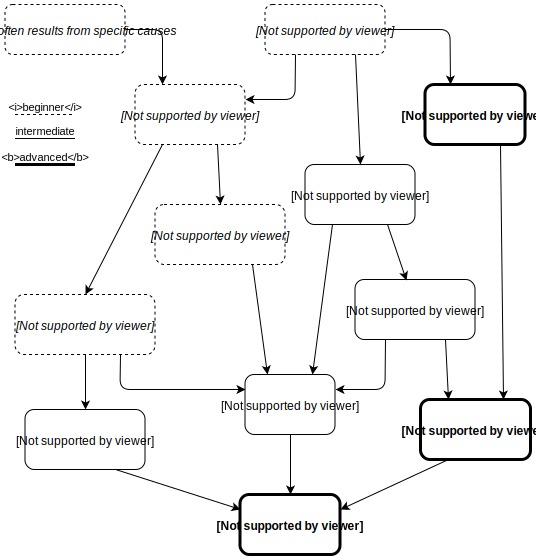
\includegraphics{../docs/fig/conditionals.pdf}
\caption{Learning Trajectory for Conditions (from \cite{Rich2017})}
\label{f:pck-trajectory}
\end{figure}

\section{How Much Are Novices Learning?}\label{s:pck-baseline}

Study after study has shown that teaching evaluations don't correlate
with actual learning outcomes \cite{Star2014,Uttl2017}, so to find out
how much novices are actually learning, we have to use other measures
or do direct studies.  Taking the former approach, roughly two-thirds
of post-secondary students pass their first computing course, with
some variations depending on class size and so on, but with no
significant differences over time or based on language
\cite{Benn2007a,Wats2014}.

Taking the latter approach, \cite{McCr2001} presented a multi-site
international study, which was later replicated by \cite{Utti2013}.
According to the first study, ``{\ldots}the disappointing results
suggest that many students do not know how to program at the
conclusion of their introductory courses.''  More specifically, ``For
a combined sample of 216 students from four universities, the average
score was 22.89 out of 110 points on the general evaluation criteria
developed for this study.''  However, this may say as much about
teachers' expectations as it does about student ability.

A growing number of studies have looked at how prior experience
affects these results.  For example, \cite{Wilc2018} compared the
performance and confidence of novices with and without prior
programming experience in CS1 and CS2.  They found that novices with
prior experience outscored novices without by 10\% in CS1, but those
differences disappeared by the end of CS2.  They also found that women
with prior exposure outperformed their male peers in all areas, but
were consistently less confident in their abilities; we will return to
this issue in \secref{s:motivation-inclusivity}.

\section{Do Languages Matter?}\label{s:pck-language}

The short answer is ``yes'': novices learn to program faster and also
learn more using blocks-based tools like Scratch
(\figref{f:pck-scratch}) that make syntax errors impossible
\cite{Wein2017b}.  And block interfaces encourage exploration in a way
that text does not; like all good tools, Scratch can be learned
accidentally \cite{Malo2010}.

\begin{figure}
\centering
\includegraphics{../docs/fig/scratch.jpg}
\caption{Scratch (from \url{https://opensource.com/article/18/4/designing-game-scratch-open-jam})}
\label{f:pck-scratch}
\end{figure}

\cite{Mlad2017} studied 207 novices learning about loops in Scratch,
Logo, and Python, and found that misconceptions about loops are
minimized when using a block-based language rather than a text-based
language.  What's more, as tasks become more complex (such as using
nested loops) the differences become larger.  Similarly,
\cite{Grov2017} studied 100 middle-school children, they found that
while it was easier for them to assemble programs with blocks than
with text.  However, some concepts are still intrinsically hard, such
as loops that modify variables and logical \texttt{or} (which is often
interpreted as ``one or the other'' rather than ``one or both'').

Scratch has probably been studied more than any other programming
tool, and we know a great deal about how it is used.  For example,
\cite{Aiva2016} analyzed over 250,000 Scratch projects and found among
other things that about 28\% of projects have some blocks that are
never called or triggered.  The authors hypothesize that users may be
using them as a scratchpad to keep bits of code they don't (yet) want
to throw away.

\cite{Wein2017a} studied people using a tool that allowed them to
switch between blocks and text for programming.  They found that
learners tend to migrate from blocks to text over time, but there are
interesting exceptions.  In two thirds of the cases where learners
shifted from text to blocks, their next action was to add a new type
of command; this may be because browsing available commands is easier
with blocks, or because blocks make syntax errors with unfamiliar new
commands impossible.

Learners also shifted from text to blocks when adding complex control
(e.g., an \texttt{if} with an \texttt{else}), either because syntax
errors are harder, or because the flow of control is immediately
visible.  The authors say, ``While it is often claimed that
blocks-based programming environments offer the advantage of reducing
syntax errors, our findings suggest that blocks also offer information
about what is possible in the space and provide a low-stakes means of
exploring unfamiliar code.''  New tools like
\href{https://www.greenfoot.org/frames/}{Stride} are trying to smooth
the transition between blocks and text even further; when combined
with programming notebooks like \href{http://jupyter.org/}{Jupyter}
and \href{http://stenci.la/}{Stencila}, they may eventually eliminate
the distinction altogether.

\subsection*{Object-Oriented Programming and Functional Programming}

Objects and classes are power tools for experienced programmers, and
many educators advocate an ``objects first'' approach to teaching
programming (though they sometimes disagree on exactly what that means
\cite{Benn2007b}).  \cite{Sorv2014} describes and motivates this
approach, and \cite{Koll2015} describes three generations of tools
designed to support novice programming in object-oriented
environments.

Introducing objects early has a few challenges.  For example,
\cite{Mill2016b} found that most novices using Python had difficulty
with \texttt{self} (which refers to ``this object''): they omitted it
in method definitions, failed to use it when referencing object
attributes, or both.  Object reference errors were also more common
than other errors; the authors speculate that this is partly due to
the difference in syntax between \texttt{obj.method(param)} and
\texttt{def method(self, param)}.  \cite{Rago2017} found something
similar in a study of 86 high school students.  They also found that
high school teachers often weren't clear on the concept either.

Yet another approach is exemplified by the
\href{http://www.bootstrapworld.org/}{Bootstrap project}, which is
based on the \glossref{g:functional-programming}{functional
  programming} paradigm.  This work draws on a rich tradition going
back to languages like Scheme and Lisp, and to classic textbooks like
\cite{Fell2001}, \cite{Frie1995}, and \cite{Abel1996}.  As functional
programming continues to gain ground among professional programmers,
this approach to teaching may continue to grow more popular.

\subsection*{Type Declarations}

Programmers argue a lot about whether variables' data types should
have to be declared or not.  One recent non-educational finding is
\cite{Gao2017}, which selected fixed bugs from public JavaScript
projects, checked out the code from version control just prior to the
fix, manually added type annotations to the buggy code, and then
tested whether strongly-typed variants of JavaScript reported an
error.  They found that about 15\% of bugs are caught, which is either
high or low depending on what answer you wanted in the first place.

However, programming and learning to program are different activities,
and results from the former don't necessarily apply to the latter.
\cite{Endr2014} found that requiring novices to declare variable types
does add some complexity to programs, but it pays off fairly quickly
by acting as documentation for a method's use---in particular, by
forestalling questions about what's available and how to use it.

\subsection*{Will Things Get Better?}

\cite{Stef2013} has shown that the creators of programming language
make those languages harder to learn by not doing basic usability
testing.  For example, ``{\ldots}the three most common words for
looping in computer science, \texttt{for}, \texttt{while}, and
\texttt{foreach}, were rated as the three most unintuitive choices by
non-programmers.''  More fundamentally, their work shows that C-style
syntax (as used in Java and Perl) is just as hard for novices to learn
as a randomly-designed syntax, but that the syntax of languages such
as Python and Ruby is significantly easier to learn, and the syntax of
their own language, Quorum, is easier still, because they are testing
each new feature before adding it to the language. (\cite{Stef2017} is
a useful brief summary of what we actually know about designing
programming languages and why we believe it's true.)

However, none of this matters unless designers are willing to take it
into account, and they are often reluctant to do so.  For example,
\cite{Pere2013} compared the actual operation of Git (a popular
version control system) with its users' conceptual model, highlighting
and explaining the many errors and confusion that result from the
differences.  \cite{Pere2016} then used that work to design a more
user-friendly alternative to Git.  The result?

\begin{quote}

  In sharing our research with colleagues{\ldots}we have discovered a
  significant polarization. Experts, who are deeply familiar with the
  product, have learned its many intricacies, developed complex,
  customized workflows, and regularly exploit its most elaborate
  features, are often defensive and resistant to the suggestion that
  the design has flaws. In contrast, less intensive users, who have
  given up on understanding the product, and rely on only a handful of
  memorized commands, are so frustrated by their experience that an
  analysis like ours seems to them belaboring the obvious.

\end{quote}

\section{Can We Give Better Feedback?}\label{s:pck-error}

Incomprehensible error messages are a major source of frustration for
novices (and sometimes for experienced programmers as well).  Several
researchers have explored whether better error messages would help
alleviate this.  For example, \cite{Beck2016} wrote some for the Java
compiler so that instead of:

\begin{verbatim}
C:\stj\Hello.java:2: error: cannot find symbol
        public static void main(string[ ] args){
^
1 error
Process terminated ... there were problems.
\end{verbatim}

\noindent
learners would see:

\begin{verbatim}
Looks like a problem on line number 2.
If "string" refers to a datatype, capitalize the 's'!
\end{verbatim}

\noindent
Novices given these messages made fewer repeated errors and fewer
errors overall.

\cite{Bari2017} went further and used eye tracking to show that
despite the grumblings of compiler writers, people really do read
error messages---in fact, they spend 13--25\% of their time on task
doing this.  Reading error messages turns out to be as difficult as
reading source code, and how difficult it is to read the error
messages strongly predicts task performance.  The inescapable
conclusion is that it really is important to get this right, and that
error messages should be usability tested the same way as any other
interface.

Since interpreting and responding to error messages is important,
instructors should give learners exercises that do just that.
\cite{Marc2011} has a rubric for responses to error messages that can
be useful in grading such exercises.

\section{Does Variable Naming Style Matter?}\label{s:pck-code}

\cite{Kern1999} says, ``Programmers are often encouraged to use long
variable names regardless of context. This is a mistake: clarity is
often achieved through brevity.''  Lots of programmers believe this,
but \cite{Hofm2017} found that using full words in variable names led
to an average of 19\% faster comprehension compared to letters and
abbreviations, with no significant difference in speed between single
letters and abbreviations, but didn't look at \emph{which} names were
abbreviated.

For that, we have to turn to \cite{Beni2017}, which found that using
single-letter variable names doesn't affect novice programmers'
ability to modify code.  This may be because novices' programs are
shorter than professionals', but it may also be because some
single-letter variable names have implicit types and meanings: most
programmers assume \texttt{i}, \texttt{j}, and \texttt{n} are
integers, and \texttt{s} is a string, while \texttt{x}, \texttt{y},
and \texttt{z} are either floating-point numbers or integers more or
less equally.

How important is this?  \cite{Bink2012} reported a series of studies
that found that reading and understanding code is fundamentally
different from reading prose: ``{\ldots}the more formal structure and
syntax of source code allows programmers to assimilate and comprehend
parts of the code quite rapidly independent of style.  In
particular{\ldots}beacons and program plans play a large role in
comprehension.''  It also found that experienced developers are
relatively unaffected by identifier style (although again, they didn't
explore \emph{which} variables), and that beginners found CamelCase
easier to read than pothole\_case.  This is surprising because word
spacing improves readability in conventional tasks.  Digging deeper,
``{\ldots}camel casing produces more accurate results.  However, this
correctness comes at a cost as the camel-case style significantly
increases the time needed to correctly detect the correct
identifier.''

\section{Does Visualization Help?}\label{s:pck-visualization}

The idea of visualizing programs is perennially popular, and tools
like \cite{Guo2013} (a web-based tool for visualizing the execution of
Python programs) and \href{http://latentflip.com/loupe/}{Loupe} (which
shows how JavaScript's event loop works) are both popular teaching
aids.  However, we have known for over 20 years that people learn more
from constructing visualizations than they do from viewing
visualizations constructed by others \cite{Stas1998,Ceti2016}, so does
visualization actually helping learning?

To answer this, \cite{Cunn2017} replicated an earlier study of the
kinds of sketching students do when tracing code execution, and
correlations between different kinds and effectiveness.  Different
rates of sketching for different problems indicated that students use
it to externalize cognition; not sketching at all correlates with
lower success, while tracing changes to variables' values by writing
new values near their names as they change was the most effective
strategy.

One possible confounding effect they checked was time: since sketchers
take significantly more time to solve problems, do they do better just
because they think for longer?  The answer is no: there was no
correlation between the time taken and the score achieved.  To the
best of my knowledge, nobody has yet built a debugger that shows
successive values for variables laid out in rows, but this research
suggests that something like that could help.

\begin{callout}{Flowcharts}

  One often-overlooked finding about visualization is that students
  understand flowcharts better than pseudocode \emph{if both are
    equally well structured} \cite{Scan1989}.  Earlier work showing
  that pseudocode outperformed flowcharts used structured pseudocode
  and tangled flowcharts; when the playing field was levelled, novices
  did better with the graphical representation.

\end{callout}

\section{What Else Can We Do to Help?}\label{s:pck-help}

\cite{Viha2014} examined the average improvement in pass rates of
various kinds of intervention in programming classes.  As they
themselves point out, there are many reasons to take their findings
with a grain of salt: the pre-change teaching practices are rarely
stated clearly, the quality of change is not judged, and only 8.3\% of
studies reported negative findings, so either there is positive
reporting bias or the way we're teaching right now is almost the worst
way possible and anything would be an improvement.  It's also worth
remembering that like almost all of the studies discussed in this
chapter, they were only looking at university classes: their findings
may not generalize to other groups.

With all those caveats in mind, they found ten things instructors can
do to improve outcomes.  \figref{f:pck-interventions} shows the
average improvement reported for each type:

\begin{description}

\item[Collaboration:] % (20/34\%)
  Activities that encourage student collaboration either in classrooms
  or labs.

\item[Content Change:] % (36/34\%)
  Parts of the teaching material were changed or updated.

\item[Contextualization:] % (17/40\%)
  Course content and activities were aligned towards a specific
  context such as games or media.

\item[CS0:] % (7/43\%)
  Creation of a preliminary course to be taken before the introductory
  programming course; could be organized only for some (e.g., at-risk)
  students.

\item[Game Theme:] % (9/18\%)
  A game-themed component was introduced to the course.

\item[Grading Scheme:] % (11/29\%)
  A change in the grading scheme; the most common change was to
  increase the amount of points rewarded from programming activities,
  while reducing the weight of the course exam.

\item[Group Work:] % (7/45\%)
  Activities with increased group work commitment such as team-based
  learning and cooperative learning.

\item[Media Computation:] % (10/48\%)
  Activities explicitly declaring the use of media computation
  (\chapref{s:motivation}).

\item[Peer Support:] % (23/34\%)
  Support by peers in form of pairs, groups, hired peer mentors or
  tutors.

\item[Other Support:] % (9/33\%)
  An umbrella term for all support activities, e.g. increased teacher
  hours, additional support channels, etc.

\end{description}

\begin{figure}
\centering
\includegraphics{../docs/fig/interventions.png}
\caption{Effectiveness of Interventions}
\label{f:pck-interventions}
\end{figure}

This list highlights the importance of cooperative learning.
\cite{Beck2013} looked at this specifically over three academic years
in courses taught by two different instructors, and found significant
benefits overall and for many subgroups: they not only had higher
grades, they left fewer questions blank on the final exam, which
indicates greater self-efficacy and willingness to try to debug
things.

As noted earlier, writing code isn't the only way to teach people how
to program.  \cite{Shel2017} reports that having novices work on
computational creativity exercises improves grades at several levels.
A typical exercise is to identify an everyday object (such as nail
clipper, a paper clip, Scotch tape) and describe the object in terms
of its inputs, outputs and functions.  This kind of teaching is
sometimes called ``unplugged'', and the
\href{https://csunplugged.org/en/}{CS Unplugged} site has a collection
of lessons and exercises for doing this.

\section{Exercises}\label{s:pck-exercises}

\exercise{Checking for Common Errors}{individual}{20}

This list of common errors is taken from \cite{Sirk2012}.  Pick three,
and write an exercise for each to check that learners \emph{aren't}
making that mistake.

\begin{description}

  \item[Inverted assignment:] The student assigns the value of the
    left-hand variable to the right-hand side variable, rather than
    the other way around.

  \item[Wrong branch:] Even though the conditional evaluates to
    \texttt{False}, the student jumps to the \texttt{then} clause.

  \item[Wrong \texttt{False}:] As soon as the conditional evaluates to
    \texttt{False} , the student returns \texttt{False} from the
    function.
  
  \item[Executing function instead of defining it:] The student
    believes that a function is executed as it is defined.

  \item[Unevaluated parameters:] The student believes the function
    starts running before the parameters have been evaluated.

  \item[Parameter evaluated in the wrong frame:] The student creates
    parameter variables in the caller's frame, not in the callee's.

  \item[Failing to store return value:] The student does not assign
    the return value in the caller.

  \item[Assignment copies object:] The student creates a new object
    rather than copying a reference.

  \item[Method call without subject:] The student tries to call a
    method from a class without first creating an instance of the
    class.

\end{description}

\exercise{Mangled Code}{pairs}{15}

\cite{Chen2017} describes exercises in which students reconstruct code
that has been mangled by removing comments, deleting or replacing
lines of code, moving lines, inserting extra unneeded lines, and so
on.  Student performance on these correlates strongly with performance
on assessments in which students write code (i.e., whatever
traditional assignments are measuring, these are measuring as well),
but these questions require less (in-person) work to mark.  Take the
solution to a programming exercise you've created in the past, mangle
it in two different ways, and swap with a partner.

\exercise{The Rainfall Problem}{pairs}{10}

Solve the Rainfall Problem in the programming language of your choice
in two different ways. Compare your solutions with those of your
partner.

\exercise{Roles of Variables}{pairs}{15}

Take a short program you have written (5--15 lines) and classify each
of its variables using the categories defined in
\secref{s:pck-programming}.  Compare your classifications with those
of a partner: where did you agree? When you disagreed, did you
understand each other's view?

\exercise{Choose Your Own Adventures}{individual}{10}

Which of the three approaches described in \cite{Sorv2014}
(\secref{s:pck-now}) do you use when teaching? Or is your approach
best described in some other way?

\exercise{What Are You Teaching?}{individual}{10}

Compare the topics you teach to the list developed in \cite{Luxt2017}
(\secref{s:pck-now}).  Which topics do you cover?  What extra topics
do you cover that aren't in their list?

\exercise{Beneficial Activities}{individual}{10}

Look at the list of interventions developed by \cite{Viha2014}
(\secref{s:pck-help}).  Which of these things do you already do in
your classes?  Which ones could you easily add?  Which ones are
irrelevant?

\exercise{Visualizations}{individual}{10}

What visualization do you most like to use when teaching?  Is it a
static image or an animation?  Do you show it to your learners, do
they discover it on their own, or something in between?

\exercise{Misconceptions and Challenges}{small groups}{15}

The \href{http://www.pd4cs.org/}{Professional Development for CS
  Principles Teaching} site includes
\href{http://www.pd4cs.org/mc-index/}{a detailed list of student
  misconceptions and exercises}.  Working in small groups, choose one
section (such as data structures or functions) and go through their
list.  Which of these misconceptions do you remember having when you
were a learner?  Which do you still have?  Which have you seen in your
learners?

\chapter{Enseñar como un arte performativo}\label{s:performance}

En \emph{Darwin entre las máquinas},
George Dyson\index{Dyson, George} escribió,
``En el juego de la vida y la evolución hay 3 jugadores en la mesa:
los humanos, la naturaleza y las máquinas.
Estoy firmemente del lado de la naturaleza.
Pero la naturaleza, sospecho, está del lado de las máquinas{\ldots}''
De manera similar, ahora hay 3 jugadores en el juego de la educación:
los libros de texto y otros materiales de lectura,
las clases en vivo,
y las clases en línea automatizadas.
Podrías darle a tus estudiantes clases escritas y alguna combinación
de videos grabados y ejercicios para que realicen a su propio ritmo,
pero si vas a enseñar en persona tienes
que ofrecer algo diferente (y con suerte mejor que) cualquiera de los anteriores.
Por lo tanto, este capítulo se enfoca en cómo enseñar a programar programando.

\seclbl{Programar en vivo}{s:performance-live}

\begin{quote}

  La enseñanza es teatro, no cine. \\
  --- Neal Davis\index{Davis, Neal}

\end{quote}

La manera más efectiva de enseñar a programar es \gref{g:live-coding}{programando en vivo}~\cite{Rubi2013,Haar2017,Raj2018}.
En vez de presentar material previamente escrito,
quien enseña escribe el código en frente de la clase
mientras que los/las estudiantes lo siguen a la par,
escribiendo y ejecutándo el código a medida que avanzan.
Programar en vivo funciona mejor que las presentaciones por varias razones:

\begin{itemize}

\item
  Permite la \gref{g:active-teaching}{enseñanza activa}
  al permitir a quienes están enseñando responder a los intereses y preguntas de los/las estudiantes en el momento.
  Una presentación de diapositivas es como una vía de ferrocarril:
  podrá ser un viaje suave,
  pero tienes que decidir hacia donde vas con anticipación.
  Programar en vivo es cómo manejar un vehículo todo terreno:
  podrá ser más accidentado,
  pero es mucho más fácil cambiar de dirección e ir hacia donde la gente quiere.

\item
  Mirar como se va escribiendo un programa es más motivador
  que mirar a alquien pasar diapositivas.

\item
  Facilita la transferencia de conocimiento de manera involuntaria:\index{unintended knowledge transfer}
  las personas aprenden más de lo que enseñamos conscientemente
  al observar \emph{cómo} hacemos las cosas.

\item
  Disminuye la velocidad de la persona que está enseñando:
  si tiene que escribir el programa medida que avanza,
  entonces solo puede ir el doble de rápido que sus estudiantes
  en vez de 10 veces más rápido como lo harían usando diapositivas.

\item
  Ayuda a reducir la carga en la memoria de corto plazo
  porque hace que quien esté enseñando se más consciente de cuanto 
  le está mostrando a sus estudiantes.

\item
  Los/Las estudiantes pueden ver cómo diagnosticar y corregir errores.
  Van a dedicar mucho tiempo a esto;
  a menos que puedan tipear de manera perfecta,
  programar en vivo asegura que puedan ver como hacer esto.

\item
  Ver a quienes enseñan cometer errorer muestra a sus estudiantes que está bien que cometan errores.
  Si el/la docente no se avergüenza al cometer errores y habla sobre ellos,
  sus estudiantes también se sentirán más cómodos/as hacíendolo.

\end{itemize}

Otro beneficio de la programación en vivo es que demuestra el orden en que se deben escribir los programas.
Cuando observaron cómo las personas resuelven problemas de Parson,\index{Parsons Problem}
\cite{Ihan2011} encontraron que las personas con experiencia programando usualmente ubican la identificación del método al principio,
luego agregan la mayor parte del control de flujo (es decir, bucles y condiciones),
y solo luego de eso, agregan detalles como la inicialización de variables y el manejo de casos especiales.
Es método ``fuera de orden'' es ajeno para las personas novatas,
que leen y escriben código en el orden en que se presenta en la página;
ver el código les ayuda a descomponer los problemas en submetas que pueden abordar una a la vez.
La programación en vivo además les da quienes están enseñando la chance de enfatizar la importancia de los pequeños pasos con comentarios frecuentes~\cite{Blik2014}
y la importancia de definir un plan en vez de hacer 
cambios más o menos aleatorios y esperar que las cosas mejoren~\cite{Spoh1985}.

Sentise cómodo/a al hablar mientras se escribe código en 
frente de una audiencia, requiere práctica,
pero la mayoría de las personas indican que rápidamente se vuelve igual que difícil que hablar alrededor de una presentación de diapositivas.
Las secciones que siguen ofrecen consejos sobre cómo mejorar la manera de programar en vivo.

\subsection*{Aprovecha tus errores}

\begin{quote}

  Los errores de tipeo son la pedagogía. \\
  --- Emily Jane McTavish\index{McTavish, Emily Jane}

\end{quote}

La regla más importante de la programación en vivo es aprovechar tus errores.\index{mistakes (importance of embracing)}
No importa que tan bien te prepares, 
cometerás algunos errores;
cuando lo hagas,
piensa sobre ellos con tu audiencia.
Si bien obtener los datos es difícil,
programadores/as profesionales dedican del 25\% al 60\% de su tiempo identificando y resolviendo errores;
las personas novatas dedican le dedicanmucho más (\secref{s:pck-debug}),
pero la mayoría de los libros de texto y tutoriales dedican poco tiempo a diagnosticar y corregir problemas.
Si hablas en voz alta mientras intentas identificar que escribiste mal
o dónde tomaste el camino equivocado,
y explicas cómo lo corriges,
les darás a tus estudiantes un conjunto de herramientras que pueden usar cuando comentan sus propios errores.

\begin{aside}{Tropiezos deliberados}
  Una vez que hayas enseñado una lección varias veces,
  es poco probable que cometas nada más que errores básicos de tipeo
  (que de todas maneras pueden ser informativos).
  Puede intentar recordar errores pasados y cometerlos deliberadamente,
  pero usualmente eso se siente forzado.
  Un enfoque alternativo es \gref{g:twitch-coding}{sacudir la programación}:
  pide a tus estudiantes, uno a uno que te indiquen que escribir a continnuación.
  Esto practicamente garantiza que te encuentres en algún tipo de problemas.
\end{aside}

\subsection*{Pregunta por predicciones}

Una manera de mantener a tus estudiantes motivados/as mientras estas programando en vivo
es pedirles que hagan predicciones sobre que hará el código que ven en la pantalla.
Luego, puedes escribir las primeras sugerencias que hagan,
hacer que toda la clase vote sobre cúal piensan que es la opción más probable,
y finalmente ejecutar el código.
Esta es una forma simple de instrucción entre pares,\index{peer instruction}
que discutiremos en la sección \secref{s:classroom-peer};
además de mantener su atención en la actividad,
les permite practicar cómo razona sobre el comportamiento del código.

\subsection*{Tomalo con calma}

Cada vez que escribas un comando,
agregues una lidea de código a un programa,
o selecciones un elemento de un menú,
di que estas haciendo en voz alta,
luego señala lo que haz hecho y su resultado en la pantalla
y repasalo una segunda vez.
Esto ayuda a tus estudiantes a ponerse al día
y a revisar que lo que acaban de hacer es correcto.
Esto es particularmente importante cuando algunos de tus estudiantes tienen dificultades para ver o escuchar o no dominan el idioma en el que estás enseñando.

Hagas lo que hagas,
\emph{no} copies y pegues códgio:
hacer eso practicamente garantiza que iras mucho más rápido que tus estudiantes.
Y si usas la tecla tab para autocompletar lo que estás escribiendo,
decilo en vos alta para que tus estudiantes entiendan lo que estás haciendo:
``Usemos turtle dot `r' `i' y tab para completar con `right'.''

Si la salida de tu comando o código hace que lo que acabas de escribir desaparezca de la vista,
volvé arriba para que tus estudiantes puedan verlo de nuevo.
Si eso no es posible,
ejecuta el mismo comando una segunda vez
o copia y pega el último comando o comandos en las notas compartidas del taller.

\subsection*{Ser visto/a y escuchado/a}

Cuando te sientas,
es más probable que mires tu pantalla en vez de mirar a tu audiencia
y puedes quedar fuera de la vista de tus estudiantes en las últimas filas del aula.
Si eres físicamente capaz de pararte durante un par de horas,
debes hacerlo mientras enseñas.
Planifíscalo y asegúrate de tener una mesa elevada, 
un escritorio de pie,
o un atril
para tu computadora portátil
para que no tengas que inclinarte al escribir.

Independientemente de si estás de pie o sentado/a,
asegurate de moverte lo más que puedas:
acercate a la pantalla para señalar algo,
dibuja algo en la pizarra,
o simplemente alejate de la computadora por un momento y hablale directamente a tu audiencia.
Hacer esto aleja la atención de tus estudiantes de sus pantallas
y les proporciona un mmomento natural para hacer preguntas.

Si vas a enseñar por más de un par de horas,
vale la pena usar un micrófono incluso si la habitación es pequeña.
Tu garganta se cansa tanto como cualquier otra parte de tu cuerpo;
usar un micrófono no es diferente de usar zapatos cómodos 
(algo que también deberías usar).
También puede marcar una gran diferencia para las personas que tienen discapacidad auditiva.

\subsection*{Copia la pantalla de tu estudiante}

Es posible que hayas personalizado tu entorno de trabajo con una terminal de Unix shell elegante,
un esquema de colores personalizado,
o una gran cantidad de atajos de teclado.
Tu estudiantes no tendrán nada de eso,
así que intenta crear un entorno de trabajo que refleje lo que \emph{sí} tienen.
Algunos/as docentes crean un usuario distinto con configuración básica en sus computadoras
o una cuenta específica para enseñar 
si están usando algún servicio online como Scratch o GitHub.
Hacer esto también puede ayudar a evitar que los paquetes que instalaste ayer para trabajar 
rompan la lección que se supone que enseñes hoy.

\subsection*{Usa la pantalla de menera sabia}

Por lo general, necesitaras agrandar el tamañana de la letra considerablemente
para que las personas en el fondo de la sala puedan leer. 
Esto significa que podrás colocar muchas menos cosas en la pantalla de las que estás acostumbrado/a.
En muchos casos, se reducirá a 60--70 columnas y 20--30 filas,
por lo que estarás usando una super computadora del siglo 21
como si fuera una sencilla terminal de principios de la década de 1980.

Para organizar esto,
maximiza la ventana que estás usando para enseñar
y luego preguntale a todos si pueden leer lo que están en la pantalla o no.
Usa una fuente de color negro sobre un fondo ligeramente coloreado en vez de una fuente de color claro sobre un fondo oscuro---el tono claro deslubrará 
menos que el blanco puro.

Presta atención a la iluminación de la sala:
no debe estar completamente a oscuras, y no debe haber luces directamente 
o por encima de la pantalla de protección.
Dedica algunos minitos para que tus estudiantes puedan reacomodar sus mesas
para ver con claridad.

Cuando la parte inferior de la proyección de la pantalla está a la misma altura que las cabezas de tus estudiantes,
las personas en el fondo no podrán ver lo que ocurre en esa sección de la pantalla.
Puede elevar la parte inferior de la ventana para compesar esto,
pero eso generará que tengas aún menos espacio para escribir.

Si puedes acceder a un segundo proyector y pantalla,
usalos:
el espacio adicional te permitirá mostrar el código de un lado
y su resultado o comportamiento del otro lado.
Si la segunda pantalla requiere su propia computadora,
pidele a un/a ayudante que la controle
en lugar de ir y venir entre los dos teclados.

Finalmente,
si estás enseñando algo como la terminal de Unix shell en una consola,
es importante decirle a las personas usas un editor de texto en la consola
y cuando regresas a la consola propiamente dicha.
La mayoría de las personas novatas no han visto nunca una ventana asumir multiples personalidades de esta manera,
y pueden confundirse rápidamente
cuando estás interactuando en la terminal,
cuando estás escribiendo en un editor de texto,
y cuando estás trabajando de manera interactiva con Python u otro lenguaje.
Puedes evitar este problema usando ventanas separadas para usar el editor de texto;
si haces esto,
siempre avísales a tus estudiantes cuando estás cambiando de una ventana a la otra.

\begin{aside}{Las herramientas de accesibilidad ayudan a todas las personas}
  Las herramientas como \hreffoot{https://boinx.com/mousepose/overview/}{Mouseposé} (para Mac)
  y \hreffoot{http://www.pointerfocus.com/}{PointerFocus} (para Windows)
  resaltan la posición del cursor del mouse en la pantalla,
  y las herramientras de grabación de pantalla como \hreffoot{https://www.techsmith.com/video-editor.html}{Camtasia}
  y aplicaciones independientes como \hreffoot{https://github.com/keycastr/keycastr}{KeyCastr}
  muestran teclas invisibles como tab y Control-J a medida que las usas.
  Esto puede ser un poco molesto al comienzo,
  pero ayuda a tus estudiantes a descubrir lo que estás haciendo.
\end{aside}

\subsection*{Dos dispositivos}

Algunas personas usan dos dispositivos cuando enseñan:
una computadora portatil conectada al proyector que los/as estudiantes vean
y una tablet para que puedan ver sus propias notas y las notas que los/as estudiantes están tomando (\secref{s:classroom-notetaking}).
Esto es más confiable que pasar de un escritorio virtual al otro, 
aunque imprimir la lección sigue siendo la técnología de respaldo más confiable.

\subsection*{Dibuja temprano, dibuja seguido}

Los diagramas son siempre una buena idea.
A veces tengo una presentación de diapostivas llena de diagramas preparada de antemano,
pero construir los diagramas paso a paso ayuda a retenerlos más (\secref{s:architecture-brain})
y te permite improvisar.

\subsection*{Evita las distracciones}

Desactiva las notificaciones que usas en tu computadora,
espcialmente las de redes sociales.
Ver mensajes parpadeando en la pantalla te distrae a vos y a tus estudiantes,
y puede ser incómodo si aparece un mensaje que no te gustaría que otras personas vean.
De nuevo,
es posible que quieras crear una segunda cuenta en tu computadora que no tenga correo electrónico u otras herramientas configuradas.

\subsection*{Improvisa---luego de haber aprendido el material}

No te alejes de la lección que planificaste o pediste prestada la primera vez que la enseñes.
Puede ser tentandor desviarse del material
porque te gustaría mostrar un lindo truco o demostrar otra manera de hacer algo,
pero existe la posibilidad de que te encuentres con algo inesperado 
que te lleve más tiempo del que tenés.

Sin embargo, una vez que el material te resulte más familiar,
puedes y debes comenzar a improvisar en base a los antecedentes de tus estudiantes,
sus preguntas durante la clase,
y lo que personalmente te parezca más interesante.
Esto es como tocar una nueva canción:
sigues la partitura las primeras veces,
pero después de que te sientes comodo/a con los cambios de melodía y acordes,
puedes comenzar a ponerle tu propio sello.

Cuando quieras usar algo nuevo,
revísalo de antemano
\emph{usando la misma computadora que usarás cuando des la clase}:
instalar cientos de megabytes de programas a través del WiFi de la escuela secundaria
en frente de joneves de 16 años aburridos no es algo por lo que alguna vez quieras pasar.

\begin{aside}{Enseñanza directa}
  La \gref{g:direct-instruction}{Enseñanza directa} (ED) es un método de enseñanza
  centrando en el diseño meticuloso de la currícula dictado usando un guío predefinido.
  Es más como un actor recitando lineas que como el enfoque de inprovisación que recomendamos.
  \cite{Stoc2018} encontró que la ED tiene un efecto estadísticamente significativo positivo 
  a pesar de que a veces pueda ser muy repetitivo.
  Yo prefiero improvisar porque la ED requiere más preparación inicial que lo que la mayoría 
  de los grupos de estudiantes free-range pueden permitirse.
\end{aside}

\subsection*{Mira a la pantalla---de vez en cuando}

Está bien enfrentar la pantalla donde estás proyectando ocacionalmente
cuando estás mostrando una sección de código o dibujando un esquema:
\emph{no} mirar a la sala llena de personas que te están mirando a vos
puede ayudarte a reducir tu nivel de ansiedad y darte un momento para pensar qué decir a continuación.

Sin embargo, no deberías hacerto por más de unos segundos.
Una buena regla general es tratar a la pantalla como a uno/a de tus estudiantes:
si mirar a una persona durante el tiempo que miras a la pantalla te resulta incómodo, es hora de darte la vuelta y mirar a la clase nuevamente.

\subsection*{Incovenientes}

Porgramar en vivo tiene algunos inconvenientes,
pero pueden evitarse o solucionarse con un poco de práctica.
Si descrubres que están cometiendo demasiados errores de tipeo,
reserva 5 minutos por día para practicar escribir con el teclado:
también te ayudará en tu trabajo diario.
Si crees que dependes demasiado de las notas de la clase,
divídelas en partes más pequeñas 
para que solo tengas que pensar en un pequeño paso a la vez.

Y si sientes que estás pasando demasiado tiempo escribiendo código para importar librerías, encabezados de clases y código repetitivo, 
genera un esqueleto de código para que vos y tus estudiantes usen como punto de partida (\secref{s:classroom-blank}).
Hacer esto también reducirá su carga cognitiva,
dado que centrarán su atención donde vos quieres.

\seclbl{Estudiar la lección}{s:performance-jugyokenkyu}

Desde políticos hasta investigador/as y docentes,
quines reforman la educación han diseñado sistemas 
para encontrar y apoyar a personas que pueden enseñar bien
y eliminar a las personas no lo hacen.
Pero la suposición de que algunas personas nacen como docentes es errónea:
en cambio,
como cualquier otra representación artística,
las claves para enseñar mejor son práctica y colaboración.
Cómo explica~\cite{Gree2014},
En japonés este enfoque se llama \gref{g:jugyokenkyu}{jugyokenkyu},
que signofica ``estudiar la lección'':

\begin{quote}

  Para graduarse,
  los especialistas en educación [japoneses] no solo tenían que ver como trabaja el docente que le asignan,
  tenían que reemplazarlo efectivamente,
  participando en su aula primero como observadores/as y luego,
  a la tercera semana,
  como una aproximación{\ldots}titubeante del propio maestro.
  Funcionó como una especie de relevo de docentes.
  Cada estudiante eligió una asignatura,
  preparando clases para 5 días{\ldots} [y luego] cada uno enseñó un día.
  Para pasar la batuta,
  tenía que enseñar una clase de un día en cada asignatura:
  la que tenían planeada y las 4 que no{\ldots}
  y tenían que hacerlo delante de su maestro.
  Después, todos---el docente, los estudiantes para ser docentes,
  y a veces, uncluso un observador externo---se sentaban alrededor de una mesa
  para hablar de lo que observaron.

\end{quote}

Poner el trabajo bajo un microscopio para mejorarlo es común
en áreas tan diversas como la \hreffoot{https://en.wikipedia.org/wiki/W.\_Edwards\_Deming}{fabricación} y la múscia.
Un/a músico/o profesional,
por ejemplo,
analizará media docena de grabaciones de ``Body and Soul'' o ``Smells Like Teen Spirit'' antes de interpretarlas.
También recibirán comentarios de colegas musicos durante la práctica y después de las actuaciones.

Pero la retroalimentación continua no es parte de la cultura de la enseñanzan en la mayoría de los paises de habla inglesa.
Allí,
lo que sucede en el aula se queda en el aula:
quienes enseñan no miran las clases de sus colegas de manera regular,
por lo que no pueden tomar prestadas las buenas ideas de las demás personas.
Los/as docentes podrán acceder a los planes de clases y tareas de otros colegas,
la junta escolar o una editorial de libros de texto,
o revisar MOOCs en Internet,
pero cada persona tiene que descubrir
como dar las clases específicas en aulas específicas para estudiantes específicos/as.
Esto es particularmente cierto para personas voluntarias y docentes free-range
que participan en talleres y actividades fuera de la escuela.

Writing up new techniques
and giving \grefdex{g:demonstration-lesson}{demonstration lessons}{demonstration lesson}
(in which one person teaches actual learners while other teachers observe)
are not solutions.
For example,
\cite{Finc2007,Finc2012} found that of the 99 change stories analyzed,
teachers only searched actively for new practices or materials in three cases,
and only consulted published material in eight.
Most changes occurred locally,
without input from outside sources,
or involved only personal interaction with other educators.
\cite{Bark2015} found something similar:

\begin{quote}

  Adoption is not a ``rational action''{\ldots}but
  an iterative series of decisions made in a social context,
  relying on normative traditions, social cueing,
  and emotional or intuitive processes{\ldots}
  Faculty are not likely to use educational research findings
  as the basis for adoption decisions{\ldots}
  Positive student feedback is taken as strong evidence by faculty
  that they should continue a practice.

\end{quote}

\emph{Jugyokenkyu} works because it maximizes the opportunity for unplanned knowledge transfer between teachers:
someone sets out to demonstrate X,
but while watching them,
their audience actually learns Y as well (or instead).
For example,
a teacher might intend to show learners how to search for email addresses in a text file,
but what their audience might take away is some new keyboard shortcuts.

\seclbl{Giving and Getting Feedback on Teaching}{s:performance-feedback}

Observing someone helps you,
and giving them feedback helps them,
but it can be hard to receive feedback,
especially when it's negative (\figref{f:performance-feedback-feelings}).

\figimg{figures/deathbulge-jerk.jpg}{Feedback feelings (copyright © Deathbulge 2013)}{f:performance-feedback-feelings}

Feedback is easier to give and receive when both parties share expectations
about what is and isn't in scope
and about how comments ought to be phrased.
If you are the person asking for feedback:
\index{feedback!getting}

\begin{description}

\item[Initiate feedback.]
  It's better to ask for feedback than to receive it unwillingly.

\item[Choose your own questions,]
  i.e.\ ask for specific feedback.
  It's a lot harder for someone to answer,
  ``What do you think?''
  than to answer either,
  ``Was I speaking too quickly?''
  or ,
  ``What is one thing from this lesson I should keep doing?''
  Directing feedback like this is also more helpful to you.
  It's always better to try to fix one thing at once
  than to change everything and hope it's for the better.
  Directing feedback at something you have chosen to work on helps you stay focused,
  which in turn increases the odds that you'll see progress.

\item[Use a feedback translator.]
  Have someone else read over all the feedback and give you a summary.
  It can be easier to hear,
  ``Several people think you could speed up a little,''
  than to read several notes all saying, ``This is too slow''
  or, ``This is boring.''

\item[Be kind to yourself.]
  Many of us are very critical of ourselves,
  so it's always helpful to jot down what we thought of ourselves
  \emph{before} getting feedback from others.
  That allows us to compare what we think of our performance
  with what others think,
  which in turn allows us to scale the former more accurately.
  For example,
  it's very common for people to think that they're saying ``um'' and ``err'' too often
  when their audience doesn't notice it.
  Getting that feedback once allows teachers to adjust their assessment of themselves
  the next time they feel that way.

\end{description}

\noindent
You can give feedback to others more effectively as well:
\index{feedback!giving}

\begin{description}

\item[Interact.]
  Staring at someone is a good way to make them feel uncomfortable,
  so if you want to give feedback on how someone normally teaches,
  you need to set them at ease.
  Interacting with them the way that a real learner would is a good way to do this,
  so ask questions or (pretend to) type along with their example.
  If you are part of a group,
  have one or two people play the role of learner
  while the others take notes.

\item[Balance positive and negative feedback.]
  The ``compliment sandwich'' made up of one positive comment,
  one negative,
  and a second positive
  becomes tiresome pretty quickly,
  but it's important to tell people what they should keep doing
  as well as what they should change\footnote{
    For a while,
    I was so worried about playing in tune that I completely lost my sense of timing.
  }.

\item[Take notes.]
  You won't remember everything you noticed
  if the presentation lasts longer than a few seconds,
  and you definitely won't recall how often you noticed them.
  Make a note the first time something happens
  and then add a tick mark when it happens again
  so that you can sort your feedback by frequency.

\end{description}

Taking notes is more efficient when you have some kind of rubric
so that you're not scrambling to write your observations
while the person you're observing is still talking.
The simplest rubric for free-form comments from a group
is a 2x2 grid whose vertical axis is labeled ``what went well'' and ``what can be improved'',
and whose horizontal axis is labeled ``content'' (what was said)
and ``presentation'' (how it was said).
Observers write their comments on sticky notes as they watch the demonstration,
then post those in the quadrants of a grid drawn on a whiteboard
(\figref{f:performance-rubric}).

\figpdf{figures/2x2-rubric.pdf}{Teaching rubric}{f:performance-rubric}

\begin{aside}{Rubrics and Question Budgets}
  \secref{s:checklists-teacheval} contains a sample rubric
  for assessing 5--10 minutes of programming instruction.
  It presents items in more or less the order that they're likely to come up,
  e.g.\ questions about the introduction come before questions about the conclusion.

  Rubrics like this one
  tend to grow over time as people think of things they'd like to add.
  A good way to keep them manageable is to insist that
  the total length stays constant:
  if someone wants to add a question,
  they have to identify one that's less important and can be removed.
\end{aside}

If you are interested in giving and getting feedback,
\cite{Gorm2014} has good advice
that you can use to make peer-to-peer feedback a routine part of your teaching,
while~\cite{Gawa2011} looks at the value of having a coach.

\begin{aside}{Studio Classes}
  Architecture schools often include studio classes\index{studio class}
  in which students solve small design problems
  and get feedback from their peers right then and there.
  These classes are most effective when the teacher critiques the peer critiques
  so that participants learn not only how to make buildings
  but how to give and get feedback~\cite{Scho1984}.
  Master classes in music serve a similar purpose,
  and I have found that giving feedback on feedback
  helps people improve their teaching as well.
\end{aside}

\seclbl{How to Practice Performance}{s:performance-practice}

The best way to improve your in-person lesson delivery
is to watch yourself do it:

\begin{itemize}

\item
  Work in groups of three.

\item
  Each person rotates through the roles of teacher, audience, and videographer.
  The teacher has 2 minutes to explain something.
  The person pretending to be the audience is there to be attentive,
  while the videographer records the session using a cellphone or other handheld device.

\item
  After everyone has finished teaching,
  the whole group watches the videos together.
  Everyone gives feedback on all three videos,
  i.e.\ people give feedback on themselves as well as on others.

\item
  After the videos have been discussed,
  they are deleted.
  (Many people are justifiably uncomfortable about images of themselves appearing online.)

\item
  Finally,
  the whole class reconvenes
  and adds all the feedback to a shared 2x2 grid of the kind described above
  \emph{without} saying who each item of feedback is about.

\end{itemize}

In order for this exercise to work well:

\begin{itemize}

\item
  Record all three videos and then watch all three.
  If the cycle is teach-review-teach-review,
  the last person to teach invariably runs short of time
  (sometimes on purpose).
  Doing all the reviewing after all the teaching
  also helps put a bit of distance between the two,
  which makes the exercise slightly less excruciating.

\item
  Let people know at the start of the class that they will be asked to teach something
  so that they have time to choose a topic.
  Telling them this too far in advance can be counter-productive,
  since some people will fret over how much they should prepare.

\item
  Groups must be physically separated to reduce audio cross-talk between their recordings.
  In practice,
  this means 2--3 groups in a normal-sized classroom,
  with the rest using nearby breakout spaces, coffee lounges, offices,
  or (on one occasion) a janitor's storage closet.

\item
  People must give feedback on themselves as well as on each other
  so that they can calibrate their impressions of their own teaching
  against those of other people.
  Most people are harder on themselves than they ought to be,
  and it's important for them to realize this.

\end{itemize}

The announcement of this exercise is often greeted with groans and apprehension,
since few people enjoy seeing or hearing themselves.
However,
those same people consistently rate it as one of the most valuable parts of teaching workshops.
It's also good preparation for co-teaching (\secref{s:classroom-together}):\index{co-teaching}
teachers find it a lot easier to give each other informal feedback
if they have had some practice doing so
and have a shared rubric to set expectations.

And speaking of rubrics:
once the class has put all of their feedback on a shared grid,
pick a handful of positive and negative comments,
write them up as a checklist,
and have them do the exercise again.
Most people are more comfortable the second time around,
and being assessed on the things that they themselves have decided are important
increases their sense of self-determination (\chapref{s:motivation}).

\begin{aside}{Tells}
  We all have nervous habits:
  we talk more rapidly and in a higher-pitched voice than usual when we're on stage,
  play with our hair,
  or crack our knuckles.
  Gamblers call these ``tells,''
  and people often don't realize that they pace,
  look at their shoes,
  or rattle the change in their pocket
  when they don't actually know the answer to a question.

  You can't get rid of tells completely,
  and trying to do so can make you obsess about them.
  A better strategy is to try to displace them---for example,
  to train yourself to scrunch your toes inside your shoes when you're nervous
  instead of cleaning your ear with your pinky finger.
\end{aside}

\seclbl{Exercises}{s:performance-exercises}

\exercise{Give Feedback on Bad Teaching}{whole class}{20}

As a group,
watch \hreffoot{https://www.youtube.com/watch?v=-ApVt04rB4U}{this video of bad teaching}
and give feedback on two axes:
positive vs.\ negative and content vs.\ presentation.
Have each person in the class add one point to a 2x2 grid on a whiteboard or in the shared notes
without duplicating any points.
What did other people see that you missed?
What did they think that you strongly agree or disagree with?

\exercise{Practice Giving Feedback}{small groups}{45}

Use the process described in \secref{s:performance-practice}
to practice teaching in groups of three
and pool feedback.

\exercise{The Bad and the Good}{whole class}{20}

Watch the videos of \hreffoot{https://youtu.be/bXxBeNkKmJE}{live coding done poorly}
and \hreffoot{https://youtu.be/SkPmwe\_WjeY}{live coding done well}
and summarize your feedback on the differences using the usual 2x2 grid.
How is the second round of teaching better than the first?
Is there anything that was better in the first than in the second?

\exercise{See, Then Do}{pairs}{30}

Teach 3--4 minutes of a lesson using live coding to a classmate,
then swap and watch while that person live codes for you.
Don't bother trying to record these sessions---it's difficult to capture
both the person and the screen with a handheld device---but
give feedback the same way you have previously.
Explain in advance to your fellow trainee what you will be teaching
and what the learners you teach it to are expected to be familiar with.

\begin{itemize}

\item
  What felt different about live coding compared to standing up and lecturing?
  What was easier or harder?

\item
  Did you make any mistakes?
  If so, how did you handle them?

\item
  Did you talk and type at the same time, or alternate?

\item
  How often did you point at the screen?
  How often did you highlight with the mouse?

\item
  What will you try to keep doing next time?
  What will you try to do differently?

\end{itemize}

\exercise{Tells}{small groups}{15}

\begin{enumerate}

\item
  Make a note of what you think your tells are,
  but do not share them with other people.

\item
  Teach a short lesson (2--3 minutes long).

\item
  Ask your audience how they think you betray nervousness.
  Is their list the same as yours?

\end{enumerate}

\exercise{Teaching Tips}{small groups}{15}

The \hreffoot{http://csteachingtips.org/}{CS Teaching Tips} site
has a large number of practical tips on teaching computing,
as well as a collection of downloadable tip sheets.
Go through their tip sheets in small groups and classify each tip
according to whether you use it all the time,
use it occasionally,
or never use it.
Where do your practice and your peers' practice differ?
Are there any tips you strongly disagree with or think would be ineffective?

\section*{Review}

\figpdfhere{figures/conceptmap-feedback.pdf}{Concepts: Feedback}{f:performance-feedback}

\chapter{En el salón de clase}\label{s:classroom}

\begin{reviewer}
{Lupe Canaviri Maydana}
{María Dermit y Yuriko Sosa}
\end{reviewer}

El capítulo anterior describió cómo practicar la enseñanza de una lección
y describió un método ---programación en vivo--- que
permite a las/los docentes adaptarse al ritmo y los intereses de sus estudiantes.
Este capítulo describe otras prácticas que también son útiles en clases de programación.

Antes de describirlas,
vale la pena detenerse un momento para establecer expectativas.
El mejor método de enseñanza que conocemos es la tutoría individual: \index{tutoría individual (efectividad de)}
\cite{Bloo1984} descubrió que el desempeño de las/los estudiantes a quienes se les enseñó uno a uno
fue dos desviaciones estándar mejor que el de quienes aprendieron mediante una clase convencional.
Es decir, que las/los estudiantes con tutoría individual superaron al
98\% de estudiantes a quienes se les dio clases magistrales convencionales.
Sin embargo,
si bien la tutoría y la enseñanza a aprendices han sido históricamente las formas más comunes de transmitir conocimientos,
hoy son excepciones debido a la
industrialización de la educación formal.
A pesar de la explosión en torno a la inteligencia artificial,\index{inteligencia artificial (explosión de)}
la solución no estará allí a corto plazo:
por eso, cada método que se describe a continuación es esencialmente
un intento de abordar la efectividad de la tutoría individual a escala.

\seclbl{Hacer cumplir el Código de Conducta}{s:classroom-coc}

Lo más importante que he aprendido sobre enseñar en los últimos 30 años es
la importancia de tratar a las demás personas con respeto,
tanto dentro como fuera de la clase.
Si usas este material de alguna manera,
por favor adopta un Código de Conducta como el del \appref{s:conduct}\index{Código de Conducta}
y exige a toda persona que participe en tus clases que lo respete.
No puedes evitar que las personas sean ofensivas,
de la misma manera que las leyes contra el robo no evitan que las personas roben,
pero \emph{puedes} dejar claras las expectativas y las consecuencias,
y señalar que estás tratando de que tu clase sea un lugar seguro y amigable para todas/os.

Un Código de Conducta sólo es útil si se hace cumplir.
Si crees que alguien ha violado el tuyo,
puedes advertirle,
pedirle que se disculpe,
y/o expulsarla/o,
dependiendo de la gravedad de la infracción y de si crees que fue intencional o no.
Hagas lo que hagas:\index{Código de Conducta!aplicación}

\begin{description}

\item[Hazlo frente a testigos.]
  La mayoría de las personas bajarán el tono de su lenguaje y hostilidad en público,
  tener presente a alguien más asegura que
  la discusión posterior no degenere en afirmaciones contradictorias sobre quién dijo qué.

\item[Si expulsas a alguien, comunícalo al resto de la clase y explica por qué.]
  Esto ayuda a evitar que los rumores se difundan
  y muestra que tu Código de Conducta realmente significa algo.

\item[Envía un correo electrónico a la persona infractora tan pronto como puedas]
  para resumir lo que sucedió y los pasos que tomaste,
  y copia el mensaje a las/los anfitrionas/es del taller o a alguna/o de tus colegas docentes
  para que haya un registro contemporáneo de la conversación.
  Si la persona infractora responde,
  no participes en un debate largo:
  nunca es productivo.
\end{description}

Lo que sucede fuera de la clase importa al menos tanto como lo que sucede dentro de ella~\cite{Part2011},
por lo que debes proporcionar una forma para que tus estudiantes puedan informar sobre los problemas que tú no puedes ver.
Un paso es pedirle a alguien fuera de tu grupo que sea el primer punto de contacto;
de esta manera,
si alguien quiere presentar una queja sobre ti o alguno de tus colegas educadores,
tiene cierta garantía de confidencialidad y acción independiente.
\cite{Auro2019} tiene muchos otros consejos
y es a la vez breve y práctico.

\seclbl{Instrucción por pares}{s:classroom-peer}

Sin importar qué tan buena sea una persona enseñando,
solo puede explicar una cosa a la vez.
Entonces, ¿cómo puede aclarar muchos conceptos erróneos diferentes en un tiempo razonable?
La mejor solución desarrollada hasta ahora es una técnica llamada \gref{g:peer-instruction}{instrucción por pares}.
Originalmente creada por Eric Mazur en Harvard~\cite{Mazu1996},\index{Mazur, Eric}
se ha estudiado extensamente en una amplia variedad de contextos,
incluida la programación~\cite{Crou2001,Port2013},
y~\cite{Port2016} descubrieron que las/los estudiantes valoran la instrucción de sus pares incluso en el primer contacto.

La instrucción por pares intenta proporcionar instrucción individualizada de manera escalable
intercalando la evaluación formativa con la discusión entre estudiantes:

\begin{enumerate}

\item
  Haz una breve introducción al tema.

\item
  Ofrece a tus estudiantes una pregunta de opción múltiple que investigue sus conceptos erróneos.
  (en lugar de evaluar el simple conocimiento de hechos).

\item
  Haz que el conjunto de tus estudiantes responda la pregunta de opción múltiple.

  \begin{itemize}

  \item
    Si todas/os tus estudiantes tienen la respuesta correcta, continúa.

  \item
    Si todas/os tienen la misma respuesta incorrecta,
    aborda ese error específico.

  \item
    Si tienen una combinación de respuestas correctas e incorrectas,
    dales varios minutos para discutir entre ellas/os en grupos de 2 a 4,
    luego que vuelvan a votar.

  \end{itemize}

\end{enumerate}

Como muestra
\hreffoot{https://www.youtube.com/watch?v=2LbuoxAy56o}{este video},
la discusión en grupo mejora significativamente la comprensión de las/los estudiantes
porque descubre lagunas en sus razonamientos y obliga a que aclaren sus pensamientos.
Entonces, volver a sondear a la clase permite que la/el docente averigüe si puede continuar
o si se necesitan más explicaciones.
Después de presentar la respuesta correcta,
una ronda de explicación adicional le da a las/los estudiantes una oportunidad más para solidificar su comprensión.

Pero, ¿podría ser esto un falso positivo?
¿Los resultados están mejorando debido a una mayor comprensión durante la discusión
o simplemente por un efecto de seguimiento de quien lidera el grupo (``vota como Andrea, ella siempre tiene la razón'')?
\cite{Smit2009} evaluaron esta cuestión: luego de la primera pregunta,
hicieron una segunda pregunta
que las/los estudiantes respondieron individualmente.
Descubrieron que la discusión entre pares mejora la comprensión,
incluso cuando ninguna de las personas en un grupo de discusión sabía originalmente la respuesta correcta.
Siempre que exista diversidad de opiniones dentro del grupo,
sus conceptos erróneos se anulan.


\begin{aside}{Tomar posición}
  Es importante que tus estudiantes voten públicamente
  para que no puedan cambiar de opinión después y racionalizarlo
  con excusas como: ``Acabo de interpretar mal la pregunta.''
  Gran parte del valor de la instrucción por pares proviene de la hipercorrección:
  obtener la respuesta incorrecta
  y tener que pensar en las razones del porqué de esta respuesta
  (\secref{s:individual-strategies}).
\end{aside}

\seclbl{Enseñar en comunidad}{s:classroom-together}

\gref{g:co-teaching}{Co-enseñar}{co-enseñar} describe cualquier situación
en la que dos docentes trabajan juntas/os en la misma clase.
\cite{Frie2016} describen muchas formas de hacer esto, ejemplificadas con docentes A y B:

\begin{description}

\item[Enseñar en equipo:]
  Ambas/os docentes entregan un único flujo de contenido en conjunto,
  turnándose como dos músicas/os haciendo solos.

\item[Enseñar y ayudar:]
  La/el docente A enseña mientras B se mueve por el aula
  para ayudar a estudiantes con dificultades.

\item[Enseñanza alternativa:]
  La/el docente A proporciona a un pequeño grupo de estudiantes
  una instrucción más intensiva o especializada
  mientras B ofrece una lección general al grupo principal.
 
\item[Enseñar y observar:]
  La/el docente A enseña mientras B observa a los estudiantes
  y recopila datos sobre su comprensión para ayudar a planificar las futuras lecciones.

\item[Enseñanza paralela:]
  La clase se divide en dos. 
  Las/los docentes presentan el mismo material simultáneamente a cada grupo.

\item[Enseñanza por estaciones:]
  Las/los estudiantes se dividen en pequeños grupos
  que rotan de una estación o actividad a la siguiente,
  mientras las/los docentes supervisan donde sea necesario.

\end{description}

Todos estos modelos crean más oportunidades para la transferencia involuntaria de conocimiento que la enseñanza por sí sola.
\index{transferencia involuntaria de conocimiento}
Enseñar en equipo es particularmente beneficioso en talleres de un día:
cada docente tendrá la oportunidad de descansar su voz
y se reduce el riesgo de que al final del día el agotamiento sea tan grande
que comience a hablar bruscamente con sus estudiantes
o a manipularles el teclado.

\begin{aside}{Ayudar}
  Muchas personas que no se sienten cómodas enseñando
  están dispuestas y son capaces de brindar asistencia técnica en clase.
  Pueden ayudar a las/los estudiantes con la configuración e instalación de programas,
  responder preguntas técnicas durante los ejercicios,
  supervisar la sala para detectar personas que puedan necesitar ayuda
  o poner atención a las notas compartidas (\secref{s:classroom-notetaking}),
  y responder preguntas
  o recordar que la/el docente lo haga durante los descansos.

  Las/los ayudantes a veces son personas que se están capacitando para convertirse en docentes
  (es decir, son la/el docente B en el modelo de enseñar y apoyar),
  pero también pueden ser parte del personal de apoyo técnico de la institución anfitriona,
  ex estudiantes de la clase
  o estudiantes avanzadas/os que ya conocen bien el material.
  Usar a estas/os últimas/os como ayudantes es doblemente efectivo: no solo es más probable 
  que comprendan los problemas que tienen sus pares,
  sino que también evita que se aburran.
  El aburrimiento es contagioso, así que evitarlo ayuda a que toda la clase se mantenga comprometida:
  si un puñado de personas comienzan a dispersarse,
  las personas que las rodean seguirán su ejemplo.
\end{aside}

Si estás co-enseñando con una/un colega:

\begin{itemize}

\item
  Toma de dos a tres minutos antes del comienzo de cada clase
  para confirmar quién está enseñando qué.
  Si tienen tiempo,
  intenten dibujar o revisar en conjunto un mapa conceptual.

\item
  Usa ese tiempo para acordar también un par de señales de manos.
  ``Vas demasiado rápido'',
  ``habla'',
  ``ese estudiante necesita ayuda''
  y ``es hora de ir al baño'' son todas útiles.

\item
  Cada persona debe enseñar durante al menos 10 a 15 minutos seguidos,
  ya que los estudiantes se distraen con cambios más frecuentes.

\item
  La persona que no está enseñando no debe interrumpir,
  ofrecer correcciones o elaboraciones,
  o hacer cualquier otra cosa que distraiga de lo que está haciendo o diciendo la persona que enseña.
  La única excepción es hacer preguntas guía
  si las/los estudiantes parecen pasivas/os o inseguras/os de sí mismas/os.
 
\item
  Cada persona debería tomarse un par de minutos antes de empezar la clase
  para ver lo que su co-docente va a enseñar después de su turno
  y entonces \emph{no} presentar nada de ese material.

\item
  La persona que no está enseñando debe mantenerse comprometida con la clase,
  no debe hacer otra cosa, como ponerse al día con su correo electrónico.
  Supervisar las notas compartidas (\secref{s:classroom-notetaking}),
  vigilar a las/los estudiantes para ver quién tiene dificultades,
  anotar algunos comentarios para dárselos a su co-docente en el próximo receso---cualquier
  cosa que contribuya a la lección es mejor que cualquier cosa que no lo haga.
 
\end{itemize}

Lo más importante es que,
cuando termine la clase, quienes co-enseñan tomen unos minutos para felicitarse o compadecerse:
tanto en la enseñanza como en la vida,
la pena compartida disminuye y la alegría compartida aumenta.

\seclbl{Evaluar conocimientos previos}{s:classroom-prior}

Cuanto más sepas sobre tus estudiantes antes de comenzar a enseñar,
más podrás ayudarles.
Dentro de un sistema escolar formal,
los pre-requisitos de tu curso te darán información sobre
lo que probablemente ya sepan.
Sin embargo,
en un entorno free-range,
tus estudiantes pueden ser mucho más diversas/os,
por lo que es posible que quieras hacerles una breve encuesta o cuestionario antes de la clase
para averiguar qué conocimientos y habilidades tienen.

Pedir a las personas que se califiquen a sí mismas en una escala del 1 al 5 no tiene sentido
porque cuanto menos saben las personas sobre un tema, \index{auto\-evaluación (peligros de)}
con menor precisión pueden estimar sus conocimientos
(\figref{f:classroom-dunning-kruger},
de \hreffoot{https://theness.com/neurologicablog/index.php/misunderstanding-dunning-kruger/}{Neurologica}),
un fenómeno llamado \gref{g:dunning-kruger-effect}{efecto Dunning-Kruger}~\cite{Krug1999}.
Por el contrario,
las personas que integran grupos sub-representados a menudo subestiman sus habilidades.

\figimg{figures/dunning-kruger.png}{El efecto Dunning-Kruger}{f:classroom-dunning-kruger}{El efecto Dunning-Kruger: el gráfico muestra una escala de 0 a 100 en el eje vertical y en el eje horizontal las etiquetas: "Primer cuartil", "Segundo cuartil", "Tercer cuartil" y "Cuarto cuartil", en ese orden. Hay tres series graficadas, la correspondiente a la "habilidad percibida" en el primer cuartil toma valores entre 50 y 60 que son muy similares a los presentes en el segundo cuartil. El tercer cuartil presenta valores por encima de 60 y el cuarto cuartil valores cercanos a 80. La serie "puntaje recibido en la prueba", copia de forma casi idéntica la serie "habilidad percibida". La serie "puntuación real de la prueba" toma valores cercanos a 10 en el primer cuartil, valores cercanos a 30 en el segundo cuartil, cercanos a 60 en el tercer cuartil y entre 80 y 90 para el cuarto cuartil.}

En lugar de pedirles a las personas que se autoevalúen,
puedes preguntarles con qué facilidad podrían completar algunas tareas específicas.
Sin embargo,
hacer esto es arriesgado:
la escuela entrena a las personas
para que traten cualquier cosa que parezca un examen como algo que tienen que aprobar,
en lugar de tomarlo como una oportunidad para dar forma a la instrucción.
Si alguien responde ``No sé'' incluso a un par de preguntas en su pre-evaluación,
podría concluir que tu clase es demasiado avanzada para su nivel.
Por lo tanto, es posible que asustes a muchas de las personas que más deseas ayudar.

La \secref{s:checklists-preassess} presenta un breve cuestionario de pre-evaluación
que es poco probable que la mayoría de tus potenciales estudiantes encuentren intimidante.
Si usas este formulario o una herramienta parecida,
trata de hacer un seguimiento a las personas que \emph{no} respondan para averiguar por qué no lo hicieron. 
Además, compara tu evaluación con la que las personas hicieron de sí mismas,
de modo de mejorar tus preguntas en el futuro.

\seclbl{Planifica para habilidades mixtas}{s:classroom-mixed}
\index{habilidades mixtas (adaptarse a)}

Si tus estudiantes tienen niveles muy diversos de conocimientos previos,
puedes terminar fácilmente en una situación en la que un tercio de tu clase se pierde
y un tercio se aburre.
Eso es poco satisfactorio para toda la clase,
pero hay algunas estrategias que puedes utilizar para manejar la situación:

\begin{itemize}

\item
  Antes de realizar un taller,
  comunica claramente su nivel a todas las personas mostrando algunos ejemplos de ejercicios que se les pediría que completen.
  Esto ayuda a tus potenciales participantes a evaluar el nivel de la clase
  de manera mucho más efectiva que un listado de temas.
  
\item
  Proporciona ejercicios adicionales que tus estudiantes puedan hacer a su propio ritmo,
  para que quienes estén más avanzadas/os no terminen temprano y se aburran.

\item
  Pon atención a las/los estudiantes que se están quedando atrás
  y actúa temprano para que no se frustren ni se den por vencidas/os.

\item
  Pide a tus estudiantes más avanzadas/os que ayuden a las personas que están a su lado
  (mira la \secref{s:classroom-pair} debajo).

\end{itemize}

Otra forma en que puedes adaptarte si hay habilidades mixtas entre tus estudiantes es
hacer que todas las personas trabajen en el material por su cuenta a su propio ritmo,
como lo harían en un curso en línea pero simultáneamente,
y contando con ayudantes que deambulan por la sala para despejar las dudas.
Algunas personas llegarán tres o cuatro veces más lejos que otras cuando los talleres se realicen de esta manera,
pero todas habrán tenido un día gratificante y desafiante.

\begin{aside}{Falsas/os principiantes}
  Una/Un \gref{g:false-beginner}{falsa/o principiante}{falso/a principiante} es alguien
  que ha estudiado un lenguaje previamente pero lo está aprendiendo de nuevo.
  Pueden ser indistinguibles de \grefdex{g:absolute-beginner}{principiantes absolutas/os}{principiante absoluta/o}
  en las pruebas de pre-evaluación,
  pero avanzan mucho más rápido una vez que comienza la clase
  porque están volviendo a aprender en lugar de aprender por primera vez.
 
  Ser una/un falsa/o principiante es a menudo una señal de \gref{g:preparatory-privilege}{privilegio de preparación}~\cite{Marg2010}.
  Las/los falsas/os principiantes son comunes en las clases de programación free-range.
  Por ejemplo, imaginemos
  una/un niña/o que pudo ir a un campamento de verano de robótica porque su familia tiene los recursos suficientes. Es posible que tenga
  un desempeño pobre en una pre-evaluación de conocimientos de programación
  porque el material no está fresco en su mente. Sin embargo,
  aún tiene una ventaja sobre una/un niña/o con un trasfondo menos afortunado.
  Las estrategias descriptas anteriormente pueden ayudar a nivelar el campo de juego en casos como este
  pero, nuevamente, la solución real es usar tu propio privilegio
  para abordar los factores externos a la clase que sean de mayor relevancia~\cite{Part2011}.
\end{aside}

Lo más importante es aceptar que
no puedes ayudar a todo el curso todo el tiempo.
Si reduces el ritmo para adaptarte a dos personas a quienes les está costando,
estás fallando con las otras dieciocho personas.
Del mismo modo,
si dedicas unos minutos a hablar sobre un tema avanzado con una/un estudiante aburrida/o,
el resto de la clase se sentirá excluida.

\seclbl{Programación en parejas}{s:classroom-pair}

La \gref{g:pair-programming}{programación en parejas} es una práctica de desarrollo de software
en la que \hreffoot{https://www.youtube.com/watch?v=vgkahOzFH2Q}{dos personas programan juntas en una computadora}.
Una persona (quien conduce) escribe,
mientras que la otra (quien navega) ofrece comentarios y sugerencias,
y ambas cambian de función varias veces por hora.

La programación en parejas es una práctica eficaz en el trabajo profesional~\cite{Hann2009}
y también es una buena forma de enseñar:
los beneficios incluyen una mayor tasa de éxito en los cursos introductorios,
un mejor software
y una mayor confianza de las/los estudiantes en sus soluciones.
También hay evidencia de que estudiantes de grupos sub-representados
se benefician incluso más que otros~\cite{McDo2006,Hank2011,Port2013,Cele2018}.
Los pares pueden ayudarse mutuamente durante los ejercicios prácticos,
aclarar los conceptos erróneos de la otra persona cuando se presenta la solución
y discutir intereses comunes durante los descansos.
Lo he encontrado particularmente útil en los cursos con habilidades mixtas,
ya que las parejas son más homogéneas que los individuos.

Cuando utilices la programación en parejas,
coloca a \emph{todas las personas} en parejas,
no solo a las/los estudiantes que tienen dificultades,
para que nadie se sienta señalada/o.
También es útil que las personas se sienten en lugares nuevos frecuentemente
(y, por lo tanto, trabajen con diferentes personas)
y que las personas cambien de rol dentro de cada pareja tres o cuatro veces por hora
para que la personalidad más fuerte de cada pareja no domine la sesión.

Si tus estudiantes usan la programación en parejas por primera vez,
toma unos minutos para demostrar de qué se trata
para que comprendan que
no esperas que la persona que no tiene las manos en el teclado
únicamente permanezca sentada y observe.
Finalmente,
diles que las personas que se enfocan en tratar de completar la tarea lo más rápido posible
son menos justas al compartir~\cite{Lewi2015}.

\begin{aside}{Cambio de parejas}
  Las/los docentes tienen opiniones encontradas sobre si se debería exigir a las personas que cambien de pareja a intervalos regulares.
  Por un lado, cambiar de parejas les da a todos la oportunidad de obtener nuevos conocimientos y hacer nuevas amistades.
  Por otro lado,
  trasladar las computadoras y los adaptadores de corriente a escritorios nuevos varias veces al día es desgastante
  y el cambio de parejas puede resultar incómodo para las personas más introvertidas.
  Dicho esto,
  \cite{Hann2010} encontró una correlación débil entre los ``cinco grandes'' rasgos de personalidad 
  y el rendimiento en la programación en parejas,
  aunque un estudio anterior~\cite{Wall2009} encontró que
  las parejas cuyos integrantes tenían diferentes niveles de rasgos de personalidad se comunicaban con más frecuencia.
\end{aside}

\seclbl{Tomar notas{\ldots}¿juntas/os?}{s:classroom-notetaking}
\index{tomar notas}

La toma de notas es una forma de elaboración en tiempo real (\secref{s:individual-strategies}):
te obliga a organizar y reflexionar sobre el material a medida que se presenta,
lo que a su vez aumenta la probabilidad de que lo transfieras a la memoria a largo plazo.
Muchos estudios han demostrado que
tomar notas mientras se aprende mejora la retención~\cite{Aike1975,Boha2011}.
Si bien aún no se ha estudiado ampliamente~\cite{Ornd2015,Yang2015},
he descubierto que hacer que tus estudiantes tomen notas juntos en una página en línea compartida también es eficaz:

\begin{itemize}

\item
  Permite a las personas comparar lo que creen que ellas están escuchando
  con lo que están escuchando las otras personas,
  lo que les ayuda a llenar los vacíos y a corregir conceptos erróneos de inmediato.
 
\item
  Les da a las/los estudiantes más avanzadas/os de la clase algo útil que hacer.
  En lugar de aburrirse y revisar Instagram durante la clase,
  pueden tomar la iniciativa de registrar lo que se dice,
  lo que mantiene su compromiso a la vez que
  permite a las/los estudiantes menos avanzadas/os concentrarse más en el nuevo material.
 
\item
  Las notas que toman las/los estudiantes suelen ser más útiles \emph{para ellas/os}
  que las que la/el docente prepararía de antemano.
  Es probable que los contenidos que les resultan nuevos a las/los estudiantes
  se vean bien reflejados en las notas compartidas,
  mientras que para la/el docente es más difícil predecir qué parte del material
  que enseñará será realmente nuevo.
  
\item
  Mirar notas recientes mientras las/los estudiantes están trabajando en un ejercicio
  ayuda al docente a descubrir si la clase se perdió o si algo se entendió mal.
 
\end{itemize}

\begin{aside}{¿Es el lápiz más poderoso que el teclado?}
  \cite{Muel2014} informaron que tomar notas en una computadora
  es generalmente menos efectivo que tomar notas con lápiz y papel.
  Si bien su resultado fue ampliamente compartido,
  \cite{More2019} no pudieron replicarlo.
\end{aside}

Si tus estudiantes toman notas juntos,
también puedes aprovechar para hacer evaluaciones formativas:
que peguen fragmentos cortos de código o
que respondan preguntas en forma de puntos o de oraciones.
Siempre que quieras que cada persona responda una pregunta,
haz una lista con el nombre de tus estudiantes y pégala en el documento,
de modo de evitar que todas las personas intenten editar el mismo par de líneas al mismo tiempo.

Es frecuente que la primera vez que las/los estudiantes tomen notas compartidas 
sientan que se distraen, porque tienen que dividir su atención entre
lo que dice la/el docente
y lo que escriben sus pares (\secref{s:architecture-brain}).
Si estás trabajando por única vez con un grupo en particular,
debes prestar atención a los consejos en la \secref{s:classroom-innovate}
y pedirles que tomen notas individualmente.

\begin{aside}{Puntos para mejorar}
  Una forma de demostrar a tus estudiantes que están aprendiendo \emph{contigo},
  no solo \emph{de} ti,
  es permitirles que tomen notas editando (una copia de) tu lección.
  En lugar de publicar archivos PDF para que los descarguen,
  crea copias editables de tus diapositivas, notas y ejercicios
  en una wiki,
  un documento de Google
  o cualquier otra herramienta que te permita revisar y comentar los cambios.
  Darle crédito a las personas por corregir errores,
  aclarar explicaciones,
  agregar nuevos ejemplos
  y escribir nuevos ejercicios no reduce tu carga de trabajo,
  pero aumenta el compromiso y el tiempo de vida de la lección.
  (\secref{s:process-maintainability}).
\end{aside}

\seclbl{Notas adhesivas}{s:classroom-sticky-notes}

Las notas adhesivas son una de mis herramientas de enseñanza favoritas,
y no soy el único que ama su versatilidad,
portabilidad, adherencia, capacidad de plegado
y aroma sutil pero atractivo~\cite{Ward2015}.

\subsection*{Como indicadores de estado}
\index{notas adhesivas!como indicadores de estado}

Reparte a cada estudiante dos notas adhesivas de diferentes colores,
como, por ejemplo, naranja y verde.
Las notas adhesivas se pueden sostener para votar,
pero su uso real es como indicadores de estado.
Si alguien ha completado un ejercicio y quiere que lo revisen,
coloca la nota adhesiva verde en su laptop;
si tiene un problema y necesita ayuda,
coloca la nota naranja.
Esto funciona mucho mejor que pedirle a la gente que levante la mano:
es más discreto (lo que significa que es más probable que lo hagan),
pueden seguir trabajando mientras su bandera está levantada en lugar de intentar escribir con una sola mano,
y puedes ver rápidamente desde el frente del salón en qué estado se encuentra tu clase.
Los indicadores de estado son particularmente útiles en clases donde las personas con habilidades mixtas
están trabajando en el material a su propio ritmo (\secref{s:classroom-mixed}).

Una vez que tus estudiantes se sientan cómodos con dos notas adhesivas,
puedes darles una tercera que puedan usar cuando tengan el cerebro lleno
o necesiten un descanso para ir al baño \footnote{Una colega me dijo una vez que
la unidad básica de enseñanza es la vejiga.
Cuando le contesté que yo nunca había pensado en eso,
dijo: ``Obviamente nunca has estado embarazado''}.
Nuevamente,
es más probable que los adultos muestren una nota adhesiva a que levanten la mano
y una vez que una nota color azul es levantada,
generalmente le sigue una ráfaga de otras notas azules.

\subsection*{Para distribuir atención}
\index{notas adhesivas!para distribuir atención}

También se pueden usar notas adhesivas para garantizar que tu atención como docente se distribuya de manera justa.
Haz que cada estudiante escriba su nombre en una nota adhesiva
y que lo coloque en su computadora portátil.
Cada vez que alguien responda una de sus preguntas o que tú la/lo llames,
quita su nota adhesiva.
Una vez que hayas retirado todas las notas adhesivas,
tus estudiantes vuelven a colocarlas en sus computadoras.

Esta técnica hace que sea fácil para la/el docente ver con quién no ha hablado recientemente,
lo que a su vez ayuda a evitar prejuicios inconscientes
e interactuar preferentemente con sus estudiantes más extrovertidos.
Sin una verificación como esta,
es muy fácil crear un ciclo de retroalimentación en el que quienes son más extrovertidas/os reciben más atención,
por lo cual mejoran,
lo que a su vez hace que reciban más atención,
mientras que las/los estudiantes más introvertidas/os, menos seguras/os o marginadas/os se quedan detrás~\cite{Alvi1999,Juss2005}.

También muestra a tus estudiantes que la atención se distribuye de manera justa,
de modo que cuando se les llame,
no se sentirán como si los estuvieran molestando.
Cuando trabajo con un grupo nuevo,
permito que las personas que prefieren no las llamen quiten sus propias notas adhesivas
durante la primera o la segunda hora de clase.
Si continúan haciendo esto a medida que pasa el tiempo,
trato de tener una conversación tranquila para averiguar por qué
y para ver si hay algo que pueda hacer para que se sientan más cómodas/os.

\subsection*{Como tarjetas de actas}
\index{notas adhesivas!como tarjetas de actas}

También puedes usar notas adhesivas como \grefdex{g:minute-cards}{tarjetas de actas}{tarjeta de acta}.
Antes de cada receso,
tus estudiantes se toman un minuto para escribir en la nota adhesiva verde
algo que creen que les será útil
y en la nota naranja
algo que consideran que se enseñó demasiado rápido o demasiado lento,
que es confuso
o irrelevante.
Mientras disfrutan de su café o almuerzo,
revisa sus notas y busca patrones.
Se necesitan menos de cinco minutos para ver qué disfrutan las/los estudiantes de una clase de 40 personas,
qué puntos hayan confusos,
qué problemas tienen
y qué preguntas aún no has respondido.

Las/Los estudiantes no deben firmar sus tarjetas de actas:
están pensadas como comentarios anónimos.
La técnica de uno arriba/uno abajo descrita en la \secref{s:classroom-practices}
es una oportunidad para la retroalimentación colectiva.

\seclbl{Nunca una página en blanco}{s:classroom-blank}

Los talleres de programación y otros tipos de clases
se pueden construir en torno a un conjunto de ejercicios independientes,
pueden desarrollar un único ejemplo extendido en etapas
o utilizar una estrategia mixta.
Las dos ventajas principales de los ejercicios independientes son que
las personas que se retrasan pueden volver a sincronizarse fácilmente
y que quienes desarrollan las lecciones pueden agregar, eliminar y reorganizar el material a voluntad
(\secref{s:process-maintainability}).
Un único ejemplo extendido,
por otro lado,
mostrará a tus estudiantes cómo encajan las partes y piezas que están aprendiendo:
en el lenguaje educativo,
les brinda más oportunidades para integrar sus conocimientos.

Independientemente del enfoque que adoptes,
las personas principiantes nunca deben comenzar a hacer ejercicios con una página o pantalla en blanco,
ya que a menudo les resulta intimidante o desconcertante.
Si te han seguido mientras realizas programación en vivo,
pídeles que agreguen algunas líneas más
o que modifiquen el ejemplo que creaste.
Alternativamente, si están tomando notas compartidas,
pega algunas líneas de código de inicio en el documento
para que lo amplíen o modifiquen.

Modificar el código existente en lugar de escribir código nuevo desde cero
no sólo proporciona a tus estudiantes una estructura:
también está más cerca de lo que harán en la vida real.
Sin embargo,
ten en cuenta que las/los estudiantes pueden distraerse tratando de comprender todo el código de inicio
en lugar de hacer su propio trabajo.
El \texttt{public static void main()} de \emph{Java}
o un conjunto de sentencias \texttt{import} al inicio de un programa en \emph{Python}
podría tener sentido para ti,
pero es una carga extrínsenca para una persona principiante (\chapref{s:architecture}).

\seclbl{Configuración del entorno de tus estudiantes}{s:classroom-setup}

Las/Los estudiantes free-range a menudo quieren traer sus propias computadoras
y dejar la clase con esas máquinas configuradas para hacer un trabajo real.
Por lo tanto, las/los docentes free-range deberían prepararse para enseñar tanto en Windows como en MacOS \footnote{``¡Y Linux!'', grita alguien desde el fondo del salón.},
aunque sería más sencillo requerir que las/los estudiantes utilicen el mismo sistema operativo.

\begin{aside}{Denominadores comunes}
  Si tus participantes utilizan diferentes sistemas operativos,
  trata de evitar el uso de funciones que sean específicas de uno solo
  y señala las que \emph{sí} utilices.
  Por ejemplo,
  los controles y el comportamiento de ``minimizar ventana'' en Windows son diferentes
  a los de MacOS.
\end{aside}

No importa cuántas plataformas tengas que manejar,
coloca instrucciones de configuración detalladas en el sitio web del curso
y envía un correo electrónico a tus estudiantes un par de días antes de que comience el taller
para recordarles que realicen la configuración.
Algunas personas seguirán apareciendo sin el software requerido porque
tuvieron problemas,
no pudieron encontrar tiempo para completar todos los pasos
o simplemente son el tipo de persona que nunca sigue las instrucciones por adelantado.
Para detectar esto,
haz que todos ejecuten un comando simple tan pronto como lleguen
y muestren el resultado a las/los docentes,
luego busca ayudantes y otras/os estudiantes
para ayudar a las personas que se han encontrado con problemas.

\begin{aside}{Máquinas virtuales}
  Algunas personas usan herramientas como \hreffoot{http://docker.com}{\emph{Docker}}
  para poner máquinas virtuales en las computadoras de sus estudiantes\index{máquinas virtuales}
  para que todos trabajen exactamente con las mismas herramientas,
  pero esto presenta un nuevo conjunto de problemas.
  Las máquinas más antiguas o más pequeñas simplemente no son lo suficientemente rápidas para ejecutarlas,
  las/los estudiantes luchan por alternar
  entre dos conjuntos diferentes de atajos de teclado para cosas como copiar y pegar,
  e incluso practicantes competentes se confundirán sobre qué está sucediendo exactamente y dónde.
\end{aside}

La configuración es tan complicada que
muchas/os docentes prefieren que se usen herramientas basadas en el navegador.
Sin embargo,
esto hace que la clase dependa del \emph{WiFi}\index{WiFi institucional (peligros del)}
(que puede ser de calidad muy variable)
y no satisface el deseo de las/los estudiantes de irse con sus propias máquinas listas para su uso en el mundo real.
A la par que herramientas basadas en la nube como \hreffoot{https://glitch.com/}{\emph{Glitch}}
y \hreffoot{http://rstudio.cloud}{\emph{RStudio Cloud}} se vuelven más robustas,
esta última consideración se torna menos importante.

Una última forma de abordar los problemas de configuración es dividir la clase en varios días
y hacer que las personas instalen lo que se requiere para cada día
antes de dejar la clase el día anterior.
Dividir el trabajo en partes hace que cada una sea menos intimidante,
es más probable que las/los estudiantes realmente lo hagan
y garantiza que puedas comenzar a tiempo cada lección, excepto la primera.

\seclbl{Otras prácticas de enseñanza}{s:classroom-practices}

Las prácticas pequeñas que se describen a continuación no son esenciales,
pero todas mejorarán la forma de dar las lecciones.
Como ocurre con el ajedrez y el matrimonio,
el éxito en la enseñanza suele ser una cuestión de progreso lento y constante.

\subsection*{Comienza con introducciones}

Comienza tu clase presentándote.
Si eres una persona experta,
cuéntales un poco cómo llegaste a donde estás;
si solo estás dos pasos por delante de ellos,
enfatiza lo que tienes en común con ellas/os.
Digas lo que digas,
la meta es hacerte más accesible
y fomentar la creencia de que pueden tener éxito.

Las/los estudiantes también deben presentarse.
En una clase de una docena,
pueden hacer esto verbalmente;
en una clase más grande o si aún no se conocen entre sí,
encuentro mejor que cada estudiante escriba una o dos líneas sobre sí mismos en las notas compartidas (\secref{s:classroom-notetaking}).

\subsection*{Configura tu propio entorno}

Configurar tu entorno es tan importante como configurar el de tus estudiantes,
pero más arduo.
Además de contar con acceso a la red y de tener todo el software que vas a utilizar,
también debes tener disponible un vaso de agua
o una taza de té o café (o mate, o tereré).
Esto ayuda a mantener tu garganta lubricada,
pero el propósito real es darte una excusa para hacer una pausa y pensar durante un par de segundos
cuando alguien te hace una pregunta difícil
o cuando pierdes la noción de lo que ibas a decir a continuación.
Probablemente también quieras algunos marcadores de pizarra
y varias otras cosas que se describen en la \secref{s:checklists-events}.

Una manera de evitar que tu trabajo diario se entrometa en tu manera de enseñar
es creando una cuenta separada en tu computadora para tu rol docente.
Usa valores predeterminados del sistema para todo lo referido a esta segunda cuenta, 
así como un tamaño de letra grande y un fondo de pantalla blanco,
y silencia las notificaciones de manera que tus lecciones no sean interrumpidas por 
ventanas emergentes.

\subsection*{Evita dejar tarea para la casa}

Las/Los estudiantes que hayan pasado todo un día programando estarán cansadas/os.
Si les das tarea para hacer fuera del horario de clase,
también comenzarán el día siguiente con cansancio,
así que no lo hagas.

\subsection*{No toques el teclado de tu estudiante}

A menudo es tentador arreglar las cosas para tus estudiantes,
pero incluso si narras cada paso,
es probable que las/los desmotives
al enfatizar la brecha entre sus conocimientos y los tuyos.
En su lugar,
mantén tus manos fuera del teclado y habla con tus estudiantes sobre lo que tengan que hacer:
llevará más tiempo,
pero es más probable que el conocimiento se mantenga.

\subsection*{Repite la pregunta}

Siempre que alguien haga una pregunta en clase,
repítesela antes de responder
para comprobar que la has entendido
y para que las personas que quizás no la hayan escuchado tengan la oportunidad de hacerlo.
Esto es particularmente importante cuando se graban o transmiten presentaciones,
ya que tu micrófono generalmente no captará lo que otras personas están diciendo. Repetir las preguntas también te da la oportunidad
de redirigir la pregunta a algo con lo que te sientas más cómoda/o respondiendo{\ldots}

\subsection*{Uno arriba, uno abajo}

Un complemento de las tarjetas de actas es solicitar retroalimentación resumida al final de cada día.
Las/los estudiantes dan alternativamente un punto positivo o negativo sobre el día
sin repetir nada de lo que ya se ha dicho.
La prohibición de las repeticiones obliga a las personas a decir cosas que de otro modo no harían:
una vez que se hayan dado todos los comentarios ``seguros'',
comenzarán a decir lo que realmente piensan.

\begin{aside}{Diferentes modos, diferentes respuestas}
  Las tarjetas de actas (\secref{s:classroom-sticky-notes}) son anónimas;
  la retroalimentación alterna de arriba a abajo no lo es.
  Debes usar los dos métodos juntos
  porque el anonimato permite tanto la honestidad como la ofensa.
\end{aside}

\subsection*{Pide que tus estudiantes hagan predicciones}

Las investigaciones han demostrado que las personas aprenden más de las demostraciones
si se les pide que predigan lo que sucederá~\cite{Mill2013}.
Esta actividad encaja naturalmente en la programación en vivo:
después de agregar o cambiar algunas líneas de un programa,
pregunta a la clase qué sucederá cuando se ejecute.
Si el ejemplo es incluso moderadamente complejo,
la predicción puede servir como una pregunta motivadora para una ronda de instrucción por pares.

\subsection*{Configuración de mesas}

Es posible que no tengas ningún control sobre la distribución de los escritorios o mesas
en la sala en la que enseñas,
pero si lo tienes,
hemos encontrado que es mejor tener asientos planos (estilo comedor)
en lugar de asientos butacas (estilo teatro).
De este modo puedes llegar a quienes necesitan ayuda más fácilmente
y será más fácil para tus estudiantes emparejarse entre sí (\secref{s:classroom-mixed}).
Los tomacorrientes en el piso (para que no tengas que pasar cables de alimentación)
hacen la vida más fácil y segura,
pero siguen siendo poco comunes.

Independientemente del diseño de aula que tengas,
trata de asegurarte de que cada asiento tenga una vista sin obstáculos de la pantalla.
Un buen soporte para la espalda también es importante,
ya que las personas estarán en ellos durante un período prolongado.
Al igual que los tomacorrientes en el piso,
los buenos asientos en el salón de clases aún son infrecuentes.

\subsection*{Pastillas para la tos}

Si hablas todo el día en una habitación llena de gente,
se te irritará la garganta porque estarás irritando las células epiteliales de la laringe y la faringe.
Esto no solo vuelve tu voz ronca, sino que también te hace más vulnerable a las infecciones
(que es parte de la razón por la que las personas a menudo se resfrían después de enseñar).

La mejor manera de protegerse contra esto es mantener la garganta lubricada:
una buena recomendación es usar pastillas para la tos pronto y con frecuencia.
Las buenas pastillas también disimularán la aparición del aliento a café,
lo que tus estudiantes probablemente agradecerán.

\subsection*{Piensa, empareja, comparte}

\grefdex{g:think-pair-share}{Piensa, empareja, comparte}{piensa-trabaja en pareja-comparte} es una técnica ligera
que ayuda a las personas a mejorar sus ideas
mediante la discusión con sus pares.
Cada persona comienza pensando individualmente sobre una pregunta o problema
y anotando algunas notas.
Luego, se explican las ideas por parejas,
fusionándolas o seleccionando las más prometedoras.
Finalmente,
algunas parejas presentan sus ideas a todo el grupo.
\emph{Piensa, empareja, comparte} funciona porque obliga a las personas a exteriorizar su cognición
(\secref{s:memory-concept-maps}).
También les da la oportunidad de detectar y resolver brechas o contradicciones en sus ideas
\emph{antes} de exponerlas a un grupo más grande,
lo que puede hacer que tus estudiantes menos extrovertidas/os tengan menos nervios de pasar el ridículo o equivocarse.

\subsection*{Mañana, mediodía y noche}

\cite{Smar2018} descubrieron que
a las/los estudiantes les va peor
si sus clases y otros trabajos se programan en horarios que no coinciden con sus relojes biológicos,
es decir, que si una persona matutina toma clases nocturnas o viceversa,
sus calificaciones se ven afectadas.
Por lo general, no es posible acomodar esto en grupos pequeños,
pero los grupos más grandes deben intentar escalonar las horas de inicio de las sesiones paralelas.
Esto también puede ayudar a las personas que hacen malabarismos con las responsabilidades 
de cuidado de sus hijas/os, adultos mayores y otras limitaciones,
además de que en los recreos las filas del café y los baños serán más cortas.

\subsection*{Humor}

El humor debe usarse con moderación al enseñar:
la mayoría de los chistes son menos divertidos cuando se escriben
y se vuelven aún menos divertidos con cada relectura.
Ser espontáneamente divertida/o mientras enseñas generalmente funciona mejor,
pero puede salir mal fácilmente:
lo que es una broma para tu círculo de amistades
puede convertirse en un problema político serio para tu público.
Si haces bromas cuando enseñas,
no las hagas a expensas de ningún grupo
o de ninguna persona excepto posiblemente de tú misma/o.

\seclbl{Limita la innovación}{s:classroom-innovate}

Cada una de las técnicas presentadas en este capítulo mejorará tus clases,
pero no debes intentar adoptarlas todas a la vez.
La razón es que cada nueva práctica aumenta \emph{tu} carga cognitiva, así como la de tus estudiantes,
ya que de golpe todas las personas estarán tratando de aprender una nueva forma de aprender,
así como el tema de la lección.
Si trabajas con un grupo repetidamente,
puedes introducir una técnica nueva cada pocas lecciones;
si solo enseñas un taller de un día,
es mejor elegir un único método que no hayan visto antes
y que se sientan cómodas/os con eso.

\seclbl{Ejercicios}{s:classroom-exercises}

\exercise{Crea un cuestionario}{individual}{20’}

Utilizando el cuestionario de la \secref{s:checklists-preassess} como plantilla,
crea un breve cuestionario que puedas entregar a tus estudiantes antes de impartir una clase propia.
¿Qué es lo que más deseas saber sobre sus antecedentes
y cómo pueden ambas partes estar seguras de que están de acuerdo sobre qué nivel de comprensión se está preguntando?

\exercise{Una práctica de enseñanza propia}{pensar-emparejar-compartir}{15’}

Piensa en una práctica de enseñanza que no se haya descripto hasta ahora.
En parejas, presenta tu idea a tu compañera/o y escucha la suya. 
Luego, seleccionen una de las dos ideas para presentarla al grupo en general.

\exercise{¿Puedo conducir?}{parejas}{10’}

Intercambia computadoras con una/un compañera/o
(preferiblemente con alguien que use un sistema operativo diferente al tuyo)
y trabaja en un simple ejercicio de programación.
¿Qué tan frustrante es?
¿Cuánta información te da sobre lo que las personas novatas tienen que pasar todo el tiempo?

\exercise{Emparejar}{parejas}{15’}

Mira \hreffoot{https://www.youtube.com/watch?v=vgkahOzFH2Q}{este video} de programación en parejas
y luego practica hacerlo con una/un compañera/o.
Recuerda cambiar los roles entre conductor/a y navegante cada pocos minutos.
¿Cuánto tiempo tardas en adoptar un ritmo de trabajo?

\exercise{Compara notas}{grupos pequeños}{15’}

Forma grupos de tres a cuatro personas
y compara las notas que han tomado en este capítulo.
¿Qué te pareció digno de mención pero tus pares perdieron de vista y viceversa?
¿Qué entendiste diferente?

\exercise{Credibilidad}{individual}{15’}

\cite{Fink2013} describe tres cosas
que hacen a las/los docentes creíbles a los ojos de sus estudiantes:

\begin{description}

\item[Competencia:]
  conocimiento del tema
  como lo demuestra la capacidad para explicar ideas complejas
  o hacer referencia al trabajo de otras personas.
 
\item[Integridad:]
  tener en cuenta los mejores intereses de las/los estudiantes.
  Esto se puede demostrar dando retroalimentación individualizada,
  ofreciendo una explicación racional para las decisiones de calificación
  y tratando a todas las personas del curso por igual.

\item[Dinamismo:]
  entusiasmo por el tema (\chapref{s:performance}).

\end{description}

Describe una cosa que haces al enseñar que se ajuste a cada categoría
y luego describe una cosa que no haces pero que deberías hacer.

\exercise{Medir la eficacia}{individual}{15’}

\cite{Kirk1994} define cuatro niveles en los cuales evaluar la formación:

\begin{description}

\item[Reacción:]
  ¿Cómo se sintieron las/los estudiantes con respecto a la formación?

\item[Aprendizaje:]
  ¿Cuánto aprendieron realmente?

\item[Comportamiento:]
  ¿Cuánto han cambiado su comportamiento como resultado?

\item[Resultados:]
  ¿Cómo han afectado esos cambios de comportamiento su resultado
  o el resultado de su grupo?

\end{description}

¿Qué estás haciendo en cada nivel para evaluar qué y cómo enseñas?
¿Qué podrías hacer que no estés haciendo?

\exercise{Objeciones y contraobjeciones}{piensa-empareja-comparte}{15’}

Has decidido no preguntar a tus estudiantes si tu clase fue útil
porque sabes que no existe una correlación entre sus respuestas
y cuánto aprenden realmente (\secref{s:pck-now}).
En cambio,
has presentado cuatro propuestas,
cada una de las cuales tus colegas han rechazado:

\begin{description}

\item[Ver si recomiendan la clase a amigas/os.]
  ¿Por qué esto sería más significativo
  que preguntarles cómo se sienten acerca de la clase?
 
\item[Hacer un examen al final.]
  Pero cuánto saben los estudiantes al final del día
  es un mal predictor de cuánto recordarán dos o tres meses después,
  y cualquier tipo de examen final hará que la clase sea mucho más estresante.
 
\item[Hacer un examen dos o tres meses después.]
  Eso es prácticamente imposible con estudiantes free-range. 
  Además, es menos probable que participen del seguimiento
  aquellas personas que no obtuvieron nada del taller, 
  por lo que habrá un sesgo en los comentarios recopilados.
 
\item[Revisa si siguen usando lo que aprendieron.]
  La instalación de software espía en las computadoras de las/los estudiantes está mal vista,
  entonces, ¿cómo se implementará?

\end{description}

Trabajando por tu cuenta,
encuentra respuestas a estas objeciones.
Luego, comparte tus respuestas con una/un compañera/o
y discutan los enfoques a los que han llegado.
Cuando hayan terminado,
compartan su aproximación favorita con la clase.

\chapter{Motivation and Demotivation}\label{s:motivation}

Learners need encouragement to step out into unfamiliar terrain,
so this chapter discusses ways teachers can motivate them.
More importantly,
it talks about how teachers can \emph{demotivate} them
and how to avoid doing that.

Our starting point is the difference between
\gref{g:extrinsic-motivation}{extrinsic motivation},
which we feel when we do something to avoid punishment or earn a reward,
and \gref{g:intrinsic-motivation}{intrinsic motivation},
which is what we feel when we find something personally fulfilling.
Both affect most situations---for example,
people teach because they enjoy it and because they get paid---but
we learn best when we are intrinsically motivated~\cite{Wlod2017}.
According to \hreffoot{https://en.wikipedia.org/wiki/Self-determination\_theory}{self-determination theory},
the three drivers of intrinsic motivation are:

\begin{description}

\item[Competence:]
  the feeling that you know what you're doing.\index{motivation!competence}

\item[Autonomy:]
  the feeling of being in control of your own destiny.\index{motivation!autonomy}

\item[Relatedness:]
  the feeling of being connected to others.\index{motivation!relatedness}

\end{description}

A well-designed lesson encourages all three.
For example,
a programming exercise can
let learners practice the tools they need to use to solve a larger problem (competence),
let them tackle the parts of that problem in whatever order they want (autonomy),
and allow them to talk to their peers (relatedness).

\begin{aside}{The Problem of Grades}
  I've never had an audience in my life. My audience is a rubric.\\
  -- quoted by \hreffoot{https://twitter.com/figuralities/status/987330064571387906}{Matt Tierney}

  Grades and the way they distort learning are often used as an example of extrinsic motivation,
  but as~\cite{Mill2016a} observes,
  they aren't going to go away any time soon,
  so it's pointless to try to build a system that ignores them.
  Instead,~\cite{Lang2013} explores how courses that emphasize grades
  can incentivize learners to cheat
  and offers some tips on how to diminish this effect,
  while~\cite{Covi2017} looks at the larger problem of
  balancing intrinsic and extrinsic motivation in institutional education,
  and the \hreffoot{https://en.wikipedia.org/wiki/Constructive\_alignment}{constructive alignment} approach
  advocated in~\cite{Bigg2011} seeks to bring learning activities and learning outcomes
  into line with each other.
\end{aside}

\cite{Ambr2010} contains a list of evidence-based methods to motivate learners.
None of them are surprising---it's
hard to imagine someone saying that we \emph{shouldn't} identify and reward what we value---but
it's useful to check lessons to make sure they are doing at least a few of these things.
One strategy I particularly like is
to have learners who struggled but succeeded
come in and tell their stories to the rest of the class.
Learners are far more likely to believe stories from people like themselves~\cite{Mill2016a},
and people who have been through your course
will always have advice you would never have thought of.

\begin{aside}{Not Just for Learners}
  Discussions of motivation in education often overlook the need to motivate the \emph{teacher}.\index{motivation!of teachers}
  Learners respond to a teacher's enthusiasm,
  and teachers (particularly volunteers) need to care about a topic in order to keep teaching it.
  This is another powerful reason to co-teach (\secref{s:classroom-together}):
  just as having a running partner makes it more likely that you'll keep running,
  having a teaching partner helps get you up and going on
  those days when you have a cold
  and the projector bulb has burned out
  and nobody knows where to find a replacement
  and seriously,
  are they doing construction \emph{again}?
\end{aside}

Teachers can do other positive things as well.
\cite{Bark2014} found three things that drove retention for all learners:
meaningful assignments,
faculty interaction with learners,
and learner collaboration on assignments.
Pace and workload relative to expectations were also significant drivers,
but primarily for male learners.
Things that \emph{didn't} drive retention
were interactions with teaching assistants
and interactions with peers in extracurricular activities.
These results seem obvious,
but the reverse would seem obvious too:
if the study had found that extracurricular activities did drive retention,
we would also think that made sense.
Noticeably,
two of the four retention drivers (faculty interaction and learner collaboration)
take extra effort to replicate online (\chapref{s:online}).

\seclbl{Authentic Tasks}{s:motivation-authentic}

As Dylan Wiliam points out in~\cite{Hend2017},\index{Wiliam, Dylan}
motivation doesn't always lead to achievement,
but achievement almost always leads to motivation:
learners' success motivates them far more than being told how wonderful they are.
We can use this idea in teaching
by creating a grid whose axes are ``mean time to master''
and ``usefulness once mastered'' (\figref{f:motivation-what}).

\figpdf{figures/what-to-teach.pdf}{What to teach}{f:motivation-what}{}

Things that are quick to master and immediately useful should be taught first,
even if they aren't considered fundamental by people who are already competent practitioners,
because a few early wins will build learners' confidence in themselves and their teacher.
Conversely,
things that are hard to learn and aren't useful to your learners at their current stage of development
should be skipped entirely,
while topics along the diagonal need to be weighed against each other.

\newpage
\begin{aside}{Useful to Whom?}
  If someone wants to build websites,
  foundational computer science concepts like recursion and computability
  may inhabit the lower right corner of this grid.
  That doesn't mean they aren't worth learning,
  but if our aim is to motivate people,
  they can and should be deferred.
  Conversely,
  a senior who is taking a programming class to stimulate their mind
  may prefer exploring these big ideas to doing anything practical.
  When you are making up your grid,
  you should do it with your learner personas in mind
  (Section~\ref{s:process-personas}).
  If topics wind up in very different places for different personas,
  you should think about creating different courses.
\end{aside}

A well-studied instance of prioritizing what's useful
without sacrificing what's fundamental
is the media computation approach developed at Georgia Tech~\cite{Guzd2013}.\index{media computation}
Instead of printing ``hello world'' or summing the first ten integers,
a learner's first program might open an image,
resize it to create a thumbnail,
and save the result.
This is an \gref{g:authentic-task}{authentic task},
i.e.\ something that learners believe they would actually do in real life.
It also has a \gref{g:tangible-artifact}{tangible artifact}:
if the image comes out the wrong size,
learners have something in hand that can guide their debugging.
\cite{Lee2013} describes an adaption of this approach from Python to MATLAB,
while others are building similar courses around data science, image processing,
and biology~\cite{Dahl2018,Meys2018,Ritz2018}.

There will always be tension between giving learners authentic problems
and exercising the individual skills they need to solve those problems:
after all,
programmers don't answer multiple choice questions on the job
any more than musicians play scales over and over in front of an audience.
Finding the balance is hard,
but a first step is to take out anything arbitrary or meaningless.
For example,
programming examples shouldn't use variables called \texttt{foo} and \texttt{bar},
and if you're going to have learners sort a list,
make it a list of songs rather than strings like ``aaa'' and ``bbb''.

\seclbl{Demotivation}{s:motivation-demotivation}

\begin{quote}

  Women aren't leaving computing because they don't know what it's like;
  they're leaving because they \emph{do} know. \\
  --- variously attributed

\end{quote}

If you are teaching in a free-range setting,
your learners are probably volunteers,
and probably want to be in your classroom.
Motivating them is therefore less of a concern than not demotivating them.
Unfortunately,
you can easily demotivate people by accident.
For example,
\cite{Cher2009} reported four studies showing that\index{demotivation!environmental causes}
subtle environmental clues have a measurable difference on the interest that people of different genders have in computing:
changing objects in a Computer Science classroom from those considered stereotypical of computer science
(e.g.\ Star Trek posters and video games)
to objects not considered stereotypical (e.g.\ nature posters and phone books)
boosted female undergraduates' interest to the level of their male peers.
Similarly,
\cite{Gauc2011} reports a trio of studies showing that
gendered wording commonly employed in job recruitment materials
can maintain gender inequality in traditionally male-dominated occupations.

There are three main demotivators for adult learners:

\begin{description}

\item[Unpredictability]
  demotivates people because
  if there's no reliable connection between what they do and what outcome they achieve,
  there's no reason for them to try to do anything.\index{demotivation!unpredictability}

\item[Indifference]
  demotivates because
  learners who believe that the teacher or educational system doesn't care about them
  or the material won't care about it either.\index{demotivation!indifference}

\item[Unfairness]
  demotivates people who are disadvantaged for obvious reasons.
  What's surprising is that it also demotivates people who benefit from unfairness:
  consciously or unconsciously,
  they worry that
  they will some day find themselves in the disadvantaged group~\cite{Wilk2011}.\index{demotivation!unfairness}

\end{description}

In extreme situations,
learners may develop \gref{g:learned-helplessness}{learned helplessness}:
when repeatedly subjected to negative feedback in a situation that they can't change,
they may learn not to even try to change the things they could.

One of the fastest and surest ways to demotivate learners is
to use language that suggests that some people are natural programmers and others aren't.
Guzdial has called this
\hreffoot{https://cacm.acm.org/blogs/blog-cacm/189498-top-10-myths-about-teaching-computer-science/fulltext}{the biggest myth about teaching computer science},
and \cite{Pati2016} backed this up by showing that
people see evidence for a ``geek gene'' where none exists.\index{geek gene (nonexistence of)}
They analyzed grade distributions from 778 university courses and found that only 5.8\% showed signs
of being multimodal,
i.e.\ only one class in twenty showed signs of having two distinct populations of learners.
They then showed 53 Computer Science professors histograms of ambiguous grade distributions;
those who believed that some people are innately predisposed to be better at Computer Science
were more likely to see them as bimodal than those who didn't.

These beliefs matter because teachers act on them~\cite{Brop1983}.
If a teacher believes that a learner is likely to do well
they naturally (often unconsciously) focus on that learner,
who then fulfills the teacher's expectations because of the increased attention,
which in turn appears to confirm the teacher's belief.
Sadly,
there is little sign that mere evidence of the kind presented in \cite{Pati2016}
is enough to break this vicious cycle{\ldots}

Here are a few other specific things that will demotivate your learners:

\begin{description}

\item[A holier-than-thou or contemptuous attitude]
  from a teacher or a fellow learner.

\item[Telling them that their existing skills are rubbish.]
  Unix users sneer at Windows,
  programmers of all kinds make jokes about Excel,
  and no matter what web application framework you already know,
  some programmer will tell you that it's out of date.
  Learners have often invested a lot of time and effort into acquiring the skills they have;
  disparaging them is a good way to guarantee that
  they won't listen to anything else you have to say.

\item[Diving into complex or detailed technical discussion]
  with the most advanced learners in the class.

\item[Pretending that you know more than you do.]
  Learners will trust you more if you are frank about the limitations of your knowledge,
  and will be more likely to ask questions and seek help.

\item[Using the J word (``just'') or feigning surprise.]
  As discussed in \chapref{s:memory},
  saying things like ``I can't believe you don't know X'' or ``you've never heard of Y?''
  signals to the learner that
  the teacher thinks their problem is trivial
  and  that they must be stupid for not being able to figure it out.

\item[Software installation headaches.]
  People's first contact with programming or with new programming tools is often demoralizing,
  and believing that something is hard to learn is a self-fulfilling prophecy.
  It isn't just the time it takes to get set up
  or the feeling that it's unfair to have to debug something that depends on
  precisely the knowledge they don't yet have.
  The real problem is that every such failure reinforces their belief that
  they would have a better chance of making next Thursday's deadline
  if they kept doing things the way they always have.

\end{description}

It is even easier to demotivate people online than in person,
but there are now evidence-based strategies for dealing with this.
\cite{Ford2016} found that five barriers to contribution on \hreffoot{https://stackoverflow.com/}{Stack Overflow}
are seen as significantly more problematic by women than men:
lack of awareness of site features,
feeling unqualified to answer questions,
intimidating community size,
discomfort interacting with or relying on strangers,
and the feeling that searching for things online wasn't ``real work.''
Fear of negative feedback didn't quite make this list,
but would have been the next one added if the authors weren't quite so strict about their statistical cutoffs.
All of these factors can and should be addressed in both in-person and online settings
using methods like those in \secref{s:motivation-inclusivity},
and doing so improves outcomes for everyone~\cite{Sved2016}.

\begin{aside}{Productive Failure and Privilege}
  Some recent work has explored \gref{g:productive-failure}{productive failure},
  where learners are deliberately given problems that can't be solved with the knowledge they have
  and have to go out and acquire new information in order to make progress~\cite{Kapu2016}.
  Productive failure is superficially reminiscent of tech's ``fail fast, fail often'' mantra,
  but the latter is more a sign of privilege than of understanding.
  People can only afford to celebrate failure if they're sure they'll get a chance to try again;
  many of your learners,
  and many people from marginalized or underprivileged groups,
  can't be sure of that,
  and assuming that failure is an option is a great way to demotivate them.
\end{aside}

\subsection*{Impostor Syndrome}

\grefdex{g:impostor-syndrome}{Impostor syndrome}{impostor syndrome}
is the belief that your achievements are lucky flukes
and an accompanying fear that someone will finally figure this out.
It is common among high achievers who undertake publicly visible work,
but disproportionately affects members of underrepresented groups:
as discussed in \secref{s:pck-now},
\cite{Wilc2018} found that
female learners with prior exposure to computing outperformed their male peers in all areas in introductory programming courses
but were consistently less confident in their abilities,
in part because society keeps signaling in subtle and not-so-subtle ways
that they don't really belong.

Traditional classrooms can fuel impostor syndrome.
Schoolwork is frequently undertaken alone or in small groups,
but the results are shared and criticized publicly.
As a result,
we rarely see how others struggle to finish their work,
which can feed the belief that everyone else finds this easy.
Members of underrepresented groups who already feel additional pressure to prove themselves
may be particularly affected.

The Ada Initiative has created some\index{impostor syndrome!combating}
\hreffoot{https://www.usenix.org/blog/impostor-syndrome-proof-yourself-and-your-community}{guidelines}
for fighting your own impostor syndrome,
which include:

\begin{description}

\item[Talk about the issue with people you trust.]
  When you hear from others that impostor syndrome is a common problem,
  it becomes harder to believe your feelings of being a fraud are real.

\item[Go to an in-person impostor syndrome session.]
  There's nothing like being in a room full of people you respect
  and discovering that 90\% of them have impostor syndrome.

\item[Watch your words, because they influence how you think.]
  Saying things like,
  ``I'm not an expert in this, but{\ldots}''
  detracts from the knowledge you actually possess.

\item[Teach others about your field.]
  You will gain confidence in your own knowledge and skill
  and help others avoid some impostor syndrome shoals.

\item[Ask questions.]
  Asking questions can be intimidating if you think you should know the answer,
  but getting answers eliminates the extended agony of uncertainty and fear of failure.

\item[Build alliances.]
  Reassure and build up your friends,
  who will reassure and build you up in return.
  (If they don't, you might want to think about finding new friends{\ldots})

\item[Own your accomplishments.]
  Keep actively recording and reviewing what you have done,
  what you have built,
  and what successes you've had.

\end{description}

As a teacher,
you can help people with their impostor syndrome
by sharing stories of mistakes that you have made or things you struggled to learn.
This reassures the class that it's OK to find topics hard.
Being open with the group also builds trust
and gives them confidence to ask questions.
(Live coding is great for this:
as noted in \secref{s:performance-live},
your typos show your class that you're human.)
Frequent formative assessments help as well,
particularly if learners see you adjusting what you teach or how quickly you go
based on their outcomes.

\subsection*{Mindset and Stereotype Threat}

Carol Dweck and others\index{Dweck, Carol}
have studied the differences of \gref{g:fixed-mindset}{fixed mindset}
and \gref{g:growth-mindset}{growth mindset} on learning outcomes.
If people believe that competence in some area is intrinsic
(i.e.\ that you either ``have the gene'' for it or you don't),
\emph{everyone} does worse,
including the supposedly advantaged.
The reason is that if someone doesn't do well at first,
they assume that they lack that aptitude,
which biases their future performance.
On the other hand,
if people believe that a skill is learned and can be improved,
they do better on average.

\hreffoot{https://educhatter.wordpress.com/2017/03/26/growth-mindset-is-the-theory-flawed-or-has-gm-been-debased-in-the-classroom/}{There are concerns}
that growth mindset has been oversold,
or that it is much more difficult to translate research about it into practice
than its more enthusiastic advocates have implied~\cite{Sisk2018}.
However,
it does appear that learners with low socioeconomic status or who are academically at risk might benefit from mindset interventions.

Another widely discussed effect is \gref{g:stereotype-threat}{stereotype threat}~\cite{Stee2011}.
Reminding people of negative stereotypes,
even in subtle ways,
can make them anxious about the risk of confirming those stereotypes,
which in turn can reduce their performance.
Again,
there are some concerns about
\hreffoot{https://www.psychologytoday.com/blog/rabble-rouser/201512/is-stereotype-threat-overcooked-overstated-and-oversold}{the replicability of key studies},
and the issue is further clouded by the fact that the term has been used in many ways~\cite{Shap2007},
but no one would argue that mentioning stereotypes in class will help learners.

\seclbl{Accessibility}{s:motivation-accessibility}
\index{accessibility}

Putting lessons and exercises out of someone's reach is about as demotivating as it gets,
and it's very easy to do this inadvertently.
For example,
the first online programming lessons I wrote had a transcript of the narration
beside the slides,
but didn't include the actual source code:
that was in screenshots of PowerPoint slides.
Someone using a \hreffoot{https://en.wikipedia.org/wiki/Screen\_reader}{screen reader}
could therefore hear what was being said about the program,
but wouldn't know what the program actually was.
It isn't always feasible to accommodate every learner's needs,
but adding description captions to images
and making navigation controls accessible to people who can't use a mouse
can make a big difference.

\begin{aside}{Curb Cuts}
  Making material accessible helps everyone,
  not just people facing challenges.
  \hreffoot{https://en.wikipedia.org/wiki/Curb\_cut}{Curb cuts}---the small sloped ramps joining a sidewalk to the street---were
  originally created to make it easier for the physically disabled to move around,
  but proved to be equally helpful to people with strollers and grocery carts.
  Similarly,
  captioning images doesn't just help the visually impaired:
  it also makes images easier for search engines to find and index.
\end{aside}

The first and most important step in making lessons accessible is
to involve people with disabilities in decision making:
the slogan \emph{\hreffoot{https://en.wikipedia.org/wiki/Nothing\_About\_Us\_Without\_Us}{nihil de nobis, sine nobis}}
(literally, ``nothing for us without us'')
predates accessibility rights,
but is always the right place to start.
A few specific recommendations are:

\begin{description}

\item[Find out what you need to do.]
  Each of \hreffoot{https://accessibility.blog.gov.uk/2016/09/02/dos-and-donts-on-designing-for-accessibility/}{these posters}
  offers do's and don'ts for people on the autistic spectrum,
  users of screen readers,
  and people with low vision,
  physical or motor disabilities,
  hearing exercises,
  and dyslexia.

\item[Don't do everything at once.]
  The enhancements described in the previous point can seem pretty daunting,
  so make one change at a time.

\item[Do the easy things first.]
  Font size,
  using a clip-on microphone so that people can hear you more easily,
  and checking your color choices are good places to start.

\item[Know how well you're doing.]
  Sites like \hreffoot{http://webaim.org/}{WebAIM} allow you to check
  how accessible your online materials are to visually impaired users.

\end{description}

\cite{Coom2012,Burg2015} are good guides to visual design for accessibility.
Their recommendations include:

\begin{description}

\item[Format documents with actual headings and other landmarks]
  rather than just changing font sizes and styles.

\item[Avoid using color alone to convey meaning in text or graphics.]
  Instead, use color plus different cross-hatching patterns
  (which also makes material understandable when printed in black and white).

\item[Remove unnecessary elements]
  rather than just making them invisible,
  because screen readers will still often say them aloud.

\item[Allow self-pacing and repetition]
  for people with reading or hearing issues.

\item[Include narration of on-screen action in videos]
  (and talk while you type when live coding).

\end{description}

\subsection*{Spoons}
\index{spoons (metaphorical)}

In 2003,
Christine Miserandino started using \hreffoot{https://butyoudontlooksick.com/articles/written-by-christine/the-spoon-theory/}{spoons}
as a way to explain what it's like to live with chronic illness.
Healthy people start each day with an unlimited supply of spoons,
but people with lupus or other debilitating conditions only have a few,
and everything they do costs them one.
Getting out of bed?
That's a spoon.
Making a meal?
That's another spoon, and pretty soon, you've run out.

\begin{quote}

  You cannot simply just throw clothes on when you are sick{\ldots}
  If my hands hurt that day buttons are out of the question.
  If I have bruises that day,
  I need to wear long sleeves,
  and if I have a fever I need a sweater to stay warm and so on.
  If my hair is falling out I need to spend more time to look presentable,
  and then you need to factor in another 5 minutes for feeling badly
  that it took you 2 hours to do all this.

\end{quote}

As \hreffoot{https://patitsas.blogspot.com/2018/03/spoons-are-form-of-capital.html}{Elizabeth Patitsas has argued},
people who have a lot of spoons can accumulate more,
but people whose supply is limited may struggle to get ahead.
When designing classes and exercises,
remember that some of your learners may have physical or mental obstacles that aren't obvious.
When in doubt, ask:
they almost certainly have more experience with what works and what doesn't than anyone else.

\seclbl{Inclusivity}{s:motivation-inclusivity}

\grefdex{g:inclusivity}{Inclusivity}{inclusivity} is a policy of
including people who might otherwise be excluded or marginalized.
In computing,
it means making a positive effort to be more welcoming to women,
underrepresented racial or ethnic groups,
people with various sexual orientations,
the elderly,
those facing physical challenges,
the formerly incarcerated,
the economically disadvantaged,
and everyone else who doesn't fit Silicon Valley's affluent white/Asian male demographic.
\figref{f:motivation-women-in-cs} (from \hreffoot{https://www.npr.org/sections/money/2014/10/21/357629765/when-women-stopped-coding}{NPR})
graphically illustrates the effects of computing's exclusionary culture on women.

\figimg{figures/women-coding.png}{Female computer science majors in the US}{f:motivation-women-in-cs}{}

\cite{Lee2017} is a brief, practical guide to doing that with references to the research literature.
The practices it describes help learners who belong to one or more marginalized or excluded groups,
but help motivate everyone else as well.
They are phrased in terms of term-long courses,
but many can be applied in workshops and other free-range settings:

\begin{description}

\item[Ask learners to email you before the workshop]
  to explain how they believe the training could help them achieve their goals.

\item[Review your notes]
  to make sure they are free from gendered pronouns, include culturally diverse names, etc.

\item[Emphasize that what matters is the rate at which they are learning,]
  not the advantages or disadvantages they had when they started.

\item[Encourage pair programming,]
  but demonstrate it first so that learners understand the roles of driver and navigator.

\item[Actively mitigate behavior that some learners may find intimidating,]
  e.g.\ use of jargon or ``questions'' that are actually asked to display knowledge.

\end{description}

One way to support learners from marginalized groups is
to have people sign up for workshops in groups rather than individually.
That way,
everyone in the room knows in advance that they will be with people they trust,
which increases the chances of them actually coming.
It also helps after the workshop:
if people come with their friends or colleagues,
they can work together to use what they've learned.

More fundamentally,
lesson authors need to take everyone's entire situation into account.
For example,
\cite{DiSa2014a} found that 65\% of male African-American participants in a game testing program went on to study computing,
in part because the gaming aspect of the program was something their peers respected.
\cite{Lach2018} explored two general strategies for creating inclusive content
and the risks associated with them:

\begin{description}

\item[{\grefdex{g:community-representation}{Community representation}{community representation}}]
  highlights learners' social identities, histories, and community networks
  using after-school mentors or role models from learners' neighborhoods,
  or activities that use community narratives and histories
  as a foundation for a computing project.
  The major risk with this approach is shallowness,
  e.g.\ using computers to build slideshows rather than do any real computing.

\item[{\grefdex{g:computational-integration}{Computational integration}{computational integration}}]
  incorporates ideas from the learner's community,
  such as reproducing indigenous graphic designs in a visual programming environment.
  The major risk here is cultural appropriation,
  e.g.\ using practices without acknowledging origins.

\end{description}

If in doubt,
ask your learners and members of the community what they think you ought to do.
We return to this in \chapref{s:community}.

\begin{aside}{Conduct as Accessibility}
  We said in \secref{s:classroom-coc} that classes should enforce a Code of Conduct like the one in \appref{s:conduct}.
  This is a form of accessibility:
  while closed captions make video accessible to people with hearing disabilities,
  a Code of Conduct makes lessons accessible to people who would otherwise be marginalized.
\end{aside}

\subsection*{Moving Past the Deficit Model}

Depending on whose numbers you trust,
only 12--18\% of people getting computer science degrees are women,
which is less than half the percentage seen in the mid-1980s
(\figref{f:motivation-gender}, from~\cite{Robe2017}).
And western countries are the odd ones for having such low percentage of women in computing:
women are still often 30--40\% of computer science students elsewhere~\cite{Galp2002,Varm2015}.

\figimg{figures/enrollment.png}{Degrees awarded and female enrollment}{f:motivation-gender}{}

Since it's unlikely that women have changed drastically in the last 30 years,
we have to look for structural causes to understand what's gone wrong and how to fix it.
One explanation is the way that home computers were marketed as ``boys' toys'' starting in the 1980s~\cite{Marg2003};
another is the way that computer science departments responded to explosive growth in enrollment
in the 1980s and again in the 2000s
by changing admission requirements~\cite{Robe2017}.
None of these factors may seem dramatic to people who aren't affected by them,
but they act like the steady drip of water on a stone:
over time, they erode motivation, and with it, participation.

The first and most important step toward fixing this is
to stop thinking in terms of a ``leaky pipeline''~\cite{Mill2015}.
More generally,
we need to move past a \gref{g:deficit-model}{deficit model},
i.e.\ to stop thinking that the members of underrepresented groups lack something
and are therefore responsible for not getting ahead.
Believing that puts the burden on people who already have to do extra work to overcome structural inequities
and (not coincidentally) gives those who benefit from the current arrangements
an excuse not to look at themselves too closely.

\begin{aside}{Rewriting History}
  \cite{Abba2012} describes the careers and accomplishments of
  the women who shaped the early history of computing,
  but have all too often been written out of it;
  \cite{Ensm2003,Ensm2012} describes how programming was turned from a female into a male profession in the 1960s,
  while~\cite{Hick2018} looks at how Britain lost its early dominance in computing
  by systematically discriminating against its most qualified workers:
  women.
  (See \cite{Milt2018} for a review of all three books.)
  Discussing this history makes some men in computing very uncomfortable;
  in my opinion,
  that's a good reason to do it.
\end{aside}

Misogyny in video games,
the use of ``cultural fit'' in hiring to excuse conscious or unconscious bias,
a culture of silence around harassment,
and the growing inequality in society that produces preparatory privilege (\secref{s:classroom-mixed})
are not any one person's fault,
but fixing them is everyone's responsibility.
As a teacher,
you have more power than most;
\hreffoot{https://frameshiftconsulting.com/ally-skills-workshop/}{this workshop}
has excellent practical advice on how to be a good ally,
and its advice is probably more important than anything this book teaches you about teaching.

\seclbl{Exercises}{s:motivation-exercises}

\exercise{Authentic Tasks}{pairs}{15}

\begin{enumerate}

\item
  In pairs,
  list half a dozen things you did this week that use the skills you teach.

\item
  Place your items on a 2x2 grid of ``time to master'' and ``usefulness''.
  Where do you agree and disagree?

\end{enumerate}

\exercise{Core Needs}{whole class}{10}

Paloma Medina identifies \hreffoot{https://www.palomamedina.com/biceps}{six core needs} for people at work:
belonging,
improvement (i.e.\ making progress),
choice,
equality,
predictability,
and significance.
After reading her description of these,
order them from most to least significant for you personally,
then compare rankings with your peers.
How do you think your rankings compare with those of your learners?

\exercise{Implement One Strategy for Inclusivity}{individual}{5}

Pick one activity or change in practice from~\cite{Lee2017} that you would like to work on.
Put a reminder in your calendar three months in the future
to ask yourself whether you have done something about it.

\exercise{After the Fact}{think-pair-share}{20}

\begin{enumerate}
\item
  Think back to a course that you took in the past
  and identify one thing the teacher did that demotivated you.
  Make notes about what could have been done afterward to correct the situation.
\item
  Pair up with your neighbor and compare stories,
  then add your comments to a set of notes shared by the whole class.
\item
  Review the comments in the shared notes as a group.
  Highlight and discuss a few of the things that could have been done differently.
\item
  Do you think that doing this will help you handle situations like these in the future?
\end{enumerate}

\exercise{Walk the Route}{whole class}{15}

Find the nearest public transportation drop-off point to your building
and walk from there to your office and then to the nearest washroom,
making notes about things you think would be difficult for someone with mobility issues.
Now borrow a wheelchair and repeat the journey.
How complete was your list of exercises?
And did you notice that the first sentence in this exercise assumed you could actually walk?

\exercise{Who Decides?}{whole class}{15}

In~\cite{Litt2004},
Kenneth Wesson wrote,
``If poor inner-city children consistently outscored children from wealthy suburban homes on standardized tests,
is anyone naive enough to believe that we would still insist on using these tests as indicators of success?''
Read \hreffoot{https://mobile.nytimes.com/2016/04/10/upshot/why-talented-black-and-hispanic-students-can-go-undiscovered.html}{this article}
by Cameron Cottrill,
and then describe an example from your own experience of ``objective'' assessments that reinforced the status quo.

\exercise{Common Stereotypes}{pairs}{10}

Some people still say, ``It's so simple that even your grandmother could use it.''
In pairs,
list two or three other phrases that reinforce stereotypes about computing.

\exercise{Not Being a Jerk}{individual}{15}

\hreffoot{https://www.destroyallsoftware.com/blog/2018/a-case-study-in-not-being-a-jerk-in-open-source}{This short article}
by Gary Bernhardt
rewrites an unnecessarily hostile message to be less rude.
Using it as a model,
find something unpleasant on \hreffoot{https://stackoverflow.com/}{Stack Overflow} or some other public discussion forum
and rewrite it to be more inclusive.

\exercise{Saving Face}{individual}{10}

Would any of your hoped-for learners be embarrassed to admit that
they don't already know some of the things you want to teach?
If so,
how can you help them save face?

\exercise{Childhood Toys}{whole class}{15}

\cite{Cutt2017} surveyed adult computer users about their childhood activities
and found that the strongest correlation between confidence and computer use
were based on reading on one's own and playing with construction toys like Lego that do not having moving parts.
Survey the class and see what other activities people engaged in,
then search for these activities online.
How strongly gendered are descriptions and advertising for them?
What effect do you think this has?

\exercise{Lesson Accessibility}{pairs}{30}

In pairs,
choose a lesson whose materials are available online
and independently rank it according to the do's and don'ts in
\hreffoot{https://accessibility.blog.gov.uk/2016/09/02/dos-and-donts-on-designing-for-accessibility/}{these posters}.
Where did you and your partner agree?
Where did you disagree?
How well did the lesson do for each of the six categories of user?

\exercise{Tracing the Cycle}{small groups}{15}

\cite{Coco2018} traces a depressingly common pattern
in which good intentions are undermined by
an organization's leadership being unwilling to actually change.
Working in groups of 4--6,
write brief texts or emails that you imagine each of the parties involved would send to the other
at each stage in this cycle.

\exercise{What's the Worst Thing That Could Happen?}{small groups}{5}

Over the years,
I have had a projector catch fire,
a student go into labor,
and a fight break out in class.
I've fallen off stage twice,
fallen asleep in one of my own lectures,
and had many jokes fall flat.
In small groups,
make up a list of the worst things that have happened to you while you were teaching,
then share with the class.
Keep the list to remind yourself later that no matter how bad class was,
at least none of \emph{that} happened.

\section*{Review}

\figpdfhere{figures/conceptmap-motivation.pdf}{Concepts: Motivation}{f:motivation-concepts}{}

\chapter{Enseñar Online}\label{s:online}

\begin{quote}

 Si usas robots para enseñar, les enseñas a las personas a ser robots. \\
  --- atribuido a varias personas

\end{quote}

La tecnología ha cambiado la enseñanza y el aprendizaje muchas veces.
Antes de que se introdujeran los pizarrones en las escuelas a principios del siglo XIX,
no había forma de que las/los docentes compartieran un ejemplo improvisado,
un diagrama,
o hacer ejercicio con toda la clase a la vez.
Barato,
de confianza,
fácil de usar,
y flexible,
los pizarrones permitieron a las/los docentes hacer cosas rápidamente y a gran escala
que antes solo habían podido hacer lentamente y poco a poco.
De forma similar,
las cámaras de video portátiles revolucionaron el entrenamiento atlético;
al igual que las grabadoras revolucionaron la enseñanza musical una década antes.

Muchas de las personas que introducen Internet en las aulas no conocen esta historia,
y no se dan cuenta de que el suyo es solo el último de  
\hreffoot{http://teachingmachin.es/timeline.html}{una larga serie de intentos}
de utilizar máquinas para enseñar~\cite{Watt2014}.
Desde la imprenta pasando por la radio y la televisión
a computadoras de escritorio y dispositivos móviles,
cada nueva forma de compartir conocimientos ha producido una ola de optimistas agresivos
que creen que la educación no funciona y que la tecnología puede arreglarlo.

Sin embargo,
las/los defensoras/es más acérrimos de la tecnología de la educación a menudo han sabido menos sobre ``educación'' que sobre ``tecnología'',
y detrás de su retórica,
muchos han sido impulsados más por la perspectiva de ganancias
que por el deseo de empoderar a las/los estudiantes.

El debate actual a menudo se enturbia al confundir ``en línea'' con ``automatizado''.
Si se ejecuta bien,
una docena de personas que resuelven un problema en un chat de video
se siente como cualquier otra discusión en grupos pequeños.
Por el contrario,
un escuadrón de ayudantes de enseñanza que califican cientos de trabajos con una rúbrica inflexible
bien podría ser una colección de scripts de Perl.\index{Perl (referencia despectiva a)}
Por lo tanto, este capítulo comienza con la instrucción en línea totalmente automatizada,
usando videos grabados y ejercicios calificados automáticamente,
luego explora algunos modelos híbridos alternativos.

\seclbl{MOOCs}{s:online-moocs}

El esfuerzo de más alto perfil para reinventar la educación usando Internet
son los \gref{g:mooc}{Cursos masivos en línea (en inglés \emph{Massive Open Online Course}}), o \emph{MOOC}, por sus siglas en Inglés.
El término fue inventado por David Cormier en 2008\index{Cormier, David}
para describir un curso organizado por George Siemens\index{Siemens, George}
y Stephen Downes.\index{Downes, Stephen}
Ese curso se basó en una visión \grefdex{g:connectivism}{conectivista}{connectivism} del aprendizaje,
que sostiene que el conocimiento se distribuye
y el aprendizaje es el proceso de encontrar, crear y podar conexiones.

El término ``MOOC'' fue rápidamente co-optado por las/los creadores de
cursos que se parecían más al modelo de disertación de un aula tradicional,
con la/el docente como el centro definiendo los objetivos
y las/los estudiantes vistos como recipientes o replicadores de conocimientos.
Las clases que utilizan el modelo conectivista original se suelen denominar ``cMOOCs,''
mientras que las clases que centralizan el control se llaman ``xMOOCs.''
(A este último también se le llama a veces un `` MESS '' (la palabra \emph{mess} significa \emph{lío} en Inglés),
por las siglas Sabio Masivamente Realzado en el Escenario (\emph{Massively Enhanced Sage on the Stage}, por sus siglas en Inglés.))

Cinco años atrás,
no se podía caminar por los campus de las universidades más grandes
sin escuchar a alguien hablando sobre como los MOOCs revolucionarían la educación,
la destruirían,
o posiblemente ambas cosas.
Los MOOCs le darían a las/los estudiantes acceso a un gran abanico de cursos
y les permitirían trabajar cuando les fuera conveniente
en lugar de acomodar su aprendizaje a la agenda de otra persona.

Pero los MOOC no han sido tan efectivos
como predijeron sus defensores más entusiastas~\cite{Ubel2017}.
Una razón es que
el contenido grabado es ineficaz para muchas/os principiantes
porque no puede aclarar sus conceptos erróneos individuales(\chapref{s:models}):
si no entienden una explicación la primera vez,
por lo general, no hay otra diferente para ofrecer.
Otra razón es que la evaluación automatizada necesaria para lograr lo ``masivo'' en MOOC
solo funciona bien en los niveles más bajos de la taxonomía de Bloom(\secref{s:process-objectives}).\index{Bloom's Taxonomy}
Ahora también está claro que
las/los estudiantes tienen que soportar mucho más la carga de mantenerse concentrados en un MOOC,
que la impersonalidad de trabajar en línea puede fomentar un comportamiento descortés y desmotivar a las personas,
y que ``disponible para todos'' significa en realidad
``disponible para todo el mundo lo suficientemente pudiente como para tener Internet de alta velocidad y mucho tiempo libre''.

\cite{Marg2015} examinó 76 MOOCs sobre varios temas y descubrió que
si bien la organización y presentación del material fue buena,
la calidad del diseño de las lecciones fue deficiente.
Más cerca de casa,
\cite{Kim2017} estudió treinta tutoriales on-line y populares sobre programación,
y descubrió que en gran medida enseñaban el mismo contenido de la misma manera:
de abajo hacia arriba,
comenzando con conceptos de programación de bajo nivel y avanzando hacia metas de alto nivel.
La mayoría requirió que las/los estudiantes escribieran programas y proporcionaron algún tipo de retroalimentación inmediata,
pero esta retroalimentación fue típicamente muy superficial.
Pocos explican cuándo y por qué los conceptos son útiles
(es decir, no mostraron cómo transferir conocimientos),
o proporcionaron orientación para errores comunes
y aparte de una diferenciación rudimentaria basada en la edad,
ninguna lección se personalizaba basada en la experiencia previa en programación o en los objetivos de la/el estudiante.

\begin{aside}{Aprendizaje personalizado}

  Pocos términos han sido utilizados y abusados ​​de tantas formas
  como \gref{g:personalized-learning}{aprendizaje personalizado}.
  Para la mayoría de los defensores de la educación con tecnología,
  significa ajustar dinámicamente el ritmo de las lecciones en función del rendimiento de la/el estudiante,
  de modo que si alguien responde varias preguntas seguidas correctamente,
  la computadora omitirá algunas de las siguientes preguntas.

  Hacer esto puede producir
  \hreffoot{https://www.rand.org/pubs/research\_briefs/RB9994.html}{modestas mejoras},
  pero se puede hacer mejor.
  Por ejemplo,
  si muchas/os estudiantes encuentran difícil un tema en particular,
  la/el docente puede preparar múltiples explicaciones alternativas de ese punto
  en lugar de acelerar un solo camino.
  De esa manera,
  si una explicación no resuena,
  otras están disponibles.
  Sin embargo,
  esto requiere mucho más trabajo de diseño por parte de la/el docente,
  que puede ser la razón por la que no ha demostrado su popularidad.
  Incluso si funciona,
  es probable que los efectos sean mucho menores de lo que creen algunos de sus defensores.
  Una/un buena/buen docente hace una diferencia de 0.1 a 0.15 desviaciones estándar en el desempeño de fin de año en la escuela primaria~\cite{Chet2014}
  (ver \hreffoot{http://educationnext.org/in-schools-teacher-quality-matters-most-coleman/}{este artículo} para un breve resumen).
  No es realista creer que cualquier tipo de automatización pueda superar esto en el corto plazo.
\end{aside}

Entonces, ¿cómo se \emph{debe} usar internet para enseñar y aprender habilidades tecnológicas?
Sus pros y contras son:\index{online learning!pros and cons of}

\begin{description}

\item[Los y las estudiantes pueden acceder a más lecciones y más rápido que nunca antes]
  Previsto,
  por supuesto,
  que un motor de búsqueda considere que vale la pena indexar esas lecciones,
  que su proveedor de servicios de Internet y el gobierno no lo bloqueen,
  y que la verdad no se ahoga en un mar de desinformación que agota la atención.

\item[Los y las estudiantes pueden acceder a \emph{mejores} lecciones que nunca antes,]
  a menos que estén siendo dirigidas/os hacia material de segunda categoría,
  para redistribuir la riqueza de las personas que no tienen, a las personas que si tienen~\cite{McMi2017}.
  También vale la pena recordar que la escasez aumenta el valor percibido,
  para que la educación en línea sea más barata
  se convertirá cada vez más en lo que todo el mundo quiere para las/los hijas/os de otra persona.

\item[Los estudiantes también pueden acceder a muchos más contactos que nunca.]
  Pero solo si esas/os estudiantes realmente tienen acceso a la tecnología requerida,
  puede permitirse usarlo,
  y no están fuera de línea por acoso o marginadas/os
  porque no se ajustan a las normas sociales de cualquier grupo que lleve la voz cantante.
  En la práctica,
  la mayoría de las/los usuarias/os de MOOC provienen de entornos seguros y acomodados~\cite{Hans2015}.

\item[Los profesores pueden obtener información mucho más detallada sobre cómo trabajan las/los estudiantes.]
  Siempre que las/los estudiantes hagan cosas que sean susceptibles de análisis automatizado a gran escala
  y no se opongan a la vigilancia en el aula
  o no son lo suficientemente poderosas/os como para que sus objeciones importen.

\end{description}

\cite{Marg2015,Mill2016a,Nils2017} describe formas de acentuar los aspectos positivos en la lista anterior
evitando los negativos:

\begin{description}

\item[Hacer que los plazos sean frecuentes y bien publicitados,]
  y aplíquelos para que las/los estudiantes entren en ritmo de trabajo.

\item[Mantener al mínimo las actividades sincronizadas de todas las clases, como conferencias en vivo]
  para que las personas no se pierdan cosas debido a conflictos de agenda.

\item[Hacer que las/los estudiantes contribuyan al conocimiento colectivo,]
  ej.\ tomar notas compartidas (\secref{s:classroom-notetaking}),
  servir como escribas en el aula,
  o contribuir con problemas a conjuntos de problemas compartidos (\secref{s:individual-peer}).

\item[Animar o solicita a las/los estudiantes que realicen parte de su trabajo en grupos pequeños]
  que \emph{si} tienen actividades sincrónicas en línea
  como una discusión semanal.
  Esto ayuda a las/los estudiantes a mantenerse comprometidos/as y motivados/as sin crear demasiados problemas de agenda.
  (Ver \appref{s:meetings} para obtener algunos consejos sobre cómo hacer que estas discusiones sean justas y productivas.)

\item[Crear, publicitar y hacer cumplir un código de conducta.]
  para que todos puedan participar en los debates en línea (\secref{s:classroom-coc}).

\item[Utilizar muchas lecciones breves en lugar de pocos fragmentos largos al estilo conferencias.]
  para minimizar la carga cognitiva
  y brindar muchas oportunidades para la evaluación formativa.
  Esto también ayuda con el mantenimiento:
  si todos tus videos son cortos,
  simplemente puedes volver a grabar cualquiera que necesite actualización,
  lo que a menudo es más barato que intentar arreglar los más largos.

\item[Utilizar el video para fomentar la participación en lugar de instruir.]
  Dejando de lado las discapacidades (\secref{s:motivation-accessibility}),
  las/los estudiantes pueden leer más rápido de lo que tú puedes hablar.
  La excepción a esta regla es que
  el video es la mejor manera de enseñar verbos(acciones):
  videos de pantallas cortos que muestran cómo usar un editor,
  cómo recorrer el código en un depurador,
  y así sucesivamente, son más eficaces que las capturas de pantalla con texto.

\item[Identificar y aclarar tempranamente conceptos erróneos.]
  Si los datos muestran que las/los estudiantes tienen dificultades con algunas partes de una lección,
  crea explicaciones alternativas de esas partes
  y ejercicios adicionales para que practiquen.

\end{description}

Todo esto tiene que ser implementado de alguna manera,\index{online learning!implementation of}
lo que significa que necesitas alguna clase de plataforma de enseñanza.
Puedes utilizar tanto un \gref{g:lms}{sistema de gestión del aprendizaje (\emph{learning management system}, en inglés)} todo en uno
como \hreffoot{http://moodle.org}{Moodle} o \hreffoot{https://www.sakaiproject.org/}{Sakai},
o generar uno por ti mismo/a
usando \hreffoot{http://slack.com}{Slack} o \hreffoot{https://zulipchat.com/}{Zulip} para el chat,
\hreffoot{http://hangouts.google.com}{Google Hangouts}
o \hreffoot{https://appear.in/}{appear.in} para videoconferencias,
y \hreffoot{https://wordpress.org/}{WordPress},
\hreffoot{http://docs.google.com}{Google Docs},
o cualquier número de sistemas wiki para la autoría colaborativa.
Si recién estás comenzando,
elige lo que sea más fácil de configurar y administrar
y lo que sea más familiar para tus estudiantes.
Si te enfrentas a una elección,
la segunda consideración es más importante que la primera:
esperas que las personas aprendan mucho en tu clase,
por lo que es justo que tú aprendas a manejar las herramientas con las que se sientan más cómodas.

Montar una plataforma para el aprendizaje es necesario pero no suficiente:
si quieres que tus estudiantes prosperen,
necesitas crear una comunidad.
Cientos de libros y presentaciones hablan sobre cómo hacer esto,
pero la mayoría se basan en las experiencias personales de sus autores.
\cite{Krau2016} es una excepción bienvenida:
si bien es anterior al descenso acelerado de Twitter y Facebook hacia el abuso y la desinformación,
la mayoría de sus hallazgos siguen siendo relevantes.
\cite{Foge2005} también está lleno de consejos útiles
sobre las comunidades de práctica a las que las/los estudiantes pueden esperar unirse;
exploramos algunas de sus ideas en \chapref{s:community}.

\begin{aside}{Libertad para, libertad de}
  El ensayo de 1958 de Isaiah Berlin\index{Berlin, Isaiah}
  ``\hreffoot{https://en.wikipedia.org/wiki/Two\_Concepts\_of\_Liberty}{Dos conceptos de libertad}''
  hizo una distinción entre libertad positiva,
  que es la capacidad de hacer algo,
  y libertad negativa,
  que es la ausencia de reglas que digan que no puedes hacerlo.
  Las discusiones en línea generalmente ofrecen libertad negativa
  (nadie te impide decir lo que piensas)
  pero no libertad positiva
  (muchas personas no pueden ser escuchadas, en realidad).
  Una forma de abordar esto es introducir algún tipo de limitación,
  como permitir que cada estudiante contribuya con un mensaje por hilo de discusión al día.
  Hacer esto les da a aquellas/los que tienen algo que decir la oportunidad de decirlo,
  mientras deja espacio para que otras/os también digan cosas.
\end{aside}

Otra preocupación que se tiene sobre la enseñanza en línea es la posibilidad de que las/los estudiantes hagan trampa.
La deshonestidad del día a día no es más común en las clases en línea que en los entornos presenciales~\cite{Beck2014},
pero la tentación de que otra persona escriba el examen final,
y la dificultad de comprobar si esto realmente sucedió,
es una de las razones por las que las instituciones educativas se han mostrado reacias a ofrecer créditos para las clases solamente en línea.
Es posible supervisar el examen a distancia,
pero antes de invertir en esto,
lee~\cite{Lang2013}:
explora por qué y cómo las/los estudiantes hacen trampa,
y cómo se pueden estructurar los cursos para evitar darles una razón para hacerlo.

\seclbl{Video}{s:online-video}

Una característica destacada de la mayoría de los MOOC es el uso de clases grabadas en video.
Estos videos pueden ser efectivos:
como se menciona en \chapref{s:performance},
una técnica de enseñanza llamada instrucción directa\index{Direct Instruction}
basada en la entrega precisa de un guión bien diseñado ha demostrado repetidamente su eficacia~\cite{Stoc2018}.
Sin embargo,
deben diseñarse guiones para la instrucción directa,
probando,
y perfeccionando con mucho cuidado,
lo que es una inversión que muchos MOOC no han querido o no han podido hacer.
Hacer un pequeño cambio en una página web o en una plataforma de diapositivas solo toma unos minutos;
hacer incluso un pequeño cambio en un video corto lleva una hora o más,
por lo que el costo de actuar sobre la base de los comentarios puede ser insoportable para la/el docente.
Incluso cuando están bien hechos
los videos deben combinarse con actividades para que sean beneficiosos:
\cite{Koed2015} estima,
``{\ldots}el beneficio del aprendizaje de hacer más {\ldots} es
seis veces más que mirar o leer.''

Si estás enseñando programación,
puede usar grabaciones de pantallas en lugar de diapositivas,\index{screencasts}
ya que ofrecen algunas de las mismas ventajas que la codificación en vivo (\secref{s:performance-live}).
\cite{Chen2009} ofrece consejos útiles para crear y criticar grabaciones de pantallas y otros videos;
\figref{f:online-screencasting} (de \cite{Chen2009}) reproduce los patrones que presenta el papel
y las relaciones entre ellos.
(También es un buen ejemplo de mapa conceptual (\secref{s:memory-concept-maps}).)

\figpdf{figures/screencast.pdf}{Patrones para grabaciones de pantalla}{f:online-screencasting}

Entonces, ¿qué hace que un video instructivo sea efectivo?
\cite{Guo2014} midió el compromiso y participación, observando cuánto tiempo las/los estudiantes vieron los videos de MOOCs,
y encontró que:

\begin{itemize}

\item
  Los videos más cortos son mucho más atractivos; los videos no deben durar más de seis minutos.

\item
  Una cabeza parlante superpuesta a las diapositivas es más atractiva que una sola voz en off.

\item
  Los videos que se sienten personales pueden ser más atractivos que las grabaciones de estudio de alta calidad,
  por lo que filmar en entornos informales podría funcionar mejor que filmar en un estudio profesional por un costo menor.

\item
  Dibujar en una tableta es más atractivo que las diapositivas de PowerPoint o las grabaciones de pantalla con código,
  aunque no está claro si esto se debe al movimiento y la informalidad
  o porque reduce la cantidad de texto en la pantalla.

\item
  Está bien que los profesores hablen bastante rápido siempre que estén entusiasmados.

\end{itemize}

Una cosa~\cite{Guo2014} que no se abordó es el problema del huevo y la gallina:
¿las/los estudiantes encuentran cierto tipo de video atractivo porque están acostumbrados?
Entonces, ¿producir más videos de ese tipo aumentará la participación simplemente debido a un ciclo de retroalimentación?
¿O estas recomendaciones reflejan algunos procesos cognitivos más profundos?
Otra cosa que este documento no analizó son los resultados del aprendizaje:
sabemos que las evaluaciones de las/los estudiantes de los cursos no se correlacionan con el aprendizaje~\cite{Star2014,Uttl2017},
y si bien es plausible que las/los estudiantes no aprendan de las cosas que no ven,
queda por demostrar que \emph{aprenden} de las cosas que \emph{ven}.

\begin{aside}{Estoy un poco incómodo/a}
  La investigación de \cite{Guo2014} fue aprobada por una junta universitaria de ética en investigación,
  las/los estudiantes cuyos hábitos de visualización fueron monitoreados casi con certeza hicieron clic en ``aceptar''
  en un acuerdo de términos de servicio en algún momento,
  y me alegra tener estos nuevos conocimientos.
  Por otra parte,
  la palabra ``privacidad'' no apareció en el título o en el resumen
  de \emph{ninguna} de las decenas de artículos o posters en la conferencia donde se presentaron estos resultados.
  Si pudiera elegir,
  preferiría no saber qué tan comprometidos/as están los/las estudiantes
  que fomentar la vigilancia ubicua en el aula.
\end{aside}

Hay muchas formas diferentes de grabar lecciones en video;
para saber cuáles son más eficaces,
\cite{Mull2007a} asignó 364 estudiantes de física de primer año
a los tratamientos multimedia en línea de la Primera y Segunda Ley de Newton en uno de cuatro estilos:

\begin{description}

\item[Exposición:]
  presentación concisa al estilo de una clase magistral.

\item[Exposición extendida:]
  igual que la anterior, pero con información adicional interesante.

\item[Refutación:]
  Exposición con conceptos erróneos comunes explícitamente declarados y refutados.

\item[Diálogo:]
  Discusión estudiante-docente del mismo material que en la Refutación.

\end{description}

Refutación y diálogo produjeron los mayores beneficios de aprendizaje en comparación con la exposición;
las/los estudiantes con pocos conocimientos previos se beneficiaron más,
y aquellas/los con un alto conocimiento previo no estaban en desventaja.
De nuevo,
esto destaca la importancia de abordar directamente los conceptos erróneos de las/los estudiantes.
No sólo, le digas a las personas lo que \emph{es}:
diles también que \emph{no es} y por qué no.

\seclbl{Modelos híbridos}{s:online-hybrid}
\index{hybrid teaching}

La enseñanza totalmente automatizada es solo una forma de utilizar la web en la enseñanza.
En la práctica,
casi todo el aprendizaje en las sociedades prósperas tiene actualmente un componente en línea,
ya sea oficialmente
o a través de canales de comunicación persona a persona y búsquedas encubiertas de respuestas a preguntas sobre la tarea.
La combinación de instrucción en vivo y automatizada permite a los/las docentesusar las fortalezas de ambos.
En un aula tradicional,
la/el docente puede responder preguntas de inmediato,
pero las/los estudiantes necesitan días o semanas para recibir comentarios sobre sus ejercicios de programación.
En línea,
un/a estudiante puede tardar más en obtener una respuesta,
pero pueden obtener comentarios inmediatos sobre el código que programó
(al menos para ese tipo de ejercicios podemos calificar automáticamente).

Otra diferencia es que
los ejercicios en línea deben ser más detallados
porque tienen que anticiparse a las preguntas de las/los estudiantes.
Encuentro que las lecciones en persona comienzan con la intersección de lo que todos necesitan saber y se expanden a pedido,
mientras que las lecciones en línea deben incluir la unión de lo que todas las personas necesitan saber
porque la/el docente no está ahí para hacer esta expansión.

En realidad,
la distinción entre online y presencial ahora es menos importante para la mayoría de las personas
que la distinción entre síncrono y asíncrono:
¿las/los docentes y las/los estudiantes interactúan en tiempo real?
¿O su comunicación se extiende e intercala con otras actividades?
En persona casi siempre será sincrónico,
pero en línea es, cada vez más, una mezcla de ambos:

\begin{quote}

  Creo que nuestros nietos probablemente considerarán, la distinción que hacemos
  entre lo que llamamos el mundo real y lo que ellos consideran simplemente el mundo,
  como la cosa más pintoresca e incomprensible sobre nosotros. \\
  --- William Gibson\index{Gibson, William}

\end{quote}

La implementación más popular de este futuro combinado hoy
es el \gref{g:flipped-classroom}{aula invertida},
en el que las/los estudiantes ven lecciones grabadas por su cuenta
y el tiempo de la clase se utiliza para discutir y resolver conjuntos de problemas.
Descrito originalmente en~\cite{King1993},
la idea se popularizó como parte de la instrucción entre pares (\secref{s:classroom-peer})
y se ha estudiado intensamente durante la última década.
Por ejemplo,
\cite{Camp2016} comparó a las/los estudiantes que tomaron una clase de introducción a la informática en línea
con los que la tomaron en un aula invertida.
La finalización de ejercicios de práctica (sin marcar) se correlacionó con los puntajes de los exámenes para ambos,
pero la tasa de finalización de los ejercicios de ensayo por parte de los/las estudiantes en línea
fue significativamente más baja que las tasas de asistencia a clase para los/las estudiantes presenciales.

Pero si hay grabaciones disponibles,
¿seguirán asistiendo las/los estudiantes a las clases para hacer ejercicios de práctica?
\cite{Nord2017} examinó el impacto de las grabaciones en la asistencia a las clases
y al desempeño de las/los estudiantes en diferentes niveles.
En la mayoría de los casos, el estudio no encontró consecuencias negativas al hecho de hacer disponibles las grabaciones;
en particular,
las/los estudiantes no se saltaron las clases cuando las grabaciones estaban disponibles
(al menos, no más de lo que suelen faltar).
Los beneficios de proporcionar grabaciones fueron mayores para las/los estudiantes al principio de sus carreras,
pero disminuye a medida que las/los estudiantes maduran.

Otro modelo híbrido lleva la vida en línea al aula.
Tomar notas juntos es un primer paso (\secref{s:classroom-notetaking});
agrupando respuestas a preguntas de opción múltiple en tiempo real
usando herramientas como \hreffoot{https://www.peardeck.com/}{Pear~Deck}
y \hreffoot{https://socrative.com/}{Socrative} es otra.
Si la clase es pequeña --- digamos, de una docena a quince personas --- también puedes
hacer que todos/as las/los estudiantes se unan a una videoconferencia
para que puedan compartir la pantalla con la/el docente.
Esto les permite mostrar su trabajo (o sus problemas) a toda la clase.
sin tener que conectar su computadora portátil al proyector.
las/los estudiantes también pueden usar el chat en la videollamada para hacer preguntas para la/el docente;
en mi experiencia,
la mayoría de las preguntas serán respondidas por sus compañeros/as,
y la/el docente puede encargarse del resto cuando lleguen a un momento natural de descanso.
Este modelo ayuda a nivelar ''la cancha´´ para las/los estudiantes remotos:
si alguien no puede asistir a clase por razones de salud
o por compromisos familiares o laborales,
todavía puede participar casi en pie de igualdad,
si todo el mundo está acostumbrado a colaborar online y en tiempo real.

También he impartido clases utilizando instrucción remota en tiempo real,
en el que las/los estudiantes comparten la ubicación en 2 a 6 sitios diferentes, con ayudantes presentes
mientras enseñaba vía videoconferencia (\secref{s:joining-using}).
Esto escala bien,
ahorra en gastos de viaje,
y permite el uso de técnicas como la programación por pares (\secref{s:classroom-pair}).
Lo que \emph{no} funciona, es tener un grupo en persona y uno o más grupos de forma remota:
aún con la mejor voluntad del mundo,
las/los participantes en persona reciben mucha más atención.

\seclbl{Participación on-line}{s:online-engagement}

\cite{Nuth2007} descubrió que hay tres mundos superpuestos en cada aula:
lo público (lo que dice y hace la/el docente),
lo social (interacciones entre pares, entre los estudiantes),
y lo privado (dentro de la cabeza de cada estudiante).
De estos,
el más importante suele ser el social:
las/los estudiantes captan tanto a través de las señales de sus compañeros/as como de la instrucción formal.

Por lo tanto, la clave para hacer efectiva cualquier forma de enseñanza en línea es
facilitar las interacciones entre pares.
Para ayudar a lograr esto,
los cursos casi siempre tienen algún tipo de foro de discusión.
\cite{Mill2016a} observó que las/los estudiantes los utilizan de formas muy diferentes:

\begin{quote}

  {\ldots}es muy poco probable que las personas procrastinadoras participen en foros de discusión en línea,
  y esta participación reducida,
  a su vez,
  se correlaciona con peores calificaciones.
  Una posible explicación de esta correlación es que
  las personas procrastinadoras son especialmente reacias a unirse, una vez que la discusión está en curso,
  quizás porque les preocupa ser percibidas como recién llegadas en una conversación establecida.
  Esta aversión a participar tarde
  provoca que se pierdan los beneficios importantes de aprendizaje y motivación de la interacción entre pares.

\end{quote}

\cite{Vell2017} analiza publicaciones en foros de discusión de 395 estudiantes de CS2 en dos universidades
dividiéndolos en cuatro categorías:

\begin{description}

\item[Activos/as:]
  solicitud de ayuda que no muestra razonamiento
  y no muestra lo que la/el estudiante ya ha probado o ya sabe.

\item[Constructivo/a:]
  refleja el razonamiento de las/los estudiantes
  o intenta construir una solución al problema.

\item[Logístico/a:]
  políticas del curso, horarios, envío de tareas, etc.
 
\item[Aclaración de contenido:]
  solicitud de información adicional
  que no revela el propio pensamiento de la/el estudiante.

\end{description}

Descubrieron que dominaban las preguntas constructivas y logísticas,
y que las preguntas constructivas se correlacionan con las calificaciones.
También encontraron que las/los estudiantes rara vez hacen más de una pregunta activa en un curso,
y que estas \emph{no} se correlacionan con las calificaciones.
Si bien esto es decepcionante,
saberlo ayuda a establecer las expectativas de las/los docentes:
si bien es posible que todos deseemos que nuestros cursos tengan comunidades en línea animadas,
tenemos que aceptar que la mayoría no lo hará,
o que la mayor parte de la discusión de estudiante a estudiante se llevará a cabo
a través de canales que ya están usando
de la que no podemos ser parte.

\begin{aside}{Cooperación}
  \cite{Gull2004} describe un concurso de codificación en línea que combina colaboración y competencia.
  El concurso comienza cuando se publica una descripción del problema junto con una solución correcta pero ineficiente.
  Cuando acaba,
  la persona ganadora es quien ha hecho la mayor contribución global
  para mejorar el rendimiento de la solución global.
  Todas las presentaciones están abiertas,
  para que los participantes puedan ver el trabajo de los demás y tomar prestadas ideas entre ellos.
  Como muestra el trabajo,
  la solución final es casi siempre un híbrido que utiliza ideas de muchas personas.

  \cite{Batt2018} describió una variación a pequeña escala de esto en una clase de introducción a la informática.
  En la etapa uno,
  cada estudiante presentó un proyecto de programación de forma individual.
  En la etapa dos,
  las/los estudiantes trabajaron en parejas para crear una solución mejorada al mismo problema.
  La evaluación indica que los proyectos de dos etapas tienden a mejorar la comprensión de las/los estudiantes
  y que disfrutaron del proceso.
  Proyectos como estos, no solo mejoran la participación,
  también brindan a las/los estudiantes más experiencia sobre la base del código de otra persona.
\end{aside}

La discusión no es la única forma de lograr que las/los estudiantes trabajen juntos en línea.
\cite{Pare2008} y~\cite{Kulk2013} reportan experimentos
en el que las/los estudiantes califican el trabajo de las/los demás,
y las calificaciones que asignan se comparan con
las calificaciones otorgadas por profesores/as, asistentes de posgrado u otros expertos/as.
Ambos trabajos encontraron que las calificaciones asignadas por las/los estudiantes coincidían con las calificaciones asignadas por las/los expertos/as
con tanta frecuencia como las calificaciones de las/los expertos/as coincidían entre sí,
y que unos sencillos pasos
(como filtrar respuestas obviamente no consideradas o estructurar rúbricas)
disminuyó aún más el desacuerdo.
Como se discute en \secref{s:individual-peer},
la colusión y el sesgo \emph{no} son factores importantes en la calificación de pares.

\begin{aside}{Confía, pero educa}
  La forma más común de medir la validez de los comentarios
  es comparar las calificaciones de las/los estudiantes con las calificaciones de las/los expertas/os,
  pero revisión por pares calibrada (\secref{s:individual-peer}) puede ser igualmente efectiva.
  \index{calibrated peer review}
  Antes de pedir a las/los estudiantes que califiquen el trabajo del resto,
  se les pide que califiquen muestras y comparen sus resultados con las calificaciones asignadas por la/el docente.
  Una vez que ambas calificaciones se alinean,
  se le permite al/la estudiante comenzar a calificar a sus compañeros/as.
  Dado que la lectura crítica es una forma eficaz de aprender,
  este resultado puede apuntar a un futuro en el que las/los estudiantes utilicen la tecnología para emitir juicios,
  en lugar de ser juzgado por la tecnología.
\end{aside}

Una técnica que definitivamente vamos a ver más en los próximos años es
la transmisión en línea de sesiones de programación en vivo~\cite{Raj2018,Haar2017}.
Esto tiene la mayoría de los beneficios discutidos en \secref{s:performance-live},
y cuando se combina con la toma de notas colaborativa (\secref{s:classroom-notetaking})
puede ser una aproximación cercana a una experiencia en clase.

Mirando aún más adelante,
\cite{Ijss2000} identificó cuatro niveles de presencia en línea,
desde el realismo (no podemos notar la diferencia),
la inmersión (nos olvidamos de la diferencia),
la participación (estamos comprometidos con la clase, pero somos conscientes de la diferencia)
a la suspensión de la incredulidad (estamos haciendo la mayor parte del trabajo).
La diferencia crucial que distinguen es
la presencia física, como
la sensación de estar en algún lugar,
y presencia social, que es la sensación de estar con los demás.
Esta última es más importante en la mayoría de situaciones de aprendizaje,
y otra vez,
podemos fomentarlo utilizando la tecnología diaria de las/los estudiantes en el aula.
Por ejemplo,
\cite{Deb2018} descubrió que la retroalimentación en tiempo real sobre los ejercicios en clase,
usando los dispositivos móviles de las/los estudiantes, mejoró la retención de conceptos y
la participación de las/los estudiantes, al tiempo que redujo las tasas de fracaso.

La enseñanza en línea y asincrónica aún está en pañales.
Los MOOC centralizados pueden llegar a ser un callejón sin salida evolutivo,
pero aún quedan muchos otros modelos prometedores por explorar.
En particular,
\cite{Broo2016} describe cincuenta formas en que los grupos pueden discutir cosas de manera productiva,
y solo unos pocos son ampliamente conocidos o implementados en línea.
Si vamos a donde están tecnológicamente nuestros/as estudiantes,
en lugar de pedirles que vengan a nosotros,
podemos terminar aprendiendo tanto como ellas/los.

\seclbl{Ejercicios}{s:online-exercises}

\exercise{Video bidireccional}{pares}{10'}

Grábate en un video de 2 a 3 minutos haciendo algo,
luego intercambia el video con una/un compañera/o
para que cada uno pueda ver el video de la otra persona a una velocidad 4x.
¿Qué tan fácil es seguir lo que está pasando?
¿Te perdiste de algo?

\exercise{Puntos de vista}{individual}{10'}

De acuerdo a~\cite{Irib2009},
diferentes disciplinas se centran en diferentes factores
que afectan el éxito o no de las comunidades en línea:

\begin{description}

\item[Negocios:]
  fidelización de clientes, gestión de marca, motivación extrínseca.

\item[Psicología:]
  sentido de comunidad, motivación intrínseca.

\item[Sociología:]
  identidad de grupo, comunidad física, capital social, acción colectiva.

\item[Ciencias de la computación:]
  implementación tecnológica.

\end{description}

¿Cuál de estas perspectivas se corresponde más con la tuya?
¿Con cuál estás menos alineada/o?

\exercise{Ayudar o dañar}{grupos pequeños}{30'}

\hreffoot{https://www.nytimes.com/2018/01/19/business/online-courses-are-harming-the-students-who-need-the-most-help.html}{Este artículo de Susan Dynarski's en el \emph{New York Times}}
explica cómo y por qué las escuelas están colocando a las/los estudiantes que no aprueban los cursos presenciales en cursos en línea
y cómo esto los prepara para un fracaso aún mayor.
Lee el artículo y luego:

\begin{enumerate}

\item
  En pequeños grupos,
  piensen en dos o tres cosas que las escuelas podrían hacer para compensar estos efectos negativos
  y crear estimaciones aproximadas de sus costos por estudiante.

\item
  Compara tus sugerencias y costos con los de otros grupos.
  ¿Cuántos puestos de enseñanza a tiempo completo crees que deberían eliminarse
  con el fin de liberar recursos para implementar las ideas más populares para un centenar de estudiantes?

\item
  Como una clase,
  ¿crees que sería un beneficio real para las/los estudiantes o no?

\end{enumerate}

Los ejercicios de presupuestación como este son una buena manera de saber quién se toma en serio el cambio educativo.
Todas las personas pueden pensar en cosas que les gustaría hacer;
pero muchas menos están dispuestas a hablar sobre las compensaciones necesarias para que suceda el cambio.

\chapter{Tipos de Ejercicios}\label{s:exercises}

Todo buen carpintero tiene un juego de destornilladores y todo buen docente tiene diferentes tipos de ejercicios para comprobar qué están aprendiendo realmente los alumnos y las alumnas, para ayudarlos a practicar sus nuevas habilidades, y para mantener su  compromiso.

Este capítulo comienza describiendo varios tipos de ejercicios que se pueden usar para corroborar si tu forma de enseñar ha resultado efectiva.

Luego examina el estado del arte en cuanto a calificación automatizada, y culmina con la exploración de la discusión, proyectos y otros tipos importantes de trabajo que requieren una atención más humana para evaluar.

Nuestra discusión se basa parcialmente en el banco de preguntas \hreffoot{http://web-cat.org/questionbank/}{Canterbury Question Bank}~\cite{Sand2013}, que trae entradas para varios lenguajes de programación y temas introductorios a las ciencias de la computación.

\seclbl{Los clásicos}{s:exercises-classics}

Como se discute en \secref{s:models-formative-assessment}, las \emph{preguntas de opción múltiple} (PMC)  son más efectivas cuando las respuestas incorrectas sondean conceptos erróneos.  
Están designadas para evaluar los niveles más bajos en la taxonomía de Bloom\index{Bloom's Taxonomy}
(\secref{s:process-objectives}) ,pero también puede requerir que los/las estudiantes utilicen su propio juicio/criterio.

\begin{aside}{Una pregunta de opción múltiple}
  En qué orden ocurren las operaciones cuando la computadora evalúa la expresión \texttt{precio\ =\ agregarImpuestos(costo\ -\ descuento)}?
  \begin{enumerate}
  \item
    resta, llamado a función, asignación
  \item
    llamado a función, resta, asignación
  \item
    llamado a función, luego asignación y resta simultáneamente
  \item
    ninguna de las anteriores
  \end{enumerate}
\end{aside}


El segundo tipo de ejercicio de programación clásico es \emph{códificar y ejecutar} (C\&R, por sus siglas en inglés),
donde el estudiante escribe un código que produce una salida especificada. 
Los ejercicios C\&R pueden ser tan simples o complejos como el docente o la docente quieran, pero cuando se usen en clase deben ser breves y deben tener solamente una o dos respuestas correctas posibles.
Generalmente es suficiente con pedir a quienes se inician que calculen e impriman un solo valor o que llamen a una función específica:

Docentes experimentados frecuentemente se olvidan de cuán difícil puede ser darse cuenta de cuál parámetro van en qué lugar.
Para los estudiantes y las estudiantes  más avanzados, darse cuenta de cuál es la función que hay que llamar, es una actividad más atractiva y una mejor evaluación de su comprensión.

\begin{aside}{Programa \& ejecuta}
La variable \texttt{picture}contiene una imagen a todo color de un archivo.
Usando una función,
crea una versión blanco y negro de la imagen
y asígnala a una variable nueva llamada \texttt{monochrome}.
\end{aside}

Los ejercicios de escribir y ejecutar pueden ser combinados con MCQ.
Por ejemplo,
este MCQ sólo puede ser contestado ejecutando el comando Unix \texttt{ls}:

\begin{aside}{Combinar MCQ con Programar \& ejecutar}
  Estás en el directorio  \texttt{/home}.
  ¿Cuál de los siguientes archivos está\emph{no está} en dicho directorio?
  \begin{enumerate}
  \item
    \texttt{autumn.csv}
  \item
    \texttt{fall.csv}
  \item
    \texttt{spring.csv}
  \item
    \texttt{winter.csv}
  \end{enumerate}
\end{aside}

Los ejercicios de C\&Rs ayudan a practicar las habilidades que más quieren aprender,
pero pueden ser  difíciles de evaluar:
puede haber muchos caminos posibles para obtener la respuesta correcta,
y se genera desánimo si el sistema de evaluación rechaza el código elaborado porque no se corresponde con el del docente.
Una forma de reducir cuán frecuentemente ocurre esto es evaluar solo la salida,
pero esto no da feedback sobre cómo están programando.
Otra manera es darles un pequeño conjunto de pruebas con el que puedan comparar su código antes de enviarlo
(ya que se corre/ejecuta contra un conjunto de pruebas más completo).
Hacer esto les ayuda a descubrir si han malinterpretado completamente la intención del ejercicio antes de hacer cualquier cosa que pueda afectarles la nota.

En vez de escribir código que satisface una cierta especificación, 
se les puede pedir a los/las estudiantes y a las estudiantes que escriban pruebas que determinen si un fragmento de código satisface una cierta especificación. 
Esta es una habilidad útil por sí misma, y al hacerlo puede generar en los/las estudiantes un poco más de simpatía por lo duro que trabajan sus profesores.

\begin{aside}{Invirtiendo programar \& ejecutar}
 La función \texttt{monotonic\_sum} calcula la suma de una lista de números de una sección, en la que los valores aumentan estrictamente.

Por ejemplo,
  dada la entrada \texttt{[1,\ 3,\ 3,\ 4,\ 5,\ 1]},
  la salida es  \texttt{[4,\ 12,\ 1]}.

Escribe y corre pruebas unitarias para determinar cuál de los siguientes errores está contenido en la función :

   \begin{itemize}
  \item
    Considera cada número negativo como el inicio de una nueva sub-secuencia.
  \item
    No incluye el primer valor de cada sub-secuencia en la sub-suma.
  \item
    No incluye el último valor de cada sub-secuencia en la sub-suma.
  \item
    Solo reinicia la suma cuando los valores decrecen en vez de aumentar.
  \end{itemize}
\end{aside}


\emph{Llenar los espacios en blanco} es un refinamiento de C\&R
donde se le da al estudiante y a la estudiante  el comienzo de un código y debe completarlo

(En la práctica, la mayoría de los ejercicios C\&R son en realidad del tipo completar los espacios en blanco porque el docente o la  docente proveen comentarios
para recordarles a los estudiantes los pasos que deben seguir. 
Las preguntas de este tipo son la bases para  ejemplos descoloridos;
como se discute en \chapref{s:architecture},
las personas principiantes encuentran este tipo de ejercicios  menos intimidante que escribir todo el código desde cero,
y como el docente o la docente ha provisto la mayor parte de la estructura de la respuesta,
las respuestas enviadas son más predecibles y fáciles de revisar.

\begin{aside}{Completar los espacios en blanco}
 Completa los espacios en blanco,
 para que el código de abajo imprima el texto  \texttt{'hat'}.

\begin{minted}{text}
text = 'todo lo que es'
slice = text[____:____]
print(slice)
\end{minted}
\end{aside}

Los problemas de Parsons \index{Parsons Problem} también evitan el problema de la ``pantalla blanca del terror'' y permiten que los alumnos y las alumnas se concentren en el control del flujo separadamente del vocabulario \cite{Pars2006,Eric2015,Morr2016,Eric2017}.

Existen herramientas  en línea para construir y hacer Problemas de Parsons~\cite{Ihan2011},
pero pueden ser emuladas (aunque torpemente) 
pidiendo a los/las estudiantes que reorganicen líneas de código en un editor de texto.

\begin{aside}{Problemas de Parsons}
  Reordena e indenta estas líneas para sumar los valores positivos en una lista.
  (Agrega también punto y coma en lugares apropiados.)

\begin{minted}{text}
total = 0
if v > 0
total += v
for v in values
\end{minted}
\end{aside}

Dar más líneas de las que necesitan los/las estudiantes, o pedirles que reordenen algunas líneas y añadan otras más, hace que los problemas de Parsons sean significativamente más difíciles~\cite{Harm2016}.

\seclbl{Seguir}{s:exercises-tracing}

\emph{Seguir la ejecución} es lo contrario de un Problema de Parsons: 
dadas unas pocas líneas de código, 
los/as estudiantes tienen que trazar el orden en el que se ejecutan esas líneas.
Esta es una habilidad esencial de depuración\index{debugging}
 y una buena manera de consolidar la comprensión de los bucles, los condicionales y el orden de evaluación de las llamadas a funciones y a métodos.

La forma más fácil de implementarlo es hacer que los alumnos y las alumnas escriban una secuencia de pasos etiquetados.
Hacer que elijan la secuencia correcta de un conjunto 
(es decir, presentarla como un MCQ) 
añade carga cognitiva pero sin añadir valor, 
ya que tienen que hacer todo el trabajo descifrar cuál es la secuencia correcta, y luego buscarla en la lista de opciones.

\begin{aside}{Seguir el orden de ejecución}
  En qué orden se ejecutan las líneas etiquetadas de este bloque de código?

\begin{minted}{text}
A)     vals = [-1, 0, 1]
B)     inverse_sum = 0
       try:
           for v in vals:
C)             inverse_sum += 1/v
       except:
D)         pass
\end{minted}
\end{aside}

\emph{Seguir los valores} es similar a trazar la ejecución, 
pero en lugar de listar el orden en que se ejecuta el código, 
el estudiante enumera los valores que una o más variables asumen
 a medida que el programa se ejecuta.

Una forma de implementar esto es dar al estudiante y a la estudiante una tabla 
cuyas columnas están etiquetadas con nombres de variables 
y cuyas filas estén etiquetadas con números de línea, 
y pedirle que complete los valores que toman las variables en esas líneas.

\newpage
\begin{aside}{Seguir los valores}
  ¿Qué valores toman \texttt{left} y \texttt{right} a medida que este programa se ejecuta?

\begin{minted}{text}
A) left = 23
B) right = 6
C) while right:
D)     left, right = right, left % right
\end{minted}
\end{aside}

\begin{center}
\begin{tabular}{|l|l|l|}
  \hline
  Line & \texttt{left} & \texttt{right} \\
  \hline
  & & \\
  \hline
  & & \\
  \hline
  & & \\
  \hline
  & & \\
  \hline
  & & \\
  \hline
  & & \\
  \hline
\end{tabular}
\end{center}

También puedes pedir a los alumnos y a las alumnas que rastreen el código hacia atrás para averiguar cuál debe haber sido la entrada para que el código produzca un resultado determinado~\cite{Armo2008}.


Estos problemas de  \emph{ejecución inversa} requieren razonamientos de búsqueda y deducción, 
y cuando la salida es un mensaje de error, 
ayudan a los/las alumnos/as a desarrollar habilidades valiosas de depuración.

\begin{aside}{Ejecución Reversa}
  Completa el valor numérico faltante en \texttt{values}
  que causó que esta función se interrumpa.

\begin{minted}{text}
values = [ [1.0, -0.5], [3.0, 1.5], [2.5, ___] ]
runningTotal = 0.0
for (reading, scaling) in values:
    runningTotal += reading / scaling
\end{minted}
\end{aside}

\emph{Minimal fix} exercises also help learners develop debugging skills.
Los ejercicios de \emph{ajuste mínimo} también ayudan a desarrollar habilidades de depuración.

Dadas unas pocas líneas de código que contienen un error, el estudiante o la estudiante deben encontrarlo y hacer un pequeño cambio para arreglarlo.

El cambio puede hacerse usando C\&R,
mientras que la identificación puede hacerse como una pregunta de opción múltiple.


\begin{aside}{Ajuste mínimo}
 Se asume que esta función comprueba 
 si un número se encuentra dentro de un rango.
 Haz un pequeño cambio para que la función realmente lo haga.

\begin{minted}{text}
def inside(point, lower, higher):
    if (point <= lower):
        return false
    elif (point <= higher):
        return false
    else:
        return true
\end{minted}
\end{aside}

Los ejercicios de \emph{Tema y variación}son similares, 
pero se pide al alumno o a la alumna que hagan una pequeña alteración que cambie el resultado de alguna manera específica 
en lugar de hacer un cambio para arreglar un error.
Los cambios permitidos pueden incluir cambiar el valor inicial de una variable, 
reemplazar una llamada de función por otra, 
intercambiar bucles internos y externos,
o cambiar el orden de las pruebas en un condicional complejo

De nuevo,
este tipo de ejercicio da a los estudiantes y a las estudiantes la oportunidad de practicar una habilidad útil para el mundo real:
la forma más rápida de producir el código que necesitan 
es ajustando un código que ya hace algo parecido.

\begin{aside}{Tema y variaciones}
  Cambiar el bucle interior de la siguiente 
  función para que llene el triángulo superior izquierdo de una imagen
  con un color especificado.

\begin{minted}{text}
function fillTriangle(picture, color) is
    for x := 1 to picture.width do
        for y := 1 to picture.height do
            picture[x, y] = color
        end
    end
end
\end{minted}
\end{aside}

Los \emph{Ejercicios de Modificación} son el complemento de los ejercicios de  tema y variación: 
dado un trozo de código que funciona, el estudiante y la estudiante tienen que modificarlo de alguna manera sin cambiar la salida.

Por ejemplo, 
el alumno o la alumna pueden reemplazar los bucles con expresiones vectorizadas
 o simplificar la condición en un bucle while

Esto también es una habilidad útil para la vida real, 
pero como hay tantas formas de modificar el código,
se necesita inspección humana para poder poner una nota.

\begin{aside}{Refactoring}
  Escribir una sola compresión de lista que tenga el mismo efecto que este bucle.

\begin{minted}{text}
result = []
for v in values:
    if len(v) > threshold:
        result.append(v)
\end{minted}
\end{aside}


\seclbl{Diagramas}{s:exercises-diagrams}

Hacer que los alumnos dibujen mapas conceptuales y otros diagramas, brinda una idea de cómo están pensando (\secref{s:memory-concept-maps}),
pero los diagramas de forma libre requieren tiempo y juicio humano para evaluarlos.

\emph{Etiquetar los diagramas},
por otra parte, 
es pedagógicamente igual de poderoso 
pero mucho más fácil de escalar.

En lugar de hacer que los alumnos y las alumnas creen diagramas desde cero, hay que proporcionarles un diagrama y un conjunto de etiquetas y hacer que las coloquen en  los lugares correctos.
El diagrama puede ser una estructura de datos (``después de ejecutar este código, ¿qué variables apuntan a qué partes de esta estructura?''), un gráfico (``aparea cada uno de estos fragmentos de código con la parte del gráfico generado''), o el propio código (``haz coincidir cada término con un ejemplo del mismo en el programa'').

\begin{aside}{Etiquetar un diagrama}
  \figref{f:exercises-labeling} muestra
cómo un fragmento pequeño de HTML se representa en memoria.
  Pon las etiquetas 1--9 sobre los elementos del árbol 
  para mostrar el orden de llegada cuando se hace recorrido en profundidad.
\end{aside}


\figpdf{figures/labeling.pdf}{Etiquetando un diagrama}{f:exercises-labeling}


Otra forma de usar los diagramas es darles a los alumnos y a las alumnas partes del diagrama y pedirles que las ordenen correctamente.

Este es un equivalente visual de un Problema de Parsons, 
y se puede proporcionar tanto más o menos del esquema para ayudar con la colocación de las etiquetas como se considere apropiado.

Tengo buenos recuerdos tratando de colocar resistencias y capacitores en un circuito para obtener el voltaje correcto en un punto determinado, y he visto profesores que le dan a sus alumnas un conjunto definido de bloques de Scratch\index{Scratch} y les piden que creen un diseño particular usando sólo esos bloques.

Los \emph{Problemas de Correspondencia} pueden pensarse como un caso especial de etiquetado 
en el que el ``diagrama'' es una columna de texto 
y las etiquetas se toman de la otra columna.

En la \emph{Correspondencia Uno-a-uno} se le da al estudiante o a la estudiante dos listas de igual longitud y se le pide que asocie los elementos correspondientes, 
e.g.\ ``asocia cada fragmento de código con la salida que produce''.

\begin{aside}{Correspondencia}
  Asocia cada operador de expresión regular en \figref{f:exercises-matching}
  con lo que hace.
\end{aside}

\figpdfhere{figures/matching.pdf}{Matching items}{f:exercises-matching}

Con la \emph{correspondencia de muchos a muchos} las listas no tienen la misma longitud, por lo que algunos elementos pueden asociarse con varios
y otros pueden no tener correspondencias.

Las correspondencias muchos-a-muchos son más difíciles 
porque los/las estudiantes no pueden hacer los apareamientos fáciles primero para reducir su espacio de búsqueda.

Los problemas de correspondencia pueden ser implementados haciendo que los/las alumnos/as envíen listas de ítems apareados 
(como ``A3, B1, C2''), 
pero eso es burdo y propenso a errores.

Hacer que reconozcan un conjunto de pares correctos en un MCQ es aún peor, 
ya que es muy fácil de malinterpretar, lamentablemente .

Dibujar o arrastrar funciona mucho mejor, 
pero puede requerir más trabajo para implementarlo.


\emph{Ranking} es un caso especial de emparejamiento 
que es (ligeramente) más fácil de responder mediante listas, 
ya que nuestras mentes son bastante buenas para detectar errores o anomalías en las secuencias.
Los criterios de ranking determinan el nivel de razonamiento requerido.

Si haces que los alumnos y las alumnas ordenen los algoritmos de ranking del más rápido al más lento, probablemente estés ejercitando su memoria 
(es decir\  pidiéndoles que reconozcan los nombres de los algoritmos y sus propiedades), mientras que al pedirles que clasifiquen las soluciones desde las más robustas a las más frágiles, ejercitas su razonamiento y el juicio.

\emph{Resumir} también requiere que los/as alumnos/as utilicen un pensamiento de orden superior y les da la oportunidad de practicar una habilidad que es muy útil para informar sobre errores.
Por ejemplo, 
se puede les preguntar a los alumnos y a las alumnas,
 ``¿Qué frase describe mejor cómo cambia la salida de f a medida que  x varía de 0 a 10?'' 
y luego se les dan varias opciones como una pregunta de opción múltiple.

También puedes pedir respuestas muy cortas de formato libre a preguntas en dominios restringidos, como por ejemplo, ``¿Cuál es la característica clave de un algoritmo de ordenamiento que sea estable?''
No podemos automatizar completamente la comprobación de las respuestas sin generar un número frustrante de falsos positivos 
(aceptando respuestas erróneas) 
y falsos negativos (rechazando las correctas), 
pero las preguntas de este tipo se prestan bien a la clasificación por pares 
(\secref{s:individual-peer}).

\seclbl{Calificación automática}{s:exercises-grading}
\index{automatic grading}

Las herramientas de corrección automática han existido desde antes que yo naciera: la primera mención publicada data de 1960, y las encuestas publicadas por~\cite{Douc2005,Ihan2010} nombran muchas herramientas específicas.

Construir tales herramientas es mucho más complejo de lo que podría parecer a primera vista.

¿Cómo se representan las tareas?

¿Cómo se rastrean y reportan los envíos de tareas?

¿Pueden los/as alumnos/as trabajar cooperativamente?

¿Cómo se pueden enviar las tareas de manera segura?

\cite{Edwa2014a} es un artículo entero dedicado a un esquema adaptativo para detectar y gestionar bucles infinitos de los envíos de código, y esa es sólo una de las muchas cuestiones que surgen.

Cuando se habla de autocalificadores, 
es importante diferenciar la satisfacción de los/las estudiantes de los resultados del aprendizaje.
Por ejemplo, 
\cite{Magu2018} sustituyó los laboratorios informales de programación de un curso de CS de segundo año por una prueba semanal evaluada utilizando un autocalificador.
A los/as alumnos/as no les gustó el sistema automatizado, 
pero la tasa general de fracasos del curso se redujo a la mitad 
y se triplicó el número de alumnos/as que obtuvieron calificaciones distinguidas.
Por el contrario , 
\cite{Rubi2014} también comenzó a utilizar un autocalificador diseñado para competencias, pero no vio una disminución significativa en la tasa de abandono de sus alumnos y alumnas;
una vez más, 
los alumnos y las alumnas hicieron comentarios negativos sobre la herramienta, 
que los autores atribuyeron a la calidad de los mensajes de retroalimentación más que a una aversión a la autocalificación.

\cite{Srid2016} adoptaron un enfoque diferente.
Utilizaron \gref{g:fuzz-testing}{fuzz testing} 
(es decir, fuzzing o fuzz testing, casos de prueba generados al azar) 
para comprobar si el código del alumno/a hace lo mismo que una implementación de referencia suministrada por el profesor.
En el primer proyecto de un curso introductorio de 1400 alumnos y alumnas, el fuzz testing identificó errores que no fueron detectados por un conjunto de casos de prueba escritos a mano para más del 48 % de los alumnos.

\cite{Basu2015}  dio a sus estudiantes una serie de soluciones a casos de prueba, 
pero tenían que desbloquear cada caso respondiendo a preguntas sobre su comportamiento esperado
antes de poder aplicar la solución propuesta.

Por ejemplo, 
supongamos que los/as alumnos/as tuvieran que escribir una función para encontrar el mayor par de números adyacentes en una lista.Antes de que se les permitiera usar las pruebas de la pregunta, tenían que elegir la respuesta correcta a, ``¿Qué hace  \texttt{largestPair(4, 3, -1, 5, 3, 3)}''.
En un curso universitario de 1300 personas, 
la gran mayoría de los estudiantes y las estudiantes eligió validar su comprensión sobre los casos de prueba de esta manera 
antes de intentar resolver los problemas, 
y luego hicieron menos preguntas y expresaron menos confusión sobre las tareas.

\begin{aside}{Contra las herramientas disponibles en el mercado}
Es tentador usar herramientas de revisión de estilo fácilmente disponibles para calificar el código de los/las estudiantes.
Sin embargo,
\cite{Nutb2016} inicialmente no encontró correlación entre las calificaciones proporcionadas por personas 
y las violaciones a las reglas del corrector de estilo.
A veces esto se debía a que los alumnos y las alumnas violaban una regla muchas veces 
(perdiendo así más puntos de los que debían), 
pero otras veces se debía a que enviaban el código de inicio de tarea con pocas alteraciones y obtenían más puntos de los que debían.

 Incluso herramientas construidas específicamente para la enseñanza pueden no estar a la altura de las necesidades de los profesores.
   \cite{Keun2016a,Keun2016b}  observaron los mensajes producidos por 69 herramientas de autocalificación.
  Encontraron que a menudo las herramientas de autocalificación no dan retroalimentación sobre cómo arreglar los problemas y dar el siguiente paso.
    También encontraron que la mayoría de los docentes y las docentes no pueden adaptar fácilmente la mayoría de las herramientas a sus necesidades: 
como muchas herramientas de flujo de trabajo, tienden a hacer cumplir supuestos no reconocidos por sus creadores, sobre el funcionamiento de sus instituciones.
  Su esquema de clasificación es una lista de compras útil cuando se examinan herramientas de este tipo.
\end{aside}

\cite{Buff2015} presenta una reflexión bien documentada sobre la idea de proporcionar una retroalimentación automatizada.
Su punto de partida es que, 
``Los sistemas de calificación automatizados ayudan a los/las estudiantes a identificar los errores en su código, 
[pero] pueden inadvertidamente desalentarlos de pensar en forma crítica y a realizar pruebas exhaustivas, 
fomentando en cambio  la dependencia de las pruebas del profesor''.
Una de las cuestiones clave que identificaron es que un estudiante o una estudiante pueden probar exhaustivamente su código, pero puede no ser implementado de acuerdo con las especificaciones del profesor.
En este caso, 
el ``fallo'' no se debe a la falta de pruebas sino a un malentendido de los requisitos, y es poco probable que más pruebas expongan el problema.
Si el sistema de autocalificación no proporciona una retroalimentación que brinde una mejor comprensión y aplicación de los conocimientos, esta experiencia sólo frustrará al alumno/a.
Para proporcionar esa retroalimentación, 
el sistema de \cite{Buff2015} identifica qué métodos son ejecutados por las pruebas fallidas del código del alumno 
para que el sistema pueda asociar dichas fallas con características particulares de lo que envío el alumno/a.
El sistema decide si se han ``ganado'' ayudas específicas viendo si el alumno ha testeado lo suficiente la característica asociada, para evitar que se apoye en las ayudas en vez de realizar las pruebas.
En \cite{Srid2016} se describen otros enfoques para compartir la retroalimentación con los/las estudiantes 
cuando  estaban testeando automáticamente su código.
Lo primero es proporcionar la salida esperada para las pruebas---pero 
luego los alumnos generan salidas hard-code para esas entradas 
(porque todo lo que se puede hacer se hace).

Lo segundo es informar  los resultados de la aprobación o rechazo del código de los alumnos, 
pero suministrando las entradas y salidas reales de las pruebas sólo después de la fecha de envío.
Sin embargo, 
es frustrante decirles a los alumnos que se equivocaron sin decirles por qué.
Una tercera opción es utilizar una técnica llamada ``hashing'' para generar un valor que depende de la salida pero sin revelarla.

Si el usuario produce exactamente el resultado correcto
su hash desbloqueará la solución, 
pero es imposible hacer el camino inverso a partir del hash para averiguar cuál es resultado supuesto.

El hash requiere más trabajo y explicación para configurarlo, 
pero da un buen balance entre mostrar la respuesta de manera prematura y no revelarla cuando podría ser de ayuda.

\seclbl{Higher-Level Thinking}{s:exercises-higher}

Muchos tipos de ejercicios de programación son difíciles de evaluar por profesores en una clase con más de un puñado de alumnos y alumnas, e igualmente difícil para evaluar mediante plataformas automatizadas.
Las clases van desarrollándose con vistas a proyectos de programación mayores (si todo va bien) , 
pero la única manera de dar retroalimentación es caso por caso.
La \emph{Revisión de código} es, en general, también  difícil de calificar automáticamente,
pero puede ser abordada si se les da a los/las estudiantes una lista de fallos y se les pide que cotejen determinados comentarios con determinadas líneas de código.

Por ejemplo, 
se le puede decir a la alumna que hay dos errores de indentación y un nombre de variable malo y pedirle que los señale.

Si son alumnos/as más avanzados, se les podría dar una media docena de tipos de comentarios que podrían hacerse sobre el código sin que se les diga cuánto de cada uno debería encontrar.

\cite{Steg2016b} es un buen punto de partida para una rúbrica de estilo de código, mientras que~\cite{Luxt2009} muestra la revisión por pares en las clases de programación de manera más general.

Si se pide a los/las estudiantes que hagan revisiones, hay que usar la revisión por pares calibrada (\secref{s:individual-peer})\index{calibrated peer review} para que tengan modelos de cómo debería ser una buena retroalimentación.

\begin{aside}{Revisión de código}
 Marca los problemas en cada línea de código usando la rúbrica proporcionada.

\begin{minted}{text}
01)  def addem(f):
02)      x1 = open(f).readlines()
03)      x2 = [x for x in x1 if x.strip()]
04)      changes = 0
05)      for v in x2:
06)          print('total', total)
07)          tot = tot + int(v)
08)      print('total')
\end{minted}

   \begin{longtable}{ll}
    1. nombre de la variable malo   & 2. uso de variable indefinida \\
    3. falta el valor de salida & 4. variable no usada
  \end{longtable}

\end{aside}

\seclbl{Ejercicios}{s:exercises-exercises}

\exercise{Programar y ejecutar}{en pares}{10'}

Crea un ejercicio corto de C\&R, 
luego intercambia con un compañero 
y mira cuánto tiempo les toma a cada uno de ustedes entender y hacer el ejercicio del otro

¿Hubo alguna ambigüedad o malentendido en la descripción del ejercicio?

\exercise{Invertir el código y la ejecución}{grupos pequeños}{15'}

Forma grupos de 4 a 6 personas.
Haz que cada miembro del grupo cree un ejercicio de C\&R invertido que requiera que las personas averigüen qué entrada produce una salida en particular.
Elige dos al azar 
y mira cuántas entradas diferentes que satisfagan los requisitos puede encontrar el grupo.

\exercise{Siguiendo valores}{en pares}{10'}

Escribe un programa corto (10-15 líneas),
 intercambia con una compañera y 
traza cómo las variables del programa cambian de valor con el tiempo.
¿Qué diferencias hay en la forma en que tú y tu compañero escribieron sus trazas?

\exercise{Refactoring}{grupos pequeños}{15'}

Forma grupos de 3-4 personas.

Haz que cada persona seleccione un trozo corto de código que haya escrito  (de 10 a 30 líneas de largo) y que no sea tan ordenado como podría ser, 
luego elige una alumna al azar y haz que todos en el grupo lo ordenen independientemente.

¿En qué se diferencian las versiones limpias?
¿Qué tan bien o mal podrían acomodarse todas estas variaciones si se calificara automáticamente, o en una clase numerosa?

\exercise{Rotulando un Diagrama}{de a pares}{10'}

Dibuja un diagrama mostrando algo que se ha explicado recientemente: cómo los navegadores obtienen datos de los servidores, la relación entre los objetos y las clases,
o cómo se indexan los dataframes en R.

Pon las etiquetas en el lateral y pídele a tu compañera que las coloque.

\exercise{Acertijos de Lápiz y Papel}{toda la clase}{15'}

\cite{Butl2017} describe un conjunto de rompecabezas de lápiz y papel que pueden convertirse en asignaciones de programación introductorias, señalando que estas tareas son disfrutadas por los/as alumnos/as y que fomentan la meta-cognición.
Piensa en un simple acertijo o juego de lápiz y papel al que jugabas de niño 
y describe cómo lo convertirías en un ejercicio de programación.

\exercise{Contando Fallos}{de a pares}{15'}
Cualquier estimación útil de cuánto tiempo se necesita para resolver un ejercicio 
debe considerar cuán  frecuentes son los fallos y cuánto tiempo se pierde con ellos.
Por ejemplo, 
editar archivos de texto parece una tarea sencilla, 
pero ¿qué hay de localizar esos archivos?
La mayoría de los editores que usan interfase gráfica (GUI) guardan las cosas en el escritorio de la usuaria o en su directorio personal; si los archivos utilizados en un curso se almacenan en otro lugar, una proporción importante de los/las estudiantes no podrá navegar al directorio correcto sin ayuda.
(Si esto te parece un problema menor, por favor vuelve a la discusión del punto ciego de las personas expertas en \chapref{s:memory}.)


Trabajando con un compañero, haz una lista de las cosas ``simples'' que has notado que salen mal en los ejercicios que has usado o tomado.

¿Con qué frecuencia aparecen?

¿Cuánto tiempo tardan los alumnos en arreglarse solos o con ayuda?

¿Cuánto tiempo de clase asignas actualmente para tratarlos?


\exercise{Hablando de Tiempo}{individual}{10'}
¿Qué tan precisas han sido las estimaciones de tiempo de los ejercicios de este libro hasta ahora?

\chapter{Construyendo una comunidad de práctica}\label{s:community}

No tienes que arreglar todos los males de la sociedad para enseñar programación,
pero \emph{si} te tienes que involucrar en
lo que sucede fuera de tu clase si quieres que las personas aprendan.
Esto se aplica tanto a las personas que enseñan como a las que aprenden:
muchos docentes free-range comienzan como voluntarios o como trabajadores a medio tiempo
y deben hacer malabares con sus clases y muchos otros compromisos.
Lo que sucede fuera del aula es tan importante para su éxito 
como lo es para sus estudiantes,
así que la mejor manera de ayudar a ambos es fomentar una comunidad de enseñanza.


\begin{aside}{Finlandia y por qué no}
Las escuelas de Finlandia se encuentran entre las más exitosas del mundo,
  pero como Anu Partanen\index{Partanen, Anu}
  \hreffoot{https://www.theatlantic.com/national/archive/2011/12/what-americans-keep-ignoring-about-finlands-school-success/250564/}{señaló},
  no han tenido éxito solas.
  Los intentos de otros países por adoptar métodos de enseñanza finlandeses están condenados al fracaso
  a menos que esos países también garanticen que los niños (y sus padres) estén seguros,
  bien alimentados,
  y tratados justamente por las cortes~\cite{Sahl2015, Wilk2011}.
  Esto no es ninguna sorpresa dado lo que sabemos sobre la importancia de la motivación para el aprendizaje (\chapref{s:motivation}):
  todas las personas lo harán peor si creen que el sistema es impredecible, injusto o indiferente.
\end{aside}

Un marco para pensar sobre las comunidades de enseñanza es el \gref{g:situado-learning}{aprendizaje situado},
que se centra en cómo una \gref{g:legitimate-peripheral-participation}{participación periférica legítima}
lleva a las personas a convertirse en miembros de
una \gref{g:community-of-practice}{comunidad de práctica}~\cite{Weng2015}.
Analizando esos términos,
una comunidad de práctica es un grupo de personas unidas por su interés en alguna actividad,
como tejer o la física de partículas.
La participación periférica legítima significa realizar tareas simples y de bajo riesgo
que la comunidad reconoce como contribuciones válidas:
hacer tu primera bufanda,
llenar sobres durante una campaña electoral,
o revisar documentación de software de código abierto.

Situated learning focuses on the transition from being a newcomer
to being accepted as a peer by those who are already community members.
This typically means starting with simple tasks and tools,
then doing similar tasks with more complex tools,
and finally tackling the same work as advanced practitioners.
For example,
children learning music may start by playing nursery rhymes on a recorder or ukulele,
then play other simple songs on a trumpet or saxophone in a band,
and finally start exploring their own musical tastes.
Common ways to support this progression include:

El aprendizaje situado se centra en la transición de ser un recién llegado
a ser aceptado como un compañero por aquellos que ya son miembros de la comunidad.
Esto generalmente significa comenzar con tareas y herramientas simples,
luego hacer tareas similares con herramientas más complejas,
y finalmente abordar el mismo trabajo que los practicantes avanzados.
Por ejemplo,
los niños que aprenden música pueden comenzar tocando canciones infantiles en una grabadora o un ukelele,
luego tocan otras canciones simples en una trompeta o saxofón en una banda,
y finalmente comienzan a explorar sus propios gustos musicales.
Las formas comunes de apoyar esta progresión incluyen:

\newpage
\begin{description}

\item[Resolución de problemas:]
  ``No puedo avanzar --- ¿podemos trabajar en el diseño de esta lección juntos? ''
\item[Requests for information:]
  ``¿Cuál es la contraseña para el administrador de la lista de correo? ''
\item[Búsqueda de experiencia:]
  ``¿Alguien ha tenido un alumno con discapacidad para leer? ''
\item[Compartir recursos:]
  ``El año pasado armé un sitio web para una clase que puedes usar como punto de partida ''.
\item[Coordinación:]
  ``¿Podemos hacer nuestros pedidos de camisetas juntos para obtener un descuento? ''
\item[Construir un argumento:]
  ``Será más fácil convencer a mi jefe para que haga cambios si sé cómo otros campistas hacen esto ''.
\item[Documentar proyectos:]
  ``Hemos tenido este problema cinco veces ahora. Vamos a escribirlo de una vez por todas ''.
\item[Mapeo del conocimiento:]
  ``¿Qué otros grupos están haciendo cosas como esta en vecindarios o ciudades cercanas? ''
\item[Visitas:]
  ``¿Podemos venir a ver su programa extracurricular? Necesitamos establecer uno en nuestra ciudad ''.
\end{description}

\hreffoot{https://www.feverbee.com/types-of-community-and-activity-within-the-community/}{En términos generales},
Una comunidad de práctica puede ser:

\begin{description}
\item[Comunidad de acción:]
  personas enfocadas en un objetivo compartido,
  como conseguir que un candidato sea elegido.

\item[Comunidad de interés:]
  los miembros se unen por un problema compartido,
  como tratar una enfermedad a largo plazo.

\item[Comunidad de interés:]
  enfocado en un amor compartido por algo como el backgammon o tejer.

\item[Comunidad de lugar:]
  personas que viven o trabajan juntas.

\end{description}
  
La mayoría de las comunidades son mezclas de estos tipos,
como las personas en Toronto a las que les gusta enseñar tecnología.
El enfoque de una comunidad también puede cambiar con el tiempo:
por ejemplo,
un grupo de apoyo para personas que padecen depresión (comunidad de interés)
puede decidir recaudar fondos para mantener una línea de ayuda (comunidad de acción).
Mantener el funcionamiento la línea de ayuda puede convertirse en el foco del grupo (comunidad de interés).

\begin{aside}{Sopa, luego himnos}
  Los manifiestos son divertidos de escribir,
  pero la mayoría de las personas se unen a una comunidad de voluntarios para ayudar y ser ayudados
  en lugar de discutir sobre la redacción de una declaración de visión\footnote{
    Las personas que prefieren lo último a menudo están \emph{solo} interesadas en discutir{\ldots}}.
  Por lo tanto, debes centrarte en
  qué personas pueden crear lo que otros miembros de la comunidad usarán de inmediato.
  Una vez que tu organización demuestre que puede lograr cosas pequeñas,
  la gente estará más segura de que vale la pena ayudarte con proyectos más grandes.
  Es el momento de preocuparse por definir los valores que guiarán a sus miembros.
\end{aside}

\seclbl{Aprende, luego haz}{s:community-learn-then-do}

El primer paso para construir una comunidad es decidir si deberías construirla,
o si sería más efectivo unirte a una organización existente.
Miles de grupos ya están enseñando habilidades tecnológicas a las personas,
desde los \hreffoot{http://www.4-h-canada.ca/}{4-H Club}
y los \hreffoot{https://www.frontiercollege.ca/}{programas de alfabetización}
hasta organizaciones sin fines de lucro que te inician en la programación como
\hreffoot{http://www.blackgirlscode.com/}{Black Girls Code}
y \hreffoot{http://bridgeschool.io/}{Bridge}.
Unirse a un grupo existente te dará ventaja en la enseñanza,
un conjunto inmediato de colegas,
y una oportunidad de aprender más sobre cómo manejar las cosas;
Con suerte,
ir aprendiendo esas habilidades mientras haces una contribución inmediata
será más importante que poder decir que
sos el fundador o líder de algo nuevo.

Ya sea que te unas a un grupo existente o inicies uno propio,
serás más efectivo si lees un poco sobre como organizar una comunidad.
\cite{Alin1989,Lake2018} probablemente es el trabajo más conocido sobre organización de grupos de base,
mientras que ~\cite{Brow2007,Midw2010,Lake2018} son manuales prácticos basados ​​en décadas de experiencia.
Si quieres leer más profundamente,
\cite{Adam1975} es la historia de la Highlander Folk School,
cuyo enfoque ha sido emulado por muchos grupos exitosos,
mientras que ~\cite{Spal2014} es una guía para enseñar a adultos
escrita por alguien con profundas raíces personales en la organización
y \hreffoot{https://www.nonprofitready.org/}{NonprofitReady.org}
ofrece capacitación profesional gratuita.

\seclbl{Cuatro pasos}{s:community-four-steps}

Todas las personas que se involucren con tu organización
(incluyéndote)
pasa por cuatro fases:
reclutamiento, incorporación, retención y retiro.
No necesitas preocuparte por este ciclo cuando estés comenzando,
pero vale la pena pensar en este tema
tan pronto como más de un puñado de personas no fundadoras estén involucradas.

El primer paso es reclutar voluntarias y voluntarios.\index{recruitment (of members)}
Tu estrategia de marketing debería ayudarte con esto haciendo que tu organización sea localizable\index{findability!of organizations}
y que tu misión y valor sean claros
para las personas que quieran involucrarse

(\chapref{s:outreach}).
Comparte historias que ejemplifiquen el tipo de ayuda que desea
así como historias sobre las personas a las que estás ayudando,
y deja en claro que hay muchas maneras de involucrarse.
(Discutiremos esto con más detalle en la siguiente sección).

Tu mejor fuente de nuevos reclutas son tus propias clases:
``ver uno, hacer uno, enseñar uno'' ha funcionado bien para organizaciones voluntarias
durante el tiempo que ha \emph{habido} organizaciones voluntarias.
Asegúrate que cada clase u otro encuentro
termina diciendole a las personas cómo pueden ayudar y que su ayuda será bienvenida.
Las personas que vienen a ti de esta manera sabrán lo que haces
y tienen la experiencia reciente de ser receptores de lo que ofreces,
lo que ayuda a tu organización a evitar el punto ciego experto colectivo (\chapref{s:memory}).

\begin{aside}{Empieza pequeño}
  \hreffoot{https://en.wikipedia.org/wiki/Ben\_Franklin\_effect}{Ben Franklin} observó que
  una persona que le ha hecho un favor a alguien
  es más probable que les vuelva a hacer otro favor
  que alguien que había recibido un favor de esa persona.
  Por lo tanto, pedirle a la gente que haga algo pequeño por ti
  es un buen paso para lograr que hagan algo más grande.
  Una forma natural de hacer esto al enseñar
  es pedirle a la gente que corrijan la redacción o errores ortográficos en los materiales de tus lecciones,
  o que sugieran nuevos ejercicios o ejemplos.
  Si tus materiales están escritos de una manera mantenible (\secref{s:process-maintainability}),
  les da la oportunidad de practicar algunas habilidades útiles
  y te da la oportunidad de comenzar una conversación
  que podría conducir a una nueva incorporación a tu organización.
\end{aside}


La mitad del ciclo de vida voluntario es la incorporación y la retención,
que cubriremos en las Secciones~\ref{s:community-onboarding} y~\ref{s:community-retención}.
El último paso es cuando un miembro deja de ser parte de la organización:\index{retirement (of members)}
eventualmente, todas las personas se mueven,
y las organizaciones saludables planean ese momento.
Algunas cosas simples pueden hacer que, tanto la persona que se va, como todas las que se quedan
se sientan de forma positiva sobre el cambio:

\begin{description}

\item[Pide a las personas que sean explícitas sobre su partida.]
  para que todos sepan que realmente se han ido.

\item[Asegúrate de que no se sientan con verguenza de irse]
  o sobre cualquier otra cosa.

\item[Dales la oportunidad de transmitir sus conocimientos.]
  Por ejemplo,
  puedes pedirles que mentoreen a alguien durante algunas semanas como su última contribución,
  o que alguien se queda en la organización les realice una entrevista 
  para recopilar cualquier historia que valga la pena volver a contar.

\item[Asegúrate que entreguen las llaves.]
  Es incómodo descubrir seis meses después de que alguien se fué
  que es la única persona que sabe cómo reservar un lugar para el picnic anual.

\item[Contáctalos 2 a 3 meses después de que se vayan]
  para ver si tienen más ideas sobre lo que funcionó y lo que no funcionó mientras estuvieron contigo,
  o algún consejo para ofrecer que tampoco pensaron dar
  o que se sentían incómodos de dar mientras salian por la puerta.

\item[Agradeceles,]
  tanto cuando se van como la próxima vez que tu grupo se reúna.

\end{description}

\begin{aside}{Un manual que falta}
  Se han escrito miles de libros sobre cómo iniciar una empresa.
  Solo unos pocos describen cómo terminar una o como dejarla con gracia,
  a pesar de que hay un final para cada comienzo.
  Si alguna vez escribes uno,
  por favor hacemelo saber.
\end{aside}

\seclbl{Incorporación}{s:community-onboarding}

Después de decidir formar parte de un grupo,
la gente necesita ponerse al día,
y \cite{Shol2019} resume lo que sabemos sobre hacer esto.\index{onboarding (of members)}
La primera regla es tener y hacer cumplir un código de conducta (\secref{s:classroom-coc}),\index{Código de Conducta}
y encontrar una parte independiente que esté dispuesta a recibir y revisar informes de comportamiento inapropiado.
Alguien fuera de la organización tendrá la objetividad que los miembros de la organización pueden carecer,
y puede proteger a quienes reporten los incidentes para que no duden en plantear problemas relacionados con las personas 
encargadas del proyecto por temor a represalias o daños a su reputación.
El equipo que lidera el proyecto debe publicar las decisiones donde se aplique el código de conducta
para que la comunidad reconozca que el código es significativo.

La siguiente regla más importante es ser amigable.
Como dijo Fogel ~\cite{Foge2005},
``Si un proyecto no ahce una primera buena impresión,
los recién llegados van a esperar mucho tiempo antes de darle una segunda oportunidad.''
Otros autores han confirmado empíricamente la importancia de los entornos sociales amables y educados
en proyectos abiertos~\cite{Sing2012,Stei2013,Stei2018}:

\begin{description}

\item[Publica un mensaje de bienvenida]
  en las páginas de redes sociales, canales de Slack, foros o listas de correo electrónico del proyecto.
  Los proyectos podrían considerar mantener un canal o lista de ``Bienvenida'' exclusivos para ese fin,
  donde alguna de las personas que lidera el proyecto o gestiona la comunidad escribe una breve publicación pidiendo a los recién llegados que se presenten.

\item[Ayuda a las personas a encontrar una manera de hacer una contribución inicial,]
  como etiquetar lecciones particulares o talleres que necesitan trabajo como ``adecuados para los recién llegados''
  y pidiendo a los miembros ya establecidos que no los arreglen
  para asegurar que haya lugares adecuados para que los recién llegados comiencen a trabajar.

\item[Dirije a las personas recién llegadas a otras personas del proyecto similares a ellas]
  para demostrarles que pertenecen.

\item[Indícale los recursos esenciales del proyecto a las personas recién llegadas]
  como las pautas de contribución.

\item[Designa una o dos personas del proyecto como contacto.]
  para cada nueva presona recien llegada.
  Hacer esto puede hacer que quienes recién llegan sean menos reacios a hacer preguntas.

\end{description}

Una tercera regla que ayuda a todas las personas (no solo a quienes recien llegan)
es hacer que el conocimiento se pueda encontrar y mantenerlo actualizado.
Las personas nuevas son como exploradores que deben orientarse dentro de un paisaje desconocido~\cite{Dage2010}.
La información que se distribuye generalmente hace que las nuevas personas se sientan perdidas y desorientadas.
Dadas las diferentes posibilidades de lugares para mantener la información
(por ejemplo, \wikis, archivos en control de versiones, documentos compartidos, tweets antiguos o mensajes de Slack y archivos de correo electrónico)
es importante mantener la información sobre un tema específico consolidada en un solo lugar
para que las personas nuevas no necesiten navegar por múltiples fuentes de datos para encontrar lo que necesitan.
Organizar la información hace que los personas recién llegadas tengan más confianza y mejor orientación~\cite{Stei2016}.

Finalmente,
reconoce las primeras contribuciones de quienes recién inician
y piensa dónde y cómo podrían ayudar a largo plazo.
Una vez que han realizado exitosamente su primera contribución,
es probable que ambos tengan una mejor idea de lo que tienen para ofrecer
y cómo el proyecto puede ayudarlos.
Ayuda a las personas nuevas a encontrar el siguiente problema en el que tal vez quieran trabajar
o guíalos al siguiente tema que podrían disfrutar leyendo.
En particular,
animarles a ayudar a la próxima ola de nuevas personas
es una buena manera de reconocer lo que han aprendido
y una forma efectiva de transmitirlo.

\seclbl{Retención}{s:community-retention}
\index{retención (de participantes)}

\begin{quote}

 Si tu gente no se divierte, algo está muy mal.\\
  --- Saul Alinsky\index{Alinsky, Saul}

\end{quote}

Quienes participan de la comunidad no deberían esperar disfrutar cada momento de su trabajo con tu organización,
pero si no disfrutan nada de eso,
no se quedarán.
El disfrute no necesariamente significa tener una fiesta anual:
la gente puede disfrutar cocinar,
entrenar a otras personas,
o simplemente trabajar en silencio junto a otros y otras.
Hay varias cosas que toda organización debe hacer para garantizar
que las personas obtienen algo que valoran de su trabajo:

\begin{description}

\item[Pregunta a las personas qué quieren en vez de adivinar.]
  Asi como no sos tus estudiantes(\secref{s:process-personas}),
  probablemente seas diferente de otras personas de tu organización.
  Pregúntales a las personas qué quieren hacer,
  que se sienten cómodas haciendo (que puede no ser lo mismo),
  y qué limitaciones de tiempo tienen.
  Pueden llegar a decir: ``Cualquier cosa''.
  pero incluso una breve conversación probablemente ayude a descubrir el hecho de que
  les gusta interactuar con las personas, pero prefiere no administrar las finanzas del grupo
  o viceversa.

\item[Proporcionar muchas formas de contribuir.]
    Cuantas más formas haya para que las personas ayuden, más personas podrán hacerlo.
  Alguien a quien no le gusta estar frente a una audiencia 
  puede mantener el sitio web de su organización, 
  manejar sus cuentas 
  o corregir las lecciones.

\item[Reconoce las contribuciones.]
  A todos y todas nos gusta que nos aprecien, 
  así que las comunidades deben reconocer las contribuciones 
  de sus miembros, tanto en público como en privado, 
  mencionándolas en presentaciones, 
  poniéndolas en el sitio web, etc.
  Cada hora que alguien le haya dado a tu proyecto 
  puede ser una hora quitada de su vida personal o de su empleo oficial; 
  reconoce ese hecho 
  y deja en claro que, si bien más horas serían bienvenidas, 
  no esperas que hagan sacrificios insostenibles.

\item[Haz espacio.]
  Crees que estás siendo útil, 
  pero intervenir en cada decisión priva a las personas de su autonomía, 
  lo que reduce su motivación (\secref{s:motivation}).
  En particular, si siempre eres quien reponde primero a correos electrónicos o mensajes de chat, 
  las personas tienen menos oportunidades de crecer como miembros 
  y crear colaboraciones horizontales.
  Como resultado, 
  la comunidad continuará centrada en una o dos personas 
  en lugar de convertirse en una red altamente conectada 
  en la que otros y otras se sientan cómodos participando.

\end{description}

Otra forma de recompensar la participación es ofrecer capacitación.
Las organizaciones necesitan presupuestos, propuestas de subvenciones y resolución de disputas.
A la mayoría de las personas nunca se les enseña cómo hacer estas tareas más de lo que se les enseña a enseñar,
así que la oportunidad de adquirir habilidades transferibles 
es una razón poderosa para que las personas se involucren y se mantengan involucradas.
Si vas a hacer esto, no intentes proporcionar la capacitación tú mismo
a menos que sea en lo que te especialices.
Muchos grupos cívicos y comunitarios tienen programas de este tipo
y probablemente puedas llegar a un acuerdo con alguno de ellos.


Finally, 
while volunteers can do a lot,
tasks like system administration and accounting eventually need paid staff.
When you reach this point,
either pay people nothing or pay them a proper wage.
If you pay them nothing,
their real reward is the satisfaction of doing good;
if you pay them a token amount,
on the other hand,
you take that away without giving them the satisfaction of earning a living.

Finalmente,
mientras que las personas voluntarias pueden hacer mucho, 
tareas como la administración del sistema y la contabilidad eventualmente necesitan personal remunerado.
Cuando llegue a este punto, no pagues nada paga un salario adecuado.
Si no les paga nada, su verdadera recompensa es la satisfacción de hacer el bien;
por otro lado, si les pagas una cantidad simbólica, le quitas esa satisfacción sin darles la posibilidad de ganarse la vida.

\seclbl{Governanza}{s:community-governance}
\index{governance}

Cada organización tiene una estructura de poder:
la única pregunta es si es formal y explicable o informal y, por lo tanto, inexplicable~\cite{Free1972}.
Esta última forma, en realidad, funciona bastante bien para grupos de hasta media docena de personas 
en las que todos y todas se conocen.
Más allá de esa cantidad, 
necesitas reglas para explicar 
quién tiene la autoridad para tomar qué decisiones 
y cómo lograr consenso (\secref{s:meetings-marthas-rules}).

El modelo de gobierno que prefiero se denomina \gref{g:commons}{commons} (como en un bien común),
donde la administración se realiza conjuntamente por la comunidad, de acuerdo con las reglas que ella misma ha desarrollado y adoptado~\cite{Ostr2015}.
Como subraya ~\cite{Boll2014}, las tres partes de esa definición son esenciales:
commons no es solo una pastura compartida o un conjunto de bibliotecas de software, 
sino que también incluye a la comunidad que lo comparte y las reglas que usan para hacerlo.

Los modelos más populares son las corporaciones con fines de lucro y las organizaciones sin fines de lucro; 
la mecánica varía de una jurisdicción a otra, 
por lo que debes buscar asesoramiento antes de elegir\footnote{
  Este es uno de los momentos 
  en que vale la pena tener vínculos con el gobierno local u otras organizaciones afines.}.
Ambos tipos de organización tienen la máxima autoridad en su junta o directorio.
En términos generales, se trata de un \gref{g:service-board}{directorio o junta de servicio} 
cuyos miembros también asumen otras funciones en la organización 
o un \gref{g:governance-board}{directorio de gobernanza} cuya responsabilidad principal es contratar, supervisar 
y, si es necesario, despedir al director.
Los miembros de la junta pueden ser elegidos por la comunidad o nombrados; 
en cualquier caso, es importante priorizar la capacidad sobre la pasión 
(la última es más importante para la base de la organización) 
y tratar de reclutar habilidades particulares como contabilidad, marketing, etc.

\begin{aside}{Elige la democracia}
  Cuando llegue el momento, 
  haz de tu organización una democracia:
  tarde o temprano (generalmente más temprano que tarde), 
  cada junta designada se convierte en una sociedad de mutuo acuerdo.
  Darle poder a sus miembros es complicado, 
  pero es la única forma inventada hasta ahora para garantizar 
  que las organizaciones continúen satisfaciendo las necesidades reales de las personas.
\end{aside}

\seclbl{Cuídate}{s:community-care}

El Síndrome de desgaste ocupacional (bournout en inglés) es un riesgo crónico en cualquier actividad comunitaria~\cite{Pign2016},\index{burnout}
así que aprende a decir no más seguido de lo que dices sí.
Si no te cuidas,
no podrás cuidar a tu comunidad.

\begin{aside}{Quedándose sin ``No''}
  Investigaciones en la década de 1990 parecían mostrar que nuestra capacidad de ejercer fuerza de voluntad es finita:
  si tenemos que resistirnos a comer la última dona en la caja cuando tenemos hambre,
  somos menos propensos a doblar la ropa y viceversa.
  Este fenómeno se llama \gref{g:ego-depletion}{agotamiento del ego},
  y si bien los estudios recientes no han podido replicar esos primeros resultados~\cite{Hagg2016},
  decir ``sí'' cuando estamos demasiado cansados ​​para decir ``no''
  es una trampa en la que caen muchos organizadores.
\end{aside}

Una forma de asegurarte de cumplir con tu ``no'' 
es escribir una lista de cosas que vale la pena hacer 
pero que \emph{no} vas a hacer.
Al momento de escribir este libro, mi lista incluye cuatro libros, 
dos proyectos de software,
el rediseño de mi sitio web personal,
y aprender a tocar el silbato.

Finalmente,
recuerda de vez en cuando que
eventualmente toda organización necesita ideas y liderazgo nuevos.
Cuando llegue ese momento,
entrena a tus sucesores y continúa con la mayor gracia posible.
Indudablemente harán cosas que tú no harías,
pero pocas cosas en la vida son tan satisfactorias como
ver algo que ayudaste a construir adquiere vida propia.
Celebra eso --- no tendrás ningún problema para encontrar otra cosa que te mantenga ocupado/a.

\seclbl{Ejercicios}{s:community-exercises}

Varios de estos ejercicios se toman de~\cite{Brow2007}.

\exercise{¿Qué tipo de comunidad?}{individual}{15}

Vuelve a leer la descripción de los cuatro tipos de comunidades.
y decide cuál/cuales es o aspira ser su grupo.

\exercise{Personas que puedes conocer}{grupos pequeños}{30}

Como organizador/a,
a veces, parte de tu trabajo, es ayudar a las personas a encontrar una manera de contribuir a pesar de sí mismas.
En pequeños grupos,
elige tres de las personas a continuación
y discute cómo los ayudarías a convertirse en una mejor contribuyente para tu organización.

\begin{description}

\item[Ana]
  sabe más sobre cada tema que todas las demás personas juntas --- al menos,
  ella cree que lo hace.
  No importa lo que digas,
  ella te corregirá;
  no importa lo que sepas, ella lo sabe mejor.
	
\item[Catalina]
  tiene tan poca confianza en su propia habilidad
  que no tomará ninguna decisión,
  sin importar que tan pequeña sea,
  hasta que no haya consultado con alguien más.

\item[Fernando]
  disfruta saber cosas que otras personas no saben.
  Puede hacer milagros,
  pero cuando se le pregunta cómo lo hizo,
  sonreirá y dirá:
  ``Oh, estoy seguro de que puedes resolverlo''.

\item[Andrea]
  es tranquila.
  Nunca habla en las reuniones,
  incluso cuando sabe que otras personas están equivocadas.
  Podría contribuir a la lista de correo,
  pero es muy sensible a las críticas
  y siempre retrocede en lugar de defender su punto.

\item[René]
  aprovecha el hecho de que la mayoría de las personas preferiría hacer su parte del trabajo
  que quejarse de él.
  Lo frustrante es que es tan plausible cuando alguien finalmente lo confronta.
  `Ha habido errores en todos lados,''
  dice él,
  o, ``Bueno, creo que estás siendo un poco quisquilloso.''.

\item[Melisa]
  tiene buenas intenciones
  pero de alguna manera siempre surge algo
  y sus tareas nunca terminan hasta el último momento posible.
  Por supuesto,
  eso significa que todos los que dependen de ella no pueden hacer su trabajo
  hasta \emph{después} del último momento posible {\ldots}
  
\item[Roberto]
  Es grosero.
  ``Así es la forma en que hablo'', dice.
  ``Si no puedes hackearlo, ve a buscar otro equipo''.
  Su frase favorita es: ``Eso es estúpido''.
  y usa una obscenidad en cada segunda oración.

\end{description}

\exercise{Valores}{grupos pequeños}{45}

Responde estas preguntas por tu cuenta y
luego compara tus respuestas con las de los demás.

\begin{enumerate}

\item
  ¿Cuáles son los valores que expresa tu organización?

\item
  ¿Son estos los valores que deseas que la organización exprese?

\item
  Si tu respuesta es no, ¿qué valores te gustaría expresar?

\item
  ¿Cuáles son los comportamientos específicos que demuestran esos valores?

\item
  ¿Qué comportamientos demostrarían lo contrario de esos valores?
\end{enumerate}

\exercise{Procedimientos de reuniones}{grupos pequeños}{30}

Responde estas preguntas por tu cuenta y
luego compara tus respuestas con las de los demás.

\begin{enumerate}

\item
  ¿Cómo se llevan a cabo las reuniones?

\item
  ¿Es así como quieres que se realicen tus reuniones?

\item
  ¿Las reglas para ejecutar reuniones son explícitas o simplemente se asumen?

\item
  ¿Estas son las reglas que quieres?

\item
  ¿Quién es elegible para votar o tomar decisiones?

\item
  ¿Son estas personas las que quieres que se le otorgue autoridad para tomar decisiones?

\item
  ¿Utilizan la regla de la mayoría, toman decisiones por consenso u otra cosa?

\item
  ¿Es así como quieres tomar decisiones?

\item
  ¿Cómo saben las personas en una reunión cuándo se ha tomado una decisión?

\item
  ¿Cómo saben las personas que no estuvieron en una reunión qué decisiones se tomaron?

\item
  ¿Funciona esto para tu grupo?

\end{enumerate}

\exercise{Tamaño}{grupos pequeños}{20}

Responde estas preguntas por tu cuenta y
luego compara tus respuestas con las de los demás.


\begin{enumerate}

\item
¿Qué tan grande es tu grupo?

\item
  ¿Es este el tamaño que deseas para su organización?

\item
  Si tu repsuesta es no, ¿de qué tamaño te gustaría que fuera?

\item
  ¿Tienes algún límite en cuanto a la cantidad de miembros?

\item
  ¿Te beneficiarías de establecer ese límite?

\end{enumerate}

\exercise{Convertirse en miembro}{grupos pequeños}{45}

Responde estas preguntas por tu cuenta y
luego compara tus respuestas con las de los demás.


\begin{enumerate}

\item
  ¿Cómo se une alguien a tu gupo?

\item
  ¿Qué tan bien funciona este proceso?

\item
	¿Hay cuotas de membresía?

\item
  ¿Se requiere que las personas estén de acuerdo con alguna regla de comportamiento al unirse?

\item
  ¿Son estas las reglas de comportamiento que quieres?

\item
  ¿Cómo descubren las personas recien llegadas lo que hay que hacer?

\item
  ¿Qué tan bien funciona este proceso?
  
\end{enumerate}

\exercise{Dotación de personal}{grupos pequeños}{30}

Responde estas preguntas por tu cuenta y
luego compara tus respuestas con las de los demás.


\begin{enumerate}

\item
  ¿Tiene personal pagado en su organización?
  o son todos y todas voluntarios?

\item
  ¿Deberías tener personal pago?

\item
  ¿Quieres / necesitas más o menos personal?

\item
  ¿Qué hacen los miembros del personal?

\item
  ¿Son estos los roles y funciones principales que necesitas que el personal desempeñe?

\item
  ¿Quién supervisa a tu personal?

\item
  ¿Es este el proceso de supervisión que quieres para tu grupo?

\item
  ¿Cuánto le pagan a tu personal?

\item
  ¿Es este el salario adecuado para realizar el trabajo necesario?

\end{enumerate}

\exercise{Dinero}{grupos pequeños}{30}

Responde estas preguntas por tu cuenta y
luego compara tus respuestas con las de los demás.

\begin{enumerate}

\item
  ¿Quién paga y por qué?

\item
  Is this who you want to be paying?
  ¿Es a él a quien le quieres pagar?
  ¿Es por esto y a quien le quieres pagar?

\item
  ¿De dónde sacas/obtienes tu dinero?

\item
  ¿Es así como quieres obtener tu dinero?

\item
  Si no, ¿tiene algún plan para hacerlo de otra manera?

\item
  Si es así, ¿cuáles son esos planes?

\item
  ¿Quién está siguiendo estos planes para asegurarse de que suceda?

\item
  ¿Cuánto dinero tienes?

\item
  ¿Cuánto dinero necesitas?

\item
  ¿En qué gastas la mayor parte de tu dinero?

\item
  ¿Es así como quieres gastar tu dinero?

\end{enumerate}

\exercise{Tomando ideas prestadas}{toda la clase}{15}

Muchas de mis ideas sobre cómo construir una comunidad 
han sido moldeadas por mi experiencia en el desarrollo de software de código abierto.
\cite{Foge2005} (que es \hreffoot {http://producingoss.com/}{disponible en línea})
es una buena guía de lo que ha funcionado y lo que no ha funcionado para esas comunidades,
y el \hreffoot{https://opensource.guide/} {sitio de guías de código abierto}
tiene una gran cantidad de información útil también.
Elije una sección de este último recurso, como ``Encontrar usuarios para su proyecto (Finding Users for Your Project en inglés)''
o ``Liderazgo y gobernanza (Leadership and Governance en inglés)''
y presenta al grupo, en dos minutos, una idea 
que encontraste útil o con la que estuviste muy en desacuerdo.

\exercise{¿Quién eres tú?}{grupos pequeños}{20}

La Administración Nacional Oceánica y Atmosférica (NOAA por sus siglas en inglés)
tiene una guía breve, útil y divertida para
\hreffoot{https://coast.noaa.gov/ddb/}{lidiar con comportamientos disruptivos}.
Clasifica esos comportamientos bajo etiquetas como ``hablador'', ``indecisa'' y ``tímida''.
y describe estrategias para manejar cada una.
En grupos de 3 a 6 personas,
lean la guía y decidan cuál de estas descripciones les queda mejor.
¿Crees que las estrategias descritas para manejar personas como tú son efectivas?
¿Son otras estrategias igualmente o más efectivas?

\exercise{Creando lecciones entre todos y todas}{grupos pequeños}{30}

Una de las claves del éxito de \hreffoot{http://carpentries.org}{the Carpentries}
es su énfasis en construir y mantener lecciones en forma colaborativa~\cite{Wils2016,Deve2018}.
Trabajando en grupos de 3--4:

\begin{enumerate}

\item
  Elije una lección breve que todos/as hayan usado.

\item
  Haz una revisión cuidadosa para crear una única lista con sugerencias de mejoras.

\item
  Ofrece esas sugerencias al autor de la lección.

\end{enumerate}

\exercise{¿Estás crujiente?}{individual}{10}

\hreffoot{https://mailchi.mp/d54702d0a790/take-my-horse-to-the-sand-hill-road}{Johnathan Nightingale escribió}:

\begin{quote}
  Cuando trabajaba en Mozilla, 
  utilizamos el término "crujiente" (crispy en inglés) para referirnos al estado justo antes de llegar al síndrome de desgaste ocupacional.
  Las personas que son crujientes no son divertidas.
  Son descorteses.
  Están ansiosos por una pelea que pueden ganar.
  Lloran sin mucha advertencia.
  {\ldots} reconoceríamos lo "crujiente" de nuestros colegas y nos cuidaríamos mutuamente 
  [pero] es una cosa fea, que vimos tanto, que tuvimos un proceso cultural completo a su alrededor.
\end{quote}

\noindent
Responde ``sí'' o ``no'' a cada una de las siguientes preguntas.
¿Qué tan cerca estás de tener síndrome de desgaste ocupacional?

\begin{itemize}
\item ¿Te has vuelto cínica/o o crítica/o en el trabajo?
\item ¿Tienes que arrastrarte al trabajo o tienes problemas para comenzar a trabajar?
\item ¿Te has vuelto irritable o impaciente con tus compañeros de trabajo?
\item ¿Te resulta difícil concentrarte?
\item ¿No logras satisfacción de tus logros?
\item ¿Estás usando comida, drogas o alcohol para sentirte mejor o simplemente no sentir?
\end{itemize}

\chapter{Difusión}\label{s:outreach}

Está de moda en los círculos tecnológicos menospreciar a las universidades y las
instituciones gubernamentales como si fueran dinosaurios lentos, pero en mi experiencia no son peores que empresas de tamaño similar.
Tanto la junta del consejo escolar (NOTA:sé que existe algo como school board pero no se si cumple el mismo rol que el consejo escolar), 
la biblioteca o la oficina del concejal de la ciudad puede llegar a ofrecer espacio, fondos, publicidad, conexiones con otros grupos que 
todavía no hayas conocido y una gran cantidad de cosas útiles; conocerlas puede ayudar
a resolver o evitar problemas en el corto plazo y generar beneficios en el futuro.

\seclbl{Marketing}{s:outreach-marketing}

Las personas con conocimientos académicos y técnicos muchas veces piensan que
el  \gref{g:marketing}{marketing} trata sobre confundir y engañar. 
En la realidad, trata sobre ver cosas desde la perspectiva de otras personas,
comprendiendo sus deseos y necesidades, y explicando cómo puedes ayudarles---en pocas palabras, cómo enseñarles.
Este capítulo analizará cómo usar ideas de los capítulos anteriores
para lograr que las personas entiendan y apoyen lo que estás haciendo.

El primer paso es averiguar qué es lo que le ofreces a quién, es decir, 
lo que realmente atrae a los voluntarios, a los fondos 
y otro tipo de apoyo que puedas necesitar para continuar.
La respuesta generalmente es contraintuitiva.
Por ejemplo, la mayoría de los científicos creen que sus productos son sus artículos,
cuando en realidad son sus propuestas de subsidios, 
ya que son éstos los que atraen el dinero del subsidio~\cite{Kuch2011}.
Los artículos son la publicidad que convence a otras personas para otorgarle fondos a las propuestas, 
así como ahora los álbumes son los que convencen a la gente a comprar tickets para el show y remeras del músico que van a ver.

Suponiendo que tu grupo ofrece talleres de programación de fin de semana
a personas que están re-insertándose en la fuerza de trabajo después de haber estado alejadas por varios años.
Si los asistentes pueden pagar lo suficiente para cubrir tus costos,
entonces son tus clientes y el taller es tu producto. 
Si por otro lado, los talleres son gratuitos o los estudiantes solo pagan un monto simbólico para reducir la tasa de ausencias,
entonces tu producto real puede ser una mezcla de:

\begin{itemize}

\item
   tus proyectos de subsidio;

\item
 los antiguos alumnos de tus talleres
a los que las empresas  que te patrocinaron quisieran contratar;

\item
el resumen de media página de tus talleres en el balance anual de tu intendente/alcalde al concejo deliberante
que muestra cómo ella apoya el sector tecnológico local;

\item
     la satisfacción personal que obtienen los voluntarios cuando enseñan

\end{itemize}

Tal como con el diseño de  lecciones (\chapref{s:process}),
los primeros pasos en marketing son crear
el equivalente a estudiantes tipo\index{learner persona},
gente que podría estar interesada en lo que estás haciendo 
y averiguar cuáles de sus necesidades puedes satisfacer.
Una manera de resumir lo último es escribir \grefdex{g:elevator-pitch}{discursos de presentación}{discurso de presentación} 
dirigido a diferentes personas.
Una plantilla muy usada para esto es:


\newpage
\begin{longtable}{ll}
  Para        & \emph{ objetivo de audiencia} \\
  quien        & \emph{ insatisfacción con lo que se encuentra actualmente disponible} \\
  nosotros        & \emph{categoría} \\
  provee    & \emph{beneficio clave}. \\
  a diferencia de    & \emph{alternativas} \\
  nuestro programa    & \emph{característica distintiva clave}

\end{longtable}

\noindent
Continuando con el ejemplo del taller de fin de semana,
se podría usar este discurso para los participantes


\begin{quote}

quienes \emph{tienen todavía responsabilidades familiares },
nuestros \emph{talleres introductorios de programación}
provee \emph{clases en fin de semana con guardería incluida}.
A diferencia de emph{clases en línea},
nuestro programa \emph{ le da a la gente la oportunidad de conocer
a otras personas en el misma etapa de la vida}.


\end{quote}

\noindent
y ésta otra para los tomadores de decisiones en las empresas que podrían patrocinar los talleres:

\begin{quote}

 Para\emph{empresas que quieren reclutar desarrolladores de software de nivel básico}
  que \emph{ tienen dificultades para  encontrar candidatos con suficiente madurez  de diversas formaciones}
  nuestros \emph{ talleres introductorios de programación}
  proveen de\emph{potenciales reclutas}.
  A diferencia de \emph{ feria de reclutamiento universitario},
  nuestro programa \emph{ conecta empresas con una gran variedad de candidato/ass}.


\end{quote}

Si no sabes por qué diferentes potenciales accionistas pueden estar interesados en los que haces,
preguntales.
Si lo sabes,
preguntales igual:
las respuestas cambian con el tiempo,
y pueden descubrir cosas que no habías notado antes

Una vez que tienes estas discursos,
estos deberían llevarlos a lo que se publique en el sitio web y el material de difusión
para ayudar a la gente para ayudar a las personas a descubrir lo más rápido posible
si tu y ellos tienen algo de qué hablar
( \emph{No deberías} copiarlos textualmente,
aunque:
muchas personas en tecnología han visto esta plantilla tan seguido que 
sus ojos se podrán vidriosos si la vuelven a encontrar.)



Mientras escribes estos discursos
recuerda que hay varias razones para aprender cómo programar
(\secref{s:intro-exercises}).
Una sensación de logro,
control sobre sus propias vidas,
y ser parte de una comunidad puede motivar a las personas más que el dinero
(\chapref{s:motivation}).
Podrían ofrecerse como voluntarios para enseñar contigo  porque sus amigos lo están haciendo;
 de igual manera,
 una empresa puede decir que está patrocinando clases para estudiantes de secundaria que estén desfavorecidos económicamente
 porque quieren tener un grupo más grande de empleados potenciales en el futuro, 
 pero el CEO podría realmente estar haciéndolo simplemente porque es lo correcto.

\seclbl{Branding y Posicionamiento}{s:outreach-branding}

Una \gref{g:brand}{marca} es la primera reacción de una persona a la mención de un producto;
Si ante la primera reacción de la mención de un producto;
la reacción es ``¿Que es eso?'',
uno (todavía) no tiene una marca.
``Branding'' es importante porque
la gente no va a ayudar en algo que no conocen o no le interesa/importa.

La mayor parte de la discusión actual sobre ``branding'' se enfoca 
en como crear conciencia en línea.
Listas de correo,
blogs,
y Twitter, todos generan maneras de llegar a la gente,
pero así como el volumen de desinformación aumenta,
la gente le presta menos atención a cada interrupción individual.

Esto hace que el \gref{g:positioning}{posicionamiento} sea más importante.
Algunas veces llamado ``diferenciación'',
es lo que distingue a tu oferta de las otras, la sección ``a diferencia de'' de tu ``discurso de presentación''.
Cuando te comunicas con personas que están familiarizadas en tu campo,
debes enfatizar o hacer hincapié en tu posicionamiento,
ya que es eso lo que va a llamar su atención.


Existen otras cosas que puedes hacer para construir tu ``marca''
Una de ellas es usar accesorios como un robot que uno de los estudiantes hizo a partir de restos que encontró en su casa~\cite{Schw2013}
o el sitio web que otro estudiante hizo para el de geriatrico sus padres.

Otra opción es hacer un video corto-- de no más de un par de minutos de duración--
que resalte los antecedentes y logros de tus estudiantes.
El objetivo es tanto contar una historia:
mientras que la gente siempre pide datos,
creen y recuerdan historias.


\begin{aside}{Mitos Fundacionales}
 Una de las historias más convincentes que una persona o grupo puede contar es
por qué y cómo comenzaron.
¿Estás enseñando algo que quisieras que alguien te hubiera enseñado pero no lo hizo?
¿Había una persona en particular a la que quisieras ayudar,
y eso abrió las compuertas?

Si no hay una sección en tu sitio web que comience con ``Había una vez,''
piensa en agregar una.

\end{aside}

Un paso crucial es lograr que tu organización pueda ser encontrada en las búsquedas en línea .\index{findability!of organizations}
\cite{DiSa2014b} descubrió que
los términos de búsqueda que los padres usan para las clases de computación fuera de la escuela de sus hijos
en realidad no encontraban esas clases,
y muchos otros grupos se enfrentan a desafíos similares.
Hay mucho ``folklore'' sobre cómo hacer que las cosas puedan ser halladas en internet 
( también conocido como\gref{g:seo}{Motor de optimización de posicionamiento en buscadores} or SEO);
dados los  poderes cuasi-monopólicos y falta de transparencia de Google,
la mayor parte de esto se reduce a tratar de estar un paso adelante de los 
algoritmos diseñados para alejar a las personas clasifiquen en rankings basados en juegos.

A menos que estés muy bien financiado,
los mejor que puedes hacer es buscarte y buscar a tu organización frecuentemente
y ver que surge,
lee entonces \hreffoot{https://moz.com/learn/seo/on-page-factors}{estas guías}
y haz lo que puedas para mejorar tu sitio
A menos que tengas muchos fondos,
Ten en mente\hreffoot{https://xkcd.com/773/}{esta viñeta de XKCD} :
la gente no quiere saber sobre el organigrama o un paseo virtual por el sitio-- ellos necesitan tu dirección,
información sobre donde hay estacionamiento cerca, 
y alguna idea sobre que enseñas,
cuando lo enseñas,
y cómo va a cambiar sus vidas.


\begin{aside}{No todo el mundo vive en línea}
Estos ejemplos asumen que la gente tiene acceso a internet 
y que los grupos tienen dinero, materiales, tiempo libre, y/o  habilidades técnicas.
La mayoría no tiene-- de hecho,
aquellos que trabajan con grupos económicamente desfavorecidos muy probablemente no los tienen.
 (Como Rosario Robinson dice, ``Gratis funciona para aquellos para quien pueden darse lujo de que sea gratuito.'')\index{Robinson, Rosario}
Historias son más importantes que el programa del curso en estas situaciones
porque son más fáciles de volver a contar.
 De manera similar,
si las personas que deseas o esperas alcanzar no están tan en línea como tú,
debes entonces prestar atención a los avisos en las carteleras de las escuelas,
en bibliotecas locales,
centro de acogida,
y almacenes puede ser el camino más efectivo para alcanzarlos.

\end{aside}

\seclbl{El arte de las llamadas en frío}{s:outreach-cold-call}

Crear un sitio web y desear que las personas lo encuentren es fácil;
llamar por teléfono o golpear en las puertas de sus casa sin ningún tipo de introducción previa
es más difícil.
Al igual que pararse y enseñar,
sin embargo, es un oficio que puede aprenderse.
 Aquí hay diez reglas simples para convencer a las personas:


\begin{description}

\item[1: No o no lo hagas]

Si tienes que convencer a alguien de algo,
lo más probable es que realmente no quieran hacerlo.
Respeta que:
es casi siempre mejor en el largo plazo dejar alguna cosa en particular sin terminar
que usar culpa u otro truco psicológico inescrupuloso que solo generaría resentimiento.


\item[2: Se amable.]
No se si realmente existe un libro llamado
 \emph{Trucos secretos de los maestros de ventas Ninja},
pero si existe,
probablemente le dice a sus lectores que hacer algo por un potencial cliente
crea un sentido de obligación,
lo que a su vez aumenta las probabilidades de una venta.
Esto puede funcionar, pero solo funciona una vez y es una cosa medio extraña para hacer.
Por otra parte,
si eres genuinamente amable
y ayudas a otras personas porque eso es lo que las buenas personas hacen,
puedes tal vez inspirarlos/as a ser buenas personas también.


\item[3: Apela al bien mayor.]
Si les hablas abiertamente sobre que hay disponible ellos/as,
estás indicando que deberían pensar en su interacción contigo
como un  si fuera un intercambio comercial de valor para negociar que debe negociarse.
En su lugar,
empieza por explicar cómo lo que sea que queremos que nos ayude puede hacer del mundo un lugar mejor, y en dilo en serio.
Si lo que estás proponiendo no va a hacer del mundo un lugar mejor,
propone algo mejor.

\item[4: Comienza desde algo pequeño.]
Es comprensible que la mayoría de las personas se muestren reacias a sumergirse de lleno en las cosas, 
así que debes darle  la oportunidad de probar las aguas 
y conocerte a ti y a todos los demás involucrados
 en lo que sea en  que necesites ayuda.
No te sorprendas o decepciones si es así como las cosas terminaron:
todo el mundo está ocupado o cansado o tiene proyectos propios,
o tal vez tienen un modelo mental de cómo las colaboraciones deberían funcionar.
Recuerda la regla  90-9-1-- el 90\% va a mirar,
el 9\% va a hablar 
y el 1\% realmente va hacer cosas-- ajusta tus expectativas de modo acorde.

\item[5: No crea un proyecto: crea una comunidad.]
Solía pertenecer a un equipo de baseball que nunca realmente jugaba al baseball:
nuestros ``juegos o partidos'' eran solo una excusa para pasar tiempo juntos y disfrutar la compañía del otro.
Probablemente no quieres llegar tan lejos,
pero compartir una taza de té con alguien o celebrar el cumpleaños de su primer/a nieto/a
pueden darte cosas que ninguna cantidad de dinero pueden dar

\item[6: Establece un punto de conexión.]
``Estaba hablando con x'' o ``Nos conocimos en Y'' les da contexto,
lo que a su vez los hace sentir más cómodos.
Esto debe ser específico:
quienes envían correo basura y empresas que llaman por teléfono constantemente
nos han entrenado para ignorar cualquier cosa que comience con la frase
``Hace poco tiempo encontré tu sitio web {\ldots}''
\item[7: Sé específico sobre lo que estás pidiendo.]

Las personas necesitan saber esto
para que puedan determinar si el tiempo y las habilidades que tienen
coinciden con lo que necesitas.
Ser realista desde el principio también es una señal de respeto:
 si le dices a la gente que necesitas una mano para  mover algunas cajas
 cuando en realidad estás mudando una casa entera,
 probablemente no te ayudarán por segunda vez.

\item[8: Establece tu credibilidad.]
Menciona a tus patrocinadores,
tu tamaño,
cuanto tiempo tu grupo ha existido, o algo que hayas logrado en el pasado
para que ello/as crea que vale la pena tomarte en serio


\item[9: Crea una ligera sensación de urgencia.]
``Esperamos lanzar esto en la primavera'' es mucho más probable que genere una respuesta positiva que ``Eventualmente queremos lanzar esto.''
Sin embargo la palabra ``ligera'' es importante:
si tu pedido es urgente, 
la mayoría de las personas asumen que eres una persona desorganizadas o que algo ha salido mal
y pueden errar por ser prudentes.


\item[10: Entiende la indirecta.]
Si la primera persona a la que le pides ayuda dice no,
pregúntale a otra.
Si la quinta o décima persona dice no,
debes preguntarte si los que estás tratando de hacer tiene sentido y vale la pena hacerse

\end{description}

Esta plantilla de correo electrónico sigue todas estas reglas.
Ha funcionado bastante bien:
hallamos que cerca de la mitad de los correos son respondidos,
y aproximadamente la mitad de estos querían hablar más,
y la mitad des estos últimos condujeron a talleres,
lo que significa que 10-15\% de los correos electrónicos objetivos resultaron en talleres.
Esto puede ser bastante desmoralizante si no te encuentras acostumbrado a esto, 
pero es mucho mejor que la tasa de respuesta de entre  2--3\% que la mayoría de las organizaciones esperan con llamadas imprevistas.

\begin{quote}

  \noindent
    Hola NOMBRE
 
 Espero que no te moleste que escriba repentinamente,
 pero quería continuar con nuestra conversación en LUGAR DE REUNIÓN
 para ver si estarían interesados en que nosotros/as hiciéramos un taller para entrenamiento de docentes-- estamos programando  la próxima tanda durante las próximas dos semanas.

 Este taller de un día le enseñará a tus voluntarios
 una serie de prácticas útiles de enseñanza basadas en evidencia.
 Se ha impartido más de cien veces de diversas maneras en seis continentes
 para organizaciones sin fines de lucro, bibliotecas y empresas,
 y  todo el material disponible gratuitamente en línea en http://teachtogether.tech.
 
El temario incluye:

  \begin{itemize}
  \item estudiantes tipo
  \item  diferencias entre diferentes tipos de estudiantes 
  \item uso de evaluaciones formativas para diagnosticar malentendidos
  \item teaching as a performance art enseñanza como un arte performativa
  \item que motiva y desmotiva a estudiantes adultos
  \item la importancia de la inclusividad y como ser un buen aliado
  \end{itemize}
  
 Si esto te resulta interesante,
por favor avísame-- Sería muy bienvenida la oportunidad de hablar de modos y medios para hacerlo.
Gracias,
  NOMBRE

\end{quote}

\begin{aside}{Referencias}
Construir alianzas con otros grupos que hacen cosas relacionadas a tu trabajo
vale la pena de muchas maneras.
Una de ellas son las referencias:
si alguien se te aproxima en busca de ayuda sería mejor atendido por alguna otra organización,
tomate un momento para hacer una introducción
Si ya has hecho esto varias veces
agrega algo a tu sitio web que pueda ayudar a la próxima persona a encontrar lo que necesita.
Las organizaciones a las que estás ayudando pronto empezaran a ayudarte a cambio.
\end{aside}

Todo el mundo tiene miedo a lo desconocido y a pasar vergüenza frente a otros/as
En consecuencia,
la mayoría de la gente prefiere fracasar que cambiar.
Por ejemplo,
Lauren Herckis investigó \index{Herckis, Lauren}
\hreffoot{https://www.insidehighered.com/news/2017/07/06/anthropologist-studies-why-professors-dont-adopt-innovative-teaching-methods}{ por que el profesorado universitario no adopta mejores metodos de enseñanza}.
Ella halló que la razón principal es el miedo a parecer estúpido/a frente a los estudiantes;
las razones secundarias fueron
preocupación porque los inevitables contrastes que haya en el cambio de los métodos de enseñanza puedan afectar las evaluaciones del curso
(que en consecuencia afectan las promoción o los cargos estables/titulares)
y el deseo de la gente de seguir imitando a los profesores/maestros que los han inspirado.

No tiene sentido discutir si estos problemas son ``reales'' o no:
el profesorado cree que son reales,
así que cualquier plan para trabajar con el profesorado necesita referirse a ellos\footnote{
Y la prevalencia de mentalidades fijas en el profesorados a lo que se refiere a la enseñanza, es decir la creencia de que algunas personas son ``solo mejores profesores'' }.

Ellos/as preguntaron y respondieron tres preguntas claves:

\begin{description}

\item[¿Como el profesorado se entera sobre nuevas prácticas de enseñanza?]

Buscan intencionalmente nuevas prácticas
porque están motivados a resolver un problema ( en particular, la participación de los estudiantes),
se tornan conscientes a través de iniciativas deliberadas por parte de sus instituciones,
las copian o replican de sus colegas,
o las obtienen por interacciones esperadas  \emph{e inesperadas} en conferencias
(relacionadas a la enseñanza o de otro tipo).

\item[¿Por qué las prueban?]

Algunas veces por incentivos institucionales
( por ejemplo innovan para mejorar sus chances de promoción),
pero hay a veces tensión en instituciones de investigación
donde la retórica sobre la importancia de la enseñanza tiene poca credibilidad
Otra razón importante es su propio análisis costo/beneficio:
¿La innovación es la que les va a ahorrar tiempo?
Una tercera razón es que se inspiran en modelos a seguir-- otra vez,
esto afecta en gran medida las innovaciones que tienen como objetivo mejorar la motivación y participación más que los resultados en el aprendizaje
-- y un cuarto factor son fuentes confiables o de confianza,
por ejemplo personas que han  conocido en congresos o conferencias que se encuentran en la misma situación que ellos/as 
y reportaron aprobación exitosa.
Pero el profesorado tiene preocupaciones que no siempre son abordadas por el grupo de personas que abogan por modificaciones.
La primera era la ley de Glass:
cualquier nueva herramienta o práctica inicialmente te ralentiza o  te vuelve más lento,
entonces mientras que las nuevas prácticas pueden hacer la enseñanza más efectivo en el largo plazo, son costosas en el corto plazo.
Otro es que la distribución física de las aulas torna difíciles a muchas nuevas prácticas:
por ejemplo,
los grupos de discusión no funcionan bien en modo de asientos estilo teatro.

Pero el resultado más revelador fue éste:
``A pesar de que ellos mismo son investigadores,
el profesorado en ciencias de la computación con el que hablamos en su mayoría no creía
que resultados sobre estudios educacionales fueran razones creíbles suficiente para probar prácticas de enseñanza.''
Esto es consistente con otros hallazgos:
incluso personas cuyas carreras están dedicadas  a la investigación a menudo ignoran investigaciones en educación. 


\item[¿Por qué las siguen usando?]
  Como~\cite{Bark2015} dice, ``Las devoluciones de los estudiantes son vitales,''
y son normalmente las razones más fuertes para continuar usando una práctica,
(aunque la asistencia a clases es un buen indicador de participación).
aunque sabemos que las auto-evaluaciones no correlacionan fuertemente con los resultados del aprendizaje~\cite{Star2014,Uttl2017}
Otro motivo para retener alguna  práctica es requerimiento institucional,
aunque si esta es la única motivación,
las personas abandonaran la práctica 
cuando el incentivo explícito o el  monitoreo desaparecen.


\end{description}

La buena noticia es que puedes abordar estos problemas sistemáticamente.
\cite{Baue2015} observó  la adopción de nuevas tecnicas medicas dentro de la Administración de Veteranos de Estados Unidos.
 Hallaron que prácticas basadas en evidencia en medicina
They found that evidence-based practices in medicine
toman en promedio 17 años en ser incorporadas en prácticas generales de rutina,
y que solo la mitad de estas prácticas llegan a ser ampliamente adoptadas.
Este deprimente hallazgo y otros han estimulado el crecimiento de
\gref{g:implementation-science}{implementation science},
que es el estudio de cómo lograr que la gente adopte mejores prácticas.

Como el \chapref{s:community} decía,
el punto de partida es hallar qué es lo que creen que necesitan las personas que quieres ayudar.
Por ejemplo,
\cite{Yada2016} resumen los comentarios de los maestros de  escolarizaciones primaria y secundaria en la preparación y apoyo que quieren.
Aunque puede no ser aplicable a todos los entornos,
tomar una taza de té con unas pocas personas y escucharlas antes de hablar
hace un mundo de diferencia en su voluntad de intentar algo nuevo. 

Una vez que sabes que es lo que la gente necesita,
el siguiente paso es hacer cambios de manera incremental,
dentro de los propios esquemas o entornos de las instituciones.
\cite{Nara2018} describe un programa intensivo de tres años de bachillerato/licenciatura
basado en cohortes muy unidas y apoyo administrativo
que triplicó las tasas de graduación,
mientras que~\cite{Hu2017} describe el impacto de implementar un programa de certificaciones de seis meses
para profesores de secundaria que quieran enseñar computación.
El  número de maestros de computación se ha mantenido estable entre 2007 to 2013,
pero se cuadruplicó después de la introducción de un nuevo programa de certificación 
sin disminuir la calidad:
los maestros que eran novatos en impartir computación parecían ser tan efectivos en el curso introductorio como maestros con más entrenamiento en computación. 


De modo más amplio,
\cite{Borr2014} categoriza maneras para lograr que ocurran cambios en educación superior.
Las categorías están definidas por si el cambio es individual o sistémico y si está prescripto (de arriba hacia abajo) o emergente(de abajo hacia arriba)
La persona que trata de hacer los cambios ( y hacer que duren)
tiene un rol distinto en cada situación,
y de manera acorde debe seguir diferentes estrategias.
El artículo continúa explicando en detalle cada uno de los métodos,
mientras que~\cite{Hend2015a,Hend2015b} presenta las mismas ideas en una forma más 
procesable.


Desde el exterior o viniendo desde afuera,
probablemente en principio caigas en alguna de las categorías  Individuo/Emergente,
dado que te aproximarás a los maestros uno a uno
y tratar de lograr que los cambios ocurran de abajo hacia arriba.
Si este es el caso,
las estrategias Borrego y Henderson recomiendan centrar alrededor
de tener maestros que reflexionan en su enseñanza de manera individual o en grupos.
Hacer live coding para mostrarles lo que haces o los ejemplos que usas,
y deja que tengan su turno para hacer programación en vivo
para mostrar cómo usarían esas ideas y técnicas en su escenario,
les da a todos/as la oportunidad de  captar cosas que les seran útiles en su contexto.


\seclbl{Docentes de rango libre}{s:outreach-free-range}

Las escuelas y las universidades no son los únicos lugares en donde la gente las personas pueden ir a aprender programación;
en los últimos años, un número creciente a turned a talleres de rango libre y programas intensivos.
Estos últimos típicamente duran uno a seis meses,
run by grupos de voluntarios o por empresas con fines de lucro,
y su objetivo son personas que se están re-entrenando para entrar en tecnología.
Algunos son de muy alta calidad,
pero otros existen primariamente para separar personas de su dinero~\cite{McMi2017}.


\cite{Thay2017} entrevistó a 26 graduados de estos entrenamientos intensivos
que proveen de una segunda oportunidad para aquellos que no tuvieron antes oportunidades de educación en computación
( aunque expresarlo de este modo realizar ciertas grandes suposiciones 
cuando se refiere a personas de grupos poco representados).
Los participantes de los entrenamientos intensivos enfrentan grandes costos y riesgos personales:
deben pasar una cantidad significativa de tiempo, dinero y esfuerzo antes durante y después de los entrenamientos intensivos, y cambiar de carreras puede tomar un año o más.
Varios de los entrevistados sienten que sus certificados fueron mal vistos por sus empleadores;
como dicen algunos,
obtener un trabajo significa aprobar una entrevista,
pero dado que los entrevistadores muchas veces no comparten sus motivos para rechazar,
es difícil saber que arreglar o que más aprender.
Muchos/as han tenido que recurrir a pasantías (pagas o de otro tipo)
y pasan mucho tiempo construyendo sus portfolios y haciendo networking.
Las tres barreras informales que más fácilmente identificables son jerga,
síndrome del impostor, y una sensación de no encajar.


\cite{Burk2018} profundizó en esto
comparando las habilidades y credenciales que los reclutadores de la industria tecnológica buscan 
entre  entrenamientos intensivos y grados/diplomas/carreras de cuatro años.
Basándose en entrevistas con 15 gerentes de contratación de empresas de varios tamaños y algunos grupos focales,
encontraron que los reclutadores enfatizaban uniformemente en habilidades ``blandas''
(especialmente trabajo en equipo, comunicación y la habilidad para continuar aprendiendo)
Muchas compañías requieren un título de cuatro años
(aunque no necesariamente en informática),
pero muchos también elogiaron a los graduados de  entrenamientos intensivos por ser mayores en edad o más maduros
y tener un conocimiento más actualizado.


Si te está aproximas a un  entrenamiento intensivo existente,
tu mejor estrategia podría ser enfatizar lo que sabes sobre enseñanza
en lugar de lo que sabes sobre tecnología,
dado que muchos de sus fundadores y personal tienen experiencia en programación
pero poca o ninguna capacitación en educación.
Los primeros capítulos de este libro en el pasado han servido bien con esta audiencia,
y ~\cite{Lang2016} describe
prácticas de enseñanza basadas en evidencia que pueden implementarse
con mínimo esfuerzo y a bajo costo.
éstas tal vez no tengan el mayor impacto, 
pero lograr algunas victorias tempranas ayuda a generar apoyo para esfuerzos más grandes.



\seclbl{Reflexiones Finales }{s:outreach-final}
Es imposible cambiar grandes instituciones por tu propia cuenta:
necesitas aliados
y para conseguir aliados,
necesitas tácticas.
La guía más útil que he encontrado es~\cite{Mann2015}, 
que cataloga más de cuatro docenas de estas tácticas
y las organiza de acuerdo a si se implementan mejor temprano,
luego,
a lo largo del ciclo de cambio,
o cuando encuentras resistencia.
Algunos de sus patrones incluyen:

\begin{description}

\item[En tu espacio:]
Mantén la nueva idea visible
ubicando recordatorios a lo largo de la organización.

\item[Símbolo o recuerdo:] 
Para mantener viva una nueva idea en la memoria de una persona,
entregue un recuerdo (COMENTARIO esto es token, no es un souvenir)   que puedan identificarse con el tema que se está introduciendo.

\item[Campeón escéptico:]
Pregunte a los líderes con opiniones  fuertes que sean escépticos de la nueva idea.
para desempeñar el papel/rol de ``escéptico oficial''.
Usa sus comentarios para mejorar tu esfuerzo,
incluso si no logras cambiar su opinión.


\item[Compromiso Futuro:]
 
 Si puedes anticipar algunas de sus necesidades,
puedes pedir un compromiso futuro a las personas más ocupadas.
Si se les da un tiempo de entrega,
pueden estar más dispuestos a ayudar.

  
\end{description}

La estrategia más importante es
estar dispuesto a cambiar tus metas
según lo que aprendas de las personas a las que intentas ayudar.
Tutoriales que les muestran cómo usar una hoja de cálculo
podría ayudarlos de manera más rápida y confiable que
una introducción a JavaScript.
A menudo he cometido el error de confundir cosas que me apasionaban
con cosas que las otras personas deberían saber;
si realmente quieres ser quien acompañe,
recuerda siempre que el aprendizaje y el cambio tienen que ir en ambos sentidos.

La parte más difícil de construir relaciones es comenzarlas.
Reserva una o dos horas cada mes
para encontrar aliados y mantener tus relaciones con ellos.
Una forma de hacer esto es pedirles consejo:
¿Cómo creen que deberías crear conciencia de lo que están haciendo?
¿Dónde han encontrado espacio para dar clases?
¿Qué necesidades creen que no se están cumpliendo
y serías capaz de cumplir?
Cualquier grupo que haya existido durante algunos años tendrá consejos útiles;
también se sentirán halagados de que se les haya consultado,
y sabrán quién eres la próxima vez que llames.


Y como~\cite{Kuch2011} decía,
si no puedes ser el primero/a en una categoría,
intenta crear una nueva categoría en la que sí  puedas ser el primero/a.
Si no puedes hacer eso,
únete a un grupo existente o piensa en hacer algo completamente diferente.
Esto no es derrotista:
si alguien más ya está haciendo lo que tienes en mente,
deberías incorporarte o abordar una de las otras cosas igualmente útiles
que podrías estar haciendo en su lugar.

\seclbl{Ejercicios}{s:outreach-exercises}

\exercise{Discurso de presentación para un/a concejal}{individual}{10}

Este capítulo describe una organización
que ofrece talleres de programación de fin de semana para personas que re-ingresan a la fuerza laboral.
Escribir un discurso de presentación para esa organización
dirigido a un concejal de la ciudad cuyo apoyo las organización necesita.


\exercise{Presenta tu Organización}{individual}{30}

Identifica dos grupos de personas de la que tu organización necesite apoyo
y escribe un discurso de presentación dirigido a cada uno/a.


\exercise{Adjuntos de correo electrónico}{pares/parejas}{10}

Escriban las líneas de asunto (y solo las líneas de asunto) para tres mensajes de correo electrónico:
uno anunciando un nuevo curso,
uno anunciando un nuevo patrocinador,
y uno que anuncia un cambio en el liderazgo del proyecto.
Compare sus líneas de asunto con las de un compañero/a
y vea si pueden combinar las mejores características de cada una mientras que también las acortan.

\exercise{Manejando la Resistencia Pasiva}{grupos pequeños}{30}

Las personas que no quieren cambios a veces lo dicen en voz alta:
pero a menudo también pueden usar varias formas de resistencia pasiva,
como simplemente no lidiar con ello una y otra vez,
o planteando un posible problema tras otro 
para hacer que el cambio parezca más arriesgado y más costoso de lo que probablemente es
\ cite {Scot1987}.
Trabajando en grupos pequeños,
enumere tres o cuatro razones por las cuales las personas podrían no querer que su iniciativa de enseñanza siga adelante,
y explique qué puede hacer con el tiempo y los recursos que tiene para contrarrestar cada una de esas razones.


\exercise{Por que/para que aprender a programar?}{individual}{15}

Revise el ejercicio ``¿Por qué aprender a programar?'' En \ secref {s: intro-exercise}.
¿Dónde se alinean sus razones para enseñar y las razones de sus alumnos para aprender?
¿y donde no?
¿Cómo afecta eso a su comercialización?

\exercise{Conversational Programmers}{pensar en parejas y compartir}{15}

Un/a \gref{g:conversational-programmer}{programador/a conversacional}
es alguien que necesita saber lo suficiente sobre informática
para tener una conversación valiosa con un programador,
pero ellos mismos no van a programar.

\cite{Wang2018} descubrió que la mayoría de los recursos de aprendizaje no abordan las necesidades de este grupo.
Trabajando en parejas/pares,
escriban un discurso para un taller de medio día destinado a ayudar a las personas que se ajustan a esta descripción
y luego comparte el discurso de tu pareja con el resto de la clase.


\exercise{Colaboraciones}{grupos pequeños}{30}
Responda por su cuenta las siguientes preguntas,
luego compare sus respuestas con las dadas por otros miembros de su grupo.


\begin{enumerate}

\item
¿Tiene algún acuerdo o relación con otros grupos?

\item
¿Quieres tener relaciones con algún otro grupo?
\item
¿Cómo tener (o no tener) colaboraciones
podría ayudar a alcanzar sus objetivos?
\item
¿Cuáles son sus relaciones colaborativas clave?
\item
¿Son estos los colaboradores adecuados o indicados para alcanzar sus objetivos?
\item
¿Qué grupos o entidades quisieras que tu organización
tenga acuerdos o lazos ?


\end{enumerate}

\exercise{Educacionalización}{toda la clase}{10}

\cite{Laba2008} explora porque en los Estados Unidos y en otros países
siguen empujando la solución de problemas sociales hacia las instituciones educativas 
y eso sigue sin funcionar.
él remarca,
``[Educación] ha hecho muy poco para promover igualdad de raza, clase, y género;
para mejorar la salud pública, la productividad económica y buena ciudadanía;
o reducir el sexo en adolescente, las muestras por accidentes de tránsito, obesidad y la destrucción ambiental.
De hecho,
de muchas maneras ha tenido un efecto negativo en estos problemas
sacando dinero y energía de las reformas sociales que podrían tener un impacto más substancial.''
Él continúa escribiendo: 


\begin{quote}

  Entonces, ¿cómo debemos entender el éxito de esta institución?
a la luz de su no hacer lo que le pedimos?
Una forma de pensar en esto es que
la educación puede no estar haciendo lo que pedimos,
pero está haciendo lo que queremos.
Queremos una institución que persiga nuestros objetivos sociales.
de una manera que está en línea con el individualismo en el corazón del ideal liberal,
con el objetivo de resolver problemas sociales
buscando cambiar los corazones, las mentes y las capacidades de cada estudiante.
Otra forma de decir esto es que
queremos una institución a través de la cual podamos expresar nuestros objetivos sociales
sin violar el principio de elección individual
que se encuentra en el centro de la estructura social,
incluso si esto tiene el costo de no lograr estos objetivos.
Entonces la educación puede servir como un punto de orgullo cívico,
un lugar de muestra para nuestros ideales,
y un medio para participar en disputas edificantes pero  que en última instancia son intrascendentes
sobre visiones alternativas de la buena vida.
Al mismo tiempo,
también puede servir como un conveniente chivo expiatorio
al que podemos culpar por su fracaso en lograr nuestras más altas aspiraciones para nosotros mismos como sociedad.


\end{quote}

¿Cómo encajar en este marco los esfuerzos que se hacen para enseñar pensamiento computacional y ciudadanía digital en las escuelas?
¿Los entrenamientos intensivos evitan estas trampas o simplemente las entregan con una nueva apariencia?

\exercise{Adopción Institucional}{ clase completa}{15}

Re-leer la lista de motivaciones para adoptar nuevas prácticas
dadas en \secref{s:outreach-schools}.
¿Cuáles de estos se aplican a tí y tus colegas?
¿Cuáles son irrelevantes en tu contexto?
¿Cual enfatizamos
cuando y si interactúas con personas que trabajan en instituciones educativas formales?


\exercise{Si al principio no tienes éxito}{grupos pequeños}{15}

W.C.~Fields probablemente nunca dijo,
``Si al principio no tienes éxito, inténtalo, inténtalo de nuevo.
Entonces déjalo, no sirve de nada ser un tonto al respecto''
Sigue siendo un buen consejo:
si las personas con las que intenta comunicarse no responden,
podría ser que nunca los convencerás.
En grupos de 3 a 4,
hagan una breve lista de señales de que se debe dejar de intentar hacer algo en lo que cree.
¿Cuántos de ellos ya son verdaderos?


\exercise{Logrando/Haciendo que falle}{individual}{15}
\cite{Farm2006} presenta algunas reglas ironicas para lograr que nuevas herramientas \emph{no} sean adoptadas,
todas de las cuales aplican a nuevas prácticas de enseñanza:

\begin{enumerate}

\item
  Hacerlo opcional.

\item
Economizar en entrenamiento. 

\item
  No usarlas en un proyecto real.

\item
  Nunca integrarlas.

\item
Usarlas esporádicamente.

\item
  Hacerlas parte de una iniciativa de calidad

\item
  Marginalizar al campeón.

\item
Capitalizar en los primeros errores.

\item
Hacer una inversión pequeña

\item
 Explotar miedo, incertidumbre, duda, pereza e inercia.


\end{enumerate}

¿Cuál de estas has visto  hechas recientemente?
¿Cuales has hecho tú mismo?
¿Qué forma tuvieron?


\exercise{Mentoring}{whole class}{15}

\exercise{Mentoreo}{todo la clase/todo el grupo}{15}

The \hreffoot{http://www.iaamcs.org/}{Institute for African-American Mentoring in Computer Science}
ha publicado \hreffoot{http://iaamcs.org/guidelines}{ guías para mentorear estudiantes de doctorado}.
Lea individualmente
luego discutan como una clase
y califica los esfuerzos para tu propio grupo como +1 (definitivamente haciendo),
0 (no estoy seguro o no es aplicable),
o -1 (definitivamente no se está haciendo).



\chapter{Why I Teach}\label{s:finale}

When I first started teaching at the University of Toronto, some of my
students asked me why I was doing it. This was my answer:

\begin{quote}

When I was your age, I thought universities existed to teach people
how to learn. Later, in grad school, I thought universities were about
doing research and creating new knowledge. Now that I'm in my forties,
though, I've realized that what we're really teaching you is how to
take over the world, because you're going to have to whether you want
to or not.

My parents are in their seventies. They don't run the world any more;
it's people my age who pass laws, set interest rates, and make
life-and-death decisions in hospitals. As scary as it is, \emph{we} are the
grownups.

Twenty years from now, though, we'll be heading for retirement and
\emph{you} will be in charge. That may sound like a long time when you're
nineteen, but take three breaths and it's gone. That's why we give you
problems whose answers can't be cribbed from last year's notes. That's
why we put you in situations where you have to figure out what needs
to be done right now, what can be left for later, and what you can
simply ignore. It's because if you don't learn how to do these things
now, you won't be ready to do them when you have to.

\end{quote}

It was all true, but it wasn't the whole story. I don't want people to
make the world a better place so that I can retire in comfort. I want
them to do it because it's the greatest adventure of our time. A
hundred and fifty years ago, most societies practiced slavery. A
hundred years ago, my grandmother \hreffoot{https://en.wikipedia.org/wiki/The\_Famous\_Five\_(Canada)}{wasn't legally a
person} in Canada. Fifty years ago, most of the world's
people suffered under totalitarian rule; in the year I was born,
judges were still ordering electroshock therapy to ``cure''
homosexuals. There's still a lot wrong with the world, but look at how
many more choices we have than our grandparents did. Look at how many
more things we can know, and be, and enjoy.

This didn't happen by chance. It happened because millions of people
made millions of little decisions, the sum of which was a better world.
We don't think of these day-to-day decisions as political, but every
time we buy one brand of running shoe instead of another or shout an
anatomical insult instead of a racial one at a cab driver, we're
choosing one vision of the world instead of another.

In his 1947 essay ``\hreffoot{http://www.resort.com/~prime8/Orwell/whywrite.html}{Why I Write}'', George Orwell wrote:

\begin{quote}

In a peaceful age I might have written ornate or merely descriptive
books, and might have remained almost unaware of my political
loyalties. As it is I have been forced into becoming a sort of
pamphleteer{\ldots} Every line of serious work that I have
written since 1936 has been written, directly or indirectly, against
totalitarianism{\ldots} It seems to me nonsense, in a period
like our own, to think that one can avoid writing of such subjects.
Everyone writes of them in one guise or another. It is simply a
question of which side one takes{\ldots}

\end{quote}

Replace ``writing'' with ``teaching'' and you'll have the reason I do what I
do. The world doesn't get better on its own. It gets better because
people make it better: penny by penny, vote by vote, and one lesson at a
time. So:

\begin{quote}

Start where you are.\\
Use what you have.\\
Help who you can.

\end{quote}

Thank you for reading. I hope we can learn something together some day.


\cleardoublepage

\printbibliography

\appendix
\chapter{License}\label{s:license}

{\setlength{\parindent}{0em}

\emph{
  This is a human-readable summary of (and not a substitute for) the license.
  Please see \url{https://creativecommons.org/licenses/by-nc/4.0/legalcode} for the full legal text.
}

\vspace{\baselineskip}

\noindent
This work is licensed under the
\hreffoot{https://creativecommons.org/licenses/by-nc/4.0/}{Creative Commons Attribution-NonCommercial 4.0} license
(CC-BY-NC-4.0).\\

\noindent
\textbf{You are free to:}

\begin{itemize}
\item
  \textbf{Share}---copy and redistribute the material in any medium or
  format
\item
  \textbf{Adapt}---remix, transform, and build upon the material.
\end{itemize}

The licensor cannot revoke these freedoms as long as you follow the
license terms.

\vspace{\baselineskip}

\textbf{Under the following terms:}

\begin{itemize}
\item
  \textbf{Attribution}---You must give appropriate credit, provide a link
  to the license, and indicate if changes were made. You may do so in
  any reasonable manner, but not in any way that suggests the licensor
  endorses you or your use. \\
\item
  \textbf{NonCommercial}---You may not use the material for commercial purposes.
\end{itemize}

\textbf{No additional restrictions}---You may not apply legal terms or
technological measures that legally restrict others from doing anything the
license permits.

\vspace{\baselineskip}

\textbf{Notices:}

\begin{itemize}

\item
  You do not have to comply with the license for elements of the
  material in the public domain or where your use is permitted by an
  applicable exception or limitation.

\item
  No warranties are given. The license may not give you all of the
  permissions necessary for your intended use. For example, other rights
  such as publicity, privacy, or moral rights may limit how you use the
  material.

\end{itemize}
}

\chapter{C\'odigo de Conducta}\label{s:conduct}

Con el objetivo de fomentar un ambiente abierto y amigable, las personas 
a cargo, nos comprometemos a hacer de la participaci\'on en nuestro proyecto 
y nuestra comunidad una experiencia libre de acoso para todas las personas, 
independientemente de su edad, tama\~no corporal, discapacidad, etnia, 
identidad y expresi\'on de g\'enero, nivel de experiencia, educaci\'on, 
nivel socioecon\'omico, nacionalidad, apariencia personal, raza, 
religi\'on o identidad y orientaci\'on sexual.

\section*{Nuestros est\'andares}

Ejemplos de comportamiento que contribuyen a crear un ambiente positivo 
para nuestra comunidad:

\begin{itemize}
\item
  utilizar un lenguaje amigable e inclusivo, 
\item
  respetar diferentes opiniones, puntos de vista y experiencias,
\item
  aceptar adecuadamente la cr\'itica constructiva,
\item
  enfoc\'andose en lo que es mejor para la comunidad y
\item
  mostrando empat\'ia hacia otros miembros de la comunidad.
\end{itemize}

\noindent
Ejemplos de comportamiento inaceptable:

\begin{itemize}
\item
  el uso de lenguaje o im\'agenes sexualizadas como tambi\'en 
  atenci\'on o avances sexuales no deseados,
\item
  comentarios despectivos (trolling), insultantes y ataques personales o pol\'iticos,
\item
  cualquier tipo de acoso en p\'ublico o privado,
\item
  Publicar informaci\'on privada de otras personas, tales como direcciones 
  f\'isicas o de correo electr\'onico, sin su permiso expl\'icito
\item
  Otras conductas que puedan ser razonablemente consideradas 
  como inapropiadas en un entorno profesional
\end{itemize}

\section*{Nuestras responsabilidades}

Las personas encargadas el proyecto somos responsables de aclarar los est\'andares de
comportamiento aceptable y se espera que tomemos medidas de acci\'on correctiva 
apropiadas y justas en respuesta a cualquier caso de comportamiento que 
consideremos inaceptable.

Las personas encargadas del proyecto tienen el derecho y la responsabilidad de 
eliminar, editar o rechazar comentarios, commits, c\'odigo, ediciones wiki, issues y otras
contribuciones que no est\'an alineadas con este c\'odigo de conducta. Tambi\'en pueden 
prohibir la participaci\'on temporal o permanente de cualquier persona por comportamientos 
que consideremos inapropiados, amenazantes, ofensivos o da\~ninos.

\section*{Alcance}

Este c\'odigo de conducta se aplica dentro de los espacios del proyecto 
y en espacios p\'ublicos, cuando una persona representa al proyecto o a
la comunidad. Ejemplos de representaci\'on del proyecto o la comunidad incluyen
el uso de una direcci\'on de correo electr\'onico oficial del proyecto, 
realizar publicaciones a trav\'es de una cuenta oficial de redes sociales, 
o actuar como representante oficial en cualquier tipo de evento. 
La representaci\'on del proyecto puede ser aclarada y definida en m\'as
detalles por las personas encargadas.

\section*{Aplicaci\'on}

Los casos de comportamiento abusivo, acosador o inaceptable 
pueden ser informados enviando un correo electr\'onico a \texttt{gvwilson@third-bit.com}. 
Todas las quejas ser\'an revisadas e investigadas y dar\'an como resultado 
la respuesta que se considere necesaria y apropiada a las circunstancias.
El equipo encargado del proyecto est\'a obligado a mantener la privacidad de 
quienes reporten incidentes.  Se pueden publicar por separado m\'as detalles 
de pol\'iticas de aplicaci\'on espec\'ificas.

Las personas encargadas del proyecto que no cumplan o hagan cumplir 
de buena fe este c\'odigo de conducta pueden enfrentar repercusiones 
temporales o permanentes determinadas por el resto del equipo encargado 
del proyecto.

\section*{Atribuci\'on}

Este c\'odigo de conducta es una adaptaci\'on del 
\hreffoot{https://www.contributor-covenant.org}{Contributor Covenant} version 1.4.

\chapter{Unirse a nuestra comunidad}\label{s:joining}

\begin{reviewer}
{Yanina Bellini Saibene}
{Natalia Morandeira y Juliana Benitez}
\end{reviewer}

Esperamos que elijas ayudarnos a mejorar este libro.
Si esta forma de trabajo colaborativa es nueva para ti,
consulta en el \appref{s:conduct} nuestro código de conducta,
y luego:

\begin{description}

\item[Empieza pequeño.]
  Arregla un error tipográfico,
  aclara la redacción de un ejercicio,
  corrige o actualiza una cita,
  o sugiere un mejor ejemplo o analogía para ilustrar algún punto.

\item[Únete a la conversación.]
  Mira los \emph{issues} y los cambios propuestos por otras personas
  y añádeles tus comentarios.
  A menudo es posible mejorar las mejoras,
  y es una buena manera de presentarte a la comunidad y hacer nuevas amistades.
  Las etiquetas \emph{``Beginner-Friendly''} (apto para principiantes en inglés), 
  \emph{``Work in Progress''} (trabajo en progreso en inglés) y \emph{``Help Wanted''} (se busca ayuda en inglés) 
  son buenos \emph{issues} para unirte a la conversación. 

\item[Discute, luego edita.]
  Si quieres proponer un gran cambio,
  como reorganizar o dividir un capítulo completo,
  por favor, completa un \emph{issue} que describa tu propuesta y tu razonamiento y etiquétalo como  \emph{``Addition''} (agregado en inglés), \emph{``Correction''} (corrección en inglés) ó \emph{``Discussion''} (discusión en inglés).
  Te alentamos a que agregues comentarios a estos \emph{issues}
  para que toda la discusión sobre \emph{qué} y \emph{por qué} esté abierta y se pueda archivar.
  Si se acepta la propuesta,
  el trabajo real puede dividirse en varios problemas o cambios más pequeños
  que se pueden abordar de forma independiente.
\end{description}

\seclbl{Usando este material}{s:joining-using}

Como se declaró en el \chapref{s:intro},
todo este material puede distribuirse y reutilizarse libremente
bajo la licencia Creative Commons Atribución -- No Comercial 4.0
(\appref{s:license}).
Puedes usar la versión en línea en \url{http://teachtogether.tech/} en cualquier clase (gratuita o paga),
y puedes citar extractos breves bajo las disposiciones de \hreffoot{https://es.wikipedia.org/wiki/Uso\_justo}{uso justo},
pero no puedes volver a publicar fragmentos grandes en obras comerciales sin permiso previo.

Este material ha sido usado de muchas maneras,
desde una clase en línea de varias semanas hasta un taller intensivo en persona.
Por lo general, es posible cubrir gran parte de los capítulos \chapref{s:models} a \chapref{s:process},
\chapref{s:performance},
y \chapref{s:motivation} en dos días de jornada completa.

\subsection*{En persona}

Esta es la forma más efectiva de impartir esta capacitación,
pero también la más exigente.
Las personas que participan están físicamente en el mismo lugar.
Cuando necesitan practicar cómo enseñar en pequeños grupos,
parte de la clase o toda la clase va a habitaciones cercanas.
Cada participante usa su propia tableta o computadora portátil para ver material en línea durante la clase
y para tomar notas compartidas (\secref{s:classroom-notetaking}),
y usa lápiz y papel o pizarras para otros ejercicios.
Las preguntas y la discusión se hacen en voz alta.

Si estás enseñando en este formato,
debes usar notas adhesivas como indicadores de estado
para que puedas ver quién necesita ayuda,
quién tiene preguntas
y quién está listo/a para seguir adelante (\secref{s:classroom-sticky-notes}).
También debes usarlos para distribuir la atención,
para que todo el curso obtenga tu atención y tiempo de forma justa,
como tarjetas de actas para alentar a tus estudiantes a reflexionar sobre lo que acaban de aprender
y para darte retroalimentación procesable mientras todavía tienes tiempo para actuar en consecuencia.

\subsection*{En línea en grupos}

En este formato,
entre 10 a 40 estudiantes se juntan en 2 a 6 grupos de 4 a 12 personas,
pero esos grupos están distribuidos geográficamente.
Cada grupo usa una cámara y un micrófono para conectarse a la videollamada,
en lugar de que cada persona esté en la llamada por separado.
Un buen audio es más importante que un buen video en ambas direcciones:
una voz sin imágenes (como la radio)
es mucho más fácil de entender que las imágenes sin narrativa,
y los/las docentes no necesitan ver a las personas para responder preguntas,
siempre y cuando esas preguntas se puedan escuchar con claridad.
Dicho esto,
si una lección no es accesible, entonces no es útil (\secref{s:motivation-accessibility}):
proporcionar texto descriptivo es una ayuda cuando la calidad del audio es deficiente,
e incluso si el audio es bueno resulta importante para aquellas personas con dificultades auditivas. 

Toda la clase toma notas compartidas,
y también usa las notas compartidas para hacer y responder preguntas.
Tener varias decenas de personas tratando de hablar en una llamada no funciona bien,
así que en la mayoría de las sesiones
el/la docente habla y sus estudiantes responden a través del chat de la herramienta para tomar notas.

\subsection*{En línea de forma individual}

La extensión natural de estar en línea en grupos es estar en línea en forma individual.
Al igual que con los grupos en línea,
el/la docente hablará la mayoría de las veces y los/las estudiantes participarán principalmente a través del chat de texto.
También en este caso, y siempre teniendo en cuenta los aspectos de accesibilidad, un buen audio es más importante que un buen video,
y quienes participan deberían usar el chat de texto para indicar que quieren hablar (\appref{s:meetings}).

Tener participantes en línea individualmente hace que sea más difícil dibujar y compartir mapas conceptuales (\secref{s:memory-exercises})
o dar retroalimentación sobre la enseñanza (\secref{s:performance-exercises}).
Por lo tanto, quienes enseñen deberán confiar más en el uso de ejercicios con resultados escritos que se puedan poner en las notas compartidas,
como por ejemplo, dar una devolución sobre videos de personas enseñando.

\subsection*{Multi-semana en línea}

La clase se reúne todas las semanas durante una hora a través de videoconferencia.
Cada reunión puede realizarse dos veces para acomodar las zonas horarias y los horarios de los/las estudiantes.
Los/las participantes toman notas compartidas como se describió anteriormente para las clases grupales en línea,
para publicar tareas en línea entre clases
y para comentar sobre el trabajo de los demás.
En la práctica,
los comentarios son relativamente raros:
la gente prefiere discutir el material en las reuniones semanales.

Este fue el primer formato que utilicé
y ya no lo recomiendo:
mientras que extender la clase les da a las personas tiempo para reflexionar y abordar ejercicios más extensos,
también aumenta en gran medida las probabilidades de que tengan que abandonar debido a otras demandas de su tiempo.

\seclbl{Contribuir y mantener}{s:joining-contributing}

Las contribuciones de todo tipo son bienvenidas,
desde sugerencias para mejoras hasta erratas y nuevo material.
Todas las personas que contribuyan deben cumplir con nuestro Código de Conducta (\appref{s:conduct});
al enviar tu trabajo,
aceptas que pueda incorporarse tanto en forma original como editada
y que pueda ser publicado bajo la misma licencia que el resto de este material (\appref{s:license}).

Si tu material es incorporado,
te agregaremos a los agradecimientos (\secref{s:intro-acknowledgments}) a menos que solicites lo contrario.

La fuente de la versión original de este libro se almacena en GitHub en:

\begin{center}
  \url{https://github.com/gvwilson/teachtogether.tech/}
\end{center}

y la versión en español se encuentra dentro de la carpeta \emph{es}.
Para conocer más sobre el proceso de traducción y los acuerdos generados durante nuestro trabajo colaborativo, 
puedes consultar el \chapref{s:traduccion} y el \emph{Readme.md} en el repositorio \emph{es}.


\noindent
Si sabes cómo usar \emph{Git} y \emph{GitHub} y deseas cambiar, arreglar o agregar algo,
por favor envía un \gref{g:pull-request}{\emph{pull request}} que modifique la fuente del \emph{LaTeX}.
Si deseas obtener una vista previa de tus cambios,
por favor ejecuta \texttt{make~pdf} o \texttt{make~html} en la línea de comandos de tu computadora.

Si quieres reportar un error,
hacer una pregunta
o hacer una sugerencia,
presenta un \emph{issue} en el repositorio.
Necesitas tener una cuenta de \emph{GitHub} para hacer esto,
pero no necesitas saber cómo usar \emph{Git}.

Siempre etiqueta tus \emph{issues} y \emph{pull requests} 
como \emph{``Español''}.

Si no deseas crear una cuenta de GitHub,
envía tu contribución por correo electrónico a \texttt{gvwilson@third-bit.com}
con ``T3'' o \emph{``Teaching Tech Together''} en algún lugar del asunto.
Intentaremos responder en una semana.

Finalmente,
siempre nos gusta escuchar cómo se ha usado este material,
y estamos \emph{siempre} agradecidos/as por el aporte de más mapas conceptuales.

\chapter{Glossary}\label{s:gloss}

\begin{description}

\gitem{g:absolute-beginner}{Absolute beginner} Someone who has never
encountered concepts or material before. The term is used in distinction to
\grefcross{g:false-beginner}{false beginner}.

\gitem{g:active-learning}{Active learning} An approach to instruction in which
learners engage with material through discussion, problem solving, case studies,
and other activities that require them to reflect on and use new information in
real time.  See also \grefcross{g:passive-learning}{passive learning}.

\gitem{g:active-teaching}{Active teaching} An approach to instruction in which the
teacher acts on new information acquired from learners while teaching (e.g.\ by
dynamically changing an example or rearranging the intended order of content).
See also \grefcross{g:passive-teaching}{passive teaching}.

\gitem{g:authentic-task}{Authentic task} A task which contains important
elements of things that learners would do in real (non-classroom situations). To
be authentic, a task should require learners to construct their own answers
rather than choose between provided answers, and to work with the same tools and
data they would use in real life.

\gitem{g:automaticity}{Automaticity} The ability to do a task without
concentrating on its low-level details.

\gitem{g:backward-design}{Backward design} An instructional design method that
works backwards from a summative assessment to formative assessments and thence
to lesson content.

\gitem{g:behaviorism}{Behaviorism} A theory of learning whose central principle
is stimulus and response, and whose goal is to explain behavior without recourse
to internal mental states or other unobservables. See
also \grefcross{g:cognitivism}{cognitivism}.

\gitem{g:blooms-taxonomy}{Bloom's Taxonomy} A six-part hierarchical
classification of understanding whose levels are \emph{knowledge},
\emph{comprehension}, \emph{application}, \emph{analysis}, \emph{synthesis}, and
\emph{evaluation} that has been widely adopted. See also
\grefcross{g:finks-taxonomy}{Fink's Taxonomy}.

\gitem{g:brand}{Brand} The associations people have with a product's name or
identity.

\gitem{g:calibrated-peer-review}{Calibrated peer review} Having learners
compare their reviews of sample work with a teacher's reviews before being
allowed to review their peers' work.

\gitem{g:chunking}{Chunking} The act of grouping related concepts together so
that they can be stored and processed as a single unit.

\gitem{g:co-teaching}{Co-teaching} Teaching with another teacher in the
classroom.

\gitem{g:cognitive-apprenticeship}{Cognitive apprenticeship} A theory of
learning that emphasizes the process of a master passing on skills and insights
situationally to an apprentice.

\gitem{g:cognitive-load}{Cognitive load} The mental effort needed to solve a problem.
Cognitive load theory divides this
into \grefcross{g:intrinsic-load}{intrinsic},
\grefcross{g:germane-load}{germane},
and \grefcross{g:extraneous-load}{extraneous} load,
and holds that people learn fastest when germane and extraneous load are reduced.

\gitem{g:cognitivism}{Cognitivism} A theory of learning that holds that mental
states and processes can and must be included in models of learning. See also
\grefcross{g:behaviorism}{behaviorism}.

\gitem{g:commons}{Commons} something managed jointly by a community according
to rules they themselves have evolved and adopted.

\gitem{g:community-of-practice}{Community of practice} A self-perpetuating
group of people who share and develop a craft such as knitters, musicians, or
programmers. See also
\grefcross{g:legitimate-peripheral-participation}{legitimate peripheral participation}.

\gitem{g:community-representation}{Community representation} Using cultural
capital to highlight learners' social identities, histories, and community
networks in learning activities.

\gitem{g:computational-integration}{Computational integration} Using computing
to re-implement pre-existing cultural artifacts, e.g.\ creating variants of
traditional designs using computer drawing tools.

\gitem{g:competent-practitioner}{Competent practitioner} Someone who can do
normal tasks with normal effort under normal circumstances.  See also
\grefcross{g:novice}{novice} and \grefcross{g:expert}{expert}.

\gitem{g:computational-thinking}{Computational thinking} Thinking about
problem-solving in ways inspired by programming (though the term is used in many
other ways).

\gitem{g:concept-inventory}{Concept inventory} A test designed to determine
how well a learner understands a domain.  Unlike most instructor-authored tests,
concept inventories are based on extensive research and validation.

\gitem{g:concept-map}{Concept map} A picture of a mental model in which
concepts are nodes in a graph and relationships are (labeled) arcs.

\gitem{g:connectivism}{Connectivism} A theory of learning that holds that knowledge
is distributed, that learning is the process of navigating, growing, and pruning
connections, and which emphasizes the social aspects of learning made possible
by the internet.

\gitem{g:constructivism}{Constructivism} A theory of learning that views
learners as actively constructing knowledge.

\gitem{g:content-knowledge}{Content knowledge} A person's understanding of a
subject. See also
\grefcross{g:general-pedagogical-knowledge}{general pedagogical knowledge}
and \grefcross{g:pedagogical-content-knowledge}{pedagogical content knowledge}.

\gitem{g:contributing-student}{Contributing student pedagogy} Having learners
produce artifacts to contribute to others' learning.

\gitem{g:conversational-programmer}{Conversational programmer} Someone who
needs to know enough about computing to have a meaningful conversation with a
programmer, but isn't going to program themselves.

\gitem{g:cs-unplugged}{CS Unplugged} A style of teaching that introduces
computing concepts using non-programming examples and artifacts.

\gitem{g:cs0}{CS0} An introductory college-level course on computing aimed at
non-majors with little or no prior experience of programming.

\gitem{g:cs1}{CS1} An introductory college-level computer science course,
typically one semester long, that focuses on variables, loops, functions, and
other basic mechanics.

\gitem{g:cs2}{CS2} A second college-level computer science course that
typically introduces basic data structures such as stacks, queues, and
dictionaries.

\gitem{g:deficit-model}{Deficit model} The idea that some groups are
underrepresented in computing (or some other field) because their members lack
some attribute or quality.

\gitem{g:deliberate-practice}{Deliberate practice} The act of observing
performance of a task while doing it in order to improve ability.

\gitem{g:demonstration-lesson}{Demonstration lesson} A staged lesson in which
one teacher presents to actual learners while other teachers observe in order to
learn new teaching techniques.

\gitem{g:diagnostic-power}{Diagnostic power} The degree to which a wrong answer
to a question or exercise tells the teacher what misconceptions a particular
learner has.

\gitem{g:direct-instruction}{Direct instruction} A teaching method centered
around meticulous curriculum design delivered through prescribed script.

\gitem{g:dunning-kruger-effect}{Dunning-Kruger effect} The tendency of people
who only know a little about a subject to incorrectly estimate their
understanding of it.

\gitem{g:educational-psychology}{Educational psychology} The study of how
people learn. See also \grefcross{g:instructional-design}{instructional design}.

\gitem{g:ego-depletion}{Ego depletion} The impairment of self control resulting
from prolonged or intensive use.  Recent work has failed to substantiate its
existence.

\gitem{g:elevator-pitch}{Elevator pitch} A short description of an idea,
project, product, or person that can be delivered and understood in just a few
seconds.

\gitem{g:end-user-programmer}{End-user programmer} Someone who does not
consider themselves a programmer, but who nevertheless writes and debugs
software, such as an artist creating complex macros for a drawing tool.

\gitem{g:end-user-teacher}{End-user teacher} By analogy with
\grefcross{g:end-user-programmer}{end-user programmer},
someone who is teaching frequently, but whose primary occupation is not
teaching, who has little or no background in pedagogy, and who may work outside
institutional classrooms.

\gitem{g:expert}{Expert} Someone who can diagnose and handle unusual
situations, knows when the usual rules do not apply, and tends to recognize
solutions rather than reasoning to them. See
also \grefcross{g:competent-practitioner}{competent practitioner}
and \grefcross{g:novice}{novice}.

\gitem{g:expert-blind-spot}{Expert blind spot} The inability of experts to
empathize with novices who are encountering concepts or practices for the first
time.

\gitem{g:expertise-reversal}{Expertise reversal effect} The way in which
instruction that is effective for novices becomes ineffective for competent
practitioners or experts.

\gitem{g:externalized-cognition}{Externalized cognition} The use of graphical,
physical, or verbal aids to augment thinking.

\gitem{g:extraneous-load}{Extraneous load} Any \grefcross{g:cognitive-load}{cognitive load}
that distracts from learning.

\gitem{g:extrinsic-motivation}{Extrinsic motivation} Being driven by external
rewards such as payment or fear of punishment. See
also \grefcross{g:intrinsic-motivation}{intrinsic motivation}.

\gitem{g:faded-example}{Faded example} A series of examples in which a steadily
increasing number of key steps are blanked out. See
also \grefcross{g:scaffolding}{scaffolding}.

\gitem{g:false-beginner}{False beginner} Someone who has studied a language
before but is learning it again. False beginners start at the same point as true
beginners (i.e.\ a pre-test will show the same proficiency) but can move much
more quickly.

\gitem{g:far-transfer}{Far transfer} The \grefcross{g:transfer-of-learning}{transfer of learning}
between widely-separated domains, e.g.\ improvement in math skills as a result
of playing chess.

\gitem{g:finks-taxonomy}{Fink's Taxonomy} A six-part non-hierarchical
classification of understanding first proposed in~\cite{Fink2013} whose
categories are \emph{foundational knowledge}, \emph{application},
\emph{integration}, \emph{human dimension}, \emph{caring}, and \emph{learning
  how to learn}. See also \grefcross{g:blooms-taxonomy}{Bloom's Taxonomy}.

\gitem{g:fixed-mindset}{Fixed mindset} The belief that an ability is innate,
and that failure is due to a lack of some necessary attribute. See also
\grefcross{g:growth-mindset}{growth mindset}.

\gitem{g:flipped-classroom}{Flipped classroom} One in which learners watch
recorded lessons on their own time, while class time is used to work through
problem sets and answer questions.

\gitem{g:flow}{Flow} The feeling of being fully immersed in an activity;
frequently associated with high productivity.

\gitem{g:fluid-representation}{Fluid representation} The ability to move
quickly between different models of a problem.

\gitem{g:formative-assessment}{Formative assessment} Assessment that takes
place during a lesson in order to give both the learner and the teacher
feedback on actual understanding. See
also \grefcross{g:summative-assessment}{summative assessment}.

\gitem{g:free-range-learner}{Free-range learner} Someone learning outside an
institutional classroom with required homework and mandated curriculum. (Those
who use the term occasionally refer to learners in classrooms as
``battery-farmed learners,'' but we don't because that would be rude.)

\gitem{g:fuzz-testing}{Fuzz testing} A software testing technique based on
generating and submitting random data.

\gitem{g:general-pedagogical-knowledge}{General pedagogical knowledge} A
person's understanding of the general principles of teaching. See also
\grefcross{g:content-knowledge}{content knowledge}
and \grefcross{g:pedagogical-content-knowledge}{pedagogical content knowledge}.

\gitem{g:germane-load}{Germane load} The \grefcross{g:cognitive-load}{cognitive load}
required to link new information to old.

\gitem{g:governance-board}{Governance board} A board whose primary responsibility is
to hire, monitor, and if need be, fire the director.

\gitem{g:growth-mindset}{Growth mindset} The belief that ability comes with
practice. See also \grefcross{g:fixed-mindset}{fixed mindset}.

\gitem{g:guided-notes}{Guided notes} Teacher-prepared notes that cue
learners to respond to key information in a lecture or discussion.

\gitem{g:hashing}{Hashing} Generating a condensed pseudo-random digital key
from data; any specific input produces the same output, but different inputs are
highly likely to produce different outputs.

\gitem{g:hypercorrection}{Hypercorrection effect} The more strongly someone
believed that their answer on a test was right, the more likely they are not to
repeat the error once they discover that in fact they were wrong.

\gitem{g:implementation-science}{Implementation science} The study of how to
translate research findings to everyday clinical practice.

\gitem{g:impostor-syndrome}{Impostor syndrome} A feeling of insecurity about
one's accomplishments that manifests as a fear of being exposed as a fraud.

\gitem{g:inclusivity}{Inclusivity} Working actively to include people with
diverse backgrounds and needs.

\gitem{g:inquiry-based-learning}{Inquiry-based learning} The practice of
allowing learners to ask their own questions, set their own goals, and find
their own path through a subject.

\gitem{g:instructional-design}{Instructional design} The craft of creating and
evaluating specific lessons for specific audiences. See also
\grefcross{g:educational-psychology}{educational psychology}.

\gitem{g:intrinsic-load}{Intrinsic load} The \grefcross{g:cognitive-load}{cognitive load}
required to absorb new information.

\gitem{g:intrinsic-motivation}{Intrinsic motivation} Being driven by enjoyment
of a task or the satisfaction of doing it for its own sake.  See also
\grefcross{g:extrinsic-motivation}{extrinsic motivation}.

\gitem{g:intuition}{Intuition} The ability to understand something immediately,
without any apparent need for conscious reasoning.

\gitem{g:jugyokenkyu}{Jugyokenkyu} Literally ``lesson study,'' a set of
practices that includes having teachers routinely observe one another and
discuss lessons to share knowledge and improve skills.

\gitem{g:learned-helplessness}{Learned helplessness} A situation in which
people who are repeatedly subjected to negative feedback that they have no way
to escape learn not to even try to escape when they could.

\gitem{g:learner-persona}{Learner persona} A brief description of a typical
target learner for a lesson that includes their general background, what they
already know, what they want to do, how the lesson will help them, and any
special needs they might have.

\gitem{g:lms}{Learning Management System} (LMS): An application for tracking course
enrollment, exercise submissions, grades, and other bureaucratic aspects of
formal classroom learning.

\gitem{g:learning-objective}{Learning objective} What a lesson is trying to
achieve.

\gitem{g:learning-outcome}{Learning outcome} What a lesson actually achieves.

\gitem{g:legitimate-peripheral-participation}{Legitimate peripheral
  participation} Newcomers' participation in simple, low-risk tasks that a
\grefcross{g:community-of-practice}{community of practice} recognizes as valid contributions.

\gitem{g:live-coding}{Live coding} The act of teaching programming by writing
software in front of learners as the lesson progresses.

\gitem{g:long-term-memory}{Long-term memory} The part of memory that stores
information for long periods of time. Long-term memory is very large, but
slow. See also \grefcross{g:short-term-memory}{short-term memory}.

\gitem{g:manual}{Manual} Reference material intended to help someone who
already understands a subject fill in (or remind themselves of) details.

\gitem{g:marketing}{Marketing} The craft of seeing things from other people's
perspective, understanding their wants and needs, and finding ways to meet them

\gitem{g:mooc}{Massive Open Online Course} (MOOC) An online course designed
for massive enrollment and asynchronous study, typically using recorded videos
and automated grading.

\gitem{g:mental-model}{Mental model} A simplified representation of the key
elements and relationships of some problem domain that is good enough to support
problem solving.

\gitem{g:metacognition}{Metacognition} Thinking about thinking.

\gitem{g:minimal-manual}{Minimal manual} An approach to training that breaks
every task into single-page instructions that also explain how to diagnose and
correct common errors.

\gitem{g:minute-cards}{Minute cards} A feedback technique in which learners
spend a minute writing one positive thing about a lesson (e.g.\ one thing
they've learned) and one negative thing (e.g.\ a question that still hasn't been
answered).

\gitem{g:near-transfer}{Near transfer} \grefcross{g:transfer-of-learning}{Transfer of learning}
between closely-related domains, e.g.\ improvement in understanding of decimals
as a result of doing exercises with fractions.

\gitem{g:notional-machine}{Notional machine} A general, simplified model of how
a particular family of programs executes.

\gitem{g:novice}{Novice} Someone who has not yet built a usable mental model of
a domain. See also \grefcross{g:competent-practitioner}{competent practitioner}
and \grefcross{g:expert}{expert}.

\gitem{g:objects-first}{Objects first} An approach to teaching programming in
which objects and classes are introduced early.

\gitem{g:pair-programming}{Pair programming} A software development practice in
which two programmers share one computer. One programmer (the driver) does the
typing, while the other (the navigator) offers comments and suggestions in real
time. Pair programming is often used as a teaching practice in programming
classes.

\gitem{g:parsons-problem}{Parsons Problem} An assessment technique developed by
Dale Parsons and others in which learners rearrange given material to construct
a correct answer to a question~\cite{Pars2006}.

\gitem{g:passive-learning}{Passive learning} An approach to instruction in which
learners read, listen, or watch without immediately using new knowledge.
Passive learning is less effective than \grefcross{g:active-learning}{active
learning}.

\gitem{g:passive-teaching}{Passive teaching} An approach to instruction in which
the teacher does not adjust pace or examples, or otherwise act on feedback from
learners, during the lesson.  See also \grefcross{g:active-teaching}{active
teaching}.

\gitem{g:pedagogical-content-knowledge}{Pedagogical content knowledge} (PCK)
The understanding of how to teach a particular subject, i.e.\ the best order in
which to introduce topics and what examples to use. See also
\grefcross{g:content-knowledge}{content knowledge}
and \grefcross{g:general-pedagogical-knowledge}{general pedagogical knowledge}.

\gitem{g:peer-instruction}{Peer instruction} A teaching method in which an
teacher poses a question and then learners commit to a first answer, discuss
answers with their peers, and commit to a (revised) answer.

\gitem{g:persistent-memory}{Persistent memory} See \grefcross{g:long-term-memory}{long-term memory}.

\gitem{g:personalized-learning}{Personalized learning} Automatically tailoring
lessons to meet the needs of individual learners.

\gitem{g:plausible-distractor}{Plausible distractor} A wrong or less-than-best
answer to a multiple-choice question that looks like it could be right. See also
\grefcross{g:diagnostic-power}{diagnostic power}.

\gitem{g:positioning}{Positioning} What sets one brand apart from other,
similar brands.

\gitem{g:preparatory-privilege}{Preparatory privilege} The advantage of coming
from a background that provides more preparation for a particular learning task
than others.

\gitem{g:productive-failure}{Productive failure} A situation in which learners
are deliberately given problems that can't be solved with the knowledge they
have and must go out and acquire new information in order to make progress.
See also \grefcross{g:zpd}{Zone of Proximal Development}.

\gitem{g:pull-request}{Pull request} A set of proposed changes to a GitHub
repository that can be reviewed, updated, and eventually merged.

\gitem{g:read-cover-retrieve}{Read-cover-retrieve} A study practice in which
the learner covers up key facts or terms during a first pass through material,
then checks their recall on a second pass.

\gitem{g:reflective-practice}{Reflective practice}
See \grefcross{g:deliberate-practice}{deliberate practice}.

\gitem{g:reusability-paradox}{Reusability Paradox} Holds that the more reusable
part of a lesson is, the less pedagogically effective it is.

\gitem{g:scaffolding}{Scaffolding} Extra material provided to early-stage
learners to help them solve problems.

\gitem{g:seo}{Search engine optimization} Increasing the quantity and quality
of web site traffic by making pages more easily found by, or seem more important
to, search engines.

\gitem{g:service-board}{Service board} A board whose members take on working roles
in the organization.

\gitem{g:short-term-memory}{Short-term memory} The part of memory that briefly
stores information that can be directly accessed by consciousness.

\gitem{g:situated-learning}{Situated learning} A model of learning that focuses
on people's transition from being newcomers to be accepted members of a
\grefcross{g:community-of-practice}{community of practice}.

\gitem{g:split-attention-effect}{Split-attention effect} The decrease in
learning that occurs when learners must divide their attention between multiple
concurrent presentations of the same information (e.g.\ captions and a
voiceover).

\gitem{g:stereotype-threat}{Stereotype threat} A situation in which people feel
that they are at risk of being held to stereotypes of their social group.

\gitem{g:subgoal-labeling}{Subgoal labeling} Giving names to the steps in a
step-by-step description of a problem-solving process.

\gitem{g:summative-assessment}{Summative assessment} Assessment that takes
place at the end of a lesson to tell whether the desired learning has taken
place.

\gitem{g:tangible-artifact}{Tangible artifact} Something a learner can work on
whose state gives feedback about the learner's progress and helps the learner
diagnose mistakes.

\gitem{g:teaching-to-the-test}{Teaching to the test} Any method of ``education''
that focuses on preparing students to pass standardized tests, rather than on
actual learning.

\gitem{g:test-driven-development}{Test-driven development} A software
development practice in which programmers write tests first in order to give
themselves concrete goals and clarify their understanding of what ``done'' looks
like.

\gitem{g:think-pair-share}{Think-pair-share} A collaboration method in which
each person thinks individually about a question or problem, then pairs with a
partner to pool ideas, and then have one person from each pair present to the
whole group.

\gitem{g:transfer-of-learning}{Transfer of learning} Applying knowledge learned
in one context to problems in another context.  See also
\grefcross{g:near-transfer}{near transfer} and \grefcross{g:far-transfer}{far transfer}.

\gitem{g:transfer-appropriate-processing}{Transfer-appropriate processing} The
improvement in recall that occurs when practice uses activities similar to those
used in testing.

\gitem{g:tutorial}{Tutorial} A lesson intended to help someone improve their
general understanding of a subject.

\gitem{g:twitch-coding}{Twitch coding} Having a group of people decide moment
by moment or line by line what to add to a program next.

\gitem{g:working-memory}{Working memory} see \grefcross{g:short-term-memory}{short-term memory}.

\gitem{g:zpd}{Zone of Proximal Development} (ZPD) Includes the set of problems that
people cannot yet solve on their own but are able to solve with assistance from
a more experienced mentor.  See also \grefcross{g:productive-failure}{productive
failure}.

\end{description}

\chapter{Meetings, Meetings, Meetings}\label{s:meetings}

Most people are really bad at meetings:
they don't make an agenda,
they don't take minutes,
they waffle on or wander off into irrelevancies,
they say something banal or repeat what others have said
just so that they'll have said something,
and they hold side conversations
(which pretty much guarantees that the meeting will be a waste of time).
Knowing how to run a meeting efficiently
is a core skill for anyone who wants to get things done;
knowing how to take part in someone else's meeting is just as important
(though it gets far less attention---as a colleague once said,
everyone offers leadership training,
but nobody offers followership training).

The most important rules for making meetings efficient are not secret,
but are rarely followed:

\begin{description}

\item[Decide if there actually needs to be a meeting.]
  If the only purpose is to share information,
  send a brief email instead.
  Remember,
  you can read faster than anyone can speak:
  if someone has facts for the rest of the team to absorb,
  the most polite way to communicate them is to write them up.

\item[Write an agenda.]
  If nobody cares enough about the meeting to write a point-form list
  of what's to be discussed,
  the meeting probably doesn't need to happen.

\item[Include timings in the agenda.]
  Agendas can also help you prevent early items stealing time from later ones
  if you include the time to be spent on each item in the agenda.
  Your first estimates with any new group will be wildly optimistic,
  so revise them upward for subsequent meetings.
  However,
  you shouldn't plan a second or third meeting
  because the first one ran over-time:
  instead,
  try to figure out why you're running over and fix the underlying problem.

\item[Prioritize.]
  Every meeting is a micro-project,
  so work should be prioritized in the same way that it is for other projects:
  things that will have high impact but take little time should be done first,
  and things that will take lots of time but have little impact should be skipped.

\item[Make one person responsible for keeping things moving.]
  One person should be tasked with keeping items to time,
  chiding people who are checking email or  having side conversations,
  asking people who are talking too much to get to the point,
  and inviting people who aren't talking to express an opinion.
  This person should \emph{not} do all the talking;
  in fact,
  whoever is in charge will talk less in a well-run meeting
  than most other participants.

\item[Require politeness.]
  No one gets to be rude,
  no one gets to ramble,
  and if someone goes off topic,
  it is both the moderator's right and responsibility to say,
  ``Let's discuss that elsewhere.''

\item[No interruptions.]
  Participants should raise a finger or put up a sticky note
  if they want to speak next.
  If the person speaking doesn't notice them,
  the moderator should.

\item[No technology]
  unless it's required for accessibility reasons.
  Insist that everyone put their phones, tablets, and laptops into politeness mode
  (i.e.\ close them).

\item[Record minutes.]
  Someone other than the moderator should take point-form notes about
  the most important pieces of information that were shared,
  every decision that was made,
  and every task that was assigned to someone.

\item[Take notes.]
  While other people are talking,
  participants should take notes of questions they want to ask or points they want to make.
  (You'll be surprised how smart it makes you look when it's your turn to speak.)

\item[End early.]
  If your meeting is scheduled for 10:00-11:00,
  you should aim to end at 10:50 to give people time to visit the bathroom
  on their way to where they need to go next.

\end{description}

As soon as the meeting is over,
email the minutes to everyone or post them on the web:

\begin{description}

\item[People who weren't at the meeting can keep track of what's going on.]
  A web page or email message is a much more efficient way to catch up
  than asking a team mate what you missed.

\item[Everyone can check what was actually said or promised.]
  More than once,
  I have looked over the minutes of a meeting I was in
  and thought, ``Did I say that?''
  or, ``Wait a minute, I didn't promise to have it ready then!''
  Accidentally or not,
  people will often remember things differently;
  writing it down gives team members a chance to correct mistakes,
  which can save a lot of anguish later on.

\item[People can be held accountable at subsequent meetings.]
  There's no point making lists of questions and action items
  if you don't follow up on them later.
  If you're using some kind of issue tracking system,
  create an issue for each new question or task right after the meeting
  and update those that are being carried forward,
  then start each meeting by going through a list of those issues.

\end{description}

\cite{Brow2007,Broo2016,Roge2018} have lots of advice on running meetings.
In my experience,
an hour of training on how to be a moderator
is one of the best investments you will ever make.

\begin{aside}{Sticky Notes and Interruption Bingo}
  Some people are so used to the sound of their own voice
  that they will insist on talking half the time
  no matter how many other people are in the room.
  To combat this,
  give everyone three sticky notes at the start of the meeting.
  Every time they speak,
  they have to take down one sticky note.
  When they're out of notes,
  they aren't allowed to speak until everyone has used at least one,
  at which point everyone gets all of their sticky notes back.
  This ensures that nobody talks more than three times as often as
  the quietest person in the meeting,
  and completely changes the dynamics of most groups:
  people who have given up trying to be heard because they always get trampled
  suddenly have space to contribute,
  and the overly-frequent speakers quickly realize just how unfair they have been\footnote{
    I certainly did when this was done to me{\ldots}
  }.

  Another technique is interruption bingo.
  Draw a grid and label the rows and columns with participants' names.
  Add a tally mark to the appropriate cell
  each time someone interrupts someone else,
  and take a moment to share the results halfway through the meeting.
  In most cases,
  you will see that one or two people are doing all of the interrupting,
  often without being aware of it.
  That alone is often enough to get them to throttle back.
  (Note that this technique is intended to manage interruptions,
  not speaking time:
  it may be appropriate for people with more knowledge of a subject
  to speak about it more often in a meeting,
  but it is never appropriate to repeatedly cut people off.)
\end{aside}

\seclbl{Martha's Rules}{s:meetings-marthas-rules}

Organizations all over the world run their meetings according to
\hreffoot{https://en.wikipedia.org/wiki/Robert\%27s\_Rules\_of\_Order}{Robert's Rules of Order},
but they are far more formal than most small projects require.
A lightweight alternative known as ``Martha's Rules''
may be much better for consensus-based decision making~\cite{Mina1986}:

\begin{enumerate}

\item
  Before each meeting,
  anyone who wishes may sponsor a proposal by sharing it with the group.
  Proposals must be filed at least 24 hours before a meeting in order to be considered at that meeting,
  and must include:
  \begin{itemize}
  \item a one-line summary;
  \item the full text of the proposal;
  \item any required background information;
  \item pros and cons; and
  \item possible alternatives
  \end{itemize}
  Proposals should be at most two pages long.

\item
  A quorum is established in a meeting if half or more of voting members are present.

\item
  Once a person has sponsored a proposal,
  they are responsible for it.
  The group may not discuss or vote on the issue unless the sponsor or their delegate is present.
  The sponsor is also responsible for presenting the item to the group.

\item
  After the sponsor presents the proposal,
  a preliminary vote is cast for the proposal prior to any discussion:
  \begin{itemize}
  \item Who likes the proposal?
  \item Who can live with the proposal?
  \item Who is uncomfortable with the proposal?
  \end{itemize}
  Preliminary votes can be done thumb up, thumb sideways, or thumb down (in person)
  or by typing +1, 0, or -1 into online chat (in virtual meetings).

\item
  If all or most of the group likes or can live with the proposal,
  it is immediately moved to a formal vote with no further discussion.

\item
  If most of the group is uncomfortable with the proposal,
  it is postponed for further rework by the sponsor.

\item
  If some members are uncomfortable they can briefly state their objections.
  A timer is then set for a brief discussion moderated by the facilitator.
  After ten minutes or when no one has anything further to add (whichever comes first),
  the facilitator calls for a yes-or-no vote on the question:
  ``Should we implement this decision over the stated objections?''
  If a majority votes ``yes'' the proposal is implemented.
  Otherwise, the proposal is returned to the sponsor for further work.

\end{enumerate}

\seclbl{Online Meetings}{s:meetings-online}

\hreffoot{https://chelseatroy.com/2018/03/29/why-do-remote-meetings-suck-so-much/}{Chelsea Troy's discussion}
of why online meetings are often frustrating and unproductive
makes an important point:
in most online meetings,
the first person to speak during a pause gets the floor.
The result?
``If you have something you want to say,
you have to stop listening to the person currently speaking
and instead focus on when they're gonna pause or finish
so you can leap into that nanosecond of silence and be the first to utter something.
The format{\ldots}encourages participants who want to contribute to say more and listen less.''

The solution is to run a text chat beside the video conference
where people can signal that they want to speak,
The moderator then selects people from the waiting list.
If the meeting is large or argumentative,
have everyone mute themselves
and only allow the moderator to unmute people.

\seclbl{The Post Mortem}{s:meetings-post-mortem}

Every project should end with a post mortem
in which participants reflect on what they just accomplished
and what they could do better next time.
Its aim is \emph{not} to point the finger of shame at individuals,
although if that has to happen,
the post mortem is the best place for it.

A post mortem is run like any other meeting
with a few additional guidelines~\cite{Derb2006}:

\begin{description}

\item[Get a moderator who wasn't part of the project]
  and doesn't have a stake in it.

\item[Set aside an hour, and only an hour.]
  In my experience,
  nothing useful is said in the first ten minutes of anyone's first post mortem,
  since people are naturally a bit shy about praising or damning their own work.
  Equally,
  nothing useful is said after the first hour:
  if you're still talking,
  it's probably because one or two people
  have things they want to get off their chests
  rather than suggestions for improvements.

\item[Require attendance.]
  Everyone who was part of the project ought to be in the room for the post mortem.
  This is more important than you might think:
  the people who have the most to learn from the post mortem
  are often least likely to show up if the meeting is optional.

\item[Make two lists.]
  When I'm moderating,
  I put the headings ``Do Again'' and ``Do Differently'' on the board,
  then ask each person to give me one item for each list in turn
  without repeating anything that has already been said.

\item[Comment on actions rather than individuals.]
  By the time the project is done,
  some people may no longer be friends.
  Don't let this sidetrack the meeting:
  if someone has a specific complaint about another member of the team,
  require them to criticize a particular event or decision.
  ``They had a bad attitude'' does \emph{not} help anyone improve.

\item[Prioritize the recommendations.]
  Once everyone's thoughts are out in the open,
  sort them according to which are most important to keep doing
  and which are most important to change.
  You will probably only be able to tackle one or two from each list in your next project,
  but if you do that every time,
  your life will quickly get better.

\end{description}

\chapter{Listas de verificación y plantillas}\label{s:checklist}

\cite{Gawa2007} hizo popular la idea de que usar listas de verificación puede salvar vidas,
y estudios más recientes apoyan su efectividad ~\cite{Avel2013,Urba2014,Rams2019}.
Encontramos las listas de verificación útiles,
en particular cuando hay docentes que recién se incorporan al equipo.
Los ejemplos a continuación pueden servirte como material inicial a partir del cual desarrollar tus propias listas de verificación.

\seclbl{Enseñando a evaluar}{s:checklists-teacheval}

Esta rúbrica fue diseñada para evaluar lo enseñado durante 5 a 10 minutos
con diapositivas, programación en vivo o una combinación de ambas estrategias.
Valora cada ítem como ``sí,'' ``Más o menos,'' ``No,'' or ``No corresponde (N/A).''

\noindent
\begin{longtable}{p{.25\textwidth}p{.75\textwidth}}

  Inicio
  & Presente (usa N/A para otras respuestas) \\
  & Adecuada duración (10 a 30 segundos) \\
  & Se presenta \\
  & Presenta el tema que se trabajará \\
  & Describe los requisitos \\
  \\ [-1.5ex] \hline \\ [-1.5ex]

  Contenido
  & Objetivos claros/narrativa fluida \\
  & Lenguaje inclusivo \\
  & Ejemplos y tareas reales \\
  & Enseña buenas prácticas/utiliza el idioma del código \\
  & Señala un camino intermedio entre la Escila de la jerga y la Caribdis de la sobresimplificación \\
  \\ [-1.5ex] \hline \\ [-1.5ex]

  Delivery
  & Voz clara y entendible (usa ``Más o menos'' o ``No'' para acentos muy marcados) \\
  & Ritmo: ni muy rápido ni muy lento, no hace pausas largas o se interrumpe, no aparenta estar leyendo sus notas \\
  & Seguridad: no se pierde en el pozo de alquitrán de la incertidumbre ni tampoco en las colinas de estiércol de la condescendencia \\
  \\ [-1.5ex] \hline \\ [-1.5ex]

  Diapositivas
  & Usa diapositivas (utiliza N/A para otras respuestas) \\
  & Diapositivas y discurso se complementan uno al otro (programación dual) \\
  & Fuentes y colores legibles/sin bloques de texto abrumadores por su tamaño\\
  & Pantalla cambia frecuentemente (algo cada 30 segundos) \\
  & Adecuado uso de figuras \\
  \\ [-1.5ex] \hline \\ [-1.5ex]

  Programación en vivo
  & Usa programación en vivo (valora N/A para otras respuestas) \\
  & Código y discurso se complementan uno al otro\\
  & Fuentes y colores legibles/adecuada cantidad de código en pantalla \\
  & Uso de herramientas de forma adecuada \\
  & Resalta elementos clave del código \\
  & Analiza los errores \\
  \\ [-1.5ex] \hline \\ [-1.5ex]

  Cierre
  & Presente (valora N/A para otras respuestas) \\
  & Adecuada duración (10 a 30 segundos) \\
  & Resume puntos clave \\
  & Presenta un esquema general de los próximos pasos \\
  \\ [-1.5ex] \hline \\ [-1.5ex]

  En general
  & Puntos claramente conectados/flujo lógico \\
  & Hace que el tema sea interesante (i.e.\ no aburrido) \\
  & Comprende el tema \\

\end{longtable}

\seclbl{Evaluación del grupo docente}{s:checklists-teameval}

Esta rúbrica fue diseñada para evaluar el desempeño de individuos dentro de un grupo. 
Los ejemplos a continuación pueden servirte como material inicial a partir del cual desarrollar tus propias rúbricas. 
Valora cada ítem como ``sí,'' ``Más o menos,'' ``No,'' or ``No corresponde (N/A).''

\noindent
\begin{longtable}{p{.25\textwidth}p{.75\textwidth}}

  Comunicación
  & Escucha atentamente y sin interrumpir \\
  & Aclara lo que se ha dicho para asegurar la comprensión \\
  & Articula ideas en forma clara y concisa \\
  & Argumenta adecuadamente sus ideas \\
  & Obtiene el apoyo de otros miembros del equipo \\
  \\ [-1.5ex] \hline \\ [-1.5ex]

  Toma de decisiones
  & Analiza los problemas desde diferentes puntos de vista \\
  & Aplica lógica para resolver problemas \\
  & Propone soluciones basadas en hechos y no en ``corazonadas'' o intuición \\
  & Invita a los miembros del equipo a proponer nuevas ideas \\
  & Genera nuevas ideas \\
  & Acepta cambios \\
  \\ [-1.5ex] \hline \\ [-1.5ex]

  Colaboración
  & Reconoce los problemas que elequipo necesita enfrentar y resolver \\
  & Trabaja para hallar soluciones que sean aceptables para todas las partes involucradas \\
  & Comparte el crédito del éxito con otros miembros del equipo \\
  & Promueve la participación entre todos los miembros del equipo \\
  & Acepta la crítica abiertamente y sin ``ponerse a la defensiva'' \\
  & Coopera con el equipo \\
  \\ [-1.5ex] \hline \\ [-1.5ex]

  Autogestión
  & Monitorea sus avances para asegurar que se alcancen los objetivos \\
  & Le da máxima prioridad a obtener resultados \\
  & Define tareas prioritarias para los encuentros de trabajo \\
  & Promueve que otros miembros del equipo manifiesten sus opiniones, incluso si no coinciden con las propias \\
  & Mantiene la atención durante la reunión \\
  & Usa eficientemente el tiempo de reunión \\
  & Sugiere formas de trabajar en las reuniones \\

\end{longtable}

\seclbl{Organización de eventos}{s:checklists-events}

Las listas de verificación a continuación pueden usarse antes, durante y después de un evento.

\subsection*{Programar el evento}

\begin{itemize}

\item
  Decidir si será presencial,
  virtual para un lugar,
  o virtual para más de un lugar.

\item
  Conversar con la/el disertante? sobre sus expectativas
  y asegurarse que están de acuerdo en cuanto a quién cubrirá los costos de traslado.

\item
  Definir quiénes podrán participar:
  ¿será el evento abierto a todas las personas?
  ¿restringido a miembros de una organización?
  ¿una situación intermedia?

\item
  Organizar quiénes serán docentes.

\item
  Organizar el espacio, incluyendo *breakout rooms* si fuera necesario.

\item
  Definir la fecha.
  Si fuera presencia, reservar lo relativo al viaje.

\item
  Conseguir nombres y direccione de e-mail de participantes a través de la/el disertante.

\item
  Asegurarse que la totalidad de las y los participantes esté registrada.

\end{itemize}

\subsection*{Construcción del evento}

\begin{itemize}

\item
  Crea una página web con los detalles del taller,
  que incluya fecha,
  lugar,
  y lo que las y los participantes deben traer consigo.

\item
  Confirma las necesidades espciales de las y los participantes.

\item
  Si el evento será virtual prueba el modo de videoconferencia, dos veces.

\item
  Asegúrate que las y los participantes tengan acceso a internet.

\item
  Crea un espacio para compartir apuntes y soluciones a los ejercicios (p.ej.\ un documento Google Doc).

\item
  Establece contacto con las y los asistentes por e-mail con un mensaje de bienvenida que contenga
  el link a la página del taller,
  lecturas sobre la temática,
  la descripción de la configuración que deba hacer,
  una lista e los elemtnos requeridos para el taller,
  y un mecanismo para establecer contacto con la/el disertante o docente durante el día.

\end{itemize}

\subsection*{At the Start of the Event}

\begin{itemize}

\item
  Remind everyone of the code of conduct.

\item
  Take attendance
  and create a list of names to paste into the shared page.

\item
  Distribute sticky notes.

\item
  Make sure everyone can get online.
  
\item
  Make sure everyone can access the shared page.

\item
  Collect any relevant online account IDs.

\end{itemize}

\subsection*{At the End of the Event}

\begin{itemize}

\item
  Update the attendance list.

\item
  Collect feedback from participants.

\item
  Make a copy of the shared page.

\end{itemize}

\subsection*{Travel Kit}

Here are a few things teachers take with them to workshops:

\begin{longtable}{p{0.45\textwidth}p{0.45\textwidth}}

sticky notes & cough drops \\
comfortable shoes & a small notepad \\
a spare power adapter & a spare shirt \\
deodorant & video adapters \\
laptop stickers & their notes (printed or on a tablet) \\
a granola bar or some other snack & antacid (because road food) \\
business cards & spare glasses/contacts \\
a notebook and pen & a laser pointer \\
an insulated cup for tea/coffee & extra whiteboard markers \\
a toothbrush or mouthwash & wet wipes (because spills happen) \\

\end{longtable}

When travelling,
many teachers also take running shoes, a bathing suit, a yoga mat,
or whatever else they exercise in or with.
Some also bring a portable WiFi hub in case the room's network isn't working
and some USB drives with installers for the software learners need.

\seclbl{Lesson Design}{s:checklists-design}

This section summarizes the backward design method
developed independently by~\cite{Wigg2005,Bigg2011,Fink2013}.
It lays out a step-by-step progression
to help you think about the right things in the right order
and provides spaced deliverables
so you can re-scope or redirect effort without too many unpleasant surprises.

Everything from Step 2 onward goes into your final lesson,
so there is no wasted effort;
as described in \chapref{s:process},
writing sample exercises early helps ensure that
everything you ask your learners to do contributes to the lesson's goals
and that everything they need to know is covered.

The steps are described in order of increasing detail,
but the process itself is always iterative.
You will frequently go back to revise earlier work
as you learn something from your answers to later questions
or realize that your initial plan isn't going to play out the way you first thought.

\subsection*{Who is this lesson for?}

Create some learner personas (\secref{s:process-personas})
or (preferably) choose ones that you and your colleagues have drawn up for general use.
Each persona should have:

\begin{enumerate}

\item
  the person's general background;

\item
  what they already know;

\item
  what they think they want to do; and

\item
  any special needs they have.

\end{enumerate}

~\\
\noindent
\textbf{Deliverable:} brief summaries of who you are trying to help.

\subsection*{What's the big idea?}

Write point-form answers to three or four of the questions below
to help you figure out the scope of the lesson.
You don't need to answer all of these questions,
and you may pose and answer others if you think it's helpful,
but you should always include a couple of answers to the first one.
You may also create a concept map at this stage (\secref{s:memory-concept-maps}).

\begin{itemize}

\item
  What problems will people learn how to solve?

\item
  What concepts and techniques will people learn?

\item
  What technologies, packages, or functions will people use?

\item
  What terms or jargon will you define?

\item
  What analogies will you use to explain concepts?

\item
  What mistakes or misconceptions do you expect?

\item
  What datasets will you use?

\end{itemize}

~\\
\noindent
\textbf{Deliverable:}
a rough scope for the lesson.
Share this with a colleague---a little bit of feedback at this point
can save hours of wasted effort later on.

\subsection*{What will learners do along the way?}

Make the goals in Step 2 firmer by writing full descriptions of
a couple of exercises that learners will be able to do toward the end of the lesson.
Doing this is analogous to \hreffoot{https://en.wikipedia.org/wiki/Test-driven\_development}{test-driven development}:
rather than working forward from a (probably ambiguous) set of learning objectives,
work backward from concrete examples of where you want your learners to end up.
Doing this also helps uncover technical requirements
that might otherwise not be found until uncomfortably late.

To complement the full exercise descriptions,
write brief point-form descriptions of one or two exercises per lecture hour
to show how quickly you expect learners to progress.
Again,
these serve as a good reality check on how much you're assuming
and help uncover technical requirements.
One way to create these ``extra'' exercises
is to make a point-form list of the skills needed to solve the major exercises
and create an exercise that targets each.

~\\
\noindent
\textbf{Deliverable:} 1--2 fully explained exercises
that use the skills people are to learn,
plus half a dozen point-form exercise outlines.
Include complete solutions
so that you can make sure the software you want learners to use actually works.

\subsection*{How are concepts connected?}

Put the exercises you have created in a logical order
and then derive a point-form lesson outline from them.
The outline should have 3--4 bullet points for each hour
with a formative assessment of some kind for each.
It is common to change assessments in this stage
so that they can build on each other.

~\\
\noindent
\textbf{Deliverable:} a lesson outline.
You are likely to discover things you forgot to list earlier during this stage,
so don't be surprised if you have to double back a few times.

\subsection*{Lesson overview}

You can now write a lesson overview with:

\begin{itemize}

\item
  a one-paragraph description (i.e.\ a sales pitch to learners);

\item
  half a dozen learning objectives; and

\item
  a summary of prerequisites.

\end{itemize}

Doing this earlier often wastes effort,
since material is usually added, cut, or moved around in earlier steps.

~\\
\noindent
\textbf{Deliverable:}
course description,
learning objectives,
and prerequisites.

\seclbl{Pre-Assessment Questionnaire}{s:checklists-preassess}

This questionnaire helps teachers gauge the prior programming knowledge
of participants in an introductory JavaScript workshop.
The questions and answers are concrete,
and the whole thing is short so that respondents won't find it intimidating.

\begin{enumerate}

\item
  Which of these best describes
  your experience with programming in general?

  \begin{itemize}
    
  \item
    I have none.
    
  \item
    I have written a few lines now and again.
    
  \item
    I have written programs for my own use that are a couple of
    pages long.
    
  \item
    I have written and maintained larger pieces of software.\\
    
  \end{itemize}

\item
  Which of these best describes
  your experience with programming in JavaScript?

  \begin{itemize}
    
  \item
    I have none.
    
  \item
    I have written a few lines now and again.
    
  \item
    I have written programs for my own use that are a couple of
    pages long.
    
  \item
    I have written and maintained larger pieces of software.\\
    
  \end{itemize}

\item
  Which of these best describes how easily you could write a program
  in any language
  to find the largest number in a list?

  \begin{itemize}
    
  \item
    I wouldn't know where to start.
    
  \item
    I could struggle through by trial and error with a lot of web
    searches.
    
  \item
    I could do it quickly with little or no use of external help.\\
    
  \end{itemize}

\item
  Which of these best describes
  how easily you could write a JavaScript program
  to find and capitalize all of the titles in a web page?

  \begin{itemize}
    
  \item
    I wouldn't know where to start.
    
  \item
    I could struggle through by trial and error with a lot of web
    searches.
    
  \item
    I could do it quickly with little or no use of external help.\\
    
  \end{itemize}

\item
  What do you want to know or be able to do after this class
  that you don't know or can't do right now?

\end{enumerate}

\chaplbl{Concept Maps}{s:conceptmaps}

\seclbl{Libraries}{s:conceptmaps-libraries}

These concept maps were created by Amy Hodge,
and are re-used with permission.

\figlbl{figures/library-director-concept-map.png}{Library Director Concept Map}{f:conceptmaps-library-director}

\figlbl{figures/library-friends-concept-map.png}{Library Friends Concept Map}{f:conceptmaps-library-friends}

\figlbl{figures/library-patron-concept-map.png}{Library Patron Concept Map}{f:conceptmaps-library-patron}

\seclbl{Material From This Book}{s:conceptmaps-book}

These concept maps were created by the author
for use in RStudio's instructor training program,
and are re-used with permission.

\figlbl{figures/conceptmap-personas.png}{Learner Personas}{f:conceptmap-personas}

\figlbl{figures/conceptmap-mental-models.png}{Mental Models}{f:conceptmap-mental-models}

\figlbl{figures/conceptmap-cognitive-load.png}{Cognitive Load}{f:conceptmap-cognitive-load}

\figlbl{figures/conceptmap-feedback.png}{Feedback}{f:conceptmap-feedback}

\figlbl{figures/conceptmap-assessment.png}{Assessment}{f:conceptmap-assessment}

\figlbl{figures/conceptmap-motivation.png}{Motivation}{f:conceptmap-motivation}

\figlbl{figures/conceptmap-learning.png}{Learning Strategies}{f:conceptmap-learning}

\chapter{Solución del ejercicio de particionar}\label{s:chunking}

\begin{reviewer}
{Priscilla Minotti}
{Yanina Bellini Saibene y Natalia Morandeira}
\end{reviewer}

Mira el último ejercicio en el \chapref{s:memory} para la representación completa de estos símbolos.

\figpdfhere{figures/chunking-chunked.pdf}{Representación fragmentada}{f:chunking-chunked}


%%- \chapter*{Referencias}
%%- \addcontentsline{toc}{chapter}{\bfseries Referencias}

\printindex

\end{document}
